\documentclass[utf8]{ctexbook}
\usepackage[T1]{fontenc}
\usepackage{amsmath}
\usepackage{amsthm}
\usepackage{amssymb}
\usepackage{booktabs}
\usepackage{multirow}
\usepackage{color}
\usepackage{url}
\usepackage[colorlinks]{hyperref}
\usepackage{tikz}
\usetikzlibrary{shapes,positioning}
\usepackage{tikz-cd}

\usepackage{framed}

\tikzset{set/.style={draw,circle,inner sep=0pt,align=center}}
\usepackage{centernot}

\usetikzlibrary{backgrounds}



\newcommand{\ut}[1]{\underaccent{\sim}{#1}}
\renewcommand{\vec}[1]{\ut{#1}}
\newcommand{\uemph}[1]{\emph{\underline{#1}}}
\newcommand{\ntarrow}{\xrightarrow{\hspace*{5pt} \bullet \hspace*{5pt}}}
\newcommand{\sfbox}[1]{\fbox{\scriptsize #1}}


\theoremstyle{definition}
\newtheorem{protodefinition}{定义}[section]
\newenvironment{definition}
   {\colorlet{shadecolor}{black!15}\begin{shaded}\begin{protodefinition}}
   {\end{protodefinition}\end{shaded}}


\newtheorem{prototheorem}{定理}[section]
\newenvironment{theorem}
   {\colorlet{shadecolor}{pink!30}\begin{shaded}\begin{prototheorem}}
   {\end{prototheorem}\end{shaded}}



% \newtheorem{theorem}{定理}[section]
% \newtheorem{definition}{定义}[section]
\newtheorem{memo}{备注}[section]
\newtheorem{example}{例子}[section]
\newtheorem{corollary}{推论}[section]
\newtheorem{lemma}{引理}[section]
\newtheorem{condition}{条件}[section]
\newtheorem{exercise}{练习}[section]
\newtheorem{assumption}{假设}[section]
\newtheorem*{soln}{解答}



\begin{document}
\title{近世代数基础 读书笔记 \\Reading Notes on Algebra}
\author{李锡灏\\Patrick X. Li \thanks{This note is mainly based on the classical textbook of algebra by Prof. Zhang He Rui (张禾瑞, Ho-Jui Chang). He studied algebra in Universitaet Hamburg, under E. Artin, E. Witt, etc at 1930s. He returned to China in 1940s, first affiliated with Peking University and then Beijing Normal University, and became one of the founders of modern mathematics and education in the country.}  \thanks{To my daughters Gaia and Sofia: Algebra is what we can find out from something like $1+1=2$.}}



\date{working in progress\\ \today}
\maketitle



\newpage
\tableofcontents

\newpage

\chapter{群论基础 (Basics of Group Theory)}

\section{群的定义(Definition of Group)}

\begin{definition}\label{def_group_1}
一个非空集合 $G$ 对于一个代数运算(通常称为 乘法) 是一个\textbf{群 (group)}, 如果满足以下条件:
\begin{enumerate}
\item[I.]{G对于这个代数运算来说是闭的;}
\item[II.]{结合律成立:
	\begin{equation}
		a(bc) = (ab) c 	
	\end{equation}
对于G的任意三个元 a, b, c.}

\item[III.]{对于G的任意两个元a, b 来说, 下面的方程都在G里有解:
\begin{equation}
ax = b \mbox{ 和 } \, y a = b.
\end{equation}
}
\end{enumerate}
\end{definition}

\begin{definition}\label{def_group_2}
一个非空集合G 对于一个代数运算(通常称为 乘法) 是一个\textbf{群 (group)}, 如果满足以下条件:
\begin{enumerate}
\item[I.]{G对于这个代数运算来说是闭的;}
\item[II.]{结合律(associative law of composition)成立:
	\begin{equation}
		a(bc) = (ab) c 	
	\end{equation}
对于G的任意三个元 a, b, c.}
\item[IV.]{G 里至少存在一个 左单元e, 使得 对于G的任意元 $a \in G$ 都有
\begin{equation}
ea = a .
\end{equation}
}
\item[V.]{对于G的每一个元 a, 在G里至少存在一个左逆元$a^{-1}$, 使得
\begin{equation}
	a^{-1} a = e
\end{equation}
}
\end{enumerate}
\end{definition}

\begin{memo}
第\ref{def_group_2} 定义 比 第\ref{def_group_1} 定义 更加方便应用.
\end{memo}

\begin{definition}
\textbf{有限群}: 一个群的元的个数是一个有限整数, 那么这个群称为 有限群(finite group). 一个有限群的元的个数叫做这个群的\textbf{阶(order of the group)}.
\end{definition}

\begin{definition}
一个群叫做\textbf{交换群(Abelian group/commutative group)}, 如果对于G的任何两个元a, b, 以下等式都成立:
\begin{equation}
ab= ba .
\end{equation}

\end{definition}

\section{单位元, 逆元, 消去律 (Identity, Inverse, Cancellation Law)}

\begin{theorem}
一个群G有且只有一个元e, 对于G的任意元 a, 以下等式都成立:
\begin{equation}
ea = ae = a .
\end{equation}

\end{theorem}

\begin{proof}
First we want to show $ae = a$: By definition \ref{def_group_2} IV and V, there exists $ee=e$, $a a^{-1} = e$, $e a^{-1} =  a^{-1}$.

\begin{align*}
& ea^{-1} = a^{-1} \implies a e a^{-1} = a a^{-1} \\
\implies & a e a^{-1} a = a a^{-1} a \implies a e e = e a \\
\implies & a e = a
\end{align*}

Thus, we have $ea = a e = a$, $\forall a \in G$.

Next we want to show the uniqueness of $e$: Assume there exists another $e'$ with $e' a = a e' = a$. Then, for $e$ with $ea = a e = a$, choose $a = e'$, this leads to $e e' = e' e = e'$. For $e'$ with $e' a = a e' = a$, choose $a= e$, this leads to $e' e = e e' = e$. Thus, $e' = e$.

\end{proof}

\begin{memo}
一个群 $G$里面存在这样唯一的一个$e$, 我们称为 \textbf{单位元 (identity element, or identity in short)}.
\end{memo}

\begin{theorem}
对于一个群G的每一个元a来说, 在G里存在一个且只有一个元$a^{-1}$, 使得
\begin{equation}
a^{-1} a = a a^{-1} = e .
\end{equation}
\end{theorem}


\begin{proof}
Assume there exists another inverse for $a \in G$, denoted as $a'$ with $a' a = a a' = e$.


Then,
\begin{align*}
& a' a a^{-1} = e a^{-1} = a^{-1} \mbox{ \textbf{and} } a' a a^{-1} = a' e = a' \\
\implies & a^{-1} = a'
\end{align*}
\end{proof}

\begin{memo}
给定一个群 $G$中的任意元$a$而言, $a^{-1}$ 称为 $a$ 的 \textbf{逆元 (inverse)}.
\end{memo}


\begin{definition}\label{def_order_of_element_in_group}
对于一个群G的一个元a, 能够使得等式
\begin{equation}
a^m = e
\end{equation}
成立的最小的正整数 $m$ 叫做 $a$ 的\textbf{阶 (order of the element $a$ in group $G$)}. 如果这样的一个 $m$ 不存在,我们称 $a$ 是\textbf{无限阶}的.
\end{definition}

\begin{theorem}\label{thm_group_cancellation_law}
一个群的代数运算(通常称为乘法)适合:
\begin{enumerate}
\item[III']{\textbf{消去律 (cancellation law)}: 如果$ax = a x'$, 那么$x = x'$; 如果$ya = y' a $, 那么$y = y'$.}
\end{enumerate}
\end{theorem}

\begin{proof}
\begin{align*}
ax = a x' \implies a^{-1}a x = a^{-1} a x' \implies e x = e x' \implies x = x'
\end{align*}

With the same argument, we can show $ya = ya' \implies y = y'$.

\end{proof}


\begin{corollary}
在一个群里, 方程
\begin{equation}
ax = b, \quad y a = b
\end{equation}
都有唯一的解.
\end{corollary}

\section{有限群的另一定义(Alternative Definition of Finite Group)}

\begin{memo}
通常而言, 条件I, II, III'(消去律) 不能构成群的定义, 有限群是特例. 例如: 
\begin{equation}
G = \{ \mbox{所有不等于零的整数} \}
\end{equation}
这样的$G$ 适合I, II, III': 消去律, 但是不适合III: 对于任意的$a$, $b$, 不一定 $ax=b$ 有解. (假设 $a=2$, $b=3$).

\end{memo}

\begin{theorem}
一个有乘法的有限集合G若是适合I, II, III', 那么它也适合III.
\end{theorem}

\begin{proof}
我们先证明 $ax = b$ 在 $G$ 里面有解:

假定$G$ 有 $n$ 个元, 表示为
\begin{equation}
a_1, a_2, \ldots, a_n .
\end{equation}

用$a$ 左乘$G$中的所有元, 做成一个集合:
\begin{equation}
G' = \{ a a_1, a a_2, \ldots, a a_n \}
\end{equation}
由I, 我们有 $G' \subseteq G$.

当$i \neq j \iff a_i \neq a_j$ 的时候, 我们有$a a_i \neq a a_j$. 否则, 由消去律, 我们得出$a a_i = a a_j \Rightarrow a_i = a_j \iff i = j$, 与假定的 $i \neq j $ 不符. 因此 $G'$ 有$n$ 个不同的元, 因而得出
\begin{equation}
G' = G
\end{equation}

也就是说, 以上方程$ax=b$的$b \in G'$. 也就是说存在$a_k$, 使得:
\begin{equation}
a a_k = b
\end{equation}

那么$a_k$ 是以上方程的解.  同理可证: $ya = b$ 可解. 
\end{proof}

\begin{definition}\label{def_finite_group}
\textbf{有限群(finite group)}的定义: 一个\textbf{有限}的非空集合G 对于一个代数运算(通常称为乘法)是一个群, 如果满足以下条件:
\begin{enumerate}
\item[I.]{G对于这个代数运算来说是闭的;}
\item[II.]{结合律成立: 对于G的任意三个元 a, b, c, 有
	\begin{equation}
		a(bc) = (ab) c 	
	\end{equation}
}
\item[III']{\textbf{消去律}: $ax = a x' \implies x = x'$; $ya = y' a \implies y = y'$.}
\end{enumerate}
\end{definition}


\section{群的同态(Group Homomorphism)}

\begin{theorem}\label{thm_group_homomorphism}
\textbf{群的同态}: 假定G是一个群, $\overline{G}$是一个非空集合, 并有一个代数运算. 假定G与 $\overline{G}$ 对于他们的代数运算而言是 \textbf{同态(满射)(surjective homomorphism/epimorphism)}, 那么$\overline{G}$ 也是一个群.
\end{theorem}

\begin{proof}

$\overline{G}$ 满足条件I 和 II. 我们证明 $\overline{G}$ 也适合IV, V 这两条.

\begin{itemize}
\item{IV: $G$ 有单位元 $e$, 在给定的同态满射之下, $e$ 有象 $\overline{e}$:
\begin{equation}
e \longrightarrow \overline{e} .
\end{equation}
假定任意一个元 $\overline{a} \in \overline{G}$, $a$ 是 $\overline{a}$ 的一个逆象:
\begin{equation}
a \longrightarrow \overline{a} .
\end{equation}
那么, 我们有
\begin{eqnarray}
& & ea \longrightarrow \overline{e} \overline{a}, \quad a \longrightarrow \overline{a} \\
&\Rightarrow & ea = a \Rightarrow \overline{e}\overline{a} = \overline{a} \\
&\Rightarrow & \mbox{$\overline{e}$ 是 $\overline{G}$ 的一个单位元}.
\end{eqnarray}

}

\item{V: 假定任意元$\overline{a} \in \overline{G}$, $a$ 是 $\overline{a}$ 的逆象:
\begin{equation}
a \longrightarrow \overline{a} .
\end{equation}

$a$ 是群 $G$ 的元, 它有逆元 $a^{-1} \in G$. $a^{-1}$的象是 $\overline{a^{-1}} \in \overline{G}$. 那么,
\begin{eqnarray}
a^{-1} a = e \longrightarrow \overline{a^{-1}} \overline{a} = \overline{e} 
\end{eqnarray}
所以, $\overline{a^{-1}}$ 是 $\overline{a}$ 的逆元.
}
\end{itemize}

因此, $\overline{G}$ 满足群的条件I, II, IV, V, 所以 $\overline{G}$ 是一个群.

\end{proof}

由上述定理的证明过程, 我们得出以下:

\begin{theorem}
假定两个群 $G$ 和 $\overline{G}$. 在 $G$ 到 $\overline{G}$ 的一个同态满射之下, $G$ 的单位元 $e$ 的象 $\overline{e}$ 是 $\overline{G}$的单位元. $G$ 的元 $a$ 的逆元 $a^{-1}$ 的象 $\overline{a^{-1}}$ 是$a$ 的象 $\overline{a}$ 的逆元.

\end{theorem}

\section{变换群(Transformation Group)}

\begin{definition}
假定一个集合A, A的一个\textbf{变换 (transformation)} 就是一个A到A自己的映射. 通常记为:
\begin{equation}
\tau: \quad a \longrightarrow a' = \tau(a)
\end{equation}
或者:
\begin{equation}
\tau: a \longrightarrow a' = a^{\tau}
\end{equation}
\end{definition}

我们可以把给定的一个集合A的全体 变换 放在一起, 作成一个集合:
\begin{equation}
S = \{ \tau, \lambda, \mu, \ldots  \}
\end{equation}
同时,我们规定集合S的乘法运算:
\begin{equation}
\tau: \, a \longrightarrow a^{\tau}, \quad \lambda: \, a \longrightarrow a^{\lambda}
\end{equation}

\begin{equation}
\tau  \lambda : \, a \longrightarrow (a^{\tau})^{\lambda} = a^{\tau \lambda}
\end{equation}

这个乘法顺序是\textbf{从左到右}, 有时候也记为: $\tau ; \lambda $.\footnote{$\tau ; \lambda $这样的记法在范畴论(Category Theory) 里更为普遍.}

那么, 对于这个乘法来说, S有一个单位元, 就是A的\textbf{恒等变换(identity, in short)}:
\begin{equation}
e: \quad a \longrightarrow a
\end{equation}

\begin{memo}
一般而言, S不作成一个群, 因为一个任意的变换$\tau$ 不一定存在一个逆元.

虽然S本身一般不能作为一个群, 但它的一个 {\em 子集} 对于上述的乘法运算有可能作为一个群.
\end{memo}

\begin{theorem}
假定G是集合A的若干个变换所作成的集合, 并且 G 包含恒等变换e. 如果 G 对于上述乘法运算作成一个群, 那么G只包含A的一一变换 (一一变换(bijective) 既是单射(injective) 也是满射(surjective)). \label{thm_tau_group_nec_condition}
\end{theorem}

\begin{proof}
By assumption, $G$ is a group. Given any element $\tau \in G$, there exists the inverse $\tau^{-1} \in G$ with
\begin{align*}
\tau^{-1} \tau = \tau \tau^{-1} = e .
\end{align*}

We need to show $\tau$ is a bijective: given any element $a \in A$, then
\begin{align*}
\tau^{-1} \tau: a \longrightarrow a^{\tau^{-1} \tau} = a^e = a
\end{align*}

So $\tau$ is surjective.

Now assume $\tau(a) = \tau(b) \iff a^{\tau} = b^{\tau}$. Then
\begin{align*}
a^{\tau} = b^{\tau} \implies \big(a^{\tau})^{\tau^{-1}} = \big(b^{\tau}\big)^{\tau^{-1}} \implies a^e = b^e \implies a = b
\end{align*}
So $\tau$ is injective, and therefore $\tau$ is bijective.

\end{proof}


\begin{memo}
 定理 \ref{thm_tau_group_nec_condition} 给出G作成一个群的\textbf{必要条件}.
\end{memo}

由此, 我们规定:
\begin{definition}\label{def_transformation_group}
一个集合A的若干个一一变换(bijection)对于以上规定的代数运算作成的一个群叫做A的一个\textbf{变换群 (transformation group)}.
\end{definition}

定理 \ref{thm_tau_group_nec_condition} 不足以证明变换群是否存在. 变换群是否存在由以下的 存在性定理得出:

\begin{theorem}\label{thm_oneone_tau_group}
一个集合A的所有一一变换作成一个变换群(transformation group) $G$. 
\end{theorem}

\begin{proof}
We show $G$ maintains the conditions I, II, IV, V in Definition \ref{def_group_2}.

\begin{itemize}
\item[]{I. If $\tau_1: A \longrightarrow A$ and $\tau_2: A \longrightarrow A$ are bijective, so is $\tau_1 \tau_2 : A \longrightarrow A $. This means $\tau_1 , \tau_2 \in G \implies \tau_1 \tau_2 \in G$.}
\item[]{II. Associative law holds for bijectives: $ \tau_1 ( \tau_2 \tau_3) = ( \tau_1 \tau_2 ) \tau_3 $.}
\item[]{IV. The identity $e: A \longrightarrow A$ is bijective, thus $e \in G$ as the identiy of $G$.}
\item[]{V. Given any bijective $\tau: A \longrightarrow A $, there exists the bijective $\tau^{-1} : A \longrightarrow A$ such that: If $\tau (b ) = a $, then $\tau^{-1}(a) = b $, denoted $b$ as $a^{\tau^{-1}} $. This implies that
\begin{align*}
\tau \big( \tau^{-1} (a) \big) = \big( a^{\tau^{-1}} \big)^{\tau} = a ,
\end{align*}
which shows $\tau^{-1} \tau = e$.
}
\end{itemize}

\end{proof}

\begin{memo}
定理\ref{thm_oneone_tau_group} 并不是说, 全体一一变换所作成的集合 就是唯一的变换群. 
\end{memo}

\begin{memo}
变换群(transformation group)一般不是交换群(commutative group). 
\end{memo}

\begin{theorem}\label{thm_all_groups_map_to_tau_group}
任何一个群都同一个变换群(transformation group)\textbf{同构}.
\end{theorem}

\begin{proof}
Suppose a group $G$ with elements $a, b, c, \ldots$.
Consider an arbitrary element from $G$, denoted as $x \in G$, we can construct a transformation:
\begin{align*}
\tau_x : g \longrightarrow gx, \quad \mbox{denote } g^{\tau_x} : = g x
\end{align*}

Thus, we have for a transformation $\tau_x$ for each element in $x \in G$. Collect these transformations as a set
\begin{align*}
\overline{G} = \{ \tau_a, \tau_b, \tau_c, \ldots \}
\end{align*}

We have a mapping:
\begin{align*}
\phi: G \longrightarrow \overline{G}, \quad \phi(x) = \tau_x
\end{align*}

By its construction, $\phi$ is surjective. Now we show $\phi$ is injective: Assume $x, y \in G$ with $x \neq y$, by (contrapositive) cancellation law shown in Theorem \ref{thm_group_cancellation_law}, $x \neq y \implies gx \neq gy$ for any $g \in G$. This means 
\begin{align*}
x \neq y \implies \tau_x \neq \tau_y .
\end{align*}
Thus, $\phi$ is injective, and thus $\phi$ is bijective.

Now we show $\phi$ is group homomorphism:
\begin{align*}
g^{\tau_{xy}} \tau_{xy} (g) = g (xy) = (gx)y = \tau_y \big( \tau_x (g) \big) = \big( g^{\tau_x} \big)^{\tau_y} = g^{\tau_x \, \tau_y} 
\end{align*}

This means $\tau_x \tau_y = \tau_{xy}$.

Therefore, by Theorem \ref{thm_group_homomorphism}, $\overline{G}$ is also a group.

The last thing is to show $\overline{G}$ contains only bijectives. We need to show $\tau_e \in \overline{G} $ is identity of $\overline{G}$:
\begin{align*}
\tau_e (g) = g e = g 
\end{align*}
So $\tau_e$ is the identity in $\overline{G}$.  By Theorem \ref{thm_tau_group_nec_condition}, $\overline{G}$ is a group and it contains identity $\tau_e$, thus $\overline{G}$ is a transformation group.

In summary, we show that $\overline{G}$ is a transformation group and $G \cong \overline{G}$.

\end{proof}

\begin{memo}
变换群在群论中很重要: 定理\ref{thm_all_groups_map_to_tau_group} 说明了, 任意一个抽象群都能够在变换群里找到一个实例.
\end{memo}


\section{置换群(Permutation Group)}

变换群(transformation group)的一个特例, 叫做置换群(permutation group): permutation group $\subset $ transformation group.

\begin{definition}\label{def_permutation_groups}
一个 \textbf{有限集合} 的一个一一变换叫做一个\textbf{置换 (permutation)}. 一个有限集合的若干个置换作成的一个群叫做一个\textbf{置换群(permutation group)}.
\end{definition}

\begin{memo}
假定一个有限集合$A = \{a_1, \, a_2, \, \ldots, a_n \}$. 由定理\ref{thm_oneone_tau_group} 可得出, A的全体置换作成一个群G. 
\end{memo}

\begin{definition}
一个包含n个元的集合的全体置换作成的群叫做n次\textbf{对称群 (symmetric group)}. 我们用$S_n$表示.
\end{definition}

\begin{memo}
一定程度上而言, permutation group $\subset$ symmetric group.

n个元的置换一共有$n!$个. 因而, 我们有以下定理.
\end{memo}

\begin{theorem}\label{thm_Sn_rank}
n次对称群(symmetric group)$S_n$的阶是$n!$.
\end{theorem}


\begin{memo}
因为$S_n$是有限群, 因此它的元的个数称为群的阶. 定理 \ref{thm_Sn_rank} 说明了 $S_n$ 的元素个数为 $n!$.
\end{memo}

\begin{memo}
以$S_4$为例, 置换可以表示为:
\begin{enumerate}
\item{
\begin{equation}\nonumber
\left(
\begin{array}{cccc}
1 & 2 & 3 & 4\\
2 & 3 & 1 & 4\\
\end{array}
\right)
\end{equation}
表示为 $(1\, 2\, 3)$ 或者 $(2 \, 3 \, 1)$ 或者 $(3 \, 1\, 2)$.
}
\item{
\begin{equation}\nonumber
\left(
\begin{array}{cccc}
1 & 2 & 3 & 4\\
2 & 1 & 4 & 3\\
\end{array}
\right)
\end{equation}
表示为 $(1\, 2)\, (3 \, 4)$.
}
\end{enumerate}
基于以上的置换表达方式, 我们可以写出$S_4$中的 $4! = 4 \times 3 \times 2 \times 1 = 24$个置换:
\begin{eqnarray*}
& & (1); \\
& & (1\, 2), \, (3\, 4), \, (1\, 3), \, (2\, 4), \, (1\, 4), \, (2\, 3); \\
& & (1 \, 2 \, 3), \, (1\, 3\, 2), \, (1 \, 3 \, 4), \, (1 \, 4 \, 3), \, (1 \, 2 \, 4), \, (1 \, 4 \, 2), \, (2 \, 3 \, 4), \, (2 \, 4 \, 3); \\ 
& & (1 \, 2 \, 3 \, 4), \, (1 \, 2 \, 4 \, 3), \, (1 \, 3 \, 2 \, 4), \, (1 \, 3 \, 4 \, 2), \, (1 \, 4 \, 2 \, 3), \, (1 \, 4 \, 3 \, 2); \\
& & (1 \, 2) \, (3 \, 4), \, (1 \, 3) \, (2 \, 4), \, (1 \, 4) \, (2 \, 3).
\end{eqnarray*}
\end{memo}

\begin{theorem}
每一个n个元的置换$\pi$都可以写成若干个互相没有共同数字(不相连的)循环置换的乘积.
\end{theorem}

\begin{proof}
略. 此处证明考虑使用归纳法.
\end{proof}

由定理 \ref{thm_all_groups_map_to_tau_group}, 我们得出以下:

\begin{theorem}
每一个有限群(finite group)都与一个置换群(permutation group)同构.
\end{theorem}

也就是说, 每一个有限群都可以在置换群里找到例子. 所以我们用置换群来举有限群的例子是最合理的事.

\section{循环群(Cyclic Group)}

\begin{memo}
如果我们能把定义\ref{def_transformation_group} 中的 变换群(transformation group) 完全研究清楚, 那就等于把全体抽象群都研究清楚了. 同样, 如果能把定义\ref{def_permutation_groups} 中的 置换群(permutation group) 完全研究清楚, 也就等于把全体有限群都研究清楚了. 但是:

\begin{itemize}
\item{经验告诉我们, 研究变换群或者置换群并不比研究抽象群容易. 所以, 研究抽象群一般还是用直接方法.}
\item{研究群的最大目的: 找出所有的抽象群, 或者说, 看看一共有多少个互相不同构的群存在.}
\item{目前而言, 只有少数几类群已经完全弄清楚的. 例如: 循环群(cyclic group).}
\end{itemize}
\end{memo}

\begin{example}
$G$是所有整数的集合. $G$对于普通加法作成一个群, 称为 \textbf{整数加群(additive group of $\mathbf{Z}$)}.

这个群的全体的元都是1的乘方. 假如我们把G的代数运算不用 $+$ 而是用 $\circ$ 来表示, 那么 $m$ 可以表示为:
\begin{equation}\nonumber
\begin{array}{ccccc}
 & m & & m &  \\ 
m = & \overbrace{1 + 1 + ... + 1}  & = & \overbrace{1 \circ 1 \circ ... \circ 1 } & = 1^m
\end{array}
\end{equation}
\end{example}

\begin{definition}
若一个群$G$的每一个元都是$G$的某一个固定元$a$的乘方, 我们就把$G$叫做\textbf{循环群 (cyclic group)}. 我们也说, $G$是由元$a$所生成的, 并且用符号表示为:
\begin{equation}\nonumber
G=(a)
\end{equation}
$a$ 叫做 $G$ 的一个\textbf{生成元(generator of the group)}.
\end{definition}

\begin{example}\label{example_additive_group_Z_nZ}
G 包含模 n 的 n个剩余类. 规定以下的代数运算(加法):
\begin{equation}
[a] + [b] = [a+b] \nonumber
\end{equation}
那么, 对于这个代数运算而言, G作成一个群. 这个群叫做模n的\textbf{剩余类加群(additive group of $\mathbb{ Z} /n\mathbb{Z}$)}.

剩余类加群 (additive group of $\mathbb{ Z} /n\mathbb{Z}$) 是循环群 (cyclic group), 因为 $ [1] $是$G$的一个生成元 (generator): $G$的每一个元$ [m] $可以写成:

\begin{equation}\nonumber
\begin{array}{cc}
 & m \\ 
\lbrack m \rbrack = & \overbrace{[1] + [1] + ... + [1]} 
\end{array}
\end{equation}
\end{example}

\begin{theorem}\label{thm_cyclic_group}
假定G是一个由元$a$ 所生成的循环群. 那么G的构造完全由$a$的阶来决定:
\begin{enumerate}
\item{$a$的阶若是无限, 那么G与整数加群 $ \mathbb{ Z} $ (additive group of $\mathbb{Z}$) 同构;}
\item{$a$的阶若是一个有限整数$n$, 那么G与模$n$的剩余类加群  $\mathbb{ Z} /n\mathbb{Z}$ (additive group of $\mathbb{ Z} /n\mathbb{Z}$) 同构.}
\end{enumerate}
\end{theorem}

\begin{memo}
对于定理 \ref{thm_cyclic_group}中两种情况, 可以考虑以下一一映射:
\begin{enumerate}
\item{$a^k \longrightarrow k$;}
\item{$a^k \longrightarrow [ k ]$.}
\end{enumerate}
\end{memo}

\begin{proof}
Consider two cases.
\begin{itemize}
\item{The order of $a$ is infinite. In this case, it has $h = k \implies a^h = a^k$. (Otherwise if $a^h = a^k $ but $ h \neq k$, then suppose $h > k$, we can find $a^{h-k} = e $ which implies the order of $a$ is $h-k$ not infinite, thus contradiction!)

Thus, we have bijection:
\begin{align*}
\phi: G \longrightarrow \mathbb{ Z}, \quad \phi(a^k) = k
\end{align*}

Note that $\phi(a^{h} a^{k} ) = \phi(a^{h+k}) =  h+k = \phi(a^h) + \phi(a^k) $, thus $\phi$ is a group homomorphism. Therefore $G \cong \mathbb{Z}$.

}
\item{The order of $a$ is finite. Suppose the order of $a$ is $n$, which means $a^n = e$. This also means
\begin{align*}
a^h = a^k \iff n | h-k \iff h - k = n q \mbox{ for } q \in \mathbb{Z}
\end{align*}

This implies the mapping
\begin{align*}
\phi : G \longrightarrow  \mathbb{Z}/n\mathbb{Z}, \quad  \phi( a^k) =[k]
\end{align*}
is a bijection.

$\phi$ is also a group homomorphism: 
\begin{align*}
\phi( a^h a^k ) = \phi(a^{h+k}) =[h+k] = [h] + [k]
\end{align*}

Thus, $\phi$ is isomorphism, i.e. $G \cong \mathbb{Z}/ n \mathbb{Z}$.
}
\end{itemize}

\end{proof}

总而言之, 对于循环群, 一定有一个生成元, 这个元一定有一个固定的阶. 这个阶要么是无限大, 要么是一个正整数n. 从群的同构的角度来看, 生成元的阶是无限大的循环群只有一个; 生成元的阶是给定的正整数n的循环群也只有一个.

由此得出, 我们对于循环群的\textbf{存在问题, 数量问题, 构造问题}都已能解答. 也就是说, 我们已经完全掌握了循环群. 这一节的研究方法是近世代数研究的一个典型示范.

\section{子群(Subgroup)}

研究群的比较重要的一个方法 就是 利用一个群的子集来推测整个群的性质.

\begin{definition}
给定一个群 G. 如果 G 的一个子集 H 对于 G 的代数运算来说作成一个群, 那么 H 叫做 G 的一个\textbf{子群(subgroup)}. 
\end{definition}

\begin{example}
给定一个任意群 G, G 至少有两个子群:
\begin{enumerate}
\item{G;}
\item{只包含单位元 $e$ 的子集: $\{ e\}$.}
\end{enumerate}
\end{example}

一个子集作成一个子群的条件是什么?
\begin{theorem}\label{subgroup_iff_1}
一个群 G 的一个不空子集 H 作成 G 的一个子群的 \emph{充分必要条件} 是:
\begin{enumerate}
\item[(i) ]{$a, \, b \in H \Longrightarrow ab \in H  $}
\item[(ii) ]{$a \in H \Longrightarrow a^{-1} \in H$}
\end{enumerate}
\end{theorem}

\begin{proof}
We use Definition \ref{def_group_2} to show H with (i) and (ii) is a group:

\begin{itemize}
\item[]{I, by (i).}
\item[]{II. by (i) and associative law holds in $G$ also holds in $H \subseteq G$.}
\item[]{IV. There exists at least one element $a\in H$, by (ii), $a^{-1} \in H$. By (i), $a^{-1} a = e \in H$, so $e \in H$.}
\item[]{V. by (ii).}
\end{itemize}

On the other hand, if $H$ is a subgroup, (i) holds. Assume its identity is $e' \in H$. Given an arbitrary element $a \in H$, we have $e' a = a$ in $H$. $e'$ and $a$ also in $G$. By definition of group $G$, $ y a = a$ 
has a unique solution in $G$, which is $y = e$. This means $e' = e \in H $. Again by definition of group $H$, $y a = e$ has a unique solution in $H$, which is $y = a^{-1} \in H$.
\end{proof}


\begin{corollary}
假定 H 是群 G 的一个子群. 那么 H 的单位元就是 G 的单位元, H 的任意元 a 在 H 里的逆元就是 a 在 G 里的逆元.
\end{corollary}

定理\ref{subgroup_iff_1}中的两个条件也可以用一个条件来代替:

\begin{theorem}
一个群 G 的一个不空子集 H 作成 G 的一个子群的 充分必要条件是:
\begin{enumerate}
\item[(iii) ]{$a, \, b \in H \Longrightarrow ab^{-1} \in H$}
\end{enumerate}
\end{theorem}

\begin{proof}
First, we show (i) and (ii) implies (iii): $a , b \in H$, by (ii), $b^{-1} \in H$. Then by (i) $a b^{-1} \in H$.

Next, we show (iii) implies (i) and (ii): Suppose $a \in H$, then $a a^{-1} = e \in H$. Thus $e a^{-1} = a^{-1} \in H$. Suppose $a, b\in H$, then $b^{-1} \in H$, thus $ab = a (b^{-1})^{-1} \in H$.
\end{proof}


假如所给子集 H 是一个\textbf{有限集合}, 那么 H 作成子群的条件更加简单:

\begin{theorem}
一个群 G 的一个不空\textbf{有限子集} H 作成 G 的一个子群的充分必要条件是:
\begin{equation}
a, \, b \in H \Longrightarrow ab \in H \nonumber
\end{equation}
\end{theorem}

\begin{proof}
By Definition \ref{def_finite_group}, it is obvious.
\end{proof}

现在我们要认识一种 构建一个子群的一般方法:

给定一个群 G, 我们任意取出一个不空子集 S . 利用 S 中的元素 以及这些元素的逆元作各种乘积. 我们做一个集合 H , 让它包含所有这样的乘积. 这样作出来的 H 是包含 S 的最小的子群.
\begin{definition}
如上得到的 H 叫做\textbf{由 S 生成的子群}, 我们用符号 $(S)$ 来表示它.

如果 $S$ 只包含一个元素, $S = \{a\}$, 那么 $(S)$ 可以记为
\begin{align*}
(S) = (a)
\end{align*}
\end{definition}

\section{子群的陪集(Coset of a Subgroup)}

在这一节里, 我们利用群 $G$ 的一个子群 $H$ 做一个 $G$ 的分类, 然后由这个分类 我们可以推出几个重要的定理.

\begin{example}\label{example_integer_additive_group}
假定 整数加群 $ \mathbb{ Z} $ (additive group of $\mathbb{Z}$), 记为 $\overline{G}$. 

把包含所有 n 的倍数的集合叫做 $\overline{H}$:
\begin{equation}
\overline{H} = \{ hn | h=\ldots, -2, -1, 0, 1, 2, \ldots \}
\end{equation}
$\overline{H}$是 $\overline{G}$ 的一个子群.

我们把 $\overline{G}$ 分成剩余类时所利用的等价关系规定如下:
\begin{equation}
a \equiv b (n), \mbox{ 当且仅当 } n | a-b \mbox{  的时候}
\end{equation}

但$n|a-b$ $\Longrightarrow$ $a-b=kn$ $\Longrightarrow$ $a-b \in \overline{H}$. 反过来说, $a-b \in \overline{H}$ $\Longrightarrow$ $n|a-b$. 所以上述等价关系也可以规定为:
\begin{equation}
a \equiv b (n), \mbox{ 当且仅当 } a-b \in \overline{H} \mbox{  的时候}
\end{equation}

这样, 我们也可以说$\overline{G}$ 的剩余类是利用子群 $\overline{H}$ 来分的.
\end{example}


下面我们做一个推广: 利用一个子群 H 来把一个群 G 分类. 我们规定 G 中的一个二元关系 $\sim$ 为:
\begin{equation}
a \sim b, \mbox{ 当且仅当 } \, a b^{-1} \in H 
\end{equation}

这个关系$\sim$是一个等价关系. 利用这个等价关系, 我们可以得到一个 G 的分类:

\begin{definition}\label{def_right_coset}
规定一个群 G 中的等价关系 $\sim$ 和 $G$ 的一个子群 $H$:
\begin{align*}
a \sim b \, \iff \, a b^{-1} \in H .
\end{align*}

由上面的等价关系$\sim$所决定的类的叫做子群 H 的\textbf{右陪集(right coset)}.  包含元 $a$ 的右陪集用符号$Ha$ 表示. 
\end{definition}

\begin{memo}
用$Ha$表示包含元$a$的右陪集, 是因为: 如果我们用$a$ 右乘 H 的每一个元, 就得到包含$a$的类, 也就是说, 
\begin{align*}
Ha= \{ ha \, | \, \forall h \in H \} .
\end{align*}

我们有以下的引理.

\end{memo}

\begin{lemma}\label{lemma_right_coset_def_equivalence}
考虑 在一个群 G 和它的子群 $H$. 给定两个元素 $a, b \in G$. 那么,
\begin{align*}
 ab^{-1} \in H \iff Ha = Hb 
\end{align*}

其中
\begin{align*}
Ha= \{ ha \, | \, \forall h \in H \} , \quad Hb= \{ hb \, | \, \forall h \in H \} .
\end{align*}

\end{lemma}

\begin{proof}
Suppose $Ha = Hb$. Then,
\begin{align*}
& Ha = Hb \implies ea = a \in Ha = Hb \\
\implies & a = h_b b \mbox{ for some } h_b \in H \\
\implies & a b^{-1} = h_b b b^{-1} = h_b e = h_b \in H .
\end{align*}

So, we just show $Ha = Hb \implies ab^{-1} \in H$.

Suppose $ab^{-1} \in H$, then
\begin{align*}
& \forall h_1 a \in Ha \implies h_1 a = h_1 a b^{-1} b \in Hb \mbox{ since } h_1 \in H, \,  a b^{-1} \in H \\
\implies & Ha \subseteq Hb
\end{align*}

$ab^{-1} \in H \implies b a^{-1} =  (ab^{-1}) \in H$. Similarly, $b a^{-1} \in H \implies Hb \subseteq Ha$. Therefore, $ab^{-1} \in H \implies Ha = Hb$.



\end{proof}

\begin{example}
考虑 $G= S_3 = \{  (1), \, (12), \, (13), \, (23), \, (123), \, (132) \}$ 以及 $H = \{ (1), \, (12) \} \subset G$.
那么, 我们有下面的右陪集:
\begin{eqnarray*}
H(1) &=& \{ (1), \, (12) \} \\
H(13) &=& \{ (13), \, (123) \} \\
H(23) &=& \{ (23), \, (132) \, \} 
\end{eqnarray*}

{注意(132) 由以下得出: 
\begin{equation*}
(12) \, (23) =  \left( \begin{array}{ccc}
{\color{red} 1 } & 2 & 3 \\
{ \color{red} 2 } & 1 & 3
\end{array}  \right) \left(
\begin{array}{ccc}
 1  & { \color{red} 2 } & 3 \\
1 & {\color{red} 3 } & 2
\end{array}
\right) = \left(
\begin{array}{ccc}
{ \color{red} 1 } & 2 & 3 \\
{ \color{red} 3 } & 1 & 2
\end{array}
\right) = 1 \rightarrow 3 \rightarrow 2 = (132) .
\end{equation*}
}

这样, 子群 H 把整个群 G 分成了 $H(1), \, H(13), \, H(23)$ 三个不同(两两不相交)的右陪集. 而且 $H(1) \cup H(13) \cup H(23) = G$. 因此, $H(1), \, H(13), \, H(23)$ 是 G 的一个分类.

\end{example}

右陪集是从等价关系$\sim$:
\begin{equation}
a \sim b, \mbox{ 当且仅当 } a b^{-1} \in H
\end{equation}
出发得到的. 假如我们规定一个关系$\sim'$:
\begin{equation}
a \sim' b, \mbox{ 当且仅当 } b^{-1} a \in H
\end{equation}
这个关系$\sim'$也同样是一个等价关系. 利用这个等价关系, 我们可以得到 G 的另一个分类:

\begin{definition}\label{def_left_coset}
规定一个群 G 中的等价关系 $\sim'$ 和 $G$ 的一个子群 $H$:
\begin{align*}
a \sim' b \, \iff \, b^{-1} a \in H .
\end{align*}

由上面的等价关系$\sim'$所决定的类叫做子群 H 的\textbf{左陪集(left coset)}. 包含元 $a$ 的左陪集用符号 $aH$ 来表示.
\end{definition}

类似于引理 \ref{lemma_right_coset_def_equivalence}, 我们有:

\begin{lemma}\label{lemma_left_coset_def_equivalence}
考虑 在一个群 G 和它的子群 $H$. 给定两个元素 $a, b \in G$. 那么,
\begin{align*}
 b^{-1} a \in H \iff aH = bH 
\end{align*}

其中
\begin{align*}
aH = \{ ah \, | \, \forall h \in H \} , \quad bH = \{ bh \, | \, \forall h \in H \} .
\end{align*}

\end{lemma}

因为一个群的乘法不一定有交换律, 所以一般来说, $\sim$ 和 $\sim'$ 两个关系并不相同, 因此 $H$ 的右陪集和左陪集也不相同.

但是, 一个子群的左右陪集有一个共同点:
\begin{theorem}\label{thm_left_right_coset}
一个子群 $H$ 的右陪集的个数 和 左陪集的个数相等. 它们或者都是无限大, 或者都有限并且相等.
\end{theorem}

\begin{proof}
Denote $S_r =\{ Ha | \forall a \in G \}$ and $S_l = \{ a H | \forall a \in G \}$. We construct a mapping
\begin{align*}
\phi: S_r \longrightarrow S_l, \quad \phi( Ha ) =  a^{-1} H .
\end{align*}

We want to show $\phi$ is bijection.

\begin{enumerate}
\item{$\phi$ is well-defined: By Lemma \ref{lemma_right_coset_def_equivalence} and Lemma \ref{lemma_left_coset_def_equivalence}, 
\begin{align*}
& Ha = Hb \iff a b^{-1}  \in H \\
\implies & (a b^{-1})^{-1} = b a^{-1} \in H \\
\iff & a^{-1} H = b^{-1} H
\end{align*}
}
\item{$\phi$ is surjective: Given any $aH \in S_l$, there always exists $Ha^{-1} \in S_r$.}
\item{$\phi$ is injective: Suppose $a^{-1} H = b^{-1} H$. Then again by Lemma \ref{lemma_right_coset_def_equivalence} and Lemma \ref{lemma_left_coset_def_equivalence},
\begin{align*}
& a^{-1} H = b^{-1} H \iff b a^{-1} \in H \\
\implies & ab^{-1} = (b a^{-1} )^{-1} \in H \\
\iff & Ha = Hb .
\end{align*}
}
\end{enumerate}

Thus, $\phi$ is bijective between $S_r$ and $S_l$. So $S_r$ and $S_l$ have the same number of elements (they have the same cardinality).

\end{proof}

\begin{definition}
一个群的一个子群 $H$ 的右陪集(或左陪集) 的个数叫做 $H$ 在 $G$ 里的\textbf{指数(the index of $H$ in $G$), 表示为 $[G: H]$}.
\end{definition}

下面的定理基于右陪集, 因为左陪集和右陪集的对称性, 同样适用于左陪集.

\begin{lemma}\label{lemma_H_iso_Ha}
一个子群 H 与 H 的每一个右陪集 $Ha$ 之间都存在一个 一一映射.
\end{lemma}

\begin{proof}
Construct a mapping from $H$ to $Ha$
\begin{align*}
\phi: H \longrightarrow Ha, \quad \phi(h) = ha .
\end{align*}

We show that
\begin{enumerate}
\item{$\phi$ well-defined: $\forall h \in H$, there exists a unique $ ha $ and obviously $ ha \in Ha $.}
\item{$\phi$ surjective: $\forall ha \in Ha$, the corresponding $h \in H$ gives $ \phi(h) = ha $.}
\item{$\phi$ injective: if $h_1 a = h_2 a$, then $h_1 = h_2$ by cancellation law in group shown at Theorem \ref{thm_group_cancellation_law}. }
\end{enumerate}

\end{proof}


由上述引理\ref{lemma_H_iso_Ha}, 我们得出以下两个重要定理:

\begin{theorem}\label{theorem_counting_formula}
假定 $H$ 是一个\textbf{有限群 $G$} 的一个子群. 那么 $H$ 的阶 (order of $H$) $n$ 和它在 $G$ 里的指数 (index of $H$ in $G$) $j$ 都能整除 $G$ 的阶 (order of $G$) $N$, 并且
\begin{equation}
N = n j \label{eq_counting_formula}
\end{equation}

\end{theorem}

\begin{proof}
The order of $G$ is $N$, the order of $H$ is $n$, and the index of $H$ in $G$ is $j$. They are all finite.

The $N$ elements of $G$ split into $j$ right cosets. Each right coset has the same number of elements as $H$ by Lemma \ref{lemma_H_iso_Ha}, so each right coset has $n$ elements. This means
\begin{align}
& N= n j \\
\iff & |G| = |H| \cdot [G : H] \\
\iff & \mbox{ (order of $G$) = (order of $H$) (number of cosets) } . \label{eq_group_counting_formula}
\end{align}

Here Equation \ref{eq_group_counting_formula} is the importatnt \textbf{Counting Formula}.

\end{proof}

\begin{theorem}\label{theorem_finite_group_rank_divisable}
一个有限群 $G$ 的任一个元 $a$ 的阶 (order of $a$ in $G$) $n$ 都整除 $G$ 的阶.

\end{theorem}

\begin{proof}
The order of $a$ in $G$ is $n$. This means $a$ generates a subgroup $H$ with its order is $ |H|= n$. By Theorem \ref{theorem_counting_formula}, $n$ divides the order of $G$, which is $|G| = |H| \cdot [G:H] = n \cdot [G:H]$.
\end{proof}

同理, 上述定理 \ref{theorem_counting_formula} 可得出以下:
\begin{theorem}[Lagrange's Theorem]
假定 $H$ 是一个\textbf{有限群 $G$} 的一个子群. 那么 $H$ 的阶 (the order of $H$) 整除 $G$ 的阶 (the order of $G$).
\end{theorem}


\begin{exercise}\label{exercise_prime_cyclic_group}
阶是 素数 的群 一定是 循环群.
\end{exercise}

\begin{proof}
假设群 $G$ 的阶是素数 $p$. 在 $G$ 中取一个不等于单位元的元 $a \neq e$, 那么 $a$ 生成 $G$ 的一个循环子群 $(a)$. 假设 $(a)$ 的阶是 $n$, 那么因为 $a$ 不是单位元, 所以 $n \geq 2 \neq 1$. 而根据定理 \ref{theorem_counting_formula}, $n$ 可以整除 $p$, 但是 $p$ 是素数, 所以我们有 $n=p$ 而 $G = (a)$ 是一个循环群. 
\end{proof}



\section{不变子群和商群(Normal Subgroup and Quotient Group/Factor Group)}

一般而言, 给定一个群 $G$, 一个子群 $H$, $H$ 的一个右陪集 $Ha$ 不一定等于 $H$ 的左陪集 $aH$. 但是存在以下特殊情况:

\begin{definition}
一个群 $G$ 的一个子群 $N$ 叫做一个\textbf{不变子群(Normal subgroup)}, 如果 有:
\begin{equation*}
Na = aN, \quad \forall a \in G
\end{equation*}

一个不变子群 $N$ 的一个左(或者右)陪集叫做 $N$ 的一个\textbf{陪集(coset)}.
\end{definition}

\begin{memo}
一个任意群 $G$ 的子群 $G$ 和 $\{e\}$ 总是 不变子群.
\end{memo}

不变子群还有另外一个定义:
\begin{definition}
群 $G$ 的一个子群 $N$ 如果有:
\begin{equation}
\forall a \in N , \forall g \in G \Rightarrow g a g^{-1} \in N 
\end{equation}
那么这个子群 $N$ 是一个不变子群.

如果 $a,b \in G$, 存在 $g \in G$ 使得 $b= g a g^{-1} $, 那么 $a$ 和 $b$ \textbf{共轭(conjugate)}. 
\end{definition}

根据这个定义, 我们有以下:

\begin{theorem}\label{thm_kernal_normal_subgroup}
一个群之间的映射的核(kernel)是一个不变子群.
\end{theorem}

\begin{proof}
假定一个群之间的映射为: $\phi: G \rightarrow G'$, 它的核为 
$$ker(\phi) = \{ a \, | \, \phi(a) = 1_{G'} \} \subset G. $$

假设 $\forall a \in ker(\phi)$, $\forall g \in G$, 我们有:
$$ \phi(g a g^{-1}) = \phi(g) \phi(a) \phi(g^{-1}) = \phi(g) 1_{G'} \phi(g)^{-1} = 1_{G'} . $$

也就是说, $g a g^{-1} \in ker(\phi)$. 所以,  $ker(\phi)$ 是 $G$ 的一个不变子群.

\end{proof}


\begin{definition}
任意一个群 $G$, 它的\textbf{中心(center)} 包含 $G$ 的所有有以下性质的元 $n$:
\begin{equation}
Z = \{ n \in G \, | \, na=an, \quad \forall a \in G \} \label{eq_group_center}
\end{equation}
\end{definition}


\begin{lemma}
一个群 $G$ 的中心 (center) $Z$ 是 $G$ 的不变子群 (normal subgroup).
\end{lemma}

\begin{proof}
首先, 因为 $G$ 的单位元 $e$ 符合条件 $ea = ae$, 因此 $e \in Z$, 也就是说, $Z$ 是非空集合.

而且, $Z$ 是 $G$ 的子群:
\begin{itemize}
\item{$n_1 \in Z, \, n_2 \in Z \Rightarrow n_1 n_2 \in Z$: $n_1 a = a n_1$, $n_2 a = a n_2$ $\Rightarrow$ $n_1 n_2 a = n_1 a n_2 = a n_1 n_2$;}
\item{$n \in Z \Rightarrow n^{-1} \in Z $: $n a =  a n $ $\Rightarrow$ $n^{-1} a = n^{-1} a n n^{-1} = n^{-1} n a n^{-1} = a n^{-1}$. }
\end{itemize} 

显然, $Za=aZ$, 因此, $Z$ 是 $G$ 的不变子群.

\end{proof}



\begin{memo}
关于不变子群:
\begin{itemize}
\item{一个\textbf{交换群 (Abelian group)} 的每一个子群H都是不变子群.}
\item{所谓 $Na = aN$ 并不是说 $a$ 可以同 $N$ 中的每一个元交换, 而是说 $Na$ 和 $aN$ 这两个集合一样. 换而言之, 一个不变子群(normal subgroup) 不一定是群的中心(center).}
\end{itemize}
\end{memo}

\begin{theorem}\label{thm_coset_iff_1}
一个群 $G$ 的一个子群 $N$ 是一个不变子群的充分必要条件是:
\begin{equation*}
aNa^{-1} = N
\end{equation*}
对于 $G$ 的任意一个元 $a$ 都对.


这里, $$ aNa^{-1} = \{ ana^{-1} \, | \, \forall n \in N, \forall a \in G \} $$
\end{theorem}

\begin{proof}
如果 $N$ 是不变子群, 那么, $\forall a \in G$, $aNa^{-1} = (aN)a^{-1} =  (Na) a^{-1} = N(a a^{-1}) = Ne = N$.

如果对于 $\forall a \in G$, 都有 $aNa^{-1} = N$, 那么, 任意的$n \in N$ 都可以写成 $a n_1 a^{-1}$的形式. 也就是说,
\begin{align*}
 Na &= \{ na | \forall n \in N, \forall a \in G\} \\
&= \{ a n_1 a^{-1} a | \forall a \in G, \, n_1 \in N \} \\
&= (a N a^{-1} ) a .
\end{align*}
 
因此, 我们可以推出 $Na = (aNa^{-1})a = (aN) (a^{-1} a) = (a N) e = aN$.
\end{proof}

\begin{theorem}\label{thm_coset_iff_2}
一个群G的一个子群N是一个不变子群的充分必要条件是:
\begin{equation*}
\forall a \in G, \, \forall n \in N \Longrightarrow ana^{-1} \in N
\end{equation*}


\end{theorem}

\begin{proof}
定理 \ref{thm_coset_iff_1} 说明了这个条件是必要的. 我们来证明它是充分的: 假如这个条件成立, 那么, $aNa^{-1} \subseteq N$. 而且 $a^{-1} \in G$, 我们有 $a^{-1}Na \subseteq N$ $\Longrightarrow$ $ a (a^{-1}Na ) a^{-1} \subseteq a N a^{-1} $ $\Longrightarrow$ $ N \subseteq a N a^{-1} $. 所以, 我们有 $aNa^{-1} = N$.
\end{proof}

\begin{memo}
证明一个子群是不是 不变子群, 用定理 \ref{thm_coset_iff_2} 中的条件一般比较方便.
\end{memo}

\begin{memo}
不变子群(normal subgroup) 之所以重要, 是因为这个子群的陪集(coset), 对于\textbf{某种与原来的群有密切关系的代数运算}来说, 也作成一个群.

考虑之前例子 \ref{example_integer_additive_group} 讨论过的整数加群 $ \mathbb{ Z} $ (additive group of $\mathbb{Z}$), 记为 $\overline{G}$. 那么, 一个固定整数 $n$ 的所有倍数作成一个子群 $\overline{N}$. 整数加群 $\overline{G}$ 是交换群(Abelian group), 所以, 它的子群 $\overline{N}$ 是一个不变子群(normal subgroup). 而 $\overline{N}$ 的陪集(coset) 也就是 模 $n$ 的剩余类(residue class), 对于代数运算
\begin{align*}
+ : [a] + [b] \mapsto [a+b]
\end{align*}
作成一个群: \textbf{剩余类加群 (additive group of integers modulo $n$, $\mathbb{Z}/n \mathbb{Z}$)} (见 例子 \ref{example_additive_group_Z_nZ}).

接下来我们根据类似的思路, 在任意的一个不变子群的基础上构造出一个群: 不变子群(normal subgroup)的陪集(coset), 称为 \textbf{商群(quotient group)}.
\end{memo}

给定一个群 $G$ 和 一个不变子群(normal subgroup) $N$. 把 $N$ 的所有陪集(coset) 作成一个集合:
\begin{align*}
\overline{G} = \{ aN, bN, cN, \ldots \}
\end{align*}

考虑以下法则:
\begin{align}
(xN) (yN) = (xy) N \label{eq_quotient_group_multiplication}
\end{align}
是一个 $\overline{G}$ 的乘法.

\begin{theorem}
一个不变子群(normal subgroup)的陪集(cosets)对于上面规定的乘法来说作成一个群.

具体而言, 给定一个群 $G$ 和它的一个不变子群 $N$, $N$的所有陪集做成一个集合 $\overline{G} = \{ aN, bN, cN, \ldots \}$. 那么存在 $\overline{G}$ 的一个代数运算 (\ref{eq_quotient_group_multiplication}) 使得 $\overline{G}$ 作成一个群.

\end{theorem}

\begin{proof}
我们证明群定义 \ref{def_group_2} 的I, II, IV, V:
\begin{itemize}
\item{I: 乘法是闭的, 显然;}
\item{II: 结合律成立: $ (x N y N) z N = [ (xy) N ] z N = (xyz) N  = x N [(yz) N] = x N ( y N z N)$;}
\item{IV: 这个群的单位元是 $eN =N$: $e N x N = (ex)N = x N$;}
\item{V: $aN$的逆元是$a^{-1}N$: $a N a^{-1} N = (a a^{-1}) N = e N$.}
\end{itemize}

\end{proof}

\begin{definition}
一个群 $G$ 的一个不变子群 $N$ 的陪集所作成的群叫做一个\textbf{商群(quotient group/factor group)}. 这个群用符号 $G/N$ 表示.
\end{definition}

\begin{memo}
因为 $N$ 的指数(the index of $N$ in $G$)就是 $N$ 的陪集的个数(number of cosets), 因此, 我们有: 商群 $G/N$ 的元的个数(也就是商群 $G/N$ 的阶(order of $G/N$)) 就是 $N$ 的指数(index of $N$ in $G$, or the number of cosets). 当 $G$ 是有限群的时候, 由定理 \ref{theorem_counting_formula} 可得出:
\begin{equation*}
\frac{G\mbox{的阶}}{N\mbox{的阶}} = G/N \mbox{的阶} = N \mbox{的陪集 的个数} = N \mbox{的指数} 
\end{equation*}
或者说是,
\begin{align*}
\frac{\mbox{order of $G$}}{\mbox{order of $N$}} = \mbox{order of $G/N$} = \mbox{number of cosets of $N$} = \mbox{index of $N$ in $G$} 
\end{align*} 
\end{memo}

\section{同态与不变子群(Homomorphism and Normal Subgroup)}

在不变子群(normal subgroup), 商群(quotient group) 和 同态映射(group homomorphism)之间 存在几个极端重要的关系.

\begin{theorem}\label{thm_group_quotient_group}
一个群 $G$ 和它的每一个商群(quotient group) $G/N$ 同态(满射)(surjective homomorphism, or epimorphism).
\end{theorem}

\begin{proof}
考虑以下 $G$ 到 $G/N$ 的一个满射法则:
$$ \phi: G \longrightarrow G / N , \quad \phi(a) = aN, \quad \forall a \in G $$

显然, 它是个满射: $\forall aN \in G/N$, 存在 $a \in G$ 使得 $\phi(a) = aN$.

同时, 它也是一个同态映射: 对于任意两个元$\forall a \in G$, $\forall b \in G$, 
$$ \phi(ab) \longrightarrow ab N = (aN) (bN) = \phi(a) \phi(b) .$$

\end{proof}

\begin{memo}
由群 $G$ 的一个子群可以推测整个群 $G$ 的性质. 假如 $G$ 有一个不变子群 $N$, 那么我们有两个子群可以利用: $N$ 和 $G/N$. 定理\ref{thm_group_quotient_group} 告诉我们, $G$ 和 $G/N$ 同态(满射), 我们自然更加容易推测 $G$ 的性质.
\end{memo}

\begin{memo}
不变子群(normal subgroup)的重要性在于, 在某种意义上, 定理 \ref{thm_group_quotient_group} 的逆定理也是对的. 为此, 我们需要使用映射的核 (kernel) 的定义.
\end{memo}

\begin{definition}
假定 $\phi$ 是一个群 $G$ 到另一个群 $\overline{G}$ 的\textbf{同态满射 (surjective homomorphism, or epimorphism)}. $\overline{G}$ 的单位元 $\overline{e}$ 在 $\phi$ 之下的所有逆象所作成的 $G$ 的子集叫做同态满射 $\phi$ 的\textbf{核 (kernel)},表示为 $ker(\phi)$.

\begin{equation}
ker(\phi) = \{ a \in G \, | \, \phi(a) = \overline{e} \in \overline{G} \}
\end{equation}
\end{definition}

\begin{theorem}[First Isomorphism Theorem]
\label{thm_group_quotient_group_inv}
假定 $G$ 和 $G'$ 是两个群, 而且有 $\phi: G \longrightarrow G'$ 这样一个同态(满射) (epimorphism). 这个同态满射的核 $N:= ker(\phi)$ 是 $G$ 的一个不变子群(normal subgroup). 我们有 $G$ 的商群 $\overline{G} := G/N$ 和 $G'$ 同构
$$ G/N = \overline{G} \cong G' . $$

具体而言, 假定 正则映射(canonical map)
\begin{align*}
\pi: G \longrightarrow \overline{G}
\end{align*}
那么, 存在一个同构映射
\begin{align*}
\varphi : G/N = \overline{G} \overset{\cong}{\longrightarrow} G'
\end{align*}
使得 $\phi = \varphi \cdot \pi$ .

\begin{equation}
\begin{tikzcd}[column sep=small]
G \arrow[rr, "\phi"] \arrow[rd, "\pi"] & & G'  \\ 
 & \overline{G}  \arrow[ru, dotted, "\cong", "\varphi"'] &
\end{tikzcd}
\end{equation}

\end{theorem}


\begin{proof}
我们用$\phi$ 表示给定的同态满射(epimorphism). 由定理 \ref{thm_kernal_normal_subgroup}, 我们这个同态满射的核 $N := ker(\phi)$ 是 $G$ 的一个不变子群.

考虑:
$$ \varphi: G/N = \overline{G} \longrightarrow G',   \quad \varphi(aN) = a' = \phi (a), \quad  \forall a \in G .$$

我们要说明: 映射 $\varphi$ 是一个 $G/N=\overline{G}$ 到 $G'$ 的同构映射. 因为:
\begin{enumerate}
\item{$\varphi$ 存在 (well-defined): $aN = bN \Rightarrow b^{-1} a \in N \Rightarrow \phi( b^{-1}a ) = e' \in G' \Rightarrow (b^{-1})'\, a' = e' \Rightarrow {b'}^{-1} \, a' = e' \Rightarrow a' = b' .$}
\item{$\varphi$ 是 $G/N = \overline{G}$ 到 $G'$ 的满 射 (surjective): 给定任意一个元 $a' \in G'$, 在 $G$ 里至少有一个元 $a$ 满足 $\phi(a) = a'$, 也就是说至少有一个元 $ \pi(a) = aN \in G/N$ 使得 $\varphi(aN ) = a'$.}
\item{$\varphi$是 $G/N = \overline{G}$ 到 $G'$ 的单射 (injective): $aN \neq b N \Rightarrow b^{-1} a \not \in N \Rightarrow \phi(b^{-1}a) \neq e' \in G' \Rightarrow (b^{-1})'\, a' \neq e' \Rightarrow {b'}^{-1} \, a' \neq e' \Rightarrow a' \neq b'.$}
\item{$\varphi$ 是 同态映射: $aN bN = ab N \implies \varphi( aN ) \varphi ( bN) = a' b' = \phi(a) \phi(b) = \phi(ab) = (ab)' = \varphi(abN) \implies  \varphi( aN ) \varphi ( bN) =  \varphi(abN) $. }
\end{enumerate}

因此, $\varphi: \overline{G} \longrightarrow G'$ 是一个同构映射.
\end{proof}



\begin{memo}
定理\ref{thm_group_quotient_group} 告诉我们一个群 $G$ 和它的商群 $G/N$ 同态. 定理\ref{thm_group_quotient_group_inv} 告诉我们, $G$ (对于任意一个群 $G'$ 与 $G$ 同态, 那么 $G'$ 与 $G$ 的商群 $G/N$ 同构) 只能和它的商群 $G/N$ 同态. 某种意义上而言, 定理\ref{thm_group_quotient_group_inv} 是 定理\ref{thm_group_quotient_group} 的逆定理.
\end{memo}

\begin{memo}
当群 $G$ 和群 $G'$ 同态的时候, $G'$ 的性质并不和 $G$ 的完全一样. 但是, 定理\ref{thm_group_quotient_group_inv} 告诉我们, 一定能找到 $G$ 的一个不变子群 $N$, 使得$G'$ 的性质和商群 $G/N$ 的完全一样 (同构). 
\end{memo}

在一个同态满射之下,一个群的若干性质是不变的, 若干性质是会变的.


\begin{theorem}\label{theorem_subgroup_image_homomorphism_invariance}
假定 $G$ 和 $\overline{G}$ 是两个群, 并且 $G$ 和 $\overline{G}$ 同态满射 (epimorphism). 那么在这个同态满射之下:
\begin{enumerate}
\item{$G$ 的一个子群 (subgroup) $H$ 的象 $\overline{H}$ 是 $\overline{G}$ 的一个子群;}
\item{$G$ 的一个不变子群 (normal subgroup) $N$ 的象 $\overline{N}$ 是$\overline{G}$ 的一个不变子群.}
\end{enumerate}

\end{theorem}

\begin{theorem}\label{theorem_subgroup_preimage_homomorphism_invariance}
假定 $G$ 和 $\overline{G}$ 是两个群, 并且 $G$ 和 $\overline{G}$ 同态满射 (epimorphism). 那么在这个同态满射之下:
\begin{enumerate}
\item{$\overline{G}$ 的一个子群 (subgroup) $\overline{H}$ 的逆象 $H$ 是 $G$ 的一个子群;}
\item{$\overline{G}$ 的一个不变子群 (normal subgroup) $\overline{N}$ 的逆象 $N$ 是 $G$ 的一个不变子群.}
\end{enumerate}

\end{theorem}

\begin{memo}

也就是说, 一个群的一个子集是否一个\textbf{子群 (subgroup)}以及是否一个\textbf{不变子群 (normal subgroup)}这两个性质, 在一个\textbf{同态满射 (epimorphism)} 之下是不变的.
\end{memo}



\chapter{环与域(Rings and Fields)}

\section{加群与环的定义(Additive Group and Ring)}

环(ring)的定义需要用到加群(additive group)的概念.

\begin{definition}\label{def_additive_group}
一个交换群(Abelian group)叫做一个\textbf{加群(additive group)}. 我们可以把这个群的代数运算叫做\textbf{加法}, 并且用$+$来表示.
\end{definition}


\begin{memo}
加群具有 一些 特有的记法(notation):
\begin{enumerate}
\item{加法结合律(associative law): $$ \sum_{i=1} ^n a_i = a_1 + \ldots + a_n . $$}
\item{单位元(additive identity): 称为\textbf{零元(zero identity, or zero)}. 有以下计算规则:
$$ 0 + a = a + 0 = a .$$
}
\item{$n$ 个元 $a$的和 ($n$为正整数)表示为:
\begin{equation}
\begin{array}{cc}
 & n \\ 
 n a  = & \overbrace{a + a + ... + a} 
\end{array}
\end{equation}
}
\item{有了以上$na$的记法, 我们有:
\begin{equation}
(-n)a = - (na), \quad 0 a = \mathbf{0}
\end{equation}
这里第一个零是整数(integer), 第二个零是加群的\textbf{零元(zero identity, or zero)}.

进一步而言, 对于任意整数$m$, $n$, 和加群的任意元$a$, $b$ 来说, 都有
\begin{eqnarray}
& & ma + na = (m+n) a \\
& & m \cdot n a = m n \cdot a \\
& & n(a+b) = na + nb 
\end{eqnarray} 

需要注意, 这里的整数$m$, $n$ 一般不是加群的元. 
}
\item{用新的加群符号记法, 加群的一个非空子集 $S$ 作为一个子群的充分必要条件是:
\begin{itemize}
\item{$a, b \in S \Rightarrow a + b \in S$;}
\item{$a \in S \Rightarrow -a \in S$.}

\end{itemize}
或者是:
\begin{itemize}
\item{$a, b \in S \Rightarrow a-b \in S$.}
\end{itemize}
}
\end{enumerate}
\end{memo}

下面我们给出环 (ring) 的定义.\footnote{截止至目前为止(2022年), 关于是否在环的定义里面包括乘法的单位元仍在争论当中. 为了以示区分, 对于不包括乘法单位元的环的定义有时候也被称作rng, 而把包括乘法单位元的环的定义成为ring.}

\begin{definition}\label{def_ring}
一个集合 $R$ 叫做一个\textbf{环(ring)}, 如果满足以下条件:
\begin{enumerate}
\item{$R$ 是一个加群(additive group): $R$ 对于一个叫做加法的代数运算来说作成一个交换群(Abelian group);}
\item{$R$ 对于另一个叫做乘法的代数运算来说是闭的;}
\item{这个乘法适合结合律(associative law of composition): 对于任意三个元 $a, \, b, \, c \in R$,
\begin{equation}
a(bc) = (ab) c
\end{equation}
}
\item{两个分配律(distributive laws)都成立: 对于任意三个元 $a, \, b, \, c \in R$,
\begin{align*}
a(b+c) & = ab + ac \\
(b+c)a &= ba + ca
\end{align*}
}
\end{enumerate}
\end{definition}

\begin{memo}
全体整数作成的集合对于普通的加法和乘法来说做成一个环 (ring of integers).
\end{memo}

\begin{memo}
一个环 $R$ 满足一般的计算规则: 给定 $a,\, b, \, c,\, 0 \in R$, 以及 $m,n \in \mathbb{Z}$,

\begin{enumerate}
\item{$0+a = a+0 = a$.}
\item{$-a + a = a -a =0$.}
\item{$-(-a) =a $.}
\item{ $a + c = b \iff c = b - a $. }
\item{$ -(a+b) = -a - b $; $-(a-b)= -a + b$.}
\item{$ma+na = (m+n) a$;  $m \cdot n a = mn \cdot a$;  $n(a+b) = na + nb$.}
\item{$(a-b) c = ac - bc$; $c(a-b) = ca - cb$.}
\item{$0 a = a 0 = a$.}
\item{$(-a)b = a(-b) = - a b$.}
\item{$(-a)(-b)= ab$.}
\item{$a(b_1 + b_2 + \ldots + b_n) =  ab_1 + ab_2 + \ldots + ab_n$; $(b_1+ b_2 + \ldots + b_n) a = b_1 a + b_2 a + \ldots + b_n a$.}
\item{$(a_1 + \ldots + a_m) (b_1 + \ldots + b_n) = a_1 b_1 + \ldots + a_1 b_n + \ldots + a_m b_1 + \ldots + a_m b_n $.}
\item{$(n a) b = a(n b) = a(ab)$.}
\item{$a^m a^n = a^{m+n}$; $(a^m)^n = a^mn$.}
\end{enumerate}
\end{memo}

\section{交换律, 单位元, 零因子, 整环(Integral Domain)}

在一般的环里面, 有一些普通的计算法则不成立. 它们要在有附加条件的环里才能成立. 下面, 我们讨论环的三种重要附加条件.

\begin{condition}
\textbf{交换律(commutative law)}: 环的定义 没有要求乘法适合交换律(commutative law), 所以在一个环里$ab$ 不一定等于 $ba$.
\end{condition}

\begin{definition}
一个环 $R$ 叫做一个 \textbf{交换环(commutative ring)}, 假如对于任意两个元 $\forall a,\, b \in R$, 我们有:
\begin{equation}
a b = b a .
\end{equation}
\end{definition}

\begin{memo}
在一个交换环(commutative ring) $R$ 里, 对于任意正整数 $n$ 和 环的任意两个元 $a, b \in R$来说, 我们有:
\begin{equation}
a^n b^n = (ab)^n .
\end{equation}
\end{memo}

\begin{condition}
\textbf{单位元 (multiplicative identity)}: 环的定义没有要求一个环要有一个对于乘法来说的单位元 (multiplicative identity).
\end{condition}

\begin{definition}
一个环 $R$ 的一个元 $e$ 叫做一个\textbf{单位元 (multiplicative identity)}, 假如对于 $R$ 的任意元来说, 都有
\begin{equation}
e a = a e = a .
\end{equation}
\end{definition}

\begin{memo}
一般来说, 一个环未必有一个单位元(multiplicative identity). 例如:
\begin{equation}
R = \{ \mbox{所有偶数} \} .
\end{equation}

$R$ 对于普通加法和乘法来说作成一个环, 但是它没有单位元 (multiplicative identity).

\end{memo}

\begin{memo}
一个环如果有单位元(multiplicative identity), 它只能有一个. 我们习惯把这个唯一的单位元表示为 $1$. 当然, 单位元的$1$ 一般不是普通整数意义上的$1$. 
\end{memo}

\begin{memo}
对于有单位元的环, 我们规定一个元的零次方:
\begin{equation}
a^0 = 1
\end{equation}

\end{memo}

\begin{definition}
一个有单位元 (multiplicative identity) $1$ 的环的一个元 $b$ 叫做元 $a$ 的一个 \textbf{(乘法)逆元(multiplicative inverse)}, 假如
\begin{equation}
b a = a b = 1
\end{equation} 

如果一个元 $a$ 有逆元 (multiplicative inverse), 那么 这个元$a$ 称为 环的 \textbf{单位 (unit)}.

\end{definition}

由于历史的原因, 可逆的元被称为单位. 这个名称非常容易让人混淆. 因此, 在以下内容里面 我们尽量使用 (乘法)可逆元 (muliplicative invertible (element)) 的称呼 来替代 单位(unit) .

\begin{memo}
一个元 $a$ 最多只能有一个逆元, 我们一般表示为 $a^{-1}$, 并且规定:
\begin{equation}
a^{-n} = \big( a^{-1} \big)^n .
\end{equation}


当然, 一个元 $a$ 未必有逆元. 例如, 整数环(ring of integers) $\mathbb{Z}$ 是一个有单位元 (multiplicative identity) 的环, 但是除了 $\pm 1$ 以外, 其他的整数都没有逆元 (multiplicative inverse): 如果 $a=2$, 那么$a$ 的逆元 $b$ 需要 $a b = 1$, 也就是说, 需要非整数 $b = \dfrac{1}{2}$. 很明显, $b = \dfrac{1}{2} \not \in \mathbb{Z}$.
\end{memo}

\begin{condition}
\textbf{零因子(zero divisor)}: 一个环的两个元 $a = 0$ 或者 $b = 0$, 那么 $ab = 0$. 反之则不一定成立. 也就是说:
\begin{equation}
ab = 0 \Rightarrow a=0 \mbox{ 或者 }\, b=0 \label{eq_zero_divisor_condition}
\end{equation}
这一条件 \ref{eq_zero_divisor_condition} 一般而言 在一个环里并不一定成立.



\end{condition}

\begin{definition}\label{def_ring_residue_class_mod_n}
给定一个集合:
\begin{equation}
R = \{ \mbox{所有模 $n$ 的剩余类} \}.
\end{equation}

规定一种加法:
\begin{equation}
[a] + [b] = [a+b]
\end{equation}

规定一种乘法:
\begin{equation}
[a][b] = [ab] .
\end{equation}

我们得出$R$做成一个环, 称为 \textbf{模 $n$ 的剩余类环 (ring of residue classes modulo $n$, or ring of integers modulo $n$)}.

\end{definition}

\begin{memo}
如果 $n$ 不是素数, 那么 存在$n = ab$. 在\textbf{模 $n$ 的剩余类环} 里,
\begin{equation}
[a] \neq [0], \, [b] \neq [0], \mbox{ 但是 } \, [ab] = [n] = [0].
\end{equation}

而$[0]$ 是 $R$ 的零元. 也就是说, 零因子条件在\textbf{模 $n$ 的剩余类环(ring of integers modulo $n$)} 不成立.


\end{memo}


\begin{definition}
在一个环里, 如果有
\begin{equation}
a \neq 0,\, b \neq 0 \, \mbox{  但是  }  /, ab = 0
\end{equation}

我们说, $a$ 是这个环的一个\textbf{左零因子(left zero divisor)}, $b$ 是这个环的一个\textbf{右零因子(right zero divisor)}.

\end{definition}


\begin{memo}
一个环若是交换环(commutative), 那么它的一个左零因子也是一个右零因子. 但是在非交换环中就未必.

一个环当然也可以没有零因子, 例如考虑 整数环 (ring of integers $\mathbb{Z}$). 在而且只在 (if and only if) 一个没有零因子的环里 条件 \ref{eq_zero_divisor_condition} 才会成立. 
\end{memo}


\begin{example}\label{example_matrix_ring_non_commutative}
在一个域 (field) $F$ 上的一切 $n \times n $ 矩阵, 对于矩阵的加法和乘法来说, 做成一个有单位元的环. 当 $n \geq 2$ 的时候, 这个环是非交换环, 并且\textbf{有零因子}. 具体而言, 可以考虑:
\begin{align*}
\left(
\begin{array}{cc}
0 & 1 \\
0 & 0
\end{array}
\right)
\left(
\begin{array}{cc}
1 & 0 \\
0 & 0
\end{array}
\right) =
\left(
\begin{array}{cc}
0 & 0 \\
0 & 0
\end{array}
\right)
\end{align*}

\end{example}

\begin{memo}
零因子 和 消去律 相互关联.
\end{memo}

\begin{theorem}
在一个没有零因子 (\emph{no} zero divisor) 的环里, 两个消去律 (cancellation laws) 都成立:

\begin{align*}
& a \neq 0, \, ab = ac \Rightarrow b = c \\
& a \neq 0, ba = ca \Rightarrow b = c .
\end{align*}

反之, 在一个环里如果有一个消去律 (cancellation law) 成立, 那么这个环没有零因子 (\emph{no} zero divisor).
\end{theorem}

\begin{proof}
假定环 $R$ 没有零因子, 那么,
\begin{equation}
ab = ac \Rightarrow a(b- c) = 0
\end{equation}

因此有:
\begin{equation}
 a \neq 0, \, ab = ac \Rightarrow a \neq 0, \, a(b-c) = 0 \implies b-c = 0 \Rightarrow b = c .
\end{equation}

同理可证 $a \neq 0, ba = ca \Rightarrow b = c$.

反过来, 假定环 $R$ 的第一个消去律成立: $a \neq 0, \, ab = ac \Rightarrow b = c $.

那么有 $ab = 0 \Rightarrow ab = a0$. 由第一个消去律, 我们得出 $a \neq 0, \, ab = a0= 0 \implies b = 0$. 也就是说, $R$没有零因子. 

同理可得, 在第二消去律成立的时候, $R$没有零因子.

\end{proof}

\begin{corollary}
在一个环里, 如果有一个消去律成立, 那么另一个消去律也成立.
\end{corollary}

满足以上这三种附加条件的环特别重要.


\begin{definition}\label{def_integral_domain}
一个环 $R$ 叫做一个 \textbf{整环 (integral domain)}, 假如对于 $R$ 的任意元 $a, b \in R$,
\begin{enumerate}
\item{乘法适合交换律 (commutative law in multiplication):
\begin{equation}
a b = b a
\end{equation}
}
\item{$R$ 有乘法单位元 $1$ (has multiplicative identity $1$):
\begin{equation}
1 a = a 1 = a
\end{equation}
}
\item{$R$ 没有零因子 (has \emph{no} zero divisor):
\begin{equation}
ab = 0 \Rightarrow a = 0, \mbox{  或者  } \, b = 0
\end{equation}
}
\end{enumerate}
\end{definition}


\begin{memo}\label{memo_ring_integers_is_integral_domain}
整数环 (ring of integers $\mathbb{Z}$) 是一个整环 (integral domain). 
\end{memo}


\begin{exercise}
假定一个环对于加法来说做成一个循环群 (cyclic group), 那么 $R$ 是交换环 (commutative ring).
\end{exercise}

\begin{soln}
 假设元 $a$ 生成循环群, 那么任意两个元 $b, c \in R$ 有
\begin{equation}
b = ma, \quad \, c = n a, \quad m, \, n \mbox{ 是整数}
\end{equation}  

我们有:
\begin{equation}
bc = (ma ) (na) = (mn) a a = c b
\end{equation}

因此, 交换律在$R$ 中成立. 所以, $R$ 是交换环 (commutative ring).

\end{soln}


\begin{exercise}
对于有单位元(multiplicative identity)的环来说, 加法交换律可以由环定义 \ref{def_ring} 里的其他条件得出.
\end{exercise}

\begin{soln}
考虑
\begin{align*}
 & (a+b) (1+1) = a+b+a+b = a+a+b+b  \\
 \Rightarrow & -a + (a+b+a+b) - b = -a + (a+a+b+b ) -b \\
 \Rightarrow & b+a = a + b   .
\end{align*}

\end{soln}


\begin{exercise}
由所有实数 $a + b \sqrt{2}$ ($a$, $b$ 是整数)组成的集合 对于普通加法和乘法来说是一个整环 (integral domain).
\end{exercise}


\begin{soln}
首先我们验证 环的定义 \ref{def_ring} 里面的条件:
\begin{enumerate}
\item{$R$ 是一个加群(Abelian group): $a,b,c,d \in \mathbb{Z}$ 为整数, 那么 
\begin{itemize}
\item{$R$ 对于加法是闭的, 而且加法适合交换律:
\begin{align*}
& (a+b \sqrt{2} ) + (c+ d \sqrt{2}) \\
=& (a + c) + (b + d ) \sqrt{2} \\
=& (c + a) + (d + b ) \sqrt{2}, \quad \mbox{(根据整数普通加法的交换律)} \\
=& (c+ d \sqrt{2}) + (a+b \sqrt{2} ) .
\end{align*}
}
\item{对于任意元 $a+b \sqrt{2}  \in R$, 有加法单元 $0 + 0 \sqrt{2} = 0 \in R$}
\item{对于任意元 $a+b \sqrt{2}  \in R$, 有逆元 $-a - b \sqrt{2} \in R$ 使得
\begin{align*}
(a + b \sqrt{2}) + (-a - b \sqrt{2} ) = 0 \in R .
\end{align*}
}
\end{itemize}
}
\item{$R$ 对于乘法而言是闭的(closed in multiplication): $a,b,c,d \in \mathbb{Z}$ 为整数, 
\begin{align*}
(a + b \sqrt{2}) (c + d \sqrt{2}) = (ac + 2bd) + (ad + bc) \sqrt{2} \in R.
\end{align*}
其中 $(ac + 2bd),\, (ad + bc) \in \mathbb{Z}$ 为整数.
}
\item{$R$ 的乘法适合结合律(associative law of composition): $a_1, a_2, b_1, b_2, c_1, c_2 \in \mathbb{Z}$, 根据整数普通乘法的交换律, 我们可以验证
\begin{align*}
&(a_1 + a_2 \sqrt{2}) \big[ (b_1 + b_2 \sqrt{2})  (c_1 + c_2 \sqrt{2})  \big] \\
=& \big[ (a_1 + a_2 \sqrt{2}) (b_1 + b_2 \sqrt{2}) \big]  (c_1 + c_2 \sqrt{2})  
\end{align*}
}
\end{enumerate}

接下来, 我们验证 整环 定义 \ref{def_integral_domain} 里面的条件:
\begin{enumerate}
\item{乘法适合交换律 (commutative law in multiplication): 根据整数普通乘法的交换律, 我们可以验证
\begin{align*}
& (a + b \sqrt{2}) (c + d \sqrt{2}) \\
=& (ac + 2bd) + (ad + bc) \sqrt{2} \\
=& (ca + 2db) + (cb + da) \sqrt{2} \\
=& (c + d \sqrt{2}) (a + b \sqrt{2})
\end{align*}
}
\item{$R$ 有乘法单位元 $1$ (has multiplicative identity $1$):
\begin{align*}
1 + 0 \sqrt{2} = 1 \in R
\end{align*}
}
\item{$R$ 没有零因子 (has \emph{no} zero divisor):
\begin{align*}
& a + b \sqrt{2} \neq 0, \,  c + d \sqrt{2} \neq 0 \\
\implies & (a \neq 0 \mbox{ OR } b \neq 0) \mbox{ AND } (c \neq 0 \mbox{ OR } d \neq 0) \\
\implies & (ac + 2bd) + (ad + bc) \sqrt{2} \neq 0 
\end{align*}
}
\end{enumerate}

所以, $R$ 是整环 (integral domain).

\end{soln}





\section{除环和域(Division Ring and Field)}

一般而言, 环的一个任意元不一定有一个逆元. 在极特殊的情况下, 一个环里的每一个元都有一个逆元. 例如:

\begin{example}
$R$ 只包括一个元 $a$, 加法和乘法是:
\begin{equation}
a + a = a, \quad, \, a a = a
\end{equation}

$R$是一个环, 而且这个环里的唯一的元 $a$ 有一个逆元, 就是 $a$ 本身. 有时候我们用 $0$ 表示 $a$, 这样的一个环 叫做 \textbf{零环(zero ring)}.

\end{example}

\begin{itemize}
\item{对于至少有两个元的环, 至少有一个不等于零的元 $a$, 有 $0 a = 0 \neq a$. 因此, $0$ 不是 $R$ 的单位元(multiplicative identity). 而此时, $0$ 没有逆元: 因为对于任何元 $b \in R$, 都有: 
\begin{align*}
b0 =  0 \neq \mbox{单位元}.
\end{align*}
}
\item{我们进一步问, 除了零元以外, 其他的元会不会有一个乘法逆元(multiplicative inverse)?} 
\end{itemize}

\begin{example}
$R = \{ \mbox{全体有理数} \} $ 对于普通加法和乘法来说是一个环. 这个环的任意一个非零元的元 $a \neq 0$ 都有逆元 $\dfrac{1}{a} \in R $.
\end{example}

\begin{definition}\label{def_division_ring}
一个环 $R$ 叫做一个\textbf{除环(division ring)}, 假如:
\begin{enumerate}
\item{$R$ 至少包含一个不等于零的元;}
\item{$R$ 有一个单位元(multiplicative identity);}
\item{$R$ 的每一个不等于零的元都有一个逆元(multiplicative inverse).}
\end{enumerate}
\end{definition}

\begin{definition}\label{def_field}
一个(乘法)交换除环 (commutative division ring) 叫做一个\textbf{域(field)}.
\end{definition}

\begin{memo}\label{memo_division_ring_properties}
除环 (division ring) 的几个重要性质:

\begin{enumerate}
\item{一个除环没有零因子(no zero divisor), 因为:
\begin{equation}
a \neq 0, \, ab = 0 \implies a^{-1} ab = b = a^{-1} 0 = 0
\end{equation}
所以, 我们得出:
\begin{equation}
ab = 0 \Rightarrow a = 0, \mbox{  或者  } b = 0
\end{equation}
}
\item{一个除环的不等于零元的元对于乘法来说作成一个群 $R^*$, 这个群叫做除环 $R$ 的\textbf{乘群 (multiplicative group of division ring, or unit group: every element in the unit group is multiplicative invertible (is unit) )}.}
\item{在一个除环 $R$ 里, 方程
\begin{equation}
ax = b \quad \mbox{和} \quad ya = b, \quad (a, b \in R,\, a \neq 0 )
\end{equation}
各有一个唯一的解: $a^{-1}b$ 和 $b a^{-1}$.

一般而言, 在一个除环里, 这两个解不一定相等; 而在一个域里, 因为交换律(multiplicative commutative law) 的成立, 我们有这两个解相等: $a^{-1}b = b a^{-1}$.
}

\end{enumerate}
\end{memo}

\begin{example}\label{example_ring_quaternions}
这是一个非交换除环 (non-commutative division ring):
\begin{equation}
R = \{ \mbox{所有复数对} (\alpha, \beta) \} .
\end{equation}

规定:
\begin{itemize}
\item{$(\alpha_1, \beta_1 ) = (\alpha_2, \beta_2 )$, 当且只当 $ \alpha_1 = \alpha_2$ 和 $\beta_1 = \beta_2 $.}
\item{$R$ 的加法:
\begin{equation}
(\alpha_1, \beta_1) + (\alpha_2, \beta_2) = (\alpha_1 + \alpha_2,\, \beta_1 + \beta_2)
\end{equation}
}
\item{$R$ 的乘法:
\begin{equation}
(\alpha_1, \beta_1) (\alpha_2, \beta_2) = ( \alpha_1 \alpha_2 - \beta_1 \overline{\beta_2},\, \alpha_1 \beta_2 + \beta_1 \overline{\alpha_2} )
\end{equation}

这里 $\overline{\alpha}$ 是 $\alpha$ 的共轭数 (complex conjugate):
\begin{equation}
\alpha = a + b i , \quad \overline{\alpha} = a - b i
\end{equation}
}
\end{itemize}

那么 $R$ 作成一个环. 

$R$ 有一个单位元(multiplicative identity) $(1, 0)$: 对于任意元 $(\alpha, \beta)$
\begin{align*}
& (\alpha, \beta) (1, 0) \\
= & ( \alpha \cdot 1 - \beta \cdot \overline{0},\, \alpha \cdot 0 + \beta \cdot \overline{1} ) = (\alpha, \beta) \\
= & (1, 0)  (\alpha, \beta) \\
= & ( 1 \cdot \alpha - 0 \cdot \overline{\beta},\, 1 \cdot \beta + 0 \cdot \overline{\alpha} )
\end{align*}

$R$ 不是交换环: 例如,
\begin{align*}
(i, 0) (0, 1) = (0, i) \neq (0, -i) = (0, 1) (i, 0)
\end{align*}

这个环叫做 \textbf{四元数除环(Ring of quaternions (in Cayley–Dickson construction))}. \footnote{Cayley–Dickson construction 见 \url{https://en.wikipedia.org/wiki/Cayley\%E2\%80\%93Dickson\_construction}. 其中, 对于复数对 $(a, b) \in \mathbb{C}^2$ 的乘法运算如下:
\begin{equation}
(a,b)(c,d) = (ac - bd^*, b^* + da)
\end{equation}

对于 $a= x + y i$, 我们有 $a$ 的共轭数 (complex conjugate) 表示为 $a^* = x - yi$.
}
\end{example}

总结一下我们目前已经讨论过的各种环的关系, 见图 \ref{figure_rings_relations}.

\begin{figure}
\begin{tikzpicture}

\node[draw,
    minimum width=3.5cm,
    minimum height=1cm
] (block1) { \shortstack{  环 \\ ring } };


\node[draw,
	below=of block1,
    minimum width=3.5cm,
    minimum height=1cm
] (block3) { \shortstack{有单位元环 \\ has mutliplicative identity\\
(未必所有非零元都有逆元 \\ not all non-zero elements \\  multiplicative invertible) } };

\node[draw,
	left=of block3,
    minimum width=3.5cm,
    minimum height=1cm
] (block2) { \shortstack{(乘法)交换环 \\ multiplicative \\ commutative ring } };

\node[draw,
	right=of block3,
    minimum width=3.5cm,
    minimum height=1cm
] (block4) { \shortstack{ 无零因子环 \\ ring with \\ no zero divisor } };


\node[draw,
	below left=of block3,
    minimum width=3.5cm,
    minimum height=1cm
] (block5) { \shortstack{ 整环 \\ integral domain} };

\node[draw,
	below right=of block3,
    minimum width=3.5cm,
    minimum height=1cm
] (block6) { \shortstack{除环 \\ division ring\\(要求每一个非零元都有逆元 \\ every non-zero elements \\ multiplicative invertible)} };

\node[draw,
	below right =of block5,
    minimum width=3.5cm,
    minimum height=1cm
] (block7) {\shortstack{  域 \\ field} };

% Arrows
\draw[-latex] (block1) edge (block2)
    (block1) edge (block3)
    (block1) edge (block4)
	(block2) edge (block5)
	(block3) edge (block5)
	(block4) edge (block5)
	
	(block3) edge (block6)
	(block4) edge (block6)
	
	(block5) edge (block7)
	(block6) edge (block7)    
    ;
\end{tikzpicture}
\caption{环的隶属关系}\label{figure_rings_relations}
\end{figure}

以下我们用的最多的是整环(Integral domain) 和 域(Field).


\begin{exercise}
证明: 一个至少有两个元而且没有零因子的有限环 $R$ 是一个除环.
\end{exercise}

\begin{proof}
令 $R^* = \{ R \, \mbox{ 的一切非零元} \}$. 因为 $R$至少有两个元, 那么 $R^*$ 非空. 
\begin{itemize}
\item{$R$ 没有零因子, 所以 $R^*$ 对于乘法来说是闭的.}
\item{$R$ 的元 适合乘法结合律, 因此 乘法结合律也同样适合 $R^*$ 的元.}
\item{$R$ 没有零因子, 所以消去律对 $R^*$ 的元成立.}
\item{$R^*$ 只有有限个元, 所以根据定义 \ref{def_finite_group}, $R^*$ 做成一个乘群.}
\item{$1$ 是 $R^*$ 的单位元(multiplicative identity). 对于不属于 $R^*$ 但是属于 $R$ 的零元而言, 我们有 $ 1 \cdot 0 = 0 \cdot 1 = 0$. 因此, $1$ 也是 $R$ 的单位元.}
\item{而且 $R^*$ 的元在乘群 $R^*$ 中的逆元 也是它在 $R$ 中的逆元. }
\end{itemize}

因此, $R$ 是一个除环.

\end{proof}


\section{无零因子环的特征(Characteristic of a Ring)}


有一种普通运算规则在环 (ring) 甚至是域 (field) 里面也不一定能适用:
\begin{equation}\label{eq_power_non_zero}
\begin{array}{cc}
 & m \\ 
a \neq 0 \Rightarrow  m a  = & \overbrace{a + a + ... + a} \neq 0 
\end{array}
\end{equation}

\begin{example}\label{example_residue_ring_mod_prime_number_field}
考虑一个模 $p$ ($p$ 为素数) 的剩余类环 $F$ (ring of residue classes modulo $n$, or ring of integers modulo $n$), 见定义 \ref{def_ring_residue_class_mod_n}. 证明 $F$ 是一个域.

\end{example}

\begin{proof}
模 $p$ ($p$ 为素数) 的剩余类环 $F$ 适合 加法和乘法的交换律:
\begin{align*}
& [a] + [b] = [a+b] = [b+a]= [b] + [a] \\
& [a][b] = [ab] = [ba] = [b][a] .
\end{align*}

我们只需要 证明 $F$ 的非零元 作成一个乘群 $F^*$ (这样的话, 可以对应于除环 (division ring) 的定义 \ref{def_division_ring}, $F$ 中至少有一个不等于零的元, 有一个乘法单位元 (multiplicative identity), 而且 每一个$F$ 中的非零元都有乘法逆元):

$F^*$ 是一个有限集合, 根据定义 \ref{def_finite_group}, 它作成乘群的条件是: I. 对于乘法运算是闭的; II. 乘法适合结合律; III'. 消去律成立.
\begin{itemize}
\item[I.]{乘法运算是闭的: 由于 $p$ 是素数, 我们有
\begin{equation}
p \nmid a, \, p \nmid b \Rightarrow p \nmid ab
\end{equation}

这里,$p \nmid a $ 表示 $p$ 不能整除 $a$, 也就是说
\begin{equation}
p \nmid a \iff a \neq p n, \quad n = 0, 1, 2, \ldots
\end{equation}

因此, 我们得出
\begin{equation}
[a] \neq 0, \, [b] \neq 0 \Rightarrow [a][b] = [ab] \neq 0 ;
\end{equation}

也可以表示为:
\begin{equation}
[a] \in F^*, \, [b] \in F^* \Rightarrow [a] [b] \in F^* .
\end{equation}
}
\item[II.]{剩余类的乘法满足结合律.
\begin{align*}
\Big( [a][b] \Big) [c] = [abc] = [a] \Big( [b] [c] \Big)
\end{align*}
}
\item[III'.]{消去律成立: 给定
\begin{equation}
p \mid ax - a x' , \, p \nmid a \Rightarrow p \mid x - x' 
\end{equation}
也就是说,
\begin{equation}
[ax] = [ax'] , \, [a] \neq 0 \Rightarrow [x] = [x']
\end{equation}
也就是说,
\begin{equation}
[a][x] = [a] [x'] , \, [a] \in F^* \Rightarrow [x] = [x']
\end{equation}

}
\end{itemize}

所以, 我们有 $F^*$ 是一个乘群. 因而, $F$ 是一个域.
\end{proof}

\begin{memo}
在这个域里, 我们有
\begin{equation}
[a] \neq 0, \, \mbox{ 但是 } \, p [a] = [pa] = 0 .
\end{equation}

由此, 我们看出条件 \ref{eq_power_non_zero} 在 这一剩余类环 $F$ (也是一个域) 里面不成立.

\end{memo}

\begin{memo}
条件 \ref{eq_power_non_zero} 不一定能成立的原因分析:

假定 $R$ 是一个环, 那么 $R$ 的元对于加法来说作成一个加群. 根据 这个加群里的元的阶 (order of the element) 的定义 \ref{def_order_of_element_in_group}:
\begin{itemize}
\item{如果一个元 $a$ 的阶 是无穷大, 那么, 对于任意 $m$, 都有 $m a \neq 0$. 那么, 条件 \ref{eq_power_non_zero} 成立.;}
\item{如果一个元 $a$ 的阶 是有限的, 那么, 条件 \ref{eq_power_non_zero} 不成立.}
\item{另外, 可以出现一个环里, 某一个非零元对于加法的阶是无限, 而另一个非零元对于加法的阶是有限的情况. 见 例 \ref{example_finite_infinite_rank}.}
\end{itemize}
\end{memo}

\begin{example}
\label{example_finite_infinite_rank}
假定两个循环群 $G_1 = (b)$, $G_2 = (c)$, $b$ 的阶无限, $c$ 的阶为 $n$. $G_1$ 和 $G_2$ 都是交换群, 代数运算是加法, 运算符号表示为 $+$. 我们有:
\begin{align*}
& G_1 = \{ hb \, | \, \mbox{ 任意整数 } \, h \}, \\
& G_2 = \{ kc  \, | \, \mbox{ 任意整数 } \, k  \}.
\end{align*}

$G_1$ 中有 $hb = 0 \iff h = 0$, 而在 $G_2$ 中有 $kc = 0 \iff  n \mid k $.

我们作一个集合
\begin{equation}
R = \{ (hb, kc) | hb \in G_1, \, kc \in G_2  \}
\end{equation}

规定 $R$ 的加法:
\begin{equation}
(h_1 b , k_1 c ) + (h_2 b , k_2 c) = (h_1 b + h_2 b, k_1 c + k_2 c)
\end{equation}

$R$ 对于这个加法作成一个加群.

规定 $R$ 的乘法:
\begin{equation}
(h_1 b, k_1 c ) (h_2 b, k_2 c) = (0, 0).
\end{equation}

显然, $R$ 对于这个乘法来说是闭的. 这个乘法适合结合律 
\begin{align*}
a(bc) = (ab) c = (0, 0)
\end{align*}

而且分配律成立: 
\begin{align*}
a(b+c)=ab + bc = (0,0), \quad (b+c)a=ba + ca = (0,0).
\end{align*}
因此, 由环的定义 \ref{def_ring}, $R$ 做成一个环.

这个环的非零元 $(b, 0)$ 对于加法的阶 是无穷大的, 但是非零元 $(0, c)$ 对于加法的阶是 $n$.


\end{example}

\begin{memo}
在一个一般的环里, 条件 \ref{eq_power_non_zero} 可能对于某一个元来说成立, 对于另一个元来说则不成立.

在一个没有零因子的环里, 情况就不一样了.
\end{memo}

\begin{theorem}
在一个没有零因子 (\emph{no} zero divisor) 的环里 $R$ 里所有的非零元对于加法来说的阶都是一样的.
\end{theorem}

\begin{proof}
考虑以下两种情况:
\begin{enumerate}
\item{$R$ 的每一个非零元的阶都是无限大: 这个定理是对的.}
\item{$R$ 的某一个非零元 $a$ 的阶 是有限整数 $n$, 而 $b$ 是 $R$ 的另一个非零元, 假定$b$ 的阶 是 $m$. 

由环的定义, 我们可以得出:
\begin{equation}
\begin{array}{ccccc}
n & & n & & n \\ 
(\overbrace{a + \ldots + a} ) & \cdot \, b = & (\overbrace{ab + \ldots ab}) & = a \, \cdot & (\overbrace{b + \ldots + b}) 
\end{array}
\end{equation}
也就是说,
\begin{equation}
(na)b = n(ab) = a (nb)
\end{equation}

那么, 由于 $a$ 的阶是 $n$, 我们有 $na = 0$, 因此:
\begin{equation}
(na)b = a(nb) = 0
\end{equation}

由于 $R$ 无零因子, 因为 $a \neq 0$, 因此可得 $nb=0$. 也就是说,
\begin{equation}
b \mbox{ 的阶} \leq n = a \mbox{ 的阶}
\end{equation}

同理, 非零元$b$ 的阶是 $m$, 对于非零元$a$ 而言, 我们有:
\begin{equation}
(mb)a = b(ma) = 0 \Rightarrow ma = 0
\end{equation}

因此, 我们有
\begin{equation}
a \mbox{ 的阶} \leq m = b \mbox{ 的阶}
\end{equation}

综上所述, 我们得出:
\begin{equation}
a \mbox{ 的阶} = b \mbox{ 的阶}
\end{equation}
}
\end{enumerate}
\end{proof}


\begin{definition}
一个无零因子环 $R$ 的非零元的(对加法而言)相同的阶 (order of element) 叫做环 $R$ 的 \textbf{特征(Characteristic of a ring)}.
\end{definition}

\begin{memo}
如果一个无零因子 (\emph{no} zero divisor) 的环 $R$ 的特征是无限大, 那么计算规则 \ref{eq_power_non_zero} 在这个 $R$ 里成立. 如果 $R$ 的特征是有限整数, 那计算规则 \ref{eq_power_non_zero} 则在这个 $R$ 里不成立.
\end{memo}

\begin{theorem}
如果无零因子环 $R$ 的特征是有限整数, 那么 $n$ 是一个素数.
\end{theorem}

\begin{proof}
如果 $n$ 不是素数, 那么有:
\begin{equation}
n = n_1 n_2, \, n \nmid n_1, \, n \nmid n_2.
\end{equation}

对于 $R$ 的非零元 $a$ 来说,
\begin{equation}
n_1 a \neq 0, \, n_2 a \neq 0, 但是 (n_1 a)(n_2 a) = (n_1 n_2) a \cdot a = 0
\end{equation}
这与 $R$ 没有零因子的假定冲突. 反证完毕.
\end{proof}

\begin{corollary}
整环, 除环, 以及 域 的特征是无限大, 或是一个素数 $p$.
\end{corollary}

\begin{memo}
在一个特征是 $p$ 的交换环里, 我们有
\begin{equation}
(a+b)^p = a^p + b^p
\end{equation}

这是因为
\begin{equation}
(a+b)^p = a^p + \left( \begin{array}{c}
p \\
1
\end{array} \right) a^{p-1} b + \ldots + \left( \begin{array}{c}
p \\
p-1
\end{array} \right) a b^{p-1} + b^p
\end{equation}

而 二项式的系数 $\left( \begin{array}{c}
p \\
i
\end{array} \right)$ 是 $p$ 的一个倍数:
\begin{equation}
\left( \begin{array}{c}
p \\
i
\end{array} \right) = \frac{p!}{i! (p-i)!}
\end{equation}
\end{memo}

\begin{exercise}
如果 $F$ 是一个有  $4$ 个元的域. 我们有:
\begin{enumerate}
\item{$F$ 的特征是 $2$;}
\item{$F$ 中不等于 $0$ 或者 $1$ 的两个元都适合方程 $x^2 = x + 1 $.}
\end{enumerate}
\end{exercise}

\begin{soln}
\begin{enumerate}
\item{$F$ 的特征是 $F$非零元 的(加法运算)的阶, 并且是一个素数. $F$ 作为加群的阶是 $4$, 因此 $F$ 的非零元的阶只能是 $1$, $2$, $4$ (因为 $3$ 不能整除 $F$ 的阶, 由定理 \ref{theorem_finite_group_rank_divisable}, $3$ 不是 $F$ 的元的阶). 而只有 $2$ 是素数, 所以 $F$ 的特征只能是 $2$.}
\item{乘群 $F^*$ 的阶是 $3$, 根据  \ref{exercise_prime_cyclic_group}, 它是一个循环群 $(a)$, 而 $F^*$ 的元可写作 $F^* = \{1, a, a^2 \}$.

这样, $F = \{0, 1, a, a^2 \}$. $F$ 是一个加群, 它与Klein 四元群 同构:

$$B_4 = \{ (1), (1\, 2)(3 \, 4), (1\, 3)(2 \, 4), (1\, 4) (2 \, 3) \} $$

而且有:
\begin{equation}
a + 1 = a^2, \quad a^2 + 1 = a = (a^2)^2.
\end{equation}

因此, $F$ 的不等于 $0$ 或者 $1$ 的元 $a$ 和 $a^2$ 都适合方程 $x^2 = x+ 1 $. 
}
\end{enumerate}
\end{soln}


\begin{exercise}
假定 $[a]$ 是模 $n$ 的一个剩余类. 证明, 如果 $a$ 同 $n$ 互素, 那么所有 $[a]$ 的数都同 $n$ 互素.
\end{exercise}

\begin{proof}
假设任意 $b$ 属于模 $n$ 的剩余类 $[a]$, 那么
\begin{equation}
n \mid a - b \Rightarrow  a - b = n g \Rightarrow a = b + n g , \quad g = 0, 1, 2, \ldots
\end{equation}

如果 $(b, n) \neq 1$, 那么 $b$ 和 $n$ 有公因子 $m > 1 $. $m$ 整除 $b +ng$, 也就是说 $m$ 整除 $a$, 那么 $(a, n ) = m \neq 1$. 这与我们的假设 $a$ 和 $n$ 互素: $(a,n) = 1$, 相矛盾. 

由此, 我们证明了 $[a]$ 中任意的 $b$ 与 $n$ 互素.

\end{proof}


\begin{exercise}\label{memo_euler_toient_function}
所有 和 $n$ 互素的模 $n$ 的剩余类对于剩余类的乘法来说作成一个群. (和 $n$ 互素的剩余类的个数用 $\phi$ 函数 $ \phi (n) $来表示, 叫做 Euler's totient function). \footnote{Euler's totient function 见 \url{https://en.wikipedia.org/wiki/Euler\%27s\_totient\_function}}
\end{exercise}

\begin{proof}
考虑:
\begin{equation}
G = \{ \mbox{所有和 $n$ 互素的模 $n$ 的剩余类} \} .
\end{equation}
我们使用群的定义 \ref{def_group_2}:

\begin{enumerate}
\item{如果整数 $a$ 和 $b$ 都和 $n$ 互素, 那么 $ab$ 也和 $n$ 互素. 因此有, 如果 $[a] \in G$, $[b] \in G$, 那么 $[a][b] \in G$. 也就是说, $G$ 对于剩余类的乘法是闭的.}
\item{剩余类的乘法适合结合律.}
\item{由于 $(1, n ) = 1$, 我们有 $[1] \in G$, 也就是说 $G$ 有单位元 $[1]$.}
\item{给定任意的 $[a] \in G$, 那么我们有 $(a, n) = 1$. 

根据 $(a,b)$ 的性质: 存在整数 $x$ 和 $y$, 使得 $(a, b) = ax + by$. \footnote{\label{footnote_bezout_identity} Bézout's identity: Let $a$ and $b$ be integers or polynomials with greatest common divisor $d= gcd(a,b)$. Then there exist integers or polynomials $x$ and $y$ such that $ax + by = d = gcd(a,b)$. Moreover, the integers or polynomials of the form $az + bt$ are exactly the multiples of $d$. It is proved based on extended Euclidean algorithm. See \url{https://en.wikipedia.org/wiki/B\%C3\%A9zout\%27s\_identity}.}

因此, 我们有: 对于 $a$ 和 $n$, 存在整数 $s$ 和 $t$, 使
\begin{equation}
as + nt = (a, n) = 1 .
\end{equation}

于是, 我们有:
\begin{equation}
[a] [s] + [n][t] = [1] ,
\end{equation}

因为 $[n]=0$, 所以我们有 $[a][s] = 1$. 

同时由于 $as + nt = 1 $, 根据 最大公因数 $(s,n)$ 的定义: 给定另外的整数 $a$ 和 $t$, $as + nt$ 是 $(s,n)$ 的倍数. 也就是说 $as + nt = 1$ 是 $(s,n)$ 的倍数. 所以, 我们有 $(s, n) = 1$. 

也就是说, $[s] \in G$. 而 $[s]$ 是 $[a]$ 的逆, 因此, 我们得出: $G$ 的任何元 $[a]$ 在 $G$ 中有逆.
}
\end{enumerate}

综上所述, $G$ 作成一个群.
\end{proof}

\begin{exercise}[Fermat's little theorem.\footnote{See \url{https://en.wikipedia.org/wiki/Fermat\%27s\_little\_theorem }.}]
如果 $(a,n)=1$, 那么

\begin{equation}
a^{\phi(n)} \equiv 1 (n) ,
\end{equation}

其中 Euler's totient function $ \phi (n) $ 表示的是 和 $n$ 互素的剩余类的个数.

\end{exercise}

\begin{proof}
根据上面的 练习 \ref{memo_euler_toient_function}, 我们知道其中的群的阶是 $\phi(n)$. 

考虑 $[a] \in G$, 因此我们有
\begin{equation}
[a]^{\phi(n)} = [a ^{\phi(n)}] = [1] \quad \Rightarrow \quad a^{\phi(n)} \equiv 1(n) .
\end{equation}

\end{proof}



\section{子环, 环的同态(Subring and Ring Homomorphism)}

\begin{definition}
一个环 $R$ 的一个子集 $S$ 叫做 $R$ 的一个 \textbf{子环 (subring)}, 如果: $S$ 本身对于 $R$ 的代数运算来说作成一个环.

一个除环 (division ring) $R$ 的一个子集 $S$ 叫做 $R$ 的一个 \textbf{子除环 (subring of division ring)}, 如果: $S$ 本身对于 $R$ 的代数运算来说作成一个除环.

一个整环 (integral domain) $R$ 的一个子集 $S$ 叫做 $R$ 的一个 \textbf{子整环(subring of integral domain)}, 如果: $S$ 本身对于 $R$ 的代数运算来说作成一个整环.

一个域 (field) $R$ 的一个子集 $S$ 叫做 $R$ 的一个 \textbf{子域 (subfield)}, 如果: $S$ 本身对于 $R$ 的代数运算来说作成一个域.
\end{definition}

\begin{memo}
一个环 $R$ 的一个子集 $S$ 作成一个\textbf{子环}的条件是:
\begin{equation}
a, \, b \in S \Longrightarrow a-b \in S, \, ab \in S
\end{equation}
\end{memo}

\begin{memo}\label{memo_division_subring}
一个除环的一个子集 $S$ 作成一个\textbf{子除环}的条件是:
\begin{enumerate}
\item{$S$ 有一个非零元;}
\item{
\begin{align*}
& a, b \in S \Longrightarrow a-b \in S \\
& a, b \in S, b \neq 0 \Longrightarrow ab^{-1} \in S 
\end{align*}
}
\end{enumerate}
\end{memo}

\begin{example}
$R$ 是一个环. 那么存在 $R$ 和 $\{ 0\}$ 是 $R$ 的子环.
\end{example}

\begin{definition}\label{def_ring_center}
一个环 $R$ 的可以和每一个元 交换的元做成一个子环. 这个子环叫做 $R$ 的 \textbf{中心(center)}.
\begin{equation}
Z(R) = \{ x \in R | xa = ax, \, \forall a \in R \}
\end{equation}
\end{definition}

\begin{memo}
一个环的中心 (center of a ring) 是一个 交换子环 (commutative subring).
\end{memo}

\begin{memo}
一个除环的中心 (center of division ring) 是一个 交换除环, 也就是一个域 (field).
\end{memo}

以下我们假定:

\begin{assumption}\label{assumption_ring_set}
一个非空集合 $\overline{R}$, 有两个代数运算, 一个叫做加法, 一个叫做乘法.
\end{assumption}

由同态满射保持结合律, 交换律, 第一和第二分配律, 以及群的同态定理 \ref{thm_group_homomorphism}, 我们得出以下定理:

\begin{theorem}
如果存在一个环 $R$ 到 假设 \ref{assumption_ring_set}中的 $\overline{R}$ 的满射, 使得 $R$ 和 $\overline{R}$ 对于加法和乘法来说都是同态, 那么 $\overline{R}$ 也是一个环.
\end{theorem}

\begin{memo}
我们说两个环 $R$ 和 $\overline{R}$ 同态(同构), 意思是存在一个 $R$ 到 $\overline{R}$ 的满射(一一映射), 使得 $R$ 和 $\overline{R}$ 对于两个环的加法和乘法来说都是同态(同构).
\end{memo}

\begin{theorem}
假定 $R$ 和 $\overline{R}$ 是两个环, 并且 $R$ 和 $\overline{R}$ 同态. 那么, 
\begin{itemize}
\item{$R$ 的零元的象是 $\overline{R}$ 的零元;}
\item{$R$ 的元 $a$ 的负元 (additive inverse) 的象是 $a$ 的象的负元 (additive inverse);}
\item{如果 $R$ 是交换环, 那么 $\overline{R}$ 也是交换环;}
\item{如果 $R$ 有单位元 (multiplicative identity) $1$, 那么 $\overline{R}$ 有单位元 (multiplicative identity) $\overline{1}$, 而且 $\overline{1}$ 是 $1$ 的象.  }
\end{itemize}

\end{theorem}

\begin{memo}
环的同态满射不一定能保持一个环有没有零因子 (zero divisor) 这一性质. 见下面的例子 \ref{example_ring_epi_not_preserving_z_divisor_1} 和 \ref{example_ring_epi_not_preserving_z_divisor_2}.
\end{memo}

\begin{example}\label{example_ring_epi_not_preserving_z_divisor_1}
$R$ 是整数环 (ring of integers), $\overline{R}$ 是模 $n$ 的剩余类环 (ring of residue classes modulo $n$/ring of integers modulo $n$), 那么有
\begin{equation}
\phi: a \rightarrow [a]
\end{equation}
是 $R$ 到 $\overline{R}$ 的一个同态满射 (epimorphism). 我们知道, $R$ 是没有零因子的, 而如果 $n$ 不是素数的时候, $\overline{R}$ 有零因子.

由此, 我们可以看出, $R$没有零因子的时候, 和 $R$ 同态的 $\overline{R}$ 可以有.
\end{example}


\begin{example}\label{example_ring_epi_not_preserving_z_divisor_2}
假定
\begin{equation}
R = \{  \mbox{所有整数对} (a,b) \}
\end{equation}

定义代数运算:
\begin{align*}
 (a_1 , b_1 ) + (a_2, b_2) &= (a_1 + a_2, b_1 + b_2) \\
 (a_1, b_1) (a_2, b_2) &= (a_1 a_2, b_1 b_2)
\end{align*}

这样, $R$ 作成一个环. $R$ 的零元是 $(0,0)$. 根据
\begin{equation}
(a,0)(0,b) = (0,0)
\end{equation}
我们得出, $R$ 有零因子.


我们用 $\overline{R}$ 表示整数环 (ring of integers), 那么我们有
\begin{equation}
\phi: (a,b) \longrightarrow a
\end{equation}
这样一个 $R$ 到 $\overline{R}$ 的同态满射 (epimorphism). 

注意到 整数环 $\overline{R}$ 没有零因子. 因此, 我们得出, 当 $R$ 有零因子的时候, 与 $R$ 同态的 $\overline{R}$ 可以没有零因子.


\end{example}

当然, 如果 $R$ 和 $\overline{R}$ 之间存在的是同构映射的话, 这两个环的代数性质就没有区别了.

\begin{theorem}
假定 $R$ 和 $\overline{R}$ 是两个环, 并且$ R \cong \overline{R} $. 那么
\begin{itemize}
\item{如果 $R$ 是整环, $\overline{R}$ 也是整环;}
\item{如果 $R$ 是除环, $\overline{R}$ 也是除环;}
\item{如果 $R$ 是域, $\overline{R}$ 也是域.}
\end{itemize}
\end{theorem}

有时候我们需要作一个环, 使得它包含一个给定的环. 在这种情况下, 下面的定理 \ref{theorem_ring_iso_construction} 很重要.

\begin{lemma}\label{lemma_ring_iso_construction}
假定在集合 $A$ 和 $\overline{A}$ 之间存在一个一一映射 (bijection) $\phi$, 并且 $A$ 有加法和乘法. 那么 我们可以在 $\overline{A}$ 中规定加法和乘法, 使得 $A$ 和 $\overline{A}$ 对于加法和乘法来说都同构 (isomorphic).
\end{lemma}

\begin{proof}
在给定的一一映射 (bijection) $\phi$ 之下, $x \in A$ 对应 $\overline{x} \in \overline{A}$. 我们规定
\begin{align*}
a + b = c & \overset{\phi}{\Longrightarrow} \overline{a} + \overline{b} = \overline{c} \\
ab = d & \overset{\phi}{\Longrightarrow} \overline{a} \overline{b} = \overline{d} 
\end{align*}

通过这样, 我们就规定了 $\overline{A}$ 的加法和乘法: 因为 $\overline{a}$ 和 $\overline{b}$ 有唯一的 $a$ 和 $b$, 在 $A$ 里 有唯一的 $c$ 和 $d$, 由一一映射有唯一的 $\overline{c}$ 和 $\overline{d}$. 

由此可得, $\phi$ 是对于加法和乘法的从 $A$ 到 $\overline{A}$ 的同构映射 (isomorphism).

\end{proof}

\begin{theorem}[ring cut and paste theorem]\label{theorem_ring_iso_construction}
假设 $S$ 是 环 $R$ 的一个子环, $S$ 在 $R$ 里的补集 $S^c \subset R$ 和另一个环 $\overline{S}$ 没有共同元, 并且 $S \cong \overline{S}$. 那么存在一个和 $R$ 同构的环 $\overline{R}$, 而且 $\overline{S}$ 是 $\overline{R}$ 的子环.
\end{theorem}

\begin{proof}
假定
\begin{align*}
S & = \{a_S, b_S, \ldots \} \\
\overline{S} & = \{ \overline{a}_S, \overline{b}_S, \ldots \}
\end{align*}

而且 $S$ 和 $\overline{S}$ 的同构映射是:
$$ \phi : x_S \overset{\cong}{\longrightarrow} \overline{x}_S $$

$R$ 的不属于 $S$ 的元 用 $a$, $b$, $\ldots$ 来表示. 那么, $S$ 在 $R$ 里的 补集是:
\begin{align*}
S^c = \{ a, b, \ldots \} \subset R.
\end{align*}

这样我们根据 $R$ 构造 $\overline{R}$:
\begin{align*}
R & = S \cup S^c, \quad S \cap S^c = \emptyset \\
\overline{R} & = \overline{S} \cup S^c, \quad \overline{S} \cap S^c = \emptyset .
\end{align*}

规定一个法则:
\begin{equation}
\psi : \left\{ 
\begin{array}{ll}
x_S \longrightarrow \overline{x}_S, & x_S \in S, \, \overline{x}_S \in \overline{S} \\
x \longrightarrow x , & x \in S^c 
\end{array}
\right. 
\end{equation}

那么 $\psi$ 是一个从 $R$ 到 $\overline{R}$ 的满射 (surjective). 

下面我们证明 $\psi$ 是一个单射 (injective): 
\begin{itemize}
\item{对于 $R$ 的任意两个元, 如果 它们都属于 $S$, 或者都属于 $S$ 的补集, 那么它们在 $\psi$ 中的象显然不相同.}
\item{如果这两个元一个属于 $S$, 另一个属于 $S$ 的补集, 那么 在$S$的元在 $\psi$ 之下的象属于 $\overline{S}$, 而在 $S$ 的补集的元在 $\psi$ 之下的象属于 $S$ 的补集. 根据定理的假定: $S$ 在 $R$ 里的补集和 $\overline{S}$ 没有共同元, 这两个象也不相同.}
\item{因此, $\psi$ 是一个单射.}
\end{itemize}

因此, 我们得出 $\psi$ 是 $R$ 和 $\overline{R}$ 之间的一一映射 (bijective). 

由引理 \ref{lemma_ring_iso_construction} 得出, 我们可以通过规定 $\overline{R}$ 的加法和乘法, 使得
\begin{align*}
R \cong \overline{R} .
\end{align*}


由 $\overline{R}$ 的构成方法, 我们知道 $\overline{S} \subseteq \overline{R}$. 而且, 我们知道 $\overline{S}$ 原有的加法和乘法做成一个环. 下面我们需要说明的是 $\overline{S}$ 是 $\overline{R}$ 的子环: 


$\overline{S}$ 是 $\overline{R}$ 子环的意思 是 $\overline{S}$ 对于 $\overline{R}$ 的代数运算来说作成一个环. 把 $\overline{R}$ 的加法用 $\mp$ 来表示, $\overline{S}$ 和 $S$ 的加法用 $+$ 来表示. 假定 任意两个元 $\overline{x}_S, \,  \overline{y}_S \in \overline{S}$. 根据 $\psi$, 它们在 $S$ 中的对应元 是 $x_S$ 和 $y_S$, 而且在 $S$ 中有:
\begin{equation}
x_S + y_S = z_S  .
\end{equation}

由 $\overline{R}$ 的加法来看, 我们有:
\begin{equation}
\overline{x}_S \mp \overline{y}_S = \overline{z}_S
\end{equation}

由 $S$ 和 $\overline{S}$ 同构来说, 我们有:
\begin{equation}
\overline{x}_S + \overline{y}_S = \overline{z}_S
\end{equation}

由此可以看出, $\overline{R}$ 上的加法 $\pm$ 和 $\overline{S}$ 上的加法 $+$ 在作用到 $\overline{S}$ 上面没有任何区别.

同理, 我们可得到 $\overline{R}$ 的乘法 和 $\overline{S}$ 原来的乘法在作用到 $\overline{S}$ 上面也没有任何区别.

所以, 我们可以得出 $\overline{S}$ 是 $\overline{R}$ 的子环.
\end{proof}


\begin{exercise}
证明: 一个环的中心是一个交换子环.
\end{exercise}

\begin{proof}
这个由环的中心可以看出:
\begin{equation}
Z(R) = \{ x \in R | xy = yx, \, \forall y \in R \}
\end{equation}
对于任意 $y \in R$ 成立, 同样对于任意$y \in Z(R)$ 也成立.
\end{proof}


\begin{exercise}
证明: 一个除环 (division ring) (见定义 \ref{def_division_ring}) 的中心是一个域.
\end{exercise}

\begin{proof}
一个除环 $D$ 的中心 $Z$ 是一个交换子环 (commutative). 

根据除环定义 \ref{def_division_ring}, 除环$D$ 有乘法单位元(multiplicative identity) $ 1 \in D$. 我们知道 $1 y = y 1$, $\forall y \in R$, 所以 $1 \in Z$.

根据除环定义 \ref{def_division_ring}, 对于任何非零元 $z \in Z \subset D$, 存在其对应的 乘法逆元 (multiplicative inverse) $z^{-1} \in D$. 因为 $z \in Z$, 我们有
\begin{align*}
az = za, \quad \forall a \in D
\end{align*}
因此可得:
\begin{align*}
z^{-1} az z^{-1} = z^{-1} za z^{-1}  \Rightarrow z^{-1} a = a  z^{-1} , \quad \forall a \in D
\end{align*}

因此, 有 $z^{-1} \in Z$.

\end{proof}


\begin{exercise}
证明: 有理数域 (field of rational numbers) $Q$ 是所有复数 $a + bi$ ($a$ 和 $b$ 是有理数 (rational numbers)) 作成的域 (field) $Q(i)$ 的唯一的真子域 (proper subfield).
\begin{align*}
Q(i) = \{ a + bi \, |\,  a, \, b \in Q \} .
\end{align*}

这里的复数形式 $a + bi$ 可以称为 Gaussian rational number, $Q(i)$ 称为 Gaussian rational field.

\end{exercise}

\begin{proof}
首先, $Q(i)$是一个域, 而 $Q$ 是 $Q(i)$ 的一个真子域 (proper subfield). 我们需要证明其唯一性:

假设 $F$ 是 $Q(i)$ 的任一子域, 那么 $F$ 至少包含一个非零元 $a \neq 0$, 而且包含其逆元 $a^{-1}$, 使得 $a^{-1} a = 1$. $Q(i)$ 的加法应用到 $F$上, 那么有 $1+1=2$, $2^{-1} 2 = 1$,
$\ldots$. 由此可以得出, $F$ 包含一切整数和一切有理数. 所以,
\begin{equation}
Q \subset F \subset Q(i)
\end{equation}

如果 $F \neq Q$, 那么至少存在一个元
\begin{equation}
a + bi \in F, \quad a, \, b \in Q, \mbox{  而且  }  b \neq 0
\end{equation}

可以得出
\begin{equation}
a + bi - a  = bi \in F, \quad b^{-1} b i = i \in F
\end{equation}
所以, $F$ 包含一切 $a+ bi$. 也就是说 $F = Q(i)$.

因而, 我们得出 $Q$ 是 $Q(i)$ 的唯一的真子域.

\end{proof}

\begin{exercise}
证明: $Q(i)$ 只有两个自同构映射 (automorphism).
\end{exercise}

\begin{proof}
假设 $\phi$ 是 $Q(i)$ 的一个自同构. 那么必然有
\begin{equation}
\phi(0) = 0, \quad \phi(1) = 1, \quad \phi(\frac{p}{q}) = \frac{p}{q}
\end{equation}
其中, $\dfrac{p}{q}$ 为有理数.

考虑 $i$ 的象 $\phi(i)$:
\begin{equation}
-1 = \phi(-1) = \phi(i^2) = [\phi(i)]^2 \Longrightarrow \phi(i) = \pm i .
\end{equation}

因此, $Q(i)$ 的自同构只能是:
\begin{align*}
& \phi_1 : a + bi \longrightarrow a + bi \\
& \phi_2 : a + bi \longrightarrow a - bi
\end{align*}

因此, $Q(i)$ 只有两个自同构.

\end{proof}


\begin{exercise}
$J_3$ 表示模 $3$ 的剩余类所作成的集合. 找出加群 (additive group) $J_3$ 的所有自同构映射 (automorphism); 再找出域 (field) $J_3$ 的所有自同构映射 (automorphism).
\end{exercise}

\begin{soln}
假设 $\phi$ 是加群 $J_3 = \{[0], [1], [2] \}$ 的一个自同构. 那么, 一定有 $\phi([0]) = [0]$. 因此加群 $J_3$ 的自同构只能是:
\begin{align*}
& \phi_1 : [0] \rightarrow [0], \, [1] \rightarrow [1], \, [2] \rightarrow [2] \\
& \phi_2 : [0] \rightarrow [0], \, [1] \rightarrow [2], \, [2] \rightarrow [1]
\end{align*}

显然, $\phi_1$ 和 $\phi_2 $ 都是加群 $J_3$ 的自同构.

假设 $\phi$ 是域 $J_3$ 的一个自同构 那么一定有
\begin{equation}
\phi([0]) = [0] ,\, \phi([1]) = [1] 
\end{equation}

因而, 必然有 $\phi([2]) = [2]$. 显然, 域 $J_3$ 只有 $\phi$ 一个自同构.


\end{soln}


\begin{exercise}
$R$ 是四元数除环. $R$ 的子集 $S = \{ (a, 0) | \forall a \in \mathbb{R} \}$. $S$ 和 实数域 $\overline{S}$ 同构. 考虑 $\overline{R}$ 是 把 $R$ 中 $S$ 换成 $\overline{S}$ 后所得的集合. 那么 $R \cong \overline{R}$. 

分别用 $\mathbf{i}$, $\mathbf{j}$, $\mathbf{k}$ 表示 $\overline{R}$ 中的元 $(i, 0)$, $(0, 1)$, $(0, i)$. 那么 $\overline{R}$ 的元可以写成
\begin{equation}
a + b\mathbf{i} + c\mathbf{j} + d\mathbf{k}, \quad  \forall a, b, c, d \in \mathbb{R}
\end{equation}
也就是, 对于四元数除环的任意元 $(a+bi, c+di)$, 可以写成:
\begin{align*}
(a+bi, c+di) & = (a, 0) + (b,0)(i,0) + (c,0) (0,1) + (d,0)(0,i) \\
& = a + b \mathbf{i} + c \mathbf{j}+ d \mathbf{k}
\end{align*}

验证以下等式成立:

\begin{align*}
& \mathbf{i}^2 = \mathbf{j}^2 = \mathbf{k}^2 = -1 \\
& \mathbf{i} \mathbf{j}  = - \mathbf{j} \mathbf{i}  = \mathbf{k},\, \mathbf{j}  \mathbf{k}  = -\mathbf{k}  \mathbf{j}  = \mathbf{i} ,\, \mathbf{k} \mathbf{i}  = - \mathbf{i}  \mathbf{k}  = \mathbf{j} 
\end{align*}

\end{exercise}

\begin{soln}

从例子 \ref{example_ring_quaternions} 可得, 四元数除环 $R$ 的乘法有:
\begin{align*}
(\alpha_1, \beta_1) (\alpha_2, \beta_2) = ( \alpha_1 \alpha_2 - \beta_1 \overline{\beta_2},\, \alpha_1 \beta_2 + \beta_1 \overline{\alpha_2} )
\end{align*}

因为 $R \cong \overline{R}$, 我们可以用 $R$ 中的乘法 对应 $\overline{R}$ 中的乘法. 也就是说,
\begin{align*}
& \mathbf{i}^2 = \mathbf{i} \mathbf{i} ,\quad \mathbf{i} \in \overline{R} \longrightarrow (i,0) \in R \\
= & (i, 0) (i, 0) = (i \cdot i - 0 \cdot \overline{0}, i \cdot 0, \, 0 \cdot \overline{i}) = (i \cdot i, 0 )  = (-1, 0), \quad (i,0) \in R \\
= & -1 , \quad -1 \in \overline{R} .
\end{align*}

也就是说, 我们验证了 $\mathbf{i}^2 = -1$. 同理, 可以验证别的等式.
\end{soln}


\section{多项式环(Polynomial Ring)}


假定 $R_0$ 是一个环. $R$ 是 $R_0$ 的子环 $R \subseteq R_0$.  并且我们假定 $R_0$ 有乘法单位元 (multiplicative identity) $1 \in R_0$, 而且 $1 \in R$.\footnote{在一些教材里面, 例如, Algebra by Artin, polynomial ring 基于 commutative ring with multiplicative identity. 这一做法的便利之处 在于 确保了 多项式环 $R[\alpha]$的成立, 见 下面的定理 \ref{theorem_2_6_exstence_polynomial_ring}.} 

假设 $R_0$ 中的一个元 $\alpha \in R_0$. 那么, 对于 $a_i \in R$, $i =0, 1, \ldots, n$, 我们有 $R_0$ 上的元, 可以写成以下形式:
 
\begin{equation}
a_0 \alpha^0 + a_1 \alpha^1 + a_2 \alpha^2 + \ldots + a_n \alpha^n = a_0 + a_1 \alpha + a_2 \alpha^2 + \ldots + a_n \alpha^n \in R_0 \nonumber
\end{equation} 


\begin{definition}
一个形式为
\begin{equation}
a_0 + a_1 \alpha + a_2 \alpha^2 + \ldots + a_n \alpha^n \in R_0 \quad (a_i \in R, \, n \geq 0, \, n \in \mathbb{Z} )
\end{equation} 
的 $R_0$ 的元叫做 $R$ 上的 $\alpha \in R_0$ 的一个 \textbf{多项式 (polynomial)}. $a_i \in R$ 叫做多项式的 \textbf{系数 (coefficient)}.

我们把所有这样的 $R$ 上的 $\alpha\in R_0$ 的多项式作成一个集合, 表示为 $R[\alpha] \subseteq R_0$.

\end{definition}

\begin{memo}
多项式里面的\textbf{项 (单项式) (monomial)} $\alpha^i$ 相互独立. 对于 $m < n$, 我们有
\begin{align*}
& a_0 + a_1 \alpha + a_2 \alpha^2 + \ldots + a_m \alpha^m \\
=& a_0 + a_1 \alpha + a_2 \alpha^2 + \ldots + a_m \alpha^m + 0 \, \alpha^{m+1} + \ldots + 0 \, \alpha^n .  
\end{align*}

那么, 给定两个多项式 
\begin{align*}
& f(\alpha) = a_0 + a_1 \alpha + a_2 \alpha^2 + \ldots + a_n \alpha^n \\
& g(\alpha) = b_0 + b_1 \alpha + b_2 \alpha^2 + \ldots + b_m \alpha^m ,
\end{align*}
我们有:
\begin{align*}
f(\alpha) = g(\alpha) \iff a_i = b_i, \quad i = 0, 1, 2, \ldots
\end{align*}

\end{memo}


\begin{memo}
$R[\alpha]$ 的加法和乘法如下:
\begin{align*}
(a_0 + \ldots + a_n \alpha^n) + (b_0 + \ldots + b_n \alpha^n) = (a_0 + b_0) + \ldots (a_n + b_n) \alpha^n \\
(a_0 + \ldots + a_m \alpha^m)  (b_0 + \ldots + b_n \alpha^n) = c_0 + \ldots c_{m+n} \alpha^{m+n} 
\end{align*}
这里
\begin{equation}
c_k = a_0 b_k + a_1 b_{k-1} + \ldots + a_k b_0 = \sum_{i+j = k} a_i b_j
\end{equation}

$R[\alpha]$ 对于加法和乘法都是闭的. 同时, 我们有
\begin{equation}
- (a_0 + \ldots + a_n \alpha^n)  = - a_0 - \ldots - a_n \alpha^n \in R[\alpha]  
\end{equation}

所以 $R[\alpha]$ 是一个环, 而且 \textbf{$R_0$ 中 包含 $R$ 和 $\alpha \in R_0$ 的最小子环.}

\end{memo}

\begin{definition}
$R[\alpha]$ 叫做 $R$ 上的 $\alpha \in R_0$ 的\textbf{多项式环}.
\end{definition}

对于任意的 $\alpha$, 可能存在 $1, \alpha, \alpha^2, \ldots , \alpha^n $ 线性相关. 也就是说, 存在 非零的 $a_i \neq 0$, 但是有
\begin{equation}
a_0 + \ldots + a_n \alpha^n = 0 \nonumber
\end{equation} 

例如, 当 $\alpha \in R \subseteq R_0 $ (在多项式定义里 我们规定的是 $\alpha \in R_0$) 的时候, 有 $a_0 = \alpha$, $a_1 =-1$, 那么
\begin{equation}
a_0 + a_1 \alpha = \alpha - \alpha = 0 . \nonumber
\end{equation} 


\begin{definition}
$x \in R_0$ 叫做 $R$ 上的一个 \textbf{未定元(indeterminate)}, 假如: 在 $R$里不存在 非零元 $ 0 \neq a_i \in R $, 使得
\begin{equation}
a_0 + \ldots + a_n x^n = 0 . \nonumber
\end{equation}

或者说 $ \{1$, $x$, $x^2$, $\ldots$, $x^n\} $ 在 $R$ 中 线性无关 (linearly independent).

\end{definition}

下面我们讨论未定元的多项式. 我们接受以下的前提条件: $R$ 的 一个未定元 $x \in R_0$ 的 \textbf{一元多项式 (polynomial in $1$ indeterminate over $R$)}, 可以唯一的表示为
\begin{equation}
a_0 + \ldots + a_n x^n, \quad (a_i \in R) . \nonumber
\end{equation}

\begin{definition}
给定 环 $R$ 上的一个 一元多项式 (polynomial in $1$ indeterminate over $R$)
\begin{equation}
f(x) = a_0 + \ldots + a_n x^n, \quad (a_i \in R),\, a_n \neq 0 ,\nonumber
\end{equation}

非负整数 $n$ 叫做这个多项式的 \textbf{次数(degree)}, 写为 $deg(f(x)) = n$. 最高项 $x^n$ 对应的系数 $a_n \neq 0$ 称为 \textbf{最高项系数 (leading coefficient)}.


多项式的次数是对于非零多项式 (nonzero polynomial) 而言. 多项式次数为零的多项式(polynomial of degree zero) 称为 \textbf{常数多项式 (constant polynomial)}. 常数多项式 里面的一种特殊类型: \textbf{零多项式 (zero polynomial)}, 没有次数 (degree of zero polynomial is not defined).

\end{definition}

对于给定的 $R_0$ 而言, 未必有 $R$ 上的未定元.

\begin{example}
$R$ 是整数环, $ R_0 \supset R$ 是包含所有 $a+bi$ ($a$, $b$ 是整数) 的整环. 那么, 对于 $\forall x = a + bi \in R_0$, 都有:
\begin{equation}
(a^2 + b^2) + (-2a) x  + x^2 = (a^2 + b^2) + (-2 a^2 - 2 ab i) + (a^2 - b^2 + 2ab i)  =  0 . \nonumber
\end{equation}

也就是说, 对于任意的 $x \in R_0$, 都有 $\{1, \, x, \, x^2 \}$ 线性相关. 那么, $R_0$ 中的任意元都不是$R$ 的未定元.

\end{example}

一个重要定理如下:

\begin{theorem}\label{theorem_2_6_existence_polynomial_ring}
给定一个 有乘法单位元 (multiplicative identity) 的交换环 (commutative ring) $R$, 一定有 $R$ 上的未定元 (indeterminate) $x$ 的存在, 因此有 $R$ 上的多项式环 $R[x]$ 的存在.
\end{theorem}

\begin{proof}
证明分三步:
\begin{enumerate}
\item{用 $R$ 作一个环 $\overline{P}$: 
\begin{equation}
\overline{P} = \{ (a_0, a_1, a_2, \ldots) | a_i \in R, \, \lnot (\forall a_i \neq 0), \, \mbox{not all $a_i$ are zero}  \} \nonumber
\end{equation}

规定 $\overline{P}$ 中两元素相等的条件为:
\begin{equation}
a_i = b_i , i = 0, 1, 2, \ldots \Longrightarrow (a_0, a_1, a_2, \ldots ) = (b_0, b_1, b_2, \ldots ) \nonumber
\end{equation}

规定 $\overline{P}$ 中的加法:
\begin{equation}
(a_0, a_1, \ldots ) + (b_0, b_1, \ldots ) = (a_0 + b_0 , a_1 + b_1, \ldots ) \nonumber
\end{equation}

$\overline{P}$ 对于这样的加法做成一个 (交换)加群 (additive group/Abelian group), 这个加群的零元是 $(0,0,\ldots)$.

规定 $\overline{P}$ 中的乘法:
\begin{equation}
(a_0, a_1, a_2, \ldots ) (b_0, b_1, b_2, \ldots ) = (c_0, c_1, c_2, \ldots) \nonumber
\end{equation}
其中
\begin{equation}
c_k = \sum_{i+j = k} a_i b_j ,\quad \quad (k=0,1,2, \ldots) \nonumber
\end{equation}

显然, 这个也是 $\overline{P}$ 的代数运算, 而且这个乘法适合交换律 (commutative law).

我们下面验证 $\overline{P}$ 适合结合律 (associative law) 和 分配律 (distributive law):
\begin{itemize}
\item{结合律 (associative law): 
\begin{align*}
& \big[(a_0, a_1, a_2, \ldots)(b_0, b_1, b_2, \ldots)\big](c_0, c_1, c_2, \ldots) \\
= & (a_0, a_1, a_2, \ldots)\big[(b_0, b_1, b_2, \ldots)(c_0, c_1, c_2, \ldots)\big] \\
= & (e_0, e_1, e_2, \ldots)
\end{align*}
其中
\begin{align*}
e_n = \sum_{m+k = n} \sum_{i+j=m} a_i b_j c_k = \sum_{i+j+k=n} a_i b_j c_k .
\end{align*}

}
\item{分配律 (distributive law):
\begin{align*}
& (a_0, a_1, a_2, \ldots)\big[ (b_0, b_1, b_2, \ldots) + (c_0, c_1, c_2, \ldots) \big]\\
= &  (a_0, a_1, a_2, \ldots)  (b_0, b_1, b_2, \ldots) + (a_0, a_1, a_2, \ldots)  (c_0, c_1, c_2, \ldots) \\
= & (d_0, d_1, d_2, \ldots)
\end{align*}
其中
\begin{align*}
d_k = \sum_{i+j=k} a_i (b_j + c_j)
\end{align*}
}
\end{itemize}

因此, 根据环的定义 \ref{def_ring} 以及 $\overline{P}$ 的元素都适用于加法 和 乘法 的交换律 (commutative law), 我们得出 $\overline{P}$ 作成一个交换环 (commutative ring).

$\overline{P}$ 有:
\begin{equation}
(a_0, 0, 0, \ldots) (b_0, b_1, \ldots) = (a_0 b_0, a_0 b_1, \ldots )
\end{equation}

因而, 
\begin{equation}
(1,0,0,\ldots) (b_0, b_1, \ldots) = (b_0, b_1, \ldots ) \nonumber
\end{equation}

所以, $\overline{P}$ 的乘法单位元 (multiplicative identity) 是 $(1, 0, 0, \ldots)$.

}
\item{用 $\overline{P}$ 构造一个包含 $R$ 的环 $P$.

首先考虑 
\begin{align*}
\overline{R} = \{ (a, 0, 0, \ldots) | a \in R \}
\end{align*}

规定 $\overline{R} $ 的乘法和加法如下:
\begin{align*}
(a, 0, 0, \ldots) (b, 0, 0, \ldots) = (ab, 0, 0, \ldots)
\end{align*}

\begin{align*}
(a, 0, 0, \ldots) + (b, 0, 0, \ldots) = (a + b, 0, 0, \ldots)
\end{align*}

那么, $\overline{R}$ 是 $\overline{P}$ 的一个子环, 而且
\begin{align*}
\phi : \overline{R} \longleftrightarrow  R , \quad \phi(a,0,0, \ldots) = a  
\end{align*}
是 $\overline{R}$ 和 $R$ 之间的一个同构映射(isomorphism), 也就是有 $R \cong \overline{R}$.

用 $\overline{R}^c$ 表示 $\overline{R}$ 在 $\overline{P}$ 上的补集. 
因为 $R$ 和 $\overline{P}$ 没有共同元, 根据定理 \ref{theorem_ring_iso_construction}, 可以用 $R$ 代替 $\overline{R} \subset \overline{P} $, 从而构造一个包含 $R$ 的环 $P = R \cup \overline{R}^c$, $R \cap \overline{R}^c = \emptyset$. 而且, $P \cong \overline{P}$. 


由于 $\overline{P}$ 是有乘法单位元的交换环, 根据 $P \cong \overline{P}$, $P$ 也是有乘法单位元的交换环, 而且 $P$ 的乘法单位元也是 $R$ 的乘法单位元 $1$.
}
\item{证明 $P$ 包含 $R$ 上的未定元:

我们规定
\begin{equation}
x = (0, 1, 0, 0, \ldots ) \nonumber
\end{equation}
而且
\begin{equation}
x^k = (  \overbrace{0, \, \ldots, \, 0}^{k}, 1, \, 0, \, \ldots ) . \label{eq_xk_undeterminate_ring}
\end{equation}

首先考察这个等式 \ref{eq_xk_undeterminate_ring} 是否成立:
\begin{itemize}
\item{这个等式 \ref{eq_xk_undeterminate_ring} 在 $k=1$ 的时候成立.}
\item{假定 $k-1$ 的时候 等式 \ref{eq_xk_undeterminate_ring} 也成立, 那么:
\begin{align*}
x^k & = (0, 1, 0, \ldots) (  \overbrace{0, \, \ldots, \, 0}^{k-1},  1, \, 0, \, \ldots )  \\
 & = \Big( \sum_{i+j = 0} a_i b_j, \, \sum_{i+j=1} a_i b_j ,\, \sum_{i+j=2} a_i b_j ,\ldots \Big) \\
 & = (\overbrace{0, 0, \ldots, 0}^{k} , 1, 0, \ldots ) .
\end{align*}
上述最后的一个等号是因为 只有 $a_1 =1 $ 和  $b_{k-1} =1 $, 而其他 $a_i =0$, $b_j = 0$, 所以乘法的运算结果只有一个非零元:
\begin{align*}
\sum_{i+j = k} a_i b_j = a_1 b_{k-1} = 1 \times 1 = 1 \neq 0 .
\end{align*}
}
\end{itemize}

假定在 $P$ 里, 有
\begin{equation}
a_0 + a_1 x + \ldots + x_n x^n = 0 \quad (a_i \in R) \nonumber
\end{equation}

那么在与 $P$ 同构的 $\overline{P}$ 里, 有
\begin{align*}
& (a_0, 0, \ldots ) + (a_1, 0, \ldots ) x + \ldots (a_n, 0, \ldots ) x^n \\
& = (a_0, 0, \ldots ) + (a_1, 0, \ldots ) (0, 1, 0 ,\ldots) + (a_2, 0, \ldots ) (0, 0, 1, 0, \ldots) + \ldots  
\\
& = (0, 0, \ldots) \\
\Longrightarrow & (a_0, a_1, a_2, \ldots , a_n, 0, \ldots) = (0,0, \ldots )
\end{align*}

因而,
\begin{align*}
a_0 = a_1 = a_2 = \ldots = a_n = 0 .
\end{align*}
也就是说, $x$ 是 $R$ 上的未定元.
}
\end{enumerate}

\end{proof}

从一元多项式 (polynomial in $1$ indeterminate over $R$) 推广到 多元多项式 (polynomial in $n$ indeterminates over $R$): 从 $R_0$ 中选出 $n$ 个元 $x_1$, $x_2$, $\ldots$, $x_n$, 我们作 $R$ 在 $x_1$ 上的多项式环 $R[x_1]$, 然后作  $R[x_1]$ 上的 $x_2$ 的多项式环 $R[x_1][x_2]$. 如此类推, 我们得出 多项式环 $R[x_1][x_2]\ldots[x_n]$. 具体而言, 我们有以下定义:

\begin{definition}
一个可以写成 \ref{eq_n_polynomial} 的形式的元叫做 $R$ 上的 $x_1$, $x_2$, $\ldots$, $x_n$ 的一个 \textbf{多项式}. $a_{i_1 \, i_2 \, \ldots \, i_n} $ 叫做多项式的 \textbf{系数}.

这一多项式环的元可以写作:
\begin{align}
 y = & \sum_{i_1 \, i_2 \, \ldots \, i_n} a_{i_1 \, i_2 \, \ldots \, i_n} x_1 ^{i_1} x_2 ^{i_2} \ldots x_n ^{i_n}  \in R[x_1][x_2]\ldots[x_n] ; \label{eq_n_polynomial} \\
& a_{i_1 \, i_2 \, \ldots \, i_n} \in R, \quad \lnot ( \forall a_{i_1 \, i_2 \, \ldots \, i_n} = 0 ), \, \mbox{not all $a_{i_1 \, i_2 \, \ldots \, i_n} $ are zero} . \nonumber
\end{align}

环 $R[x_1][x_2]\ldots[x_n]$ 叫做 \textbf{ $R$ 上的 $x_1$, $x_2$, $\ldots$ 的多项式环}, 可以用符号 $\mathbf{R[x_1, x_2, \ldots, x_n]}$ 表示.
\end{definition}

$R[x_1, x_2, \ldots, x_n]$ 的加法和乘法如下:
\begin{align*}
& \sum_{i_1 \, i_2 \, \ldots \, i_n} a_{i_1 \, i_2 \, \ldots \, i_n} x_1 ^{i_1} x_2 ^{i_2} \ldots x_n ^{i_n}
+ \sum_{i_1 \, i_2 \, \ldots \, i_n} b_{i_1 \, i_2 \, \ldots \, i_n} x_1 ^{i_1} x_2 ^{i_2} \ldots x_n ^{i_n} \\
& = \sum_{i_1 \, i_2 \, \ldots \, i_n} ( a_{i_1 \, i_2 \, \ldots \, i_n} + b_{i_1 \, i_2 \, \ldots \, i_n} ) x_1 ^{i_1} x_2 ^{i_2} \ldots x_n ^{i_n}
\end{align*}


\begin{align*}
& \Big( \sum_{i_1 \, i_2 \, \ldots \, i_n} a_{i_1 \, i_2 \, \ldots \, i_n} x_1 ^{i_1} x_2 ^{i_2} \ldots x_n ^{i_n} \Big)
\Big( \sum_{j_1 \, j_2 \, \ldots \, j_n} b_{j_1 \, j_2 \, \ldots \, j_n} x_1 ^{j_1} x_2 ^{j_2} \ldots x_n ^{j_n} \Big) \\
& = \sum_{k_1 \, k_2 \, \ldots \, k_n} c_{k_1 \, k_2 \, \ldots \, k_n} x_1 ^{k_1} x_2 ^{k_2} \ldots x_n ^{k_n}
\end{align*}
这里
\begin{align*}
c_{k_1 \, k_2 \, \ldots \, k_n} = \sum_{\scriptsize
\begin{array}{c}
i_1 + j_1 = k_1, \\
i_2 + j_2 = k_2, \\
\ldots \\
i_n + j_n = k_n
\end{array}
}  a_{i_1 \, i_2 \, \ldots \, i_n} b_{j_1 \, j_2 \, \ldots \, j_n} 
\end{align*}

类似的, 我们有

\begin{definition}
$R_0$ 的 $n$ 个元 $x_1$, $x_2$, $\ldots$, $x_n$ 叫做 $R$ 上的 \textbf{无关未定元 (indeterminate)}, 如果: 除非所有系数都为零, 否则不存在一个 $R$ 上的 $x_1$, $x_2$, $\ldots$, $x_n$ 的多项式为零.
\end{definition}

\begin{theorem}
给定一个有单位元的交换环 (commutative ring with multiplicative identity) $R$ 和一个正整数 $n$, 一定存在 $R$ 上的 无关未定元 (indeterminate) $x_1$, $x_2$, $\ldots$, $x_n$, 因此也就存在有 $R$ 上的多项式环 $R[x_1, x_2, \ldots, x_n]$.
\end{theorem}

\begin{proof}
用归纳法: 

\begin{enumerate}
\item{根据定理 \ref{theorem_2_6_existence_polynomial_ring},  $x_1$ 是 $R$ 的无关未定元.}
\item{假设 $x_1$, $x_2$, $\ldots$, $x_{n-1}$ 是 $R$ 上的无关未定元. 那么有
\begin{align}
& \sum_{i_1 \, i_2 \, \ldots \, i_n} a_{i_1 \, i_2 \, \ldots \, i_n} x_1 ^{i_1} x_2 ^{i_2} \ldots x_n ^{i_n} = 0 \label{eq_n_undeterminate_zeros}\\
\Rightarrow & \sum_{i_1 \, i_2 \, \ldots \, i_n} \big( a_{i_1 \, i_2 \, \ldots \, i_n} x_1 ^{i_1} x_2 ^{i_2} \ldots  x_{n-1} ^{i_{n-1} } \big) x_n ^{i_n} = 0 \nonumber \\
\Rightarrow & \sum_{i_n} \big( \sum_{i_1 \, i_2 \, \ldots \, i_{n-1} } a_{i_1 \, i_2 \, \ldots \, i_{n} } x_1 ^{i_1} x_2 ^{i_2} \ldots  x_{n-1} ^{i_{n-1} } \big) x_n ^{i_n} = 0 \nonumber 
\end{align}

因为 $x_n$ 是 $R[x_1, x_2, \ldots, x_{n-1} ]$ 上的未定元, 如果 (\ref{eq_n_undeterminate_zeros}) 成立, 那么根据上面的推导, 一定有
\begin{align*}
\sum_{i_1 \, i_2 \, \ldots \, i_{n-1} } a_{i_1 \, i_2 \, \ldots \, i_{n} } x_1 ^{i_1} x_2 ^{i_2} \ldots  x_{n-1} ^{i_{n-1} }  = 0, \quad i_n = 0, 1, \ldots
\end{align*}
由于我们已经假设 $x_1$, $x_2$, $\ldots$, $x_{n-1}$ 是 $R$ 上的无关未定元, 因此, 我们得出所有的多项式的系数为零:
\begin{equation}
a_{i_1 \, i_2 \, \ldots \, i_{n} } = 0
\end{equation}
从而, 我们得出 $x_1$, $x_2$, $\ldots$, $x_{n-1}$, $x_n$ 是 $R$ 上的无关未定元.
}
\end{enumerate}
\end{proof}

$n$ 个无关未定元的多项式 简称为 \textbf{$n$元多项式 (polynomial in $n$ indeterminates (over $R$))}.

\begin{theorem}[Substitution Principle]\label{theoream_poly_ring_substitution}
假定 $R[x_1, x_2, \ldots, x_{n} ]$ 和 $R[a_1, a_2, \ldots, a_{n} ]$ 都是有单位元的交换环 (commutative ring with multiplicative identity) $R$ 上的多项式环, $x_1$, $x_2$, $\ldots$, $x_n$ 是 $R$ 上的无关未定元 (indeterminates), $a_1$, $a_2$, $\ldots$, $a_n$ 是 $R$ 上的任意元. 那么:
\begin{align*}
R[x_1, x_2, \ldots, x_{n} ] \mbox{ 与 } \, R[a_1, a_2, \ldots, a_{n} ] \mbox{ 同态 (存在同态满射(epimorphism)) } 
\end{align*}
\end{theorem}

\begin{proof}
我们用 $f(x_1, \ldots , x_n)$ 表示 $R[x_1, x_2, \ldots, x_{n} ]$ 的元, $f(a_1, \ldots , a_n)$ 表示 $R[a_1, a_2, \ldots, a_{n} ]$ 的元. 那么, 考虑以下的映射:
\begin{align*}
\phi: f(x_1, \ldots , x_n) \mapsto f(a_1, \ldots , a_n)
\end{align*}
这是一个 $R[x_1, x_2, \ldots, x_{n} ]$ 到 $R[a_1, a_2, \ldots, a_{n} ]$ 的满射 (epimorphism): 因为 $x_1$, $x_2$, $\ldots$, $x_n$ 是 $R$ 上的无关未定元, 因此任何元 $y \in R[x_1, x_2, \ldots, x_{n} ] $ 只能有唯一对应的多项式 $f(x_1, \ldots, x_n)$. 按照我们规定的 $\phi$, $y$ 只有一个象 $f(a_1, \ldots, a_n)$. 因此, $\phi$ 这个映射是存在的. 另一方面, 显然, 这个映射是一个满射($\phi$ 包括了所有在多项式环 $R[a_1, a_2, \ldots, a_{n} ]$ 的元 $f(a_1, \ldots, a_n)$).

考虑到 $R[x_1, x_2, \ldots, x_{n} ]$ 和 $R[a_1, a_2, \ldots, a_{n} ]$ 中 两个多项式的加法和乘法都适用同一规律, 因此这个映射 $\phi$ 是同态映射.

\end{proof}

\begin{memo}
定理 \ref{theoream_poly_ring_substitution} 说明了 多项式环 $R[x_1, x_2, \ldots, x_{n} ]$ 中若干个元通过加法和乘法得出的关系, 那么用一个包含 $R$ 的 有单位元的交换环 $R_0$ 中任意 $n$ 个元素 $a_1$, $a_2$, $\ldots$, $a_n$ 去代替未定元 $x_1$, $x_2$, $\ldots$, $x_n$ , 这些关系仍然存在. 这也就是说明了 (在多项式环$R[x_1, x_2, \ldots, x_{n} ]$中的)多项式存在 代入 (substitution) 的可能. 
\end{memo}

\begin{exercise}\label{exercise_R_id_to_Rx_id}
假定 $R$ 是 一个整环 (integral domain), 那么 $R$ 上的 一元多项式环 $R[x]$ 也是一个整环 (integral domain).
\end{exercise}

\begin{proof}
根据定义 \ref{def_integral_domain}, 整环 $R$ 是一个有乘法单位元 (multiplicative identity) 的交换环 (commutative ring). 因而, $R$ 上的 一元多项式环 $R[x]$ 也是一个有单位元的交换环. 要证明 $R[x]$ 是整环, 只要证明 $R[x]$ 没有零因子 (has \emph{no} zero divisor):

假设 $f(x) , g(x) \in R[x]$. $f(x) \neq 0$, $g(x) \neq 0$. 那么 $f(x)$ 和 $g(x)$ 可以写成以下形式:
\begin{align*}
f(x) &= a_0 + a_1 x + \ldots a_m x^m \quad (a_i \in R) \\
g(x) &= b_0 + b_1 x + \ldots b_n x^n \quad (b_i \in R)
\end{align*}

至少有 $a_m \neq 0$, $b_n \neq 0$.  考虑
\begin{align*}
f(x) g(x) = c_0 + c_1 x + \ldots a_m b_n x^{m+n} 
\end{align*}

因为 $a_m \in R$, $b_n \in R$, 而 $R$ 没有零因子, 所以 $a_m b_n \neq 0 $. 因而 
\begin{align*}
f(x) g(x) \neq 0
\end{align*} 

所以我们得出 $R[x]$ 没有零因子. 从而,  $R[x]$ 是一个整环.

\end{proof}

\begin{exercise}
假定  $R$ 是 模 $7$ 的剩余类环. 在 $R[x]$ 里计算乘积
\begin{align*}
( [3] x^3 + [5] x - [4] )( [4] x^2 - x + [3] )
\end{align*}

计算如下:

\begin{align*}
& ( [3] x^3 + [5] x - [4] )( [4] x^2 - x + [3] ) \\
= & [12] x^5 - [3] x^4 + [9] x^3 + [20] x^3 - [5] x^2 + [15] x - [16] x^2 + [4] x - [12] \\
= & [5] x^5 - [3] x^4 + [2] x^3 + [6] x^3 - [5] x^2 + [1] x - [2] x^2 + [4] x - [5] \\
= & [5] x^5 - [3] x^4 + [8] x^3 - [7] x^2 + [5] x  - [5] \\
= & [5] x^5 - [3] x^4 + [1] x^3 - [0] x^2 + [5] x  - [5] \\
= & [5] x^5 - [3] x^4 + x^3 + [5] x  - [5]
\end{align*}

\end{exercise}

\begin{exercise}
证明:
\begin{enumerate}
\item{$R[x_1, x_2] = R[x_2, x_1]$.}
\item{如果 $x_1$, $x_2$, $\ldots$, $x_n$ 是 $R$ 上的无关未定元, 那么每一个 $x_i$ 都是 $R$ 上的未定元.}
\end{enumerate}
\end{exercise}

\begin{proof}
证明:
\begin{enumerate}
\item{由$R[x_1, x_2]$的定义, 以及 $x_1, x_2 \in R_0$ 而 $R_0$ 是有单位元的交换环, 我们有$x_1 x_2 = x_2 x_1$.

假设 $f(x_1, x_2) \in R[x_1, x_2]$, 那么
\begin{align*}
f(x_1, x_2) &= \sum_{i_1 i_2} a_{i_1 i_2} x_1 ^{i_1} x_2 ^{i_2}  \\
&= \sum_{i_1 i_2} a_{i_1 i_2} x_2 ^{i_2} x_1 ^{i_1} \in R[x_2, x_1] 
\end{align*}
所以有: $R[x_1, x_2] \subseteq R[x_2, x_1]$. 

同理可得 $R[x_2, x_1] \subseteq R[x_1, x_2]$.

结合起来, 得出 $R[x_1, x_2] = R[x_2, x_1]$.
}
\item{用反证法: 选择 $x_1$ 不是 $R$ 上的未定元. 那么有不完全为零的元 $a_0$, $a_1$, $\ldots$, $a_k \in R$, 使得
\begin{equation}
a_0 + a_1 x_1 + \ldots + a_k x_1 ^k = 0
\end{equation}
这个式子可以改写成
\begin{equation}
a_0 + a_1 x_1 x_2 ^0 \ldots x_n ^0 + \cdots + a_k x_1 ^k x_2 ^0 \ldots x_n ^0 = 0
\end{equation}
这和 题目假设 $x_1$, $x_2$, $\ldots$, $x_n$ 是 $R$ 上的无关未定元 矛盾.

因而, 我们得出 $x_1$ 是 $R$ 上的未定元.
}
\end{enumerate}
\end{proof}

\begin{exercise}
证明:
\begin{enumerate}
\item{如果 $x_1$, $x_2$, $\ldots$, $x_n$ 和 $y_1$, $y_2$, $\ldots$, $y_n$ 是 $R$ 上的两组无关未定元, 那么
\begin{equation}
R[x_1, x_2, \ldots, x_n] \cong R[y_1, y_2, \ldots, y_n]
\end{equation}
}
\item{$R$ 上的一元多项式环 $R[x]$ 和它的一个真子环 (proper subring) 同构 (isomorphism).}
\end{enumerate}
\end{exercise}

\begin{proof}
\begin{enumerate}
\item{规定 对于任意元 $f(x_1, x_2, \ldots , x_n) \in R[x_1, x_2, \ldots, x_n]$, 有以下映射:
\begin{equation}
\phi: f(x_1, x_2, \ldots, x_n) \mapsto f(y_1, y_2, \ldots, y_n) \in R[y_1, y_2, \ldots, y_n] \nonumber
\end{equation}

首先, $R[x_1, x_2, \ldots, x_n]$ 里面的每一个元只能有唯一的方法写成 $R$ 上的多项式 $ f(x_1, x_2, \ldots, x_n)$, 所以 $\phi$ 这一映射成立.

同样, 由于 $R[y_1, y_2, \ldots, y_n]$ 里面的每一个元只能有唯一的方法写成 $R$ 上的多项式 $ f(y_1, y_2, \ldots, y_n)$, 所以, $\phi$ 是一个单射.

而且, 显然 $\phi$ 是满射. 因此, $\phi$ 是一个同构映射.}
\item{$x^2$ 显然也是 $R$ 上的一个未定元. 由上面的证明, 我们有
\begin{align*}
R[x^2] \cong R[x] .
\end{align*}

但是 $x \not \in R[x^2]$, 因而 $R[x^2] \subset R[x]$. 所以, $R[x^2]$ 是 $R[x]$ 的一个真子集 (proper subset).

}
\end{enumerate}
\end{proof}


\section{理想(Ideal Subring)}

我们讨论一种重要的子环, 叫 理想子环 (ideal subring, or ideal in short). 这种子环在环论里的地位 类似于 不变子群 (normal subgroup) 在群论的地位.

\begin{definition}\label{def_ideal}
环 $R$ 的一个非空子集 $I$ 叫做一个\textbf{理想子环 (ideal subring)}, 简称 \textbf{理想 (ideal)}, 假如:
\begin{enumerate}
\item{$a, b \in I \Longrightarrow a - b \in I$;}
\item{$a \in I, r \in R \Longrightarrow ra, \, ar \in I$.\label{def_ideal_condition_2}}
\end{enumerate}
\end{definition}

一个理想 (ideal) 一定是一个子环 (subring). 考虑 定义 \ref{def_ideal} 中的条件 \ref{def_ideal_condition_2} 不仅要求 $I$ 的两个元的乘积在 $I$ 里面, 而且还进一步要求, $I$ 的任意元 和 $R$ 的任意元 的乘积都必须要在 $I$ 里. 因此, 理想适合的条件比一般子环要强一点.

我们考虑的第一个问题: 一个环 是不是一定有理想? 答案是肯定的. 因为一个环 $R$ 至少有两个理想:
\begin{enumerate}
\item{只有 $R$ 的零元的集合 $\{ 0 \}$, 这个理想叫做 $R$ 的 \textbf{零理想 (zero ideal)}.}
\item{$R$ 自己, 这个理想叫做 $R$ 的 \textbf{单位理想 (unit ideal)}.}
\end{enumerate}

\begin{memo}
除环 (division ring) 除了零理想 (zero ideal) 和 单位理想 (unit ideal) 之外 没有别的理想.
\end{memo}

\begin{theorem}\label{theorem_2_7_1_division_ring_two_ideals}
一个除环 (division ring) $R$ 只有两个理想, 那就是 零理想 (zero ideal) 和 单位理想 (unit ideal).
\end{theorem}

\begin{proof}
假设 $I$ 是 $R$ 的一个理想(子环), 并且 $I$ 不是零理想. 那么 存在非零元 $a \in I$. 因为 $R$ 是除环, 根据除环的定义 \ref{def_division_ring}, $a$ 有 乘法逆元 (multiplicative inverse) $a^{-1} \in R $. 那么由理想的定义 \ref{def_ideal} 中的条件 \ref{def_ideal_condition_2}, 我们得出  $a^{-1} a = 1 \in I $. 因而, $R$ 的任意元  $b= b \cdot 1 \in I$. 也就是说, $I=R$.
\end{proof}

\begin{memo}
由上述定理 \ref{theorem_2_7_1_division_ring_two_ideals}, 理想这个概念 对于 除环 或者 域(交换除环) 没有多大意义. 
\end{memo}

\begin{memo}\label{memo_simple_ring_not_division_ring}
定理的 \ref{theorem_2_7_1_division_ring_two_ideals} 的逆定理不成立. 考虑 在一个有理数域 $F$ 上的 $2 \times 2$ 的 矩阵环 (matrix ring) $M_{2} (F)$. 根据 例子 \ref{example_matrix_ring_non_commutative}, $M_{2} (F)$ 是一个有乘法单位元 (multiplicative identity) 的 非交换环 (non-commutative ring). 在后面的例子 \ref{exercise_simple_ring_not_division_ring}, 我们发现:
\begin{itemize}
\item{$M_{2} (F)$ 不是除环.}
\item{$M_{2} (F)$ 只有零理想 (zero ideal) 和 单位理想 (unit ideal).}
\end{itemize}
\end{memo}


一般来说, 一个环会有零理想 (zero ideal) 和 单位理想 (unit ideal) 之外的其他理想.

\begin{example}\label{example_principle_ideal_generated_by_n}
考虑整数环 (ring of integers) $R$. (根据 \ref{memo_ring_integers_is_integral_domain}, 整数环是一个整环 (integral domain)) 那么一个固定整数 $n \neq 0 $ 的所有倍数 $rn$, $r \in R$ 做成一个理想 (ideal).
\end{example}

\begin{example}
考虑一个环 $R$ 上的 一元多项式环 (ring of polynomials in $1$ indeterminate over $R$) $R[x]$. 那么, 所有没有常数的多项式
\begin{align*}
a_1 x + a_2 x^2 + \ldots + a_n x^n, \quad n \geq 1
\end{align*}
作成 $R[x]$ 的一个理想 (ideal).
\end{example}

给定一个环 $R$, 我们可以有以下方法作出一些 $R$ 的理想: 取任意元 $a \in R$. 利用 $a$ 作一个集合:
\begin{align}
I = \big\{ (x_1 a y_1 + \ldots + x_m a y_m)  + sa + at + n a | \forall x_i, y_i, s, t \in R, \, n \, \mbox{ 是整数 } \big\} \label{eq_principle_ideal}
\end{align}
这个集合 $I$ 是 $R$ 的一个理想:
\begin{itemize}
\item{两个这样形式的元 相减 还是得出这样形式的元;}
\item{用 $R$ 的一个元 $r$ 左乘 $I$ 中的任意一个元 可得出这样形式的元:
\begin{align*}
& (r x_1 a y_1 + \ldots + r x_m a y_m)  +  r sa + rat + n r a  \\
=& [(r x_1) a y_1 + \ldots + (r x_m) a y_m + rat ] +  (r s + n r ) a \\
=&   [(r x_1) a y_1 + \ldots + (r x_m) a y_m + rat ] +  (r s + n r ) a  + a \, 0 + 0 a 
\end{align*}
同理, 从 $r$ 右乘 $I$ 的元也会得到这样形式的元.
}
\item{这样构造出来的理想显然是包含 $a$ 的最小的理想. }
\end{itemize}

\begin{definition}\label{def_principle_ideal}
形式为 \ref{eq_principle_ideal} 的 $I$ 叫做 有元 $a$ 生成的 \textbf{主理想(principle ideal generated by $a$)}, 用符号 $(a)$ 表示.
\end{definition}

以下我们考虑最多的理想就是 主理想.

\begin{memo}\label{memo_ideal_formats}
一个主理想 $(a)$ 的元的形式可以作进一步简化:
\begin{enumerate}
\item{$R$是交换环 (commutative ring): $(a)$ 的元可以写成:
\begin{align*}
ra + na , \quad  r \in R, \, n \in \mathbb{Z}
\end{align*}
}
\item{$R$ 有单位元 (has multiplicative identity): $(a)$ 的元可以写成:
\begin{align*}
\sum x_i a y_i, \quad  x_i, \, y_i \in R
\end{align*}
因为这时候有
\begin{align*}
sa = sa 1, \, at = 1 at, \, na = (n1) a 1
\end{align*}
}
\item{\label{item_ideal_format_3}$R$是有单位元的交换环 (commutative ring with multiplicative identity \footnote{One example: Recall Theorem \ref{theorem_2_6_existence_polynomial_ring}, the prerequisite of polynomial ring $R[x]$ over $R$ with indeterminate $x$ is that $R$ is commutative ring with multiplicative identity.} ): $(a)$ 的元可以写成:
\begin{align*}
ra , \quad  r \in R
\end{align*}
例 \ref{example_principle_ideal_generated_by_n} 说明的就是由 $n$ 生成的主理想 (principle ideal) $(n)$.
}
\end{enumerate}
\end{memo}

主理想 (principle ideal) 的概念容易推广.

\begin{definition}
给定 环 $R$ 的 $m$ 个元 $a_1, a_2, \ldots, a_m \in R$. 集合
\begin{equation}
I = \{ s_1 + s_2 + \cdots + s_m \, | \, s_i \in (a_i) ,\, i = 1, 2, \ldots, m \} \label{eq_m_elements_ideal}
\end{equation}
称为 \textbf{由 $a_1, a_2, \ldots, a_m$ 生成的理想 (ideal generated by $a_1, a_2, \ldots, a_m$)}, 表示为符号 $(a_1, a_2, \ldots, a_m)$.
\end{definition}

\begin{memo}
(\ref{eq_m_elements_ideal}) 定义的集合是 $R$ 的一个理想:
\begin{itemize}
\item{任意的两个元 $a, a' \in I$,
\begin{align*}
a &= s_1 + s_2 + \ldots + s_m \quad (s_i \in (a_i)) \\
a' &= s_1 ' + s_2 ' + \ldots + s_m ' \quad (s_i ' \in (a_i) )
\end{align*}

那么, 由于 $s_i - s_i ' \in (a_i)$, 所以有
\begin{align*}
a-a' = (s_1 - s_1 ') + (s_2 - s_2 ') + \ldots + (s_m - s_m ') \in I
\end{align*}
}
\item{
对于 $R$ 的一个任意元 $r$ 来说, $rs_i, s_i r \in (a_i)$, 所以有
\begin{align*}
ra &= r s_1 + r s_2 + \ldots + r s_m \in I \\
ar &= s_1 r + s_2 r + \ldots + s_m r \in I .
\end{align*}
}
\end{itemize}
\end{memo}

\begin{memo}
$I$ 显然是包含 $a_1, a_2, \ldots, a_m$ 的最小理想.
\end{memo}

\begin{example}\label{example_R_polynomial_not_principle_ideal}
假定 $R[x]$ 是整数环 $R$ 上的 一元多项式环. 考虑 $R[x]$ 的理想 $(2, x)$.

因为 $R$ 是整数环 (ring of integers), 根据 \ref{memo_ring_integers_is_integral_domain}, $R$ 是整环 (integral domain), 根据 练习 \ref{exercise_R_id_to_Rx_id}, 那么  $R[x]$ 也是整环, 因而是有单位元的交换环. 因此, 由 \ref{memo_ideal_formats} 中的 \ref{item_ideal_format_3}, $(2, x)$ 可以写成
\begin{equation}
(2, x) = \{ 2 p_1 (x) + x p_2 (x) , \quad p_1 (x), \, p_2 (x) \in R[x] \}
\end{equation}
或者说,
\begin{equation}
(2, x) = \{ 2 a_0 + a_1 x + \ldots + a_n x^n  , \quad a_i \in R, \, n \geq 0 \}
\end{equation}

\end{example}


\begin{memo}\label{memo_2_x_not_max_ideal}
$(2, x)$ 不是一个主理想. 
\end{memo}

\begin{proof}
用反证法. 假定 $(2, x)$ 是一个主理想, 可以写成 $(2, x) = (p(x))$. 那么 $2 \in (p(x))$, $x \in (p(x))$, 所以有
\begin{equation}
2 = q(x) p(x), \quad x = h(x) p(x).  \nonumber
\end{equation} 

由于 $2 = q(x) p(x)$, 我们可以得出 $p(x)$ 和 $q(x)$ 一定是常数, 假设 $p(x)$ 的常数为 $a$, 也就是
\begin{equation}
2 = q(x) p(x) \Longrightarrow p(x) = a   \nonumber
\end{equation} 

所以有
\begin{equation}
x = h(x) p(x) = h(x) a = a h(x) \nonumber
\end{equation}
假定 $h(x)$ 的形式为
\begin{equation}
h(x) = c_0 + c_1 x + \ldots c_k x^k \nonumber
\end{equation}

那么,
\begin{align*}
& x = a h(x) = a c_0 + a c_1 x + \ldots c_k x^k  \\
\Longrightarrow & a c_1 = 1, \quad   \mbox{ implicitly by linearly independence of } 1, \, x, \, x^2 , \ldots \\
\Longrightarrow & a = \pm 1  \quad \mbox{ by } a, c_1  \in R, \mbox{ the ring of integers};  \\
\Longrightarrow & p(x) = a = \pm 1 \in (2, x) .
\end{align*}

但是 $\pm 1$ 都不能写成 $2 a_0 + a_1 x + \ldots + a_n x^n$ 这样的形式, 也就是说 $\pm 1 \not \in (2, x)$. 我们得出矛盾, 从而证明了 $(2, x)$ 不是一个主理想.
\end{proof}

\begin{exercise}
$R$ 是偶数环. 证明: 所有整数 $4r$, $r \in R$ 是 $R$ 的一个理想 $I$. 说明是否有 $I = (4)$ .
\end{exercise}

\begin{proof}
考虑 $4 r_1$, $4 r_2 \in I$. 由于偶数相减还是偶数, 我们有
\begin{equation}
4 r_1 - 4 r_2 = 4(r_1 - r_2) \in I \nonumber
\end{equation}

对于任意 $r \in R$, 由于 偶数乘偶数还是偶数, 我们有
\begin{align*}
r( 4 r_1) = (4 r_1) r = 4 (r_1 r) \in I
\end{align*}

因此, $I$ 是 $R$ 的一个理想.

由于 $4 \in (4)$, 但是 $4$ 不能写成 $4r$, $r \in R$ 的形式, 所以有 $4 \not \in I$. 也就是说 $I \neq (4)$.

\end{proof}

\begin{exercise}
假设 $R$ 是整数环 (ring of integers). 证明 $(3, 7) = (1)$.
\end{exercise}


\begin{proof}
$(3,7)$ 是 $R$ 的理想, 所以有 $3 \cdot 2 = 6 \in (3,7)$, 而且 $7 - 6 = 1 \in (3, 7)$. 因此 $(1) \subseteq (3,7)$.

另一方面, $(1) = R$, 所以有 $(3, 7) \subseteq (1)$.

因此, 我们得出
\begin{equation}
(3, 7) = (1) \nonumber
\end{equation}

\end{proof}


\begin{exercise}\label{example_2_x_is_max_ideal}
假定 例 \ref{example_R_polynomial_not_principle_ideal} 中的 $R$ 是 有理数域. 证明: $(2,x)$ 是一个主理想.
\end{exercise}

\begin{proof}
如果 $R$ 是有理数域, 那么 $\dfrac{1}{2} \in  R \subseteq R[x]$. 因此, $(2, x)$ 包含有 $2 p_1(x) = 2 \cdot \dfrac{1}{2} = 1 \in (2, x)$. 因此, $(2,x) = (1) = R$.
\end{proof}

\begin{memo}
两个理想的交集还是一个理想.
\end{memo}


\begin{exercise}
找出模 $6$ 的剩余类环 $R$ 的所有理想.
\end{exercise}

\begin{proof}
$R =\{[0], [1], [2], [3], [4], [5]  \}$. 如果 $I$ 是 $R$ 的一个理想, 那么 $I$ 一定是 剩余类加群 $R$ 的一个子群. 剩余类加群是循环群, 因此, 它的子群也是循环群. 所以, 我们有:
\begin{align*}
G_1 = ([0]) = \{ [0] \} \\
G_2 = ([1]) = ([5]) = R \\
G_3 = ([2]) = ([4]) = \{ [0], [2], [4] \} \\
G_4 = ([3]) = \{ [0], [3] \}
\end{align*}
$G_1$, $G_2$, $G_3$, $G_4$ 都是 $R$ 的理想, 也是 $R$ 的所有理想.
\end{proof}

\begin{exercise}
一个环 $R$ 的一个非空集合 $S$ 称为 $R$ 的一个 左理想 (left ideal), 如果:
\begin{enumerate}
\item{$a, b\in S \Longrightarrow a-b \in S$;}
\item{$a \in S, r \in R \Longrightarrow r a \in S$.}
\end{enumerate}

在有理数域 $F$ 上的 $2 \times 2$ 矩阵环 $F_{22}$ 里找到一个不是 理想 的 左理想.
\end{exercise}

\begin{proof}
考虑 
\begin{align*}
S = \{ \left( 
\begin{array}{cc}
a & 0 \\
b & 0
\end{array}
\right), \quad a \in F, \, b \in F \}
\end{align*}

容易验证:
\begin{align*}
& A, B \in S \Longrightarrow A- B \in S \\
& A \in S, L \in F_{22} \Longrightarrow L A = \left( \begin{array}{cc}
l_{11} & l_{12} \\
l_{21} & l_{22}
\end{array} 
\right)
\left( 
\begin{array}{cc}
a & 0 \\
b & 0
\end{array}
\right)
=
\left( 
\begin{array}{cc}
a l_{11} + b l_{12} & 0 \\
a l_{21} + b l_{22} & 0
\end{array}
\right)
\in S
\end{align*}
所以 $S$ 是 $F_{22}$ 的一个左理想.

$S$不是 $F_{22}$ 的理想: 考虑
\begin{align*}
a = \left( 
\begin{array}{cc}
1 & 0 \\
0 & 0
\end{array}
\right) \in S, \quad 
r = \left( 
\begin{array}{cc}
1 & 1 \\
0 & 0
\end{array}
\right) \in F_{22}
\end{align*}

那么,
\begin{align*}
a r = \left( 
\begin{array}{cc}
1 & 0 \\
0 & 0
\end{array}
\right) 
\left( 
\begin{array}{cc}
1 & 1 \\
0 & 0
\end{array}
\right) 
= 
\left( 
\begin{array}{cc}
1 & 1 \\
0 & 0
\end{array}
\right) 
\not \in S
\end{align*}
所以, $S$ 不满足 $a \in S,  r \in F_{22} \Longrightarrow ar \in S$, 因此不是 $F_{22}$ 的一个理想.

\end{proof}


\section{剩余类环, 同态与理想(Quotient Ring/Residue Class Ring, Ring Homomorphism, and Ideal)}

理想 (ideal) 在环论中的地位 类似于 不变子群 (normal subgroup) 在群论中的地位.

\begin{definition}\label{def_residue_class_ideal}
给定一个环 $R$ 和 $R$ 中 的一个理想 $I$. 如果只考虑加法, 那么 $R$ 做成一个加群 (additive group), $I$ 做成 $R$ 的一个不变子群 (normal subgroup). 那么, $I$ 的陪集 (coset)
\begin{align*}
[a], [b], [c], \ldots
\end{align*}
做成一个 $R$ 的分类. 这些类叫做 \textbf{模 $I$ 的剩余类} (residue class of ideal $I$).

这个分类相当于 $R$ 的元之间的一个等价关系 (equivalence relation), 表示为 ($a$ 同余 $b$ 模 $I$):
\begin{equation}
a \sim b \iff a \equiv b(I) \nonumber
\end{equation}
\end{definition}

\begin{memo}
因为 定义 \ref{def_residue_class_ideal} 中的 $R$ 可以看作为 加群, 类 $[a]$ 可以写成
\begin{equation}
[a] = \{ a + u , \quad u \in I \} . \nonumber
\end{equation}
而且, 两个元 $a$ 和 $b$ 同余的条件是:
\begin{equation}
a \equiv b (I) \iff (a-b) \in I \nonumber
\end{equation}

\end{memo}

\begin{definition}\label{def_quotient_ring_set}
$R$是一个环, $I$ 是它的理想. 模 $I$ 的所有剩余类 (residue class of $I$) 做成一个集合 $\overline{R}$
\begin{equation}
\overline{R} = \{ [a], [b], [c], \ldots \} \label{eq_set_residue_class_I}
\end{equation}
有以下的两个代数运算法则:
\begin{align*}
 [a] +[b] &= [a+b] , \\
 [a][b] &= [ab] .
\end{align*}
那么, 如 \ref{eq_set_residue_class_I} 中的 模 $I$ 的所有剩余类的集合 $\overline{R}$ 叫做 环 $R$ 的 模 $I$ 的\textbf{剩余类环 (quotient ring/residue class ring)}, 表示为 $R/I$.
\end{definition}

\begin{memo}
环 $R$ 可以看成一个加群 (additive group), 而 模 $I$ 可以看成一个不变子群 (normal subgroup). 因此, 模 $I$ 的剩余类环 (quotient ring) $R/I$ 可以看作一个加群 (additive group/Abelian group). 

根据我们规定的 代数运算法则: $[a] +[b] = [a+b]$ 和 $[a][b] = [ab]$, 容易验证 $R/I$ 对于乘法来说是闭的, 而且适合结合律 (multiplicative associative law) $ [a]([b][c]) = ([a][b])[c] = [abc] $.

分配律 (distributive law) 成立: $ [a]([b]+[c]) = [a][b] + [a][c] = [ab] + [ac]$, $([b] + [c]) [a] = [b][a] + [c][a] = [ba] + [ca]$.

所以说, $R/I$ 也是一个环 (ring).
\end{memo}

\begin{theorem}\label{thm_ring_quotient_ring}
假定 $R$ 是一个环, $I$ 是它的一个理想. $R/I$ 是 模 $I$ 的剩余类环. 那么有, $R$ 与 $R/I$ 同态 (epimorphism/surjective homomorphism). 
\end{theorem}

\begin{proof}
考虑映射
\begin{equation}
\phi : R \longrightarrow R/I, \quad  a \mapsto [a]
\end{equation}

这个映射是满射: $\forall [a] \in R/I $, 存在 $a\in R$ 使得 $\phi(a) = [a]$.

它是一个同态映射: $\forall a, b \in R$,
\begin{align*}
\phi(ab) = [ab] = [a][b] = \phi(a) \phi(b)
\end{align*}

因此, $R$ 和 $R/I$ 同态.

\end{proof}

\begin{theorem}\label{thm_ring_iso_quotient_ring}
假定 $R$ 和 $\overline{R}$ 是两个环, 并且 $R$ 和 $\overline{R}$ 同态. 那么, 这个同态映射 $\phi: R \mapsto \overline{R}$ 的核 $I = ker(\phi)$ 是 $R$ 的一个理想 (ideal), 并且
\begin{equation}
R/I \cong \overline{R}
\end{equation}
\end{theorem}

\begin{proof}
\begin{enumerate}
\item{先证明 $I=ker(\phi)$ 是 $R$ 的一个理想 (ideal): 假定 $a \in I$, $b \in I$. 那么由于 $I$ 是 $\phi$ 的核, 我们有
\begin{align*}
\phi(a) =  \overline{0}, \, \phi(b) = \overline{0} \quad (\overline{0} \mbox{ 是 $\overline{R}$ 的 零元})
\end{align*}
也就是说 
\begin{align*}
\phi(a-b) = \phi(a) - \phi(b) =  \overline{0} - \overline{0} = \overline{0} \Longrightarrow a - b \in I
\end{align*}

假设任意 $r \in R$, 我们有 $\phi(r) = \overline{r}$. 那么,
\begin{align*}
\phi(ra) = \phi(r) \phi(a) =  \overline{r} \overline{0} = \overline{0} \Longrightarrow ra \in I \\
\phi(ar) = \phi(a) \phi(r) = \overline{0} \overline{r} = \overline{0} \Longrightarrow ar \in I
\end{align*}
}
\item{证明 $R/I \cong \overline{R}$: 规定一个法则:
\begin{equation}
\psi : [a] \mapsto \overline{a} = \phi(a)
\end{equation}
那么, 我们证明 $\psi$ 是一个 $R/I$ 和 $\overline{R}$ 之间的同构映射 (isomorphism):
\begin{itemize}
\item{映射 $\psi$ 存在: 
\begin{align*}
[a] = [b] \Longrightarrow a - b \in I \Longrightarrow \overline{a - b} = \overline{a} - \overline{b} = \overline{0} \Longrightarrow \overline{a} = \overline{b} 
\end{align*}
}
\item{$\psi$ 是一个满射 (surjective):
任意的一个 $\overline{a} = \phi(a)$, 一定有 对应的 $[a] \in R/I$.
}
\item{$\psi$ 是一个单射 (injective):
\begin{align*}
[a] \neq [b] \Longrightarrow a - b \not \in I \Longrightarrow \overline{a - b} = \overline{a} - \overline{b} \neq \overline{0} \Longrightarrow \overline{a} \neq \overline{b} 
\end{align*}
}
\end{itemize}

所以, $\psi$ 是一个一一映射. 

$\psi$ 是同构, 因为:
\begin{align*}
[a] + [b] = [a+b] \Longrightarrow \overline{a+b} = \overline{a} + \overline{b} \\
[a][b] = [ab] \Longrightarrow \overline{ab} = \overline{a} \overline{b}
\end{align*}
所以, $\psi$ 是一个同构映射.
}
\end{enumerate}
\end{proof}

\begin{memo}
定理 \ref{thm_ring_quotient_ring} 对应 定理 \ref{thm_group_quotient_group}. 定理 \ref{thm_ring_iso_quotient_ring} 对应 定理 \ref{thm_group_quotient_group_inv} (First Isomorphism Theorem).

由此, 我们可以看出 理想 和 不变子群 的平行地位.
\end{memo}

\begin{example}
给定一个整数 $n$, 考虑 整数环 (ring of integers) $R$ 的剩余类环 (quotient ring). 整数的剩余类环是利用这个整数 $n$ 和 整数环 $R$ 的元之间的等价关系 (equivalence relation)
\begin{align*}
a \sim b \iff a \equiv b (n)
\end{align*}
也就是 条件
\begin{align*}
a \sim b \iff n \mid a - b .
\end{align*}


同时, 这个等价关系和利用 $R$ 的主理想 $(n)$ 建立的等价关系是一样的:
\begin{align*}
a \sim b \iff a \equiv b ( (n) )
\end{align*}
也就是 条件 
\begin{align*}
a \sim b \iff a - b \in (n) 
\end{align*}

所以说, 模 $n$ 的整数的剩余类环 (ring of integers modulo $n$) 就是 $R/(n)$.

而实际上, 一般的剩余类环是整数的剩余类环的推广.

\end{example}

\begin{theorem}\label{theorem_subring_image_preimage_homomorphism_invariance}
在环 $R$ 和 $\overline{R}$ 的一个同态映射之下,
\begin{enumerate}
\item{$R$ 的一个子环 (subring) $S$ 的象 $\overline{S}$ 是 $\overline{R}$ 的一个子环 (subring); }
\item{$R$ 的一个理想 (ideal) $I$ 的象 $\overline{I}$ 是 $\overline{R}$ 的一个理想 (ideal);}
\item{$\overline{R}$ 的一个子环 (subring) $\overline{S}$ 的逆象 $S$ 是 $R$ 的一个子环 (subring); }
\item{$\overline{R}$ 的一个理想 (ideal) $\overline{I}$ 的逆象 $I$ 是 $R$ 的一个理想 (ideal). }
\end{enumerate}
\end{theorem}

\begin{memo}
定理 \ref{theorem_subring_image_preimage_homomorphism_invariance} 类比于群论里的定理 \ref{theorem_subgroup_image_homomorphism_invariance} 和 定理 \ref{theorem_subgroup_preimage_homomorphism_invariance}.
\end{memo}

\begin{exercise}
假定一个环 $R$ 有一个分类. $S$ 是所有的类 $[a]$, $[b]$, $[c]$, $\ldots$ 所作成的集合. 我们规定以下两个 $S$ 的代数运算:
\begin{align*}
[x] +[y] =[x+y], \quad [x][y] = [xy]
\end{align*}

证明 $[0]$ 是 $R$ 的一个理想, 而且给定的类刚好是模 $[0]$ 的 $R$ 剩余类 $R/[0]$ .
\end{exercise}

\begin{proof}

证明分两步.

\begin{itemize}
\item{首先, 我们证明: $[0]$ 是 $R$ 的一个理想.

考虑 $u, v \in [0]$, 我们有 $[u] =[v] =[0]$. 那么, 对于任意的 $r \in R$, 我们有:
\begin{align*}
[u-v] = [u] -[v] = [0] - [0] = [0] \\
[ru] = [r] [u] = [r] [0] = [r \, 0] = [0] \\
[u r] = [u][r] = [0] [r] = [0 \, r] =  [0] .
\end{align*}
因此, $u - v \in [0]$, $r u \in [0]$, $u r \in [0]$. 所以, $[0]$ 是 $R$ 的一个理想.
}
\item{下面, 我们证明: 给定的类刚好是模 $[0]$ 的 $R$ 的剩余类.

假设 $[u] =[v]$. 那么, 
\begin{align*}
& [u] = [v] \\
\Longrightarrow  & [u] - [v] = [0] = [u-v] \\
\Longrightarrow& u - v \in [0] 
\end{align*}

反过来, 假设 $u - v \in [0]$. 那么,
\begin{align*}
& u - v \in [0] \\
\Longrightarrow & [u] - [v] = [u-v] = [0] \\
\Longrightarrow & [u] = [v]
\end{align*}

综上所述, 
$$[u] = [v] \iff u - v \in [0]. $$

也就是说, 给定的类刚好是 模 $[0]$ 的 $R$ 的剩余类 $R/[0]$.
}
\end{itemize}

\end{proof}

\begin{exercise}
假定 $\phi$ 是 环 $R$ 到 环 $\overline{R}$ 的一个同态满射 (epimorphism). 证明: $\phi$ 是 环 $R$ 到 环 $\overline{R}$ 的同构映射 (isomorphism), 当且只当 (if and only if) $\phi$ 的核 是 $R$ 的零理想的时候 $ker(\phi) = \{ 0\}$.
\end{exercise}

\begin{proof}
假设 同态满射 是$\phi(a) = \overline{a}$, $a \in R$, $\overline{a} \in \overline{R}$. 如果 $\phi$ 是一个同构映射, 那么 $\phi$ 是一个 一一映射. 所以, 在 $\phi$ 之下, 只有 $R$ 的零元 $0$ 是 $\overline{R}$ 的零元 $\overline{0}$ 的 逆象. 也就是说, $\phi$ 的核是 $R$ 的零理想 $\{0\}$.

反过来假设 $\phi$ 的核 是 $R$ 的零理想 $\{ 0 \}$. 那么, $R$ 的任意非零元 $c \neq 0$, 它的象有 $\overline{c} \neq 0$. 

因此,
\begin{align*}
& a \neq b,\, a, b \in R \\
\Longrightarrow & a - b \neq 0 \\
\Longrightarrow & \overline{a} - \overline{b} = \overline{a - b} \neq \overline{0} \\
\Longrightarrow & \overline{a} \neq \overline{b}
\end{align*}
所以, $\phi$ 是 一个单射 (injective). 也就是说, $\phi$ 是一个同构映射 (isomorphism).
\end{proof}


\begin{exercise}\label{exercise_quotient_ring_R_1_i}
假定 $R$ 是 所有复数 $a + b i $, $a$, $b$ 是整数, 做成的环. 环 $R/(1+i)$ 有多少元?
\end{exercise}

\begin{proof}
首先, 我们看 $R$ 的主理想 $(1+i)$ 包括哪些元:

如果 $a+bi \in (1+i)$, 那么 $a+bi$ 可以写成: 
\begin{align*}
(a+bi) = (x + yi)(1+i) = (x-y) + (x+y)i , \quad \forall x, y \in \mathbb{Z} .
\end{align*}
$x-y$ 和 $x+y$ 为整数. 如果 $x$ 和 $y$ 同为奇数或者同为偶数, 那么 $a$ 和 $b$ 同为偶数; 如果 $x$ 和 $y$ 一奇一偶, 那么  $a$ 和 $b$ 同为奇数. 因此, 我们得出 $a$ 和 $b$ 必须有相同的 奇偶性.

反过来看, 假设 $a$ 和 $b$ 有相同的 奇偶性. 那么方程组
\begin{align*}
\left\{ 
\begin{array}{l}
x-y = a \\
x + y = b
\end{array}
\right.
\end{align*}
有整数解:
\begin{align*}
x = \frac{a+b}{2}, \quad y = \frac{b-a}{2}
\end{align*}
也就是说, $a+bi$ 可以写成 $(x + yi)(1+i)$ 的形式, 其中 $x+yi \in R$. 所以有 $a+bi \in (1+i)$. 这时候, 我们有
\begin{align*}
[a+bi] = [0] , \quad \mbox{或者说 } \, \, a + bi \equiv 0 ( (1+i) ) .
\end{align*}

下一步, 考虑 $a$ 和 $b$ 一奇一偶. 那么有
\begin{align*}
a + bi = 1 + (a-1) + bi 
\end{align*}
这时候, $a-1$ 和 $b$ 有相同的 奇偶性. 也就是说, $(a-1) + bi \in (1+i) $. 所以有,
\begin{align*}
a + b i = 1 + u, \quad u \in (1+i)
\end{align*}
也就是有
\begin{align*}
[a+bi] = [1] , \quad \mbox{或者说 } \, \, a + bi \equiv 1 ( (1+i) ) .
\end{align*}

综上所述, 环 $R/(1+i)$ 有两个元素 $[0]$ 和 $[1]$.

\end{proof}


\section{最大理想(Maximal Ideal)}

我们讨论两种由一个交换环 得到 域 的重要方法. 第一种是利用 最大理想 (maximal ideal) 的方法, 在本节讨论.

\begin{definition}\label{def_maximal_ideal}
一个环 $R$ 的一个不等于 $R$ 的理想 $I$ 叫做一个 \textbf{最大理想(maximal ideal)}, 如果除了 $R$ 和 $I$ 之外, 没有包含 $I$ 的理想.
\end{definition}

\begin{memo}\label{memo_maximal_ideal}
可以这样去理解最大理想: 如果 $I$ 是 $R$ 的最大理想 (maximal ideal), 那么, 在 $I$ 和 $R$ 的中间 就不存在另外一个理想 $J$: 
\begin{align*}
\nexists J, \mbox{ s.t. } I \subset J \subset R
\end{align*}
\end{memo}

\begin{example}\label{example_prime_number_max_ideal}
考虑整数环 (ring of integers) $R$. 由一个素数 $p$ 生成的主理想 (principle ideal, 见定义 \ref{def_principle_ideal}) $(p)$ 是一个最大理想 (maximal ideal, 见定义 \ref{def_maximal_ideal}). 

\end{example}

\begin{proof}
假定 $J$ 是一个不等于 $(p)$ 的 $R$ 的理想, 并且 $(p) \subset J$. 那么, $J$ 一定包含一个不能被 $p$ 整除的 整数 $q$. 由于 $p$ 是 素数, $q$ 和 $p$ 互素, 所以 $gcd(p, q) = 1$. 那么\footnote{根据 "初等数论, 闵嗣鹤 严士健 第三版" 1.3 的 推论1.1: 任意两个不全为零的整数 $a$, $b$, 存在两个整数 $s$, $t$ 使得 $as + bt = gcd(a,b)$. } 存在整数 $s$ 和 $t$, 使得
\begin{equation}
 s p + t q = gcd(p, q) =  1 . \nonumber
\end{equation} 

因为 $p \in J$ 和 $q \in J$, 而且 $J$ 是理想, 所以有
\begin{equation}
s p + t q \in J \Longrightarrow 1 \in J \Longrightarrow J = R . \nonumber
\end{equation} 

\end{proof}

我们可以利用最大理想 (maximal ideal), 从一个环 (ring) 构建一个域 (field).


\begin{lemma}\label{lemma_max_ideal_quotient_ring}
如果 $I$ 是 环 $R$ 的一个理想 (ideal), 那么 剩余类环 (quotient ring) $R/I$ 除了零理想 (zero ideal $\{ 0 \}$ ) 和单位理想 (unit ideal, i.e., the ring itself) 之外没有别的理想, 当且仅当 (if and only if) $I$ 是 最大理想 (maximal ideal) 的时候.
\end{lemma}

\begin{memo}
$R/I$ 是一个除环 (division ring), 那么根据 定理 \ref{theorem_2_7_1_division_ring_two_ideals}, $R/I$ 除了零理想 (zero ideal $\{ 0 \}$ ) 和单位理想 (unit ideal, i.e., the ring itself) 之外没有别的理想.

但是 定理 \ref{theorem_2_7_1_division_ring_two_ideals} 的逆定理不成立: 如果 $R/I$ 除了零理想 (zero ideal $\{ 0 \}$ ) 和单位理想 (unit ideal, i.e., the ring itself) 之外没有别的理想, 那么 $R/I$ 不一定是一个除环 (division ring), 见 备注 \ref{memo_simple_ring_not_division_ring}.

因此, 引理 \ref{lemma_max_ideal_quotient_ring} 可以表述为: 给定 $I$ 是 环 $R$ 的一个理想 (ideal), 有 剩余类环 (quotient ring) $R/I$:
\begin{enumerate}
\item{如果 剩余类环 (quotient ring) $R/I$ 是 一个除环 (division ring), 那么, $R/I$ 除了零理想 (zero ideal $\{ 0 \}$ ) 和单位理想 (unit ideal, i.e., the ring itself) 之外没有别的理想, 从而得出, $I$ 是 最大理想 (maximal ideal).}
\item{如果 $I$ 是 最大理想 (maximal ideal), 那么 $R/I$ 除了零理想 (zero ideal $\{ 0 \}$ ) 和单位理想 (unit ideal, i.e., the ring itself) 之外没有别的理想.}
\end{enumerate}
\end{memo}

\begin{proof}
根据 定理 \ref{thm_ring_quotient_ring}, 存在 $R$ 到 $\overline{R} := R/I$ 的同态满射 (epimorphism) $\phi$:
\begin{align*}
\phi: R \longrightarrow \overline{R} = R/I
\end{align*}
$R/I$ 中的 零元 $[0] \in R/I $ 可以记为 $\overline{0} \in \overline{R} $.

\begin{itemize}
\item{$\Longrightarrow$: 假设 $I$ 是最大理想 (maximal ideal). 并且假设 $\overline{J} \neq \{ \overline{0} \}$ 是 $\overline{R}$ 中的一个非零理想. 

那么, 由 定理 \ref{theorem_subring_image_preimage_homomorphism_invariance}, $\overline{J}$ 在 $\phi$ 中的逆象 $J$ 是 $R$ 的 理想. 

我们知道 $\phi(I) = \{ \overline{0} \} $. 因为 $\overline{J}$ 是 $\overline{R}$ 的理想, 我们得出 零理想 (zero ideal) 包含在 $\overline{J}$ 里面: $ \{ \overline{0} \} \subset \overline{J} $. 所以有:
\begin{align*}
I = \phi^{-1} (\{ \overline{0} \}) \subset \phi^{-1} (\overline{J}) = J \Longrightarrow I \subset J
\end{align*}

根据假设 $I$ 是 $R$ 的最大理想 (maximal ideal), 因此有 $J = R$.

因为 $\phi$ 是 $R$ 到 $\overline{R} $ 的满射, 我们有 $\overline{J} = \overline{R} $. 因此, $\overline{R} $ 中只有 零理想 $\{ \overline{0} \}$ 和单位理想 $\overline{R}$.
}
\item{$\Longleftarrow$: 我们证明其逆否命题 (contrapositive): 假设 $I$ 不是最大理想 (maximal ideal), 我们要证明 在 $R/I$ 中存在 不是零理想 (zero ideal) 也不是单位理想 (unit ideal) 的其他理想:

如果 $I$ 不是最大理想 (maximal ideal), 那么存在 一个 $R$ 的理想 $J$, 使得 $I \subset J \subset R$ 并且有 $J \neq R$. 根据 定理 \ref{theorem_subring_image_preimage_homomorphism_invariance}, $\overline{J} = \phi(J) $ 是 $\overline{R} $ 的一个理想.

\begin{enumerate}
\item{由于 $I$ 是 $J$ 的真子集, $I \subset J$, $J$ 中一定包含一个不属于 $I$ 的元. 我们知道 $\phi(I) = \{ \overline{0} \}$, 那么因为 $J$ 中包含不属于 $I$ 的元, 所以有 $\overline{J} \supset \{ \overline{0 }\}$. 也就是说 $\overline{J}$ 不是 $\overline{R} $ 中的 零理想.}
\item{我们还需要说明 $\overline{J} \neq \overline{R} $. 再次用反证法: 假设 $\overline{J} = \overline{R} $, 那么 对于任意的 $r \in R$, 可以找到对应的元 $j \in J$ 使得 
\begin{align*}
\phi(r) = [r] \in \overline{R} =  \overline{J} \ni [j] = \phi(j)
\end{align*}
也就是说
\begin{align*}
[r] = [j] \Longrightarrow r - j \in I \subset J .
\end{align*}
由于 $J$ 是 $R$ 的理想, 加上 $j \in J$, 可以得出
\begin{align*}
j + (r - j) \in J \Longleftarrow r \in J.
\end{align*}

所以说, 对于任意 $r \in R$, 有 $r \in J$, 也就是 $R \subseteq J$. 结合之前的假设 $J \subset R$, 可以得出 $R = J$. 但是这与我们之前的假定 $J \neq R$ 相矛盾. 因此, 我们证明了 $\overline{J} \neq \overline{R} $.}
\end{enumerate}

综上所述, 我们证明了逆否命题: 如果 $I$ 不是最大理想, 那么存在 $\overline{R}$ 上的一个理想 $\overline{J}$, $\overline{J}$ 既不是 零理想  也不是 单位理想.
}
\end{itemize}
\end{proof}

一个域只有 零理想 和 单位理想. 反过来, 一个只有这两个理想的环 不一定是域 (也不一定是除环). 因此, 我们需要进一步限定条件.

\begin{lemma}\label{lemma_max_ideal_to_field}
如果一个有单位元 (multiplicative identity) 的交换环 (commutative ring) $R$ 除了 零理想 (zero ideal) 和单位理想 (unit ideal) 以外没有其他的理想, 那么 $R$ 一定是一个域 (field).
\end{lemma}

\begin{proof}
考虑 $R$ 中的任意非零元 $a \neq 0$. $a$ 生成的理想 $(a)$ 显然不是零理想. 那么, 根据给定的条件, $(a) = R$. 因此, $R$ 的单位元 $1 \in (a)$. $(a)$ 中的元可以写成 $ra $ $(r \in R)$ 的形式, 所以有
\begin{align*}
1 = a' a, \quad \exists a' \in R
\end{align*}

也就是说, $R$ 上的任意一个非零元 $a$ 都有一个逆元 $a' \in R$. 因此可得, $R$ 是一个域.
\end{proof}

一个域 (field) 一定是一个除环 (division ring). 因此, 引理 \ref{lemma_max_ideal_to_field} 有以下的推论:
\begin{corollary}
如果一个有单位元 (multiplicative identity) 的交换环 (commutative ring) $R$ 除了 零理想 (zero ideal) 和单位理想 (unit ideal) 以外没有其他的理想, 那么 $R$ 一定是一个除环 (division ring).
\end{corollary}



由上述引理 \ref{lemma_max_ideal_quotient_ring} 和 引理 \ref{lemma_max_ideal_to_field}, 我们立刻得出:


\begin{theorem}\label{theorem_max_ideal_to_field}
假定 $R$ 是一个有单位元 (multiplicative identity) 的交换环 (commutative ring), $I$ 是 $R$ 的一个理想 (ideal). 那么 $R/I$ 是一个域 (field), 当且仅当 (if and only if) $I$ 是一个最大理想 (maximal ideal) 的时候.
\end{theorem}

\begin{memo}
定理 \ref{theorem_max_ideal_to_field} 说明了, 给定一个有单位元的交换环, 我们只要能找到 $R$ 的一个最大理想 $I$, 我们就能构造出一个域 $R/I$.
\end{memo}

\begin{example}
$R$ 是整数环 (ring of integers). $(p)$ 是由素数 $p$ 生成的主理想. 那么由上面的例子 \ref{example_prime_number_max_ideal}, 我们知道 $(p)$ 是 $R$ 的一个最大理想 (maximal ideal). 因此 $R/(p)$ 是 一个域 (field). 这个结果已经在上述 例子 \ref{example_residue_ring_mod_prime_number_field} 中说明过.
\end{example}

\begin{exercise}
假定 $R$ 是 所有复数 $a+bi$ ($a,b \in \mathbb{Z}$) 做成的环. 证明, $R/ (1+i)$ 是一个域.
\end{exercise}

\begin{proof}
只要证明 $(1+i)$ 是 $R$ 的最大理想: 假设 $I$ 是 $R$ 的一个理想, 并且
\begin{align*}
(1+i) \subset I \subset R, \quad  (1+i) \neq I
\end{align*}

根据 上述 练习 \ref{exercise_quotient_ring_R_1_i}, 我们知道 $a+bi \in (1+i)$ 必须是 $a$, $b$ 同奇偶. $I$ 含有 不在 $(1+i)$ 的元, 那么这个元一定是 $a$, $b$ 一奇一偶, 这个元可以记为 $a + bi \in I$. 这也意味着 $a-1 $ 和 $b$ 同奇偶, 那么, 有 $a - 1 + b i \in (1+i) \subset I $. 因为 $I$ 是理想, 而且有元 $a + bi \in I$ 和 $a -1 + bi \in I$, 因此可得
\begin{align*}
a + bi - (a-1 +bi) \in I \Longrightarrow 1 \in I \Longrightarrow I = R.
\end{align*}
因此, $(1+i)$ 是 $R$ 的最大理想. 根据定理 \ref{theorem_max_ideal_to_field}, $R/(1+i)$ 是一个域.
\end{proof}

\begin{proof}
另一种证明: 根据 上述 练习 \ref{exercise_quotient_ring_R_1_i}, 我们知道 
\begin{align*}
R/(1+i) = \{ [0], [1] \}
\end{align*}
其中 $[0] = \{0 + x| x \in (1+i)\}$, $[1] = \{1 + x| x \in (1+i)\}$. 

因此, $R/(1+i)$ 和 模 $2$ 的剩余类环同构. 由于 $2$ 是 素数, 根据 例子 \ref{example_residue_ring_mod_prime_number_field} 的讨论, 模 $2$ 的剩余类环是一个域, 因此, $R/(1+i)$ 也是一个域.
\end{proof}


\begin{exercise}
给定 环 $R$ 上的一个 一元多项式环 $R[x]$. 当 $R$ 是整数环 (ring of integers) 的时候, $R[x]$ 的主理想 (principle ideal) $(x)$ 是不是一个最大理想 (maximal ideal)? 当 $R$ 是有理数域 (field of rational numbers) 的时候呢?
\end{exercise}

\begin{proof}
考虑 $R[x]$ 的理想 $(2,x)$. $(2,x)$ 可以写成
\begin{align*}
(2,x) = \{  2 p_1 (x) + x p_2 (x) \, | \,  p_1 (x), \, p_2(x) \in R[x] \}
\end{align*}
类似的, $(x)$ 可以写成
\begin{align*}
(x) = \{ x f(x) \, | \,  f(x) \in R[x] \} .
\end{align*}
显然有
\begin{align*}
& (x) \subseteq (2,x), \\
& 2 \in (2, x), \, 2 \not \in (x) \Longrightarrow (x) \subset (2,x)
\end{align*}
也就说, $(x)$ 是 $(2,x)$ 的真子集.

\begin{itemize}
\item{当 $R$ 是 整数环的时候, 有 备注 \ref{memo_2_x_not_max_ideal}, 我们知道 $(2,x)$ 不是一个主理想 (principle ideal), 它不能写成 $(p(x))$ 的形式, $\forall p(x) \in R[x]$. 而 $1 \in R[x]$, 也就是说
\begin{align*}
(2, x) \neq (1) = R[x]
\end{align*}

综上所述, 我们证明了 $(x) \subset (2,x) \subset R[x]$. 所以, $(x)$ 不是 $R[x]$ 的一个最大理想.
}
\item{当 $R$ 是有理数域的时候, 假设 $I$ 是 $R[x]$ 的一个理想, 并且 $(x) \subset I$. 

那么, $I$ 中有一个元素 $f(x) = a_0 + a_1 x + \ldots + a_n x^n \in I$, $a_0 \neq 0$. 

我们知道 $a_1 x + \ldots + a_n x^n = x (a_1 + \ldots + a_n x^{n-1}  ) \in (x) \subset I$. 因此有
\begin{align*}
& f(x) - x (a_1 + \ldots + a_n x^{n-1}  ) = a_0 \in I \\
 \Longrightarrow & \frac{1}{a_0} a_0 = 1 \in I \\
 \Longrightarrow & I = (1) = R
\end{align*}
因此, 我们得出 $(x) $ 是 一个最大理想.
}
\end{itemize}
\end{proof}


\begin{exercise}
把所有偶数做成一个环 $R$. 证明: $(4)$ 是 $R$ 的最大理想 (maximal ideal), 但是 $R/(4)$ 不是一个域 (field).
\end{exercise}

\begin{proof}
$R$ 是交换环 (commutative ring), 没有单位元 (multiplicative identity). 所以, 它的主理想的元可以写成 $ra + na $, $r \in R$, $n \in \mathbb{Z}$ 的形式. 

具体到 $(4)$, 我们有
\begin{align*}
(4) = \{ r 4 + n 4 | r \in R, n \in \mathbb{Z} \} = \{ 4 n | n \in \mathbb{Z} \} 
\end{align*}
\begin{enumerate}
\item{证明 $(4)$ 是 $R$ 的最大理想:

假设有$R$ 的一个理想 $I$, 并且 $(4) \subset I$, 我们要证明 $I =R$:

因为 $(4)$ 是 $I$ 的真子集, 那么 存在 $a \in I$, 并且 $a \not \in (4)$: $a = 2m  \neq 4n $, $m \in \mathbb{Z}$, $n \in \mathbb{Z}$. 因此, $a$ 可以写成 $a = 4q + 2 \in I$, $q \in \mathbb{Z}$. 另一方面, $4q \in (4) \subset I $, 所以有
\begin{align*}
4q+2 - 4q \in I \Longrightarrow 2 \in I \Longrightarrow I = (2) = R
\end{align*}

所以, $(4)$ 是 $R$ 的一个最大理想.}
\item{证明 $R/(4)$ 不是一个域: 显然, $R/(4)$ 中有非零元 $[2] \neq [0]$. 而 $[2][2] = [4] = [0]$. 也就是说, $R/(4)$ 有零因子, 因此不是一个域.
}
\end{enumerate}
\end{proof}


\begin{exercise}\label{exercise_simple_ring_not_division_ring}
考虑有理数域 $F$ 上的 所有的 $2 \times 2$ 矩阵 所组成的环 $M_{2} (F)$.

证明: $M_{2} (F)$ 只有零理想 (zero ideal) 和单位理想 (unit ideal), 但不是一个除环 (division ring).
\end{exercise}

\begin{proof}
矩阵环 $M_{2} (F)$ 是非交换环 (non-commutative ring), 有单位元 (multiplicative identity).

假设 $I$ 是 $M_{2} (F)$ 的一个非零理想, $I \neq \{ 0 \}$. $I$ 含有 $2 \times 2$ 的矩阵 $A \neq 0$.
\begin{itemize}
\item{如果 $rank(A) = 2$, 那么 $A$ 有逆元 $A^{-1} \in M_{2} (F)$. 我们有
\begin{align*}
A^{-1} A = \left(
\begin{array}{cc}
1 & 0 \\
0 & 1
\end{array}
\right)
= E \in I \Longrightarrow I = (E) = M_{2} (F) .
\end{align*}
}
\item{如果 $rank(A)=1$, 那么存在初等矩阵 $P, Q \in M_{2} (F)$, 使得
\begin{align*}
P A Q = \left(
\begin{array}{cc}
1 & 0 \\
0 & 0
\end{array}
\right)
\in I .
\end{align*}

同时, 有

\begin{align*}
P_1 = \left(
\begin{array}{cc}
0 & 1 \\
1 & 0
\end{array}
\right) \in M_{2} (F),
\quad
Q_1 = 
\left(
\begin{array}{cc}
0 & 1 \\
1 & 0
\end{array}
\right) \in M_{2} (F),
\end{align*}
使得
\begin{align*}
P_1 \cdot PAQ \cdot Q_1 = 
\left(
\begin{array}{cc}
0 & 1 \\
1 & 0
\end{array}
\right) 
\left(
\begin{array}{cc}
1 & 0 \\
0 & 0
\end{array}
\right)
\left(
\begin{array}{cc}
0 & 1 \\
1 & 0
\end{array}
\right) = 
\left(
\begin{array}{cc}
0 & 0 \\
0 & 1
\end{array}
\right) \in I
\end{align*}

因此有
\begin{align*}
\left(
\begin{array}{cc}
1 & 0 \\
0 & 0
\end{array}
\right)
+
\left(
\begin{array}{cc}
0 & 0 \\
0 & 1
\end{array}
\right)
= 
\left(
\begin{array}{cc}
1 & 0 \\
0 & 1
\end{array}
\right)
= E \in I
\Longrightarrow I = (E) = M_{2} (F) .
\end{align*}
}
\end{itemize}
综上所述, $M_{2} (F)$ 只有零理想和单位理想.


我们知道
\begin{align*}
\left(
\begin{array}{cc}
1 & 0 \\
0 & 0
\end{array}
\right)
\left(
\begin{array}{cc}
0 & 0 \\
0 & 1
\end{array}
\right)
=
\left(
\begin{array}{cc}
0 & 0 \\
0 & 0
\end{array}
\right) .
\end{align*}
所以说, $M_{2} (F)$ 有零因子 (zero divisor), 因此不是一个除环 (division ring).

\end{proof}

\section{商域(Field of Fractions)}

下面讨论由一个环得出一个域的第二种方法.

\begin{memo}
考虑 整数环 (ring of integers) 是由普通的整数做成的集合, 而 有理数作成的集合 做成一个 有理数域 (field of rational numbers). 也就是说, 整数环 (ring of integers) 是有理数域 (field of rational numbers) 的一个子环 (subring).

从这个发现出发, 我们问: 给定一个环 $R$, 嫩股不能找到一个除环 (division ring) 或者是域 (field) 包含这个环 $R$?

在备注 \ref{memo_division_ring_properties} 中, 我们讨论了, 一个除环 (division ring) 或者是一个域 (field) 里面没有零因子 (has no zero divisors). 因此, 一个环 $R$ 如果能被一个除环 (division ring) 或者一个域 (field) 包含, 那么 $R$ 不能有零因子 ($R$ has no zero divisor).

接下来, 我们问: 如果一个环 $R$ 是非交换环 (non-commutative ring),那么, 如果 $R$ 没有零因子 (has no zero divisor), 是不是能推出 $R$ 能包含在一个除环或者是一个域里面呢? 答案是: 不可以. 因为, 一个无零因子的 非交换环 不一定能被一个除环包含.

那么, 如果 $R$ 是交换环 (commutative ring) 呢?
\end{memo}

\begin{theorem}\label{theorem_R_to_Q}
任意一个无零因子 (has no zero divisor) 的交换环 (commutative ring) $R$ 都是一个域 (field) $Q$ 的子环 (subring).
\end{theorem}


\begin{proof}
当 $R$ 只有零元的时候, 定理成立. 

下面, 我们考虑 $R$ 至少有两个元的情况, $a, b, c, \ldots \in R$. 

作一个集合
\begin{align*}
A = \{ \frac{a}{b} \, | \,  \forall a, b \in R, b \neq 0 \}
\end{align*}

规定 $A$ 的一个关系 $\sim$:
\begin{align*}
\frac{a}{b} 	\sim \frac{a'}{b'} \iff ab' = a' b
\end{align*}

我们验证以下条件:
\begin{enumerate}
\item{$$\frac{a}{b} \sim \frac{a}{b} \iff ab = ab . $$}
\item{$$ \frac{a}{b} \sim \frac{a'}{b'} \iff a b' = a' b \iff a'b = a b' \iff \frac{a'}{b'} \sim \frac{a}{b} . $$}
\item{给定 $$ \frac{a}{b} \sim \frac{a'}{b'} , \quad \frac{a'}{b'} \sim \frac{a''}{b''} , $$
\begin{align*}
& \frac{a}{b} \sim \frac{a'}{b'} , \quad \frac{a'}{b'} \sim \frac{a''}{b''}  \\
\Longrightarrow & ab' = a' b, \quad a' b'' = a'' b' \\
\Longrightarrow & (a b'') b' =  a b' b'' = (a b') b'' = (a' b) b'' = a' b'' b = (a' b'')b = (a'' b')b = (a'' b) b' \\
\Longrightarrow & a b '' = a'' b, \quad \mbox{ 因为 } b' \neq 0 \mbox{  而且  } R \mbox{  无零因子 (has no zero divisor)} \\
\Longrightarrow & \frac{a}{b} \sim \frac{a''}{b''}
\end{align*}
}
\end{enumerate}

因此, 我们知道 $\sim$ 是一个等价关系. 这个等价关系把 $A$ 分成了若干个类 $\left[ \dfrac{a}{b} \right]$. 考虑以下的集合
\begin{align*}
Q_0 = \left \{ \left[ \frac{a}{b} \right]  \mid \forall a , b \in R ,\, b \neq 0 \right \}
\end{align*}

并且, 对于 $Q_0$ 我们规定以下的加法和乘法:
\begin{align*}
& \left[ \frac{a}{b} \right] + \left[ \frac{c}{d} \right] = \left[ \frac{ad + bc }{bd} \right] \\
& \left[ \frac{a}{b} \right] \left[ \frac{c}{d} \right] = \left[ \frac{ac}{bd} \right]
\end{align*}

验证这样规定的加法和乘法是有效 (well-defined) 的:
\begin{enumerate}
\item{由于 $R$ 没有零因子 (has no zero divisor), 因此, 
\begin{align*}
b \neq 0, \, d \neq 0 \Longrightarrow bd \neq 0 .
\end{align*}
}
\item{
\begin{align*}
& \left[ \frac{a}{b} \right] = \left[ \frac{a'}{b'} \right] , \quad \left[ \frac{c}{d} \right] = \left[ \frac{c'}{d'} \right] \\
\Longrightarrow & ab' = a' b, \quad cd' = c' d \\
\Longrightarrow & a b' d d' = a' b d d', \quad c d' bb' = c'd bb' \\
\Longrightarrow & a d b' d' + b c b' d' = a' d' b d + b' c' b d \Longrightarrow ( a d  + b c ) b' d' = (a' d'  + b' c') b d  \\
\Longrightarrow & \left[ \frac{a d  + b c }{b d} \right] =  \left[ \frac{a' d'  + b' c'}{b' d'} \right] .
\end{align*}
}
\item{
\begin{align*}
& \left[ \frac{a}{b} \right] = \left[ \frac{a'}{b'} \right] , \quad \left[ \frac{c}{d} \right] = \left[ \frac{c'}{d'} \right] \\
\Longrightarrow & ab' = a' b, \quad cd' = c' d \\
\Longrightarrow & ab' c d' = a'b c' d \Longrightarrow (ac)(b'd') = (a'c') (bd) \\
\Longrightarrow & \left[ \frac{a c }{b d} \right] =  \left[ \frac{a'  c'}{b' d'} \right]
\end{align*}
}
\end{enumerate}

接下来, 我们验证$Q_0$ 对于加法做成一个加群 (additive group):
\begin{enumerate}
\item{交换律:
\begin{align*}
\left[ \frac{a}{b} \right]  + \left[ \frac{c}{d} \right] = \left[ \frac{a d  + b c }{b d} \right] = \left[ \frac{c b  + d a }{d b} \right] = \left[ \frac{c}{d} \right] + \left[ \frac{a}{b} \right]   .
\end{align*}
}
\item{结合律:
\begin{align*}
& \left[ \frac{a}{b} \right] + \left(\left[ \frac{c}{d} \right] + \left[ \frac{e}{f} \right]  \right) = \left[ \frac{a}{b} \right] + \left[ \frac{cf + de  }{df} \right]  =  \left[ \frac{adf + bcf + bde  }{bdf} \right] \\
& \left( \left[ \frac{a}{b} \right] + \left[ \frac{c}{d} \right] \right) + \left[ \frac{e}{f} \right] =  \left[ \frac{a d  + b c }{b d} \right] + \left[ \frac{e}{f} \right] = \left[ \frac{a d f + b c f+ bde}{b d f} \right] \\
\Longrightarrow & \left[ \frac{a}{b} \right] + \left(\left[ \frac{c}{d} \right] + \left[ \frac{e}{f} \right]  \right) = \left[ \frac{adf + bcf + bde  }{bdf} \right] = \left( \left[ \frac{a}{b} \right] + \left[ \frac{c}{d} \right] \right) + \left[ \frac{e}{f} \right] .
\end{align*}
}
\item{有单位元 (additive identity) $ \left[ \dfrac{0}{b} \right] $:
\begin{align*}
\left[ \frac{0}{b} \right] + \left[ \frac{c}{d} \right] = \left[ \frac{b c}{b d} \right] = \left[ \frac{c}{d} \right] .
\end{align*}

}
\item{有逆元 (additive inverse):
\begin{align*}
\left[ \frac{a}{b} \right] + \left[ \frac{-a}{b} \right] = \left[ \frac{a b - a b}{b b} \right] = \left[ \frac{(a  - a) b}{b b} \right] = \left[ \frac{a  - a }{ b} \right] = \left[ \frac{0}{b} \right] .
\end{align*}
}
\end{enumerate}

$Q_0$ 的所有非零元做成的集合 对于乘法来说做成一个交换群 (commutative group):
\begin{enumerate}
\item{交换律 (commutative law):
\begin{align*}
\left[ \frac{a}{b} \right] \left[ \frac{c}{d} \right] = \left[ \frac{ac }{bd} \right] = \left[ \frac{c}{d} \right] \left[ \frac{a}{b} \right] , \quad R \mbox{ commutative: } bd = db, \, b \in R, d \in R .
\end{align*}
}
\item{结合律 (associative law):
\begin{align*}
\left[ \frac{a}{b} \right]  \left(\left[ \frac{c}{d} \right]  \left[ \frac{e}{f} \right]  \right) = \left[ \frac{ac e}{b d f} \right]  = \left( \left[ \frac{a}{b} \right]  \left[ \frac{c}{d} \right] \right) \left[ \frac{e}{f} \right] .
\end{align*}
}
\item{有单位元 (multiplicative identity) $ \left[ \dfrac{a}{a} \right] $:
\begin{align*}
\left[ \frac{a}{a} \right] \left[ \frac{a}{b} \right] = \left[ \frac{aa }{ab} \right] = \left[ \frac{a}{b} \right] .
\end{align*}
}
\item{对于任意元 $\left[ \dfrac{a}{b} \right] $, 有逆元 (multiplicative inverse) $\left[ \dfrac{b}{a} \right] $:
\begin{align*}
\left[ \frac{a}{b} \right] \left[ \frac{b}{a} \right] = \left[ \frac{ab}{ba} \right] = \left[ \frac{a}{a} \right] .
\end{align*}
}
\end{enumerate}

综上所述, $Q_0$ 对于加法做成一个加群, 而且 $Q_0$ 的所有非零元做成的集合 对于乘法来说做成一个交换群, 因此, $Q_0$ 是一个域.

我们选择一个固定的非零元 $ 0 \neq q \in R$. 考虑以下形式的元的集合:
\begin{align*}
R_0 = \left\{ \left[ \frac{q a}{q} \right] \in Q_0 \mid \forall a \in R  \right\} 
\end{align*} 

那么, 我们有一个 $R$ 到 $R_0$ 的映射:
\begin{align*}
\phi: R \longrightarrow R_0, \quad \phi(a) = \left[ \frac{q a}{q} \right]
\end{align*}

我们验证 $\phi$ 是一个 一一映射:
\begin{enumerate}
\item{$\phi$ 有效 (well-defined): 给定 $a = a'$,
\begin{align*}
& \phi(a) = \left[ \frac{q a}{q} \right], \, \phi(a') = \left[ \frac{q a'}{q} \right] \\
& a = a' \Longrightarrow q a q = q a' q \Longrightarrow \left[ \frac{q a}{q} \right] = \left[ \frac{q a'}{q} \right] \Longrightarrow \phi(a) = \phi(a')
\end{align*}
}
\item{满射 (surjective): 任意一个在 $\left[ \dfrac{q a}{q} \right] \in R_0$ 中的元 都能找到 一个元 $a \in R$ 对应于 
$$\phi(a) = \left[ \frac{q a}{q} \right] .$$}
\item{单射 (injective): 给定 $\phi(a) = \phi(a') $, 
\begin{align*}
& \phi(a) = \phi(a') \Longrightarrow \left[ \frac{q a}{q} \right] = \left[ \frac{q a'}{q} \right] \Longrightarrow q a q = q a' q \\
& \Longrightarrow a q q = a' q q \Longrightarrow (a - a') q q = 0 \Longrightarrow a - a' = 0, \mbox{ 因为有 } q \neq 0, \, q q \neq 0 \\
& \Longrightarrow a = a' 
\end{align*}
}
\end{enumerate}

而且,
\begin{align*}
& \phi(a) + \phi(b) = \left[ \frac{q a}{q} \right] + \left[ \frac{q b}{q} \right] = \left[ \frac{q^2 (a + b)  }{q^2 } \right] = \left[ \frac{q (a + b)  }{q } \right] = \phi(a+b) \\
& \phi(a)  \phi(b) =  \left[ \frac{q a}{q} \right]  \left[ \frac{q b}{q} \right] = \left[ \frac{q^2 a b}{q^2} \right] = \left[ \frac{q (a b) }{q} \right] = \phi(ab)
\end{align*}

所以, $\phi$ 是 $R$ 和 $R_0$ 的同构映射 (isomorphism):
\begin{align*}
R \cong R_0
\end{align*}

根据 定理 \ref{theorem_ring_iso_construction}: $R_0$ 是 $Q_0$ 的子环, $R_0$ 在 $Q_0$ 里的补集 和 $R$ 没有共同元, 并且 $R_0 \cong R$. 那么存在一个和 $Q_0$ 同构的环 $Q$, 而且 $R$ 是 $Q$ 的子环. 

进一步而言, 因为 $Q$ 和 $Q_0$ 同构, 而 $Q_0$ 是一个域, 所以 $Q$ 也是一个域. 因此, 我们找到了一个包含 $R$ 的域 $Q$ 的存在.

\end{proof}

\begin{memo}
既然 $Q$ 是包含 $R$ 的域, 那么 $R$ 里的任意非零元 $b \neq 0$ 在 $Q$ 中有逆元 $b^{-1}$. 所以, 在 $Q$ 中, 我们用 符号 $\dfrac{a}{b}$ 表示以下:
\begin{align*}
a b^{-1} = b^{-1} a = \frac{a}{b} \quad (a, b \in R, \, b \neq 0)
\end{align*}

\end{memo}

\begin{theorem}\label{theorem_fraction_field_structure}
$Q$ 刚好是由所有元 $\dfrac{a}{b} $, $a, b \in R$, $b \neq 0$ 所做成.
\begin{align*}
Q := \bigg\{ \frac{a}{b} \, | \, a, b \in R,\, b \neq 0 \bigg\} .
\end{align*}
这里规定
\begin{align*}
\frac{a}{b}  = a b^{-1} = b^{-1} a  \quad (a, b \in R, \, b \neq 0)
\end{align*}

\end{theorem}

\begin{proof}
从上面 定理 \ref{theorem_R_to_Q}, 我们有 
\begin{align*}
\phi: R \longrightarrow R_0, \quad a \mapsto \phi(a) = \left[ \frac{q a}{q} \right]
\end{align*}
而且 我们知道 $R \cong R_0 $ 和 $Q \cong Q_0$ .

我们知道在 $Q_0$ 中的逆元可以写成:
\begin{align*}
 \left[ \frac{q b}{q} \right] ^{-1} =  \left[ \frac{q }{q b} \right] ,
\end{align*}

因此, 对于任意的 $\left[ \dfrac{a }{ b} \right] \in Q_0 $, 有
\begin{align*}
\left[ \frac{a }{ b} \right] =  \left[ \frac{q^2 a }{q^2 b} \right]  = \left[ \frac{q a}{q} \right] \left[ \frac{q }{q b} \right] = \left[ \frac{q a}{q} \right] \left[ \frac{q b}{q} \right]^{-1} = \frac{\left[ \frac{q a}{q} \right]}{\left[ \frac{q b}{q} \right]} 
\end{align*}


根据 $Q \cong Q_0$ 以及 $\phi$ 是两者之间的一个 一一映射, 我们可以得出
\begin{align*}
\left[ \frac{a }{ b} \right] =  \frac{\left[ \frac{q a}{q} \right]}{\left[ \frac{q b}{q} \right]} =  \left[ \frac{q a}{q} \right] \left[ \frac{q b}{q} \right]^{-1} = \phi(a) \phi(b)^{-1} = \frac{\phi(a)}{\phi(b)} = \phi(\frac{a}{b}) ;
\end{align*}
也就对应了 在 $Q$ 中的任意元可以写成 $ \dfrac{a}{b} $ 的形式. 因此有, 每一个元 $\dfrac{a}{b} \in Q$. 

由于 $Q \cong Q_0$, $Q$ 也只能有可以写成 $\dfrac{a}{b}$ 的元.

\end{proof}

\begin{memo}
$Q$ 的元可以写成 $\dfrac{a}{b}$ 的形式. 那么有以下性质:
\begin{align*}
& \frac{a}{b} = \frac{c}{d} \iff ad = bc \\
& \frac{a}{b} + \frac{c}{d} = \frac{ad + bc}{bd} \\
& \frac{a}{b} \cdot \frac{c}{d} = \frac{ac}{bd}
\end{align*}

\end{memo}

\begin{definition}\label{def_field_of_fraction}
一个域 $Q$ 叫做环 $R$ 的一个\textbf{商域 (field of fractions)}, 假如 $R \subseteq Q$, 并且 $Q$ 刚好是由所有元组成的:
\begin{align*}
Q :=  \{ \frac{a}{b} \in Q \, | \,  a, b \in R, \, b \neq 0 \}
\end{align*}

\end{definition}

\begin{theorem}\label{theorem_fraction_field_unique}
同构的环 的商域 也同构 (isomrophism). 抽象来说, 一个环 (ring) 最多只有一个商域 (field of fractions).
\end{theorem}

\begin{proof}
假设 环 同构 $R \cong R'$, 我们要证明其对应的商域也同构 $F \cong F'$.

假定 $\phi: R \longrightarrow R'$ 是一一映射, 我们规定 
\begin{align*}
f(\frac{a}{b}) = \frac{\phi(a)}{\phi(b)} \in F', \, \frac{a}{b} \in F
\end{align*}

可以说明 $f$ 是一个映射, 而且这个映射是满射 (surjective), 也是单射 (injective). 因此, 我们可以得出 域同构 $F \cong F'$.


\end{proof}


\begin{theorem}\label{theorem_min_field_of_fraction}
假定 $R$ 是一个有两个以上的元的环, $F$ 是一个包含 $R$ 的域. 那么 $F$ 包含 $R$ 的一个商域. 也就是说, $R$ 的商域是包含 $R$ 的最小的域. 
\end{theorem}

\begin{proof}
域 $F$ 包含 环 $R$, 因此, $R$ 一定是无零因子的交换环.

考虑 $F$ 里, 有
\begin{align*}
a b^{-1} = b^{-1} a = \frac{a}{b} , \quad \forall a , b \in R, \, b \neq 0
\end{align*}

作 $F$ 的子集
\begin{align*}
\overline{Q} = \{ \frac{a}{b} \, | \,  \forall a , b \in R, \, b \neq 0 \}
\end{align*}

我们知道 $\overline{Q}$ 是 $R$ 的商域: 根据 备注 \ref{memo_division_subring}, $\overline{Q}$ 是 $F$ 的一个子除环 (而且 交换), 验证如下:
\begin{enumerate}
\item{$\overline{Q}$ 的加法和乘法 和 $F$ 一致 (可交换):
\begin{align*}
& \frac{a}{b} + \frac{c}{d} = \frac{ad + bc}{bd} =  \frac{c}{d} + \frac{a}{b}\\
& \frac{a}{b} \frac{c}{d} = \frac{ac}{bd} = \frac{c}{d} \frac{a}{b}
\end{align*}
}
\item{$\overline{Q}$ 包含 一个不等于零的元 $\dfrac{a}{a} = 1 \in \overline{Q}$.}
\item{
\begin{align*}
\frac{a}{b}, \frac{c}{d} \in \overline{Q} \Longrightarrow \frac{a}{b} - \frac{c}{d} = \frac{ad - bc}{bd} \in \overline{Q}
\end{align*}
}
\item{
\begin{align*}
\frac{a}{b}, \frac{c}{d} \in \overline{Q} , \frac{c}{d} \neq 0 \Longrightarrow \frac{a}{b} \left( \frac{c}{d} \right)^{-1} = \frac{a}{b} \frac{d}{c} = \frac{a d}{b c} \in \overline{Q} 
\end{align*}
}
\end{enumerate}
\end{proof}

\begin{exercise}
证明一个域 $F$ 是它自己的商域.
\end{exercise}


\begin{proof}
$F$ 可以看成是一个环, $F$ 的商域 $Q$ 包含 $F$: $F \subseteq Q$. 

而 $F$ 作为一个域, 它包含商域 $Q$: $Q \subseteq F$.

因此, 我们得出 $Q = F$.
\end{proof}


\chapter{Factoring in Integral Domain (整环里的因子分解) }


In the \textbf{ring of integers}, we have \textbf{Fundamental Theorem of Arithmetic}, also called the \textbf{unique factorization theorem} and \textbf{prime factorization theorem}.

\begin{theorem}\label{theorem_integer_unique_factoring}
Every integer $a \geq 1$ can be represented uniquely as a product of prime numbers, up to the order of the factors.
\begin{align*}
a = p_1 \cdots p_k , \quad p_i \mbox{ are positive prime integers, }\, k > 0 
\end{align*}
\end{theorem}

We want to extend this idea to see if unique factorization theorem holds for any arbitrary ring $R$.


\section{Prime Number, Unique Factorization (素元, 唯一分解)}

In this section we generalize the concepts of division and prime number to integral domain.

Recall the definition of integral domain:

\begin{definition}\label{def_en_integral_domain}
A ring $R$ is an \textbf{integral domain (整环)}, if for any elements $a, b \in R$,
\begin{enumerate}
\item{Multiplication is commutative:
\begin{equation}
a b = b a
\end{equation}
}
\item{Multiplication has an identity denoted by $1$:
\begin{equation}
1 a = a 1 = a
\end{equation}
}
\item{$R$ has no \textbf{nonzero zero divisors}
\begin{equation}
ab = 0 \Rightarrow a = 0, \mbox{ or  } b = 0
\end{equation}
}
\end{enumerate}

An integral domain is a \emph{nonzero commutative ring with no nonzero zero divisors}.

\end{definition}

\begin{definition}\label{def_integral_domain_unit}
An element $e \in I$ is a \textbf{unit}, if $e$ has a multiplicative inverse:
\begin{align*}
1 = e e^{-1} .
\end{align*}

In other words, the unit divides the multiplicative identity $1$.

\end{definition}

\begin{definition}\label{def_integral_domain_divides}
Given an integral domain $I$, 
An element $b \in I$ \textbf{divides} $a \in I$, if there exists $c \in I$ such that
\begin{align*}
a = bc
\end{align*}

If $a$ is \textbf{divisible} by $b$ ($b$ divides $a$), we say $b$ is a \textbf{factor (or divisor)} of $a$, denoted by 
\begin{align*}
b \mid a .
\end{align*}

If $b$ can not divide $a$, we denote it by
\begin{align*}
b \nmid a .
\end{align*}
\end{definition}


\begin{definition}\label{def_integral_domain_associates}
$b$ is an \textbf{associate (associated element)} of $a$, if:
\begin{align*}
b = e a
\end{align*}
where $e$ is a unit.
\end{definition}

\begin{memo}
The ring of integers has two units, $1$ and $-1$.

The ring of Gauss integers
\begin{align*}
\mathbb{Z}[i] = \{ a + bi \, | \, a, b \in \mathbb{Z} \}
\end{align*}
has units, $\pm 1$ and $\pm i$.

The ring $\mathbb{R}[x]$ of real polynomials has units as nonzero constant polynomials.

An integral domain has at least two units, $1$ and $-1$. General speaking, an integral domain has more than two units, see Exercise \ref{integral_domain_unique_factorization_exercise_2}.

Fields are rings in which $0 \neq 1$ and in which every nonzero element is a unit.
\end{memo}

\begin{theorem}\label{thm_integral_domain_unit_product_inverse}
In an integral domain, the product of units is also a unit; the multiplicative inverse of a unit is also a unit.
\end{theorem}

\begin{memo}
Given an integral domain $I$, consider any element $a \in I$ and any unit $e \in I$. We have
\begin{align*}
a = e e^{-1} a = e (e^{-1} a ) =  e^{-1} (e a) .
\end{align*}

This implies that any element $a \in I $ is divisible by any unit $e$ and by any associative of $a$ itself $e a$. 
\end{memo}

\begin{definition}\label{def_integral_domain_proper_divisor}
For any element $a$ in an integral domain $I$, the \textbf{trivial divisor} of $a \in I $ are units and the associates of $a$. The other divisors of $a$, if exists, are \textbf{proper divisors of $a$}.

An \textbf{irreducible element} in an integral domain is a non-zero element that is not a unit, and has no proper divisor - its only divisors are units and associates.

\end{definition}

\begin{memo}
Given a prime number $p$, $\pm 1$ and $\pm p$ divide $p$. And there is no other divisor than $\pm 1$ and $\pm p$. In other words, prime number $p$ has only trivial divisors. 

Of course, a prime number $p \neq 0$, $p \neq \pm 1$.
\end{memo}

\begin{definition}\label{def_integral_domain_prime_element}
An element $p$ in an integral domain $I$ is a \textbf{prime element}, if $p$ is not a zero, $p$ is not a unit, and $p$ has only trivial divisors. 
\end{definition}

We have the following theorem for prime element:

\begin{theorem}\label{integral_domain_unique_factorization_theorem_2}
In an integral domain $I$, the product between a unit $e$ and a prime element $p$, $e p$ is also a prime element.
\end{theorem}

\begin{proof}
We show in the following steps:
\begin{enumerate}
\item{Since $e \neq 0$, $p \neq 0$, and integral domain has no nonzero zero divisor, so $e p \neq 0$.}
\item{$e p $ is not a unit: By contradiction. Assume $e p$ is a unit, then it has an inverse, denoted as $e'$. We have the following:
\begin{align*}
1 = e' (e p) = (e' e ) p
\end{align*}
This means $p$ has inverse $e' e$, so $p$ is a unit, this is contradictory to the presumption that $p$ is prime element (a prime element is not a unit).}
\item{Assume $b$ is the factor of $e p$, and assume $b$ is not a unit, we want to show \underline{$b$ is the associate of $e p$}, so we can conclude $e p$ is prime elment.}
\begin{itemize}
\item{Since $b$ is not unit, then
\begin{align*}
& e p = b c  \\
\Longrightarrow & p = e^{-1} b c = b (e^{-1} c ) \\
\Longrightarrow & b \mbox{ divides } p, \mbox{ write } b \mid p
\end{align*}

Since $p$ is a prime element, $b$ is not a unit, thus $b$ is the associate of $p$.} 
\item{Given some unit $e''$, we have
\begin{align*}
b = e'' p = e'' e^{-1} e p = (e'' e^{-1} ) (e p)
\end{align*}

By Theorem \ref{thm_integral_domain_unit_product_inverse}, the product of units and the inverse of unit are units, so $e'' e^{-1} $ is a unit. Thus, \underline{$b$ is the associate of $e p$.}
}
\end{itemize}

\end{enumerate}
\end{proof}

\begin{theorem}\label{thm_integral_domain_proper_divisor_redef}
Given an integral domain $I$, a nonzero element $a \in I$ has proper divisor if and only if
\begin{align*}
a = b c
\end{align*}
where $b$ and $c$ are not unit.
\end{theorem}

\begin{proof}
If $a$ has a proper divisor $b$, then we can write
\begin{align*}
a = bc
\end{align*}
\begin{itemize}
\item{Since $b$ is the proper divisor of $b$, $b$ is not a unit by definition \ref{def_integral_domain_proper_divisor}. }
\item{We show that $c$ is not a unit: By contradiction, assume $c$ is a unit. Then 
\begin{align*}
a = bc \Longrightarrow a c^{-1} = b c c^{-1} = b \Longleftrightarrow b = a c^{-1}
\end{align*} 
$c$ is a unit, so $c^{-1}$ is also a unit by Theorem  \ref{thm_integral_domain_unit_product_inverse}. $b = a c^{-1}$ means $b$ is the associate of $a$. This contradicts to the presumption that $b$ is the proper divisor of $a$. Thus, $c$ is not a unit.}
\end{itemize}

For the opposite direction,assume
\begin{align*}
a = bc
\end{align*}
where $b$ and $c$ are not unit. We show $b$ is not the associate of $a$ by contradiction: Assume $b$ is the associate of $a$, then we can write for some unit $e$ that
\begin{align*}
& b = e a \\
 \Longrightarrow & a = bc = e a c = a ec \\
\Longrightarrow & 1 = ec \mbox{ by cancellation law in integral domain}
\end{align*}
Here we know integral domain has no nonzero zero divisors, and thus cancellation law holds in integral domain.

$1 = ec $ implies that $c$ is a unit. This contradicts to the presumption that $c$ is not a unit.

Therefore $b$ is not a unit, and $b$ is not the associate of $a$. Thus, $b$ is the proper divisor of $a$.
\end{proof}

\begin{corollary}\label{corollary_integral_domain_proper_divisor_redef}
In an integral domain, assume $a \neq 0$, and $a$ has proper divisor $b$ with $a = bc$, then $c$ is also a proper divisor of $a$.
\end{corollary}

\begin{proof}
From the first half in the proof of Theorem \ref{thm_integral_domain_proper_divisor_redef}, we have shown that $c$ is not a unit.

From the second half in the proof of Theorem \ref{thm_integral_domain_proper_divisor_redef}, we can show that $c$ is not an associate and thus is a proper divisor of $a$: By contradiction, assume $c$ is an associate of $a$. Then we have some unit $e$ such that
\begin{align*}
& c = e a \\
\Longrightarrow & a = b c = b e a \\
\Longrightarrow & 1 = b e \mbox{ by cancellation law in integral domain}
\end{align*}
$ 1 = be $ implies that $b$ is a unit. This contradicts to the presumption that $b$ is not a unit since $b$ by assumption is a proper divisor of $a$.

Thus, we just show $c$ is also a proper divisor of $a$.
\end{proof}

We want to know which condition can ensure that an element can be uniquely factorized as a product of a finite number of prime elements.

\begin{definition}\label{def_integral_domain_unique_factorization}
In an integral domain $I$, an element $a$ has \textbf{unique factorization}, if the following conditions are satisfied:
\begin{enumerate}
\item{$a = p_1 p_2 \cdots p_r$ ($p_i$ is prime element in $I$);}
\item{If there exists $a = q_1 q_2 \cdots q_s$ ($q_i$ is prime element in $I$), then
\begin{align*}
r = s
\end{align*}
and by suitable rearrangement, $q_i$ is an associate of $p_i$ for each $i$, i.e.
\begin{align*}
q_i = e_i p_i \quad ( e_i \in I \mbox{ is a unit } ).
\end{align*}  
}
\end{enumerate}
\end{definition}


\begin{memo}
By definition \ref{def_integral_domain_unique_factorization}, zero and units in an integral domain do not have unique factorization:
\begin{enumerate}
\item{If we write 
\begin{align*}
0 = a_1 a_2 \cdots a_n
\end{align*}
Then since $I$ is integral domain, it has no nonzero zero divisors, thus there must be some $a_i = 0$. But $0$ is not a prime element, so $a_i$ is not a prime element, and thus $0$ can not be uniquely factorized.
}
\item{If we write a unit $e$ (a unit has an inverse)as:
\begin{align*}
& e = a_1 a_2 \cdots a_n \\
\Longrightarrow & e^{-1} e = e^{-1}  a_1 a_2 \cdots a_n \\
\Longrightarrow & 1 = a_1 (e^{-1}  a_2 \cdots a_n )
\end{align*}

Thus, $a_1$ has an inverse. This means $a_1$ is a unit, not a prime element. Therefore, $e$ can not be uniquely factorized.
}
\end{enumerate}

With this reason, we exclude zero and units when we study unique factorization.
\end{memo}

\begin{example}\label{example_unique_factorization_multi_factors}
Not all nonzero non-unit elements in an integral domain have unique factorization.

Consider
\begin{align*}
I = \{ a + b \sqrt{-3} \, |\, a, b \in \mathbb{Z} \}
\end{align*}

$I$ is an integral domain. Elements in $I$ are complex numbers. From properties of complex numbers, we have the following:
\begin{enumerate}
\item{$e \in I$ is a unit iff $|e|^2 = 1$. \label{example_multi_factors_arguement_1}}

\begin{itemize}
\item{Assume $e = a + b \sqrt{-3}$ is a unit, then $e$ has an inverse $e'$. By property of complex number $|e e'|^2 = |e|^2 |e'|^2$, we have:
\begin{align*}
& 1 = e e' \\
\Longrightarrow & |1 |^2 = |e e'|^2 =  |e|^2 |e'|^2 \\
\Longrightarrow & 1 = |e|^2 |e'|^2
\end{align*}

$|e|^2 = a^2 + 3 b^2$ is a positive integer, so is $|e'|^2$ a positive integer, thus, to make $1 = |e|^2 |e'|^2$, there must be $|e|^2 =1 $.
}
\item{Assume $|e|^2 = a^2 + 3 b^2 = 1$. Then it must be $b = 0$ (if $b \neq 0  \Longrightarrow 3b^2 \geq 3 \Longrightarrow |e|^2 \geq 3$ since $a^2 \geq 0$), this implies that $a = \pm 1$. This means $e = \pm 1 $. Thus, $e$ is a unit.}
\item{Remark: $e \in I$ is unit iff $|e|^2 = 1$ means $I$ has only two units $\pm 1$.}
\end{itemize}


\item{Element $a \in I$ such that $|a|^2 = 4$ is a prime element.\label{example_multi_factors_arguement_2}}

\begin{itemize}
\item{Since $|a|^2 = 4$, $a \neq 0$. Then by previous argument \ref{example_multi_factors_arguement_1}, $a$ is not a unit (for $a$ to be a unit, it has to be $|a|^2 = 1$). }
\item{$a \neq 0$, and $a$ is not a unit. From the definition of prime element, we need to check if $a$ has \textbf{no} proper factor.

Assume $\beta$ is the factor of $a$:
\begin{align*}
& \beta = c + d \sqrt{-3}, \quad a = \beta \gamma \\
\Longrightarrow & |a|^2 = |\beta |^2 | \gamma |^2 \\
\Longrightarrow & 4 =  |\beta |^2 | \gamma |^2 \quad \mbox{by } \, |a|^2 = 4
\end{align*}

Since $\beta = c + d \sqrt{-3}$, for any arbitrary $c$ and $d$ as integers,
\begin{align*}
|\beta |^2 = c^2 + 3 d^2 \neq 2 .
\end{align*}
So, we have 
\begin{align*}
|\beta |^2 = 1, \mbox{ or } |\beta |^2 = 4 .
\end{align*}

\begin{itemize}
\item{If $|\beta |^2 = 1$, then by previous argument, $\beta$ is a unit. So $\beta$ is not a proper factor of $a$.}
\item{If $|\beta |^2 = 4 $, then 
\begin{align*}
& 4 =  |\beta |^2 | \gamma |^2  \\
\Longrightarrow & 4 = 4 | \gamma |^2  \\
\Longrightarrow & | \gamma |^2 = 1 \\
\Longrightarrow & \gamma \mbox{ is a unit}
\end{align*}

By $a = \beta \gamma $ and $\gamma$ is a unit ($\gamma$ is invertible and $\gamma^{-1}$ is also a unit), we have $\beta = \gamma^{-1} a$. So $\beta$ is an associate of $a$, not a proper factor of $a$.
}
\item{ Thus, $a$ has only trivial factors, so $a$ is a prime element.}
\end{itemize}

}
\end{itemize}
\item{Check the element $ 4 \in I$:
\begin{align}
4 = 2 \cdot 2 = (1+ \sqrt{-3} ) (1 - \sqrt{-3}) \label{example_multi_factors_eq_1}
\end{align}

\begin{itemize}
\item{We know
\begin{align*}
|2|^2 = 4, \quad |1 + \sqrt{-3}|^2 = 4, \quad |1 - \sqrt{-3}|^2 = 4 .
\end{align*}
By argument \ref{example_multi_factors_arguement_2}, $2$, $1+ \sqrt{-3}$, and $1 - \sqrt{-3}$ are all prime elements of $I$. Equation \ref{example_multi_factors_eq_1} means $4$ has two ways of factorization in $I$.
}
\item{$I$ has only two units $e = \pm 1$. This means $ 2 \neq (1+ \sqrt{-3}) e $ and $2 \neq (1 - \sqrt{-3}) e$. So $1+ \sqrt{-3}$ and $1 - \sqrt{-3}$ are not associates of $2$. }
\item{By definition of unique factorization, the factorization $4 = 2 \cdot 2$ is different from the factorization $4 = (1+ \sqrt{-3} ) (1 - \sqrt{-3})$. Thus, $4$ does not have unique factorization in $I$.}
\end{itemize}
}

\end{enumerate}

\end{example}

\begin{exercise}
Prove that $0$ is not a proper factor for any element $a$ in an integral domain $I$. 
\end{exercise}

\begin{proof}
Given a unit $e \in I$, we have $ 0 = e \cdot 0$, which means $0$ is the associate of $0$.

Given any element $a $ in an integral domain $I$, consider
\begin{align*}
a = a \cdot 0 \Longrightarrow a = 0
\end{align*}

By $0$ is the associate of $0$, we know $0$ is the associate of $a=0$. Thus, $0$ is not a proper factor of $a = 0$.

\end{proof}


\begin{exercise}\label{integral_domain_unique_factorization_exercise_2}
Consider the following integral domain $I$:
\begin{align*}
I = \{ \frac{m}{2^n}  | m, \, n  \in \mathbb{Z}, n \geq 0 \}
\end{align*}

What are the units of $I$? What are the prime elements of $I$?
\end{exercise}

\begin{proof}
Elements in $I$ can be rewritten as
\begin{equation}\label{integral_domain_unique_factorization_exercise_2_reformat}
\frac{m}{2^n} \Longleftrightarrow 2^i u , \quad i \in \mathbb{Z}, \, u \, \mbox{ is odd number}
\end{equation}

Remark: We know any integer $m \in I$, since $m = \frac{m}{2^0}$. So we know $2^i \in I$ and $u \in I$, since $2^i$ and $u$ are integers. We know $(2^{i})^{-1} = 2^{-i} \in I$ since $i \in \mathbb{Z}$, but we can not guarantee if $u^{-1} \in I$ or not.   

\begin{enumerate}
\item{We show units of $I$ are $\pm 2^i$, $i \in \mathbb{Z}$.}
\begin{itemize}
\item{If $e = 2^i u$ is a unit of $I$, then there exists an inverse $e^{-1}$ with $e^{-1} 2^i u = 1 $. This means 
\begin{align*}
e^{-1} = 2^{-i} u^{-1}
\end{align*}

$e^{-1}$ must follow the format in Equation \ref{integral_domain_unique_factorization_exercise_2_reformat}:
\begin{align*}
e^{-1} = 2^{-i} u^{-1} = 2^{i'} u', \quad i' \in \mathbb{Z}, \, u' \, \mbox{ is odd number}
\end{align*}
This means $u$ and $u^{-1}$ are odd number, which implies that $u = \pm 1$. So we have
\begin{align*}
e = 2^i u = \pm 2^i .
\end{align*}
}
\item{Suppose an element $e = \pm 2^i$ ($i \in \mathbb{Z}$). Then it has an inverse $\pm 2^{-1} \in I$, so $e$ is a unit of $I$.
}
\item{Summing up, we have shown unit of $I$ has the form of $\pm 2^{i}$.}
\end{itemize}
\item{We show $2^i u $ is prime element of $I$: By Theorem \ref{integral_domain_unique_factorization_theorem_2} and $2^i$ is unit of $I$, to show $2^i u $ is prime element of $I$ is to show its associate $u$ is prime element of $I$.

In particular, we want to show the odd number $u$ is a prime number (in the ring of integers) iff $u$ is a prime element in $I$.}
\begin{itemize}
\item{First, we show if the odd number $u$ is a prime element of $I$, then $u$ is a prime number. It is done by contrapositive: to show if the odd number $u$ is not a prime number, then $u$ is not a prime element of $I$:

If $u$ as the odd number is not a prime number, then there is factorization $u = u_1 u_2$ where $u_1$ and $u_2$ are odd number and with $u_1, \, u_2 \neq \pm 1$. So, $u_1$ and $u_2$ can not be written as the form of $\pm 2^i$ ($i \in \mathbb{Z}$), they are not units of $I$. This means $u$ has proper divisor, by Theorem \ref{thm_integral_domain_proper_divisor_redef}. Therefore, $u$ is not a prime element of $I$.}
\item{Next, we show if the odd number $u$ is a prime number, then $u$ is a prime element of $I$:

Assume the odd number $u$ is a prime number and assume $u$ has in $I$ a factorization:
\begin{align*}
u = (2^{i_1}u_1 ) ( 2^{i_2} u_2 ) = 2^{i_1 + i_2} u_1 u_2
\end{align*}
where $2^{i_1}u_1 \in I$ and $2^{i_2} u_2 \in I$, so $u_1$ and $u_2$ are odd numbers.

$u$ is an odd number, so $i_1 + i_2 =0$. This means 
\begin{align*}
u = 2^0 u_1 u_2 = u_1 u_2 .
\end{align*}

Since $u$ is prime number, this means $u_1 = \pm 1$ or $u_2 = \pm 1$, which means $2^{i_1}u_1 = \pm  2^{i_1} \in I$ or $ 2^{i_2} u_2 = \pm 2^{i_2} \in I$. So at least one of $2^{i_1}u_1$ and $2^{i_2} u_2 $ is the unit of $I$, while another one is the associate of $u$ in $I$. So $u$ is nonzero element in $I$, is not a unit, has only unit and associate as divisors. $u$ is thus a prime element of $I$. 
 }
\item{Summing up, we have shown that the odd number $u$ is a prime number (in the ring of integers) iff $u$ is a prime element in $I$. 

By Theorem \ref{integral_domain_unique_factorization_theorem_2}, prime element in $I$ has the form $2^i u$ where the odd number $u$ is prime number.}
\end{itemize}

\end{enumerate}

\end{proof}


\begin{exercise}
Consider an integral domain
\begin{align*}
I = \{ a + bi | a, \, b \in \mathbb{Z} \} .
\end{align*}

Prove $5$ is not prime element of $I$. Does $5$ have unique factorization?

\end{exercise}


\begin{proof}
Similar to Example \ref{example_unique_factorization_multi_factors}, we can prove:
\begin{enumerate}
\item{$ e \in I$ is a unit iff $|e|^2 = 1$.}

\begin{itemize}
\item{Assume $e = a + b i$ is a unit, then $e$ has an inverse $e'$. By property of complex number $|e e'|^2 = |e|^2 |e'|^2$, we have:
\begin{align*}
& 1 = e e' \\
\Longrightarrow & |1 |^2 = |e e'|^2 =  |e|^2 |e'|^2 \\
\Longrightarrow & 1 = |e|^2 |e'|^2
\end{align*}

$|e|^2 = a^2 + b^2$ is a positive integer, so is $|e'|^2$ a positive integer, thus, to make $1 = |e|^2 |e'|^2$, there must be $|e|^2 =1 $.
}
\item{Assume $|e|^2 = a^2 + b^2 = 1$. Then it must be either $a=0$ or $b = 0$, this implies that $e = \pm 1$ or $e = \pm i$.

$e = \pm 1$ is unit of $I$. For $e = \pm i$, we know $i \cdot - i = 1$, so $i$ and $-i$ are mutually inverse, thus $e = \pm i$ is unit of $I$ as well.}
\item{Remark: $e \in I$ is unit iff $|e|^2 = 1$ means $I$ has only $4$ units $\pm 1$ and $\pm i$.}
\end{itemize}


\item{$a \in I$ with $|a|^2 = 5$ is a prime element of $I$.}

\begin{itemize}
\item{Since $|a|^2 = 5$, $a \neq 0$. Then by argument aforementioned, $a$ is not a unit (for $a$ to be a unit, it has to be $|a|^2 = 1$). }
\item{$a \neq 0$, and $a$ is not a unit. From the definition of prime element, we need to check if $a$ has \textbf{no} proper factor.

Assume $\beta$ is the factor of $a$:
\begin{align*}
& \beta = c + d i, \quad a = \beta \gamma \\
\Longrightarrow & |a|^2 = |\beta |^2 | \gamma |^2 \\
\Longrightarrow & 5 =  |\beta |^2 | \gamma |^2 \quad \mbox{by } \, |a|^2 = 5
\end{align*}

Since $\beta = c + d i$, for any arbitrary $c$ and $d$ as integers,
\begin{align*}
|\beta |^2 = c^2 + d^2 \neq 2 .
\end{align*}


Since $5 =  |\beta |^2 | \gamma |^2$, $|\beta |^2$ can not be even number. So, we have 
\begin{align*}
|\beta |^2 = 1, \mbox{ or } |\beta |^2 = 5 .
\end{align*}


\begin{itemize}
\item{If $|\beta |^2 = 1$, then by previous argument, $\beta$ is a unit. So $\beta$ is not a proper factor of $a$.}
\item{If $|\beta |^2 = 5 $, then 
\begin{align*}
& 5 =  |\beta |^2 | \gamma |^2  \\
\Longrightarrow & 5 = 5 | \gamma |^2  \\
\Longrightarrow & | \gamma |^2 = 1 \\
\Longrightarrow & \gamma \mbox{ is a unit}
\end{align*}

By $a = \beta \gamma $ and $\gamma$ is a unit ($\gamma$ is invertible and $\gamma^{-1}$ is also a unit), we have $\beta = \gamma^{-1} a$. So $\beta$ is an associate of $a$, not a proper factor of $a$.
}
\item{ Thus, $a$ has only trivial factors, so $a$ is a prime element.}
\end{itemize}

}
\end{itemize}


Now we need to prove:
\item{$5$ is not a prime element of $I$, and $5$ has unique factorization.}
\begin{itemize}
\item{First $5$ is not a prime element of $I$:
We can write
\begin{align*}
5 = (1 + 2 i ) (1 - 2 i )
\end{align*}
Here $|1 + 2i|^2 = | 1-2i|^2 = 5$. By aforementioned argument that $|a|^2 = 5$ is a prime element of $I$, $1 + 2i$ and $1 - 2i$ are prime elements of $I$. So, $5 $ is not a prime element of $I$.}
\item{Assume a factorization of $5$ by prime elements has the form:
\begin{align*}
5 = a_1 a_2 \ldots a_m
\end{align*}
where $a_i$ is prime element of $I$, $i = 1, \ldots, m$.

Since $5$ is not a prime element, we have $m \geq 2$.

On the other hand, we know
\begin{align*}
25 = |5|^2 = |a_1|^2 |a_2|^2 \ldots |a_m|^2
\end{align*}
where $|a_i|^2 =5$ by $a_i$ prime element of $I$. So we have $m=2$.

Assume then
\begin{align*}
5 = a_1 a_2 \ldots a_m \Longrightarrow 5 = \alpha \beta
\end{align*} 
with $|\alpha|^2 =  | \beta |^2 = 5$.

We see 4 types of prime factorization for $5$:
\begin{align*}
& 5 = (1 + 2i) (1 - 2i) \\
& 5 = (-1 - 2i) (-1 + 2i) = [ -1 (1 + 2i) ] [-1 (1 - 2i ) ] \\
& 5 = ( 2 + i ) ( 2 - i) = [ i (1- 2i) ] [ -i ( 1 + 2i) ]\\
& 5 = ( -2 - i ) (-2 + i) = [ -i ( 1 - 2i) ] [ i ( 1 + 2i ) ]
\end{align*} 

Since $\pm 1$ and $\pm i$ are units of $I$, so there 4 types of prime factorization are actually equivalent. Thus, $5$ has a unique factorization.
}
\end{itemize}

\end{enumerate}


\end{proof}

\section{Unique Factorization Domain (唯一分解环(整环))}

From previous discussion, Unique Factorization Theorem (UFT) does not necessarily hold in integral domain. We also know Unique Factorization Theorem holds in some integral domain such as rings of integers. We want to classify those integral domains that maintain the UFT.

\begin{definition}
An integral domain $I$ is called a \textbf{Unique Factorization Domain (UFD)}, if every nonzero and non-unit element in $I$ has unique factorization.
\end{definition}

First, we study what import property a unique factorization domain (UFD) has.

\begin{theorem}
A UFD has the following property:
\begin{enumerate}
\setcounter{enumi}{2}
\item{If a prime element $p \in I$ can divides $ab$, then $p$ can divide $a$ or $b$.}
\end{enumerate}
\end{theorem}

\begin{proof}
Assume $p$ divide $ab$:
\begin{align*}
ab = p c
\end{align*}

\begin{itemize}
\item{Assume $a$ and $b$ are not zero element, not units.}
\begin{itemize}
\item{By $a \neq 0$ and $b \neq 0$, we know $ab \neq 0$, so $c \in I$ is nonzero.}
\item{We want to argue $c$ is not unit. By contradiction: Assume $c$ is a unit. Then 
\begin{align*}
ab = p e \quad (e = c \mbox{  is a unit of } I)
\end{align*}

By Theorem \ref{integral_domain_unique_factorization_theorem_2}, $pe$ is prime element since $p$ is prime element and $e$ is unit.

But then $pe = ab$ with $a$ and $b$ not units, thus $pe$ has proper factors, contradict to $pe$ is prime element of $I$.
}
\item{Now that $c$ is non-zero, and not unit, by definition of unique factorization domain,
\begin{align*}
c = p_1 p_2 \cdots p_n \quad (p_i \mbox{ is prime element}), \, i = 1, 2, \ldots n
\end{align*}

On the other hand, since $a \in I$ and $b \in I$, we have:
\begin{align*}
a = q_1 q_2 \ldots q_r, \quad b = q_1 ' q_2 ' \ldots q_s ', \quad (q_i, q_i ' \mbox{ are prime element})
\end{align*}
This means
\begin{align*}
ab = pc \Longrightarrow q_1 q_2 \ldots q_r q_1 ' q_2 ' \ldots q_s ' = p p_1 p_2 \cdots p_n 
\end{align*}

By definition of unique factorization, $p$ is the associate of some $q_i$ or $q_i '$.

If $p$ is the associate of $q_i$, then 
\begin{align*}
p e'' = q_i \quad (e'' \mbox{ is unit})
\end{align*}

So, we have
\begin{align*}
& a =  q_1 q_2 q_{i-1} p e'' q_{i+1} \ldots q_r  \\
\Longrightarrow & a = p (q_1 q_2 q_{i-1} e'' q_{i+1} \ldots q_r) \\
\Longrightarrow & p | a
\end{align*}

Similarly, if $p$ is the associate of $q_i '$, $p|b$.

Therefore, $p$ divides either $a$ or $b$.
}
\end{itemize}

\item{Assume one of $a$ and $b$ is zero element or unit.
\begin{itemize}
\item{If $a=0$, $a = 0= 0 \cdot b = a b = p  c$, so $p|a$.}
\item{If $a$ is unit, i.e. $a=e$. Then $ab = pc$ $\Longrightarrow$ $e b = pc$ $\Longrightarrow$ $b = p( c e^{-1} ) $. So $p |b$.}
\end{itemize}
}
\end{itemize}

\end{proof}


\begin{theorem}\label{theorem_2_UFD}
If an integral domain $I$ has the following properties:
\begin{enumerate}
\item{Every non-zero non-unit element $a \in I$ has a prime factorization
\begin{align*}
a = p_1 p_2 \cdots p_2 \quad (p_i \mbox{ prime element of } I)
\end{align*}
\label{theorem_2_UFD_property_1}
}
\item{If a prime element $p\in I$ divides $ab$, then $p$ divides either $a$ or $b$.
\label{theorem_2_UFD_property_2}
}
\end{enumerate}
Then $I$ is a \emph{unique factorization domain}.

\end{theorem}

\begin{proof}
Assume a non-zero and non-unit element $a \in I$. By Property \ref{theorem_2_UFD_property_1}, we have a prime factorization
\begin{align*}
a = p_1 p_2 \ldots p_r \quad (p_i \mbox{ is prime element })
\end{align*}

We need to prove $a$ has unique factorization: Assume $a$ has another prime factorization
\begin{align*}
a = q_1 q_2 \ldots q_s \quad (q_i \mbox{ is prime element })
\end{align*} 
then $r= s $, and by suitable rearrangement, $q_i$ is the associate of $p_i$. We prove it by induction.
\begin{itemize}
\item{When $r=1$,
\begin{align*}
a = p_1 = q_1 q_2 \ldots q_s
\end{align*}

By contradiction, assume $s \neq 1$. Then we have
\begin{align*}
p_1 = q_1 (q_2 \ldots q_s)
\end{align*}
where $q_1$ is not a unit, and $q_2 \ldots q_s$ is product of prime elements so is not unit. That means the prime element $p_1$ has factorization as a product of two non-units elements.

By Theorem 
\ref{thm_integral_domain_proper_divisor_redef}, if $a = bc$ where $b$ and $c$ are not unit, then $a$ has proper divisor, and thus $a$ is not prime element. Here $p_1 = q_1 (q_2 \ldots q_s)$ where $q_1$ and $(q_2 \ldots q_s)$ are not units, so $p_1$ has proper divisor and thus not prime element of $I$. We observe contradiction. 

This implies that $s=1 = r$. That is
\begin{align*}
a = p_1 = q_1
\end{align*}

This shows $a$ has unique factorization.
}
\item{Assume the element $a$ that can be written as product of $ r - 1 $ number of prime elements has unique factorization. Then consider two types of prime factorization for $a$:
\begin{align*}
a = p_1 p_2 \ldots p_r = q_1 q_2 \ldots q_s
\end{align*}   

By Property \ref{theorem_2_UFD_property_2}, $p_1$ divides $a = q_1 q_2 \ldots q_s$, so $p_1$ divides some $q_i$ with $p_1 | q_i$. After rearrangement, we can have $p_1 | q_1$ with
\begin{align*}
q_1 = p_1 c \quad \mbox{for some } c \in I
\end{align*}

Since $q_1$ is prime element, $p_1$ is not unit, so $c$ has to be a unit, denoted by $e$. That is
\begin{align*}
q_1 = p_1 c \Longrightarrow q_1 = p_1 e^{-1}  \Longrightarrow p_1 = e q_1 
\end{align*}
where $e$ and $e^{-1}$ are units.   

This means
\begin{align*}
& e q_1 p_2 \ldots p_r = q_1 q_2 \ldots q_s \\
\Longrightarrow & b = (e p_2) \ldots p_r = q_2 q_3 \ldots q_s
\end{align*}

Here $b$ is written as product of $ r - 1 $ number of prime elements. By our hypothesis in induction, we have 
\begin{align*}
r-1 = s -1 
\end{align*}
and by suitable rearrangement,
\begin{align*}
q_2 =e_2 ' (e p_2),\, q_2 = e_3 ' p_3, \ldots, q_r = e_r ' p_r \quad (e_i ' \mbox{ is unit of } I)
\end{align*}

This means we have
\begin{align*}
r = s
\end{align*}
with
\begin{align*}
q_1 = e^{-1} p_1, \, q_2 =e_2 ' (e p_2),\, q_2 = e_3 ' p_3, \ldots, q_r = e_r ' p_r 
\end{align*}
}
\end{itemize} 

\end{proof}


\begin{memo}
From Theorem \ref{theorem_2_UFD}, Property \ref{theorem_2_UFD_property_1} and \ref{theorem_2_UFD_property_2} can be used as the definition of unique factorization domain.
\end{memo}

\begin{memo}
Another important property of unique factorization domain is the existence of the \textbf{greatest common divisor (GCD)}. 
\end{memo}


\begin{definition}
\label{def_UDF_GCD}
An element $e$ is called the \textbf{common divisor} of elements $a_1$, $a_2$, $a_3$, $\ldots$ $a_n$, if $c$ divides simultaneously $a_1$, $a_2$, $a_3$, $\ldots$ $a_n$. ($b$ divides $a$ ($b$ is factor of $a$) iff $a = bc$, denoted by $b | a$.)

A common divisor $d$ of elements $a_1$, $a_2$, $a_3$, $\ldots$ $a_n$ is called the \textbf{greatest common divisor (GCD)} of $a_1$, $a_2$, $a_3$, $\ldots$ $a_n$, if every common divisor $c$ of 
$a_1$, $a_2$, $a_3$, $\ldots$ $a_n$ divides $d$ (every common divisor $c$ is factor of $d$).
\end{definition}


\begin{theorem}\label{theorem_UDF_GCD_existence_unique_up_to_unit}
There exists greatest common divisor for any two elements $a$ and $b$ in a unique factorization domain $I$. Any two greatest common divisors of $a$ and $b$, denoted as $d$ and $d'$, has difference up to one unit, with
\begin{align*}
d' = e d \quad (e \mbox{ is unit of } I)
\end{align*} 
\end{theorem}

\begin{proof}
Consider difference cases:
\begin{enumerate}
\item{If either $a$ or $b$ is zero, say $a=0$. Then, 
\begin{align*}
& b = b \cdot 1,\quad a = 0 = b \cdot 0 = b \cdot a \\
 \Longrightarrow & b | b, \quad b | a \\
 \Longrightarrow & gcd(a,b) = b 
\end{align*}
}
\item{If either $a$ or $b$ is unit, say $a=e$ where $e$ is a unit of $I$. Then,
\begin{align*}
& a = e = e \cdot e = a \cdot a, \quad b = b \cdot e = b \cdot a \\
\Longrightarrow & a | a, \quad a | b \\
\Longrightarrow & gcd(a,b) = a 
\end{align*}
}
\item{If $a$ and $b$ are non-zero, not unit. We can write
\begin{align*}
a = q_1 q_2 \ldots q_r, \quad b = q_1 ' q_2 ' \ldots q_s ' , \quad (q_i, \, q_i ' \mbox{ are prime elements})
\end{align*}

It is possible that there exists some $q_i$ and $q_i '$ are associates with each other:
\begin{align*}
q_i = q_i ' e \quad (e \mbox{ is unit})
\end{align*}

Let us assume among these $r+s$ elements, there are $n$ elements $p_1$, $p_2$, $\ldots$, $p_n$ \textbf{not} associates among each other, while other elements are associates of one of these $n$ elements. By this we can rewrite:
\begin{align*}
a &= e_a p_1 ^{h_1} p_2 ^{h_2} \cdots p_n ^{h_n} \quad (e_a \mbox{ is unit},\, h_i \geq 0) \\
b&= e_b p_1 ^{k_1} p_2 ^{k_2} \cdots p_n ^{k_n} \quad (e_b \mbox{ is unit}, \, k_i \geq 0 )   
\end{align*}

Denote
\begin{align*}
 l_i = \min ( h_i, k_i), \, i = 1, \ldots , n
\end{align*}

We construct a common divisor of $a$ and $b$ 
\begin{align*}
d = p_1 ^{l_1} p_2 ^{l_2} \cdots  p_n ^{l_n} ,
\end{align*}
with $d | a$ and $d | b$.

Assume $c$ is another common divisor of $a$ and $b$.

\begin{itemize}
\item{If $c$ is unit (invertible), then $c$ divides $d$ since $d = c c^{-1} d = c (c^{-1} d)$.}
\item{If $c$ is not a unit, then we can write
\begin{align*}
c = p_1 ' p_2 ' \cdots p_t ' \quad (p_i ' \mbox{ is prime element})
\end{align*}

Since $p_i ' | c$ and $c|a$, we have $p_i ' | a$. By Property \ref{theorem_2_UFD_property_2}, $p_i '$ divides some $p_j$ in the product of $a = p_j (p_1 \ldots p_{j-1} p_{j+1} \ldots p_n ) $. Thus, $p_i '$ is an associate of $p_j$ (since $p_j$ is prime element, so it has only trivial factors, while $p_i '$ is also a prime element not a unit). Therefore, we have
\begin{align*}
c = e_c p_1 ^{m_1} p_2 ^{m_2} \ldots p_n ^{m_n} \quad (e_c \mbox{ is unit }, m_i \geq 0) 
\end{align*}  

Since $c | a$, any $p_i$ and $p_j$ are not associates with each other, this implies $m_i \leq h_i$.

Analogously, $c | b$ implies that $m_i \leq k_i$. This implies that $m_i \leq l_i$, thus $c | d$.

Summing up, we have proved $d$ is the greatest common factor of $a$ and $b$.
}
\item{Here we show the greatest common factors have difference up to a unit. Assume another greatest common factor of $a$ and $b$, denoted by $d'$. Since $d | d'$ and $d' | d$, 
\begin{align*}
d' = u d, \, d = v d', \, d = uv d
\end{align*}

\begin{itemize}
\item{If $d = 0 $, then $d' = 0$. That is $d = d' =0$.
}
\item{If $d \neq 0$, by $d = uv d$, we have $ 1 = u v$. Thus, $u$ is a unit:
\begin{align*}
d' = u d \Longrightarrow d' = e d .
\end{align*}
}
\end{itemize}

}
\end{itemize}


}
\end{enumerate}

\end{proof}


\begin{corollary}
There exists greatest common divisor for any $n$ elements $a_1$, $a_2$, $\ldots$, $a_n$ in a unique factorization domain $I$. Any two greatest common divisors of $a_1$, $a_2$, $\ldots$, $a_n$, denoted as $d$ and $d'$, has difference up to one unit, with
\begin{align*}
d' = e d \quad (e \mbox{ is unit of } I)
\end{align*} 
\end{corollary}

We can use the concept of greatest common divisor to interpret the concept of co-prime in unique factorization domain.

\begin{definition}
\label{def_UFD_co_prime}
Elements $a_1$, $a_2$, $\ldots$, $a_n$ in an unique factorization domain $I$ are \textbf{co-prime}, if they have unit as their greatest common divisor.
\end{definition}


\begin{exercise}\label{exercise_UFD_1}
In a unique factorization domain, suppose we have:
\begin{align*}
a_1 = d b_1, \, a_2 = d b_2, \, \ldots, a_n = d b_n 
\end{align*}
where not all $a_i = 0$.
 
Prove: $b_1$, $b_2$, $\ldots$, $b_n$ are co-prime if and only if $d$ is the greatest common divisor of $a_1$, $a_2$, $\ldots$, $a_n$.

\end{exercise}

\begin{proof}
\begin{enumerate}
\item{We prove: if $b_1$, $b_2$, $\ldots$, $b_n$ are co-prime, then $d$ is a gcd of $a_1$, $a_2$, $\ldots$, $a_n$.
\begin{itemize}
\item{By contradition: Assume $d$ is not a gcd of $a_1$, $a_2$, $\ldots$, $a_n$. Further assume $c$ is a gcd of $a_1$, $a_2$, $\ldots$, $a_n$.} 
\item{
Since $d$ is a common divisor of $a_1$, $a_2$, $\ldots$, $a_n$, we have $d | c$ such that $c = dh$, where $h$ is not a unit (otherwise $d$ is also a gcd.) Thus, for $i=1,2,\ldots, n$, we have
\begin{align*}
a_i = c k_i = d h k_i = d b_i, 
\end{align*}

Not all $a_i = 0$, this implies $d \neq 0$. By cancellation law, we have 
\begin{align*}
b_i = h k_i, \quad i = 1, 2, \ldots, n
\end{align*}
}
\item{This means $h$ is a non-unit common divisor of $b_1$, $b_2$, $\ldots$, $b_n$. So, $b_1$, $b_2$, $\ldots$, $b_n$ are not co-prime.}
\end{itemize}
}
\item{We prove: if $d$ is a gcd of $a_1$, $a_2$, $\ldots$, $a_n$, then $b_1$, $b_2$, $\ldots$, $b_n$ are co-prime.}
\begin{itemize}
\item{Assume $d$ is a gcd of $a_1$, $a_2$, $\ldots$, $a_n$. Let $t$ is a common divisor of $b_1$, $b_2$, $\ldots$, $b_n$. So, $dt$ is a common divisor of $a_1$, $a_2$, $\ldots$, $a_n$.}
\item{On the other hand, $d$ is a gcd of $a_1$, $a_2$, $\ldots$, $a_n$. So we know $dt | d$, which is $d = dt h$ for some $h$. As $d \neq 0 $, this leads to $1 = t h$ by cancellation law. This means $t$ is a unit (invertible). 
}
\item{Therefore, $b_1$, $b_2$, $\ldots$, $b_n$ has unit as common divisor. This shows $b_1$, $b_2$, $\ldots$, $b_n$ are co-prime.}
\end{itemize}
\end{enumerate}


\end{proof}

\begin{exercise}\label{exercise_3_2_2_two_principle_ideals_associate}
Suppose $(a)$ and $(b)$ are two principle ideals of an integral domain $I$.

Prove: $(a) =(b)$ if and only if $b$ is the associate of $a$.
\end{exercise}

\begin{proof}
An integral domain $I$ has multiplicative identity and is commutative. According to \ref{memo_ideal_formats}, a principle ideal $(a)$ in $I$ has the format
\begin{align*}
r a, \quad r \in I
\end{align*}

\begin{enumerate}
\item{We prove: if $(a) = (b)$, then $b$ is the associate of $a$  (that is $b= a e$ where $e$ is a unit (invertible element) in $I$).

Assume $(a) = (b)$, then $a \in (b)$, so $a = s b $, for some $s \in I $. Also, $b \in (a)$, so $b = t a$, for some $t \in I$. This means $a = s t a$. 

If $a=0$, then $b  t a = t \cdot 0 = 0 = 0 \cdot e$. So $b$ is the associate of $a$.

If $a \neq 0$, then $a = s t a $ implies $1 = s t $. $t$ is a unit (invertible element). So $b$ is the associate of $a$ by $b = t a $ where $t$ is a unit (invertible element).
}
\item{Assume $b$ is the associate of $a$, we prove $(a) = (b)$: Since $b$ is the associate of $a$, we can write $b = t a$, where $t$ is a unit (invertible element) of $I$. Thus, for any element $ rb $ in $(b)$, we have $rb = r t a \in (a) $, which means $(b) \subseteq (a)$.

On the other hand, $t$ is a unit (invertible), so $a = t^{-1} b$, with the similar logic, we have $(a) \subseteq (b)$.

Therefore, we have proved $(a) = (b)$.
}
\end{enumerate}

\end{proof}

\section{Principal Ideal Domain (主理想环)}

It is not easy to identify if an integral domain is \textbf{unique factorization domain} or not. However, there exists certain special integral domain as unique factorization domain.

\begin{definition}
An integral domain in which every ideal is principal (ideal) is called a \textbf{Principal Ideal Domain (主理想环)}.
\end{definition}

We want to prove a principal ideal domain is a unique factorization domain. Before that, we need the following two lemmas.

\begin{lemma}\label{lemma_principal_ideal_domain_UFD_1}
Suppose $I$ is a principal ideal domain. If a sequence
\begin{align*}
a_1, a_2, a_3, \ldots \quad (a_i \in I)
\end{align*}
has $a_{i+1}$ is a proper divisor of $a_{i}$ for every $i = 1, 2, \ldots$, then this sequence is finite.
\end{lemma}

\begin{proof}
We construct the principal ideals for each element $a_i$:
\begin{align*}
(a_1), (a_2), (a_3), \ldots
\end{align*}

Since $a_{i+1}$ is the proper divisor of $a_i$, we write $a_i = a_{i+1} r $ for some $r \in I$. This means
\begin{align*}
(a_{i}) \subseteq (a_{i+1}), \quad \forall i = 1, 2, \ldots
\end{align*}

Thus, we have
\begin{align*}
(a_1) \subseteq (a_2) \subseteq (a_3) \ldots
\end{align*}

Consider the union of all these ideals
\begin{equation}
U = \cup_{i} (a_i)
\end{equation}

Suppose $a \in U$, $b \in U$. Then $a \in (a_i)$, $b \in (a_j)$ for some $(a_i)$, $(a_j)$. Assume $i \leq j$. Then $a \in (a_i) \subseteq (a_j)$. Thus, $a \in (a_j)$ and $b \in (a_j)$. So we have
\begin{align*}
a-b, ra \in (a_j) \subseteq U, \quad \forall r \in I
\end{align*}
By Definition \ref{def_ideal} of ideal, we know $U$ is an ideal in $I$, with
\begin{enumerate}
\item{If $a\in U$, $b \in U$, then $a-b \in U$;}
\item{If $a \in U$, $r \in I$, then $ra = a r \in U$}
\end{enumerate}

Since $I$ is a principal ideal domain, $U$ must be a principal ideal, with $U = (d)$ for some $d \in I$. Thus, $d$ is in some $(a_n)$, with $d \in (a_n)$. 

We want to argue $a_n$ is the last one in the sequence $a_1$, $a_2$, $a_3$, $\ldots$: 

By contradiction, assume $a_n$ is not the last one in the sequence. Then there is an element $a_{n+1}$. We know
\begin{align*}
& d \in (a_n), \, a_{n+1} \in U = (d) \\
\Longrightarrow & d = a_n r, \,  a_{n+1} = d s, \quad \mbox{for some } r \in I, \, s \in I \\
\Longrightarrow & a_n | d, \, d | a_{n+1} \\
\Longrightarrow & a_n | a_{n+1} \\
\Longrightarrow & a_{n+1} = a_n c, \quad \mbox{for some } c \in I
\end{align*}

But we also know 
\begin{align*}
a_{n} = a_{n+1} c', \quad \mbox{for some } c' \in I
\end{align*}

In combination, we have
\begin{align*}
a_{n+1} = a_n c = a_{n+1} c' c \Longrightarrow 1 = c' c
\end{align*}
This means $c$ is a unit (invertible element) in $I$. By $a_{n+1} = a_n c$, $a_{n+1}$ is an associate of $a_n$. This contradicts to the presumption that $a_{n+1}$ is a proper divisor of $a_n$. 

Therefore, we just prove $a_n$ is the last one in the sequence $a_1$, $a_2$, $a_3$, $\ldots$. This means the sequence $a_1$, $a_2$, $a_3$, $\ldots$ stops at $a_n$ and thus is finite.

\end{proof}


\begin{lemma}
\label{lemma_principal_ideal_domain_UFD_2}
An ideal generated by a prime element $p$ in a principal ideal domain $I$ is a maximal ideal.
\end{lemma}

\begin{proof}

Assume An ideal $U$ contains $(p)$ as a proper subset. Since $I$ is a principal ideal domain, we have
\begin{align*}
& (p) \subset U = (a), \quad \mbox{for some } a \in I \\
\Longrightarrow & p = r s \quad (\mbox{for some }  r \in I)
\end{align*}

This means $a$ is a factor of $p$. But $p$ is a prime element, so $a$ is either the associate of $p$ or a unit (invertible).

\begin{itemize}
\item{If $a$ is the associate of $p$: $a = e p$ for some unit $e \in I$. Then
\begin{align*}
a \in (p) \Longrightarrow U = (a) \subseteq (p)
\end{align*}
This contradicts with the assumption that $(p)$ is a proper subset of $U$. So $a$ is not the associate of $p$.
}
\item{So $a$ has to be a unit (invertible): $a a^{-1} = 1$.
\begin{align*}
1 = a a^{-1} \Longrightarrow 1 \in (a) = U \Longrightarrow I = U
\end{align*}

Thus, $(p)$ is a maximal ideal of $I$.
}
\end{itemize}

\end{proof}


\begin{theorem}
\label{theorem_principal_ideal_domain_UFD}
A principal ideal domain $I$ is a unique factorization domain.
\end{theorem}

\begin{proof}
We use Theorem \ref{theorem_2_UFD}. 

\begin{enumerate}
\item{Suppose a non-zero and non-unit element $a \in I $. By contradiction: assume $a$ can not be written as the product of finite number of prime elements. Then $a$ is not a prime element. (Because if $a$ is a prime element, then we can write $a= a$ as a product of one number of prime element itself.) This means $a$ has proper divisor $b$ such that $a = bc$. Then, by Corollary \ref{corollary_integral_domain_proper_divisor_redef}, $c$ is also a proper divisor of $a$.

At least one of $b$ and $c$ can not be written as the product of finite number of prime elements. (Otherwise, $a$ would be written as the product of finite number of prime elements.)

Therefore, if $a$ has no format of the product of finite number of prime elements, then one of its proper divisor $a_1$ has the same property that $a_1$ can not be written as the product of finite number of prime elements.

This means we obtain a infinite sequence 
\begin{align*}
a_1, \, a_2, \, a_3, \, \ldots
\end{align*}
where $a_{i+1}$ is the proper divisor of $a_i$. But according to Lemma \ref{lemma_principal_ideal_domain_UFD_1}, it is impossible. We obtain contradiction here. This proves that $a$ can be written as the product of finite number of prime elements.
}
\item{Assume the prime element $p \in I$ can divides $ab$. Then
\begin{align*}
& ab = r p \quad \mbox{ for some } r \in I \\
\Longrightarrow & ab \in (p) \\
\Longrightarrow & ab \equiv 0 ( (p) )
\end{align*}

This means in the quotient ring $I/(p)$, $ab$ represents the class of $[0]$, with $[ab] = [0]$. We have
\begin{align*}
[ab] = [0] =[a][b]
\end{align*}

By Lemma \ref{lemma_principal_ideal_domain_UFD_2}, $(p)$ is the maximal ideal. According to Theorem \ref{theorem_max_ideal_to_field} [$I$ is a commutative ring $R$ with multiplicative identity, then $R/I$ is a field if and only if $I$ is a maximal ideal], $I/(p)$ is a field. And a field has no non-zero zero divisor. Thus,
\begin{align*}
& [ab] = [0] =[a][b] \\
\Longrightarrow & [a]= [0], \mbox{ or } [b] = [0] \\
\Longrightarrow & a \equiv 0 ((p)), \mbox{ or } b \equiv 0 ((p)) \\
\Longrightarrow & a - 0 \in (p), \mbox{ or } b - 0 \in (p) \\
\Longrightarrow & a \in (p), \mbox{ or } b \in (p) \\
\Longrightarrow & p | a , \mbox{ or } p | b
\end{align*}
}
\end{enumerate}


\end{proof}


\begin{exercise}\label{exercise_PID_1}
$I$ is a principal ideal domain, with $(a, b) = (d)$. Prove: $d$ is a greatest common divisor of $a$ and $b$, any greatest common divisor of $a$ and $b$, denoted as $d'$, has the following format:
\begin{align*}
d' = s a + t b \quad (s, t \in I) \label{eq_exercise_PID_1}
\end{align*} 
\end{exercise}

\begin{proof}
since $(a,b)=(d)$, we have
\begin{align*}
d | a, \quad d | b
\end{align*}
So $d$ is a common divisor of $a$ and $b$.

Also, $d \in (a,b)$ implies that
\begin{align*}
d = s' a + t' b
\end{align*}

Suppose $c$ is any common divisor of $a$ and $b$. Then
\begin{align*}
c | a, \, c | b \Longrightarrow c|  s'a + t'b \Longrightarrow c | d
\end{align*}
So, $d$ is a gcd of $a$ and $b$.


A PID is a UFD, by Theorem \ref{theorem_principal_ideal_domain_UFD}. By Theorem \ref{theorem_UDF_GCD_existence_unique_up_to_unit}, any gcd $d'$ of $a$ and $b$ is the associate of $d$:
\begin{align*}
& d' = e d \quad (e \mbox{ is unit(invertible) of } I) \\
\Longrightarrow & d' = es' a + e t' b \\
\Longrightarrow & d' = s a + t b, \quad (s = e s' \in I, \, t = e t' \in I)
\end{align*}

Thus, any $d'$ as the gcd of $a$ and $b$ has the format
\begin{align*}
d' = s a + t b, \quad (s, t \in I)
\end{align*} 

\end{proof}


\begin{exercise}
Every non-zero maximal ideal of a principal ideal domain is generated by a prime element.
\end{exercise}

\begin{proof}
Since it is under a principal ideal domain, every maximal ideal is $(a)$ for some element $a \in I$. Suppose $(a)$ is a non-zero maximal ideal of $I$. Then, $(a) \neq I$. So $a$ is not a unit(invertible). 

$(a)$ is non-zero, so $a \neq 0$.

Assume $a$ is not a prime element. Then we can write $a= b c$, where $b$ is a proper divisor of $a$. This means
\begin{align*}
(a) \subseteq (b).
\end{align*}

$b$ is a proper divisor of $a$, this means $b$ is not unit, so $(b) \neq I$.

$b$ is not a associate of $a$, which is $b \neq e a $ for some unit $e$. So $(b)$ exists some element not in $(a)$

\end{proof}


\begin{exercise}
Suppose two principal ideal domains (PIDs) $I$ and $I_0$, with $I_0$ is a subring of $I$. If $a, \, b \in I_0$ and $d$ is the greatest common divisor of $a$ and $b$ in $I_0$, then $d$ is also the greatest common divisor of $a$ and $b$ in $I$.
\end{exercise}

\begin{proof}
$I$ and $I_0$ are PIDs, so it ensures the existence of gcd of $a$ and $b$ in $I_0$ and in $I$. 

\begin{enumerate}

\item{Prove $d$ is common divisor of $a$ and $b$ in $I$: 

$d$ is the gcd of $a$ and $b$ in $I_0$. This means we can write
\begin{align*}
d | a, \, d | b \Longrightarrow a = d a_1, \, b = d b_1, \quad a_1, \, b_1 \in I_0 .
\end{align*}
Notice $I_0$ is a subring of $I$. So $a$, $b$, $d$, $a_1$, $b_1$ are also in $I$. This means $d$ is a common divisor of $a$ and $b$ in $I$ as well.
}
\item{Prove $d$ is the gcd of $a$ and $b$ in $I$:

By Exercise \ref{exercise_PID_1}, the greatest common divisor $d$ of $a$ and $b$ in $I_0$ has the format:
\begin{align*}
d = s a + t b
\end{align*}

Notice $a$, $b$, $s$, $t$ are also in $I$. So this equation holds in $I$ as well. 

Suppose any common divisor $c$ of $a$ and $b$ in $I$. 
\begin{align*}
c | a ,\, c | b \Longrightarrow c | sa + t b \Longleftrightarrow c | d
\end{align*} 

So, $d$ is the gcd of $a$ and $b$ in $I$.
}
\end{enumerate}


\end{proof}

\section{Euclidean Domain (欧氏环)}

\begin{memo}
A comparison between integral domain and field:
\begin{center}

\begin{tabular}{|c|c|}
\hline
ID & Field \\
\hline
$ab = ba$ & $ab = ba$ \\
\hline
$1 a = a 1 = a $ & $1 a = a 1 = a $ \\
\hline
$ab = 0 \Longrightarrow a=0, \mbox{ or } b = 0$ & $ab = 0 \Longrightarrow a=0, \mbox{ or } b = 0$ \\
\hline
 & $\forall a, \exists a^{-1}$ \\
\hline
\end{tabular}

\end{center}

\end{memo}

\begin{definition}
An integral domain $I$ is called a Euclidean Domain (ED) if
\begin{enumerate}
\item{there is a \textbf{size function} $\phi$ from the set of all non-zero elements of $I$ to the set of non-zero integers denoted by $\mathbb{N}_+ = \{ n \in \mathbb{N} | n > 0 \}$;
}
\item{ Given a non-zero element $a \in I$, any element $b$ has the form of
\begin{align*}
b = q a + r \quad (q, r \in I)
\end{align*}
where $r=0$, or $\phi(r) < \phi(a)$.
}
\end{enumerate}
\end{definition}

\begin{example}
\label{example_R_int_is_ED}
The ring of integer numbers is an ED.
\end{example}

\begin{proof}
This is because:
\begin{enumerate}
\item{we can have the size function
\begin{align*}
\phi(a) = |a| \quad (|a| \mbox{ is the absolute value of integer } a) 
\end{align*}
}
\item{Given non-zero integer $a \neq 0$, any integer $b$ can be written as
\begin{align*}
b = q a + r 
\end{align*}
where $r=0$, or $\phi(r) = |r| < |a| = \phi(a)$.
}
\end{enumerate}

\end{proof}

\begin{theorem}
\label{theorem_ED_is_PID_is_UFD}
Any Euclidean Domain $I$ is a Principal Ideal Domain (PID), is a Unique Factorization Domain (UFD).
\end{theorem}

\begin{proof}
Consider an ideal $U$ in $I$.
\begin{enumerate}
\item{If $0 \in U$, then $U = (0)$.}
\item{If $U$ has non-zero element. By definition of ED, there is a size function $\phi$ such that every non-zero element $x \in U$ has an integer $\phi(x) > 0$. Then there exists a minimum integer among these integers $\phi(x)$, denote it as $\phi(a)$ such that for every non-zero element $x \in U$ with
\begin{align*}
\phi(a) \leq \phi(x), \quad x \neq 0, \, x \in U
\end{align*}

By Definition of ED, for any element $b \in U \subset I$, it has the form
\begin{align*}
b = q a + r 
\end{align*}
where 
\begin{align*}
r = 0, \mbox{ or } \phi(r) < \phi(a)
\end{align*}

Since $a, b \in U$, $r = b - q a \in U$.

If $r \neq 0$, then $r \in U$ with $\phi(r) < \phi(a)$, which contradicts with the presumption of $\phi(a) \leq \phi(x)$, for any non-zero element $x \in U$.

Thus, it should be
\begin{align*}
r = 0 \Longrightarrow b = q a \Longrightarrow U = (a)
\end{align*}

}
\end{enumerate}

\end{proof}

\begin{memo}
By Theorem \ref{theorem_ED_is_PID_is_UFD} and the previous example that shows the ring of integer numbers is a ED, we know the ring of integer numbers is a UFD.
\end{memo}

\begin{memo}
A common example of ED is a polynomial ring on a field.
\end{memo}

\begin{lemma}\label{lemma_ID_polynomial_ring}
Suppose $I[x]$ is a polynomial ring over an integral domain. The leading coefficient of an element of $g(x) \in I[x]$ with
\begin{align*}
g(x)= a_n x^n + a_{n-1} x^{n-1} + \ldots + a_0
\end{align*}

is denoted by $a_n$. Suppose $a_n$ is an invertible element (unit) of $I$. Then, any element $f(x) \in I[x]$ has the form
\begin{align*}
f(x) = q(x) g(x) + r(x), \quad (q(x), \, r(x) \in I[x]) 
\end{align*}
where 
\begin{align*}
r(x) = 0, \mbox{ or } deg(r(x)) < deg(g(x)) = n
\end{align*}
\end{lemma}

\begin{proof}
\begin{enumerate}
\item{If $f(x)=0$ or $deg(f(x)) < n$, then use
\begin{align*}
q(x) = 0, \, r(x) = f(x) \Longrightarrow q(x) g(x) + r(x) = 0 g(x) + f(x) = f(x) .
\end{align*}
}
\item{Now assume $deg(f(x)) \geq n $ with
\begin{align*}
f(x) = b_m x^m + b_{m-1} x^{m-1} + \ldots + b_0  \quad (m \geq n)
\end{align*}

Since $a_n$ is invertible, we use
\begin{align*}
q_1 (x) = a_n ^{-1} b_m x^{m-n} .
\end{align*}

Then,
\begin{align*}
& f(x) - q_1(x) g(x) \\
=&  (b_m x^m + b_{m-1} x^{m-1} + \ldots + b_0) \\
& - (a_n ^{-1} b_m x^{m-n} a_n x^{n} + a_n ^{-1} b_m x^{m-n} a_{n-1} x^{n-1} + \ldots  ) \\
=& b_m x^m + b_{m-1} x^{m-1} + \ldots + b_0 - (b_m x^{m} + a_n ^{-1} b_m x^{m-n} a_{n-1} x^{n-1} + \ldots  ) \\
=& f_1 (x)
\end{align*}
where $f_1 (x) = 0$ or $deg(f_1(x)) < m = deg(f(x)) $. 

If $f_1 (x) = 0$ or $deg(f_1(x)) < n$, then let $q(x) = q_1 (x)$, we have $f(x) = q(x) g(x) + r(x) = q_1(x) g(x) + f_1 (x) $.

If $deg(f_1(x)) \geq n$, proceed the same step on $f_1 (x)$:
\begin{align*}
f_1 (x) - q_2 (x) g(x) = f(x) - [q_1 (x) + q_2 (x)] g(x) = f_2 (x)
\end{align*}
and so on, until we have $f_i(x) = 0$ or $deg(f_i (x)) < n$, with 
\begin{align*}
f(x) = [q_1 (x) + q_2(x) + \ldots + q_i (x) ] g(x) + f_i (x)
\end{align*}
}
\end{enumerate}
\end{proof}


Lemma \ref{lemma_ID_polynomial_ring} leads to the following theorem:

\begin{theorem}
\label{theorem_Polynomial_ring_over_field_is_ED}
A polynomial ring $F[x]$ over a field $F$ is an ED.
\end{theorem}

\begin{proof}
By definition of ED, we need to show:
\begin{enumerate}
\item{We can construct the size function by mapping the polynomial to its degree:
\begin{align*}
\phi(f(x)) = deg(f(x)), \quad f(x) \in F[x]
\end{align*}
}
\item{
Assume a non-zero element $g(x) \in F[x]$. Let the leading coefficient of $g(x)$ denoted by $a_n \neq 0$. $a_n \in F$, by definition of field, any non-zero element in a field has its inverse. So $a_n$ is invertible in $F$. Then by Lemma \ref{lemma_ID_polynomial_ring}, any element $f(x) \in F[x]$ has the form
\begin{align*}
f(x) = q(x) g(x) + r(x)
\end{align*}
where $r(x) = 0$ or $deg(r(x)) < deg(g(x))$.
}
\end{enumerate}

\end{proof}

\begin{memo}
We have shown ED is a PID, and a PID is a UFD. The inverse is not necessarily true.
\begin{align*}
ED \subset PID \subset UFD .
\end{align*}

By Theorem \ref{theorem_Polynomial_ring_over_field_is_ED}, $F[x]$ over a field $F$ is ED, is also PID, is also UFD.

\end{memo}

\begin{exercise}
Prove that a field is a ED.
\end{exercise}

\begin{proof}
Suppose a field $F$. It is a ED, since
\begin{enumerate}
\item{
Consider the size function
\begin{align*}
\phi: a \in F \longrightarrow 1 \in N, \quad a \in F, \, a \neq 0
\end{align*}
It is a mapping from the set of non-zero elements of $F$ to $N$.
}
\item{
Given any non-zero element $a \in F$, we can write for any element $b \in F$ as
\begin{align*}
b = b a^{-1} a + 0
\end{align*}
here we admit $q = b a^{-1}$ and $r=0$.
}
\end{enumerate}

So a field $F$ is an ED.
\end{proof}




\begin{exercise}
Consider a field of rational numbers $F$. $F[x]$ is the polynomial ring over $F$. What is the equivalent principal ideal of the ideal
\begin{align*}
( x^2 + 1, x^5 + x^3 + 1 ) ?
\end{align*}
\end{exercise}

\begin{soln}
From
\begin{align*}
& (x^5 + x^3 + 1  ) - x^3 (x^2 + 1) = 1 \\
\Longrightarrow & 1 \in ( x^2 + 1, x^5 + x^3 + 1 ) \\
\Longrightarrow & (1) = ( x^2 + 1, x^5 + x^3 + 1 )
\end{align*}

\end{soln}

\begin{exercise}
Prove a ring 
\begin{align*}
R= \{ a + b i | a, b \in \mathbb{Z} \}
\end{align*}
is an ED, by setting the size function
\begin{align*}
\phi(a) = |a|^2
\end{align*}

\end{exercise}

\begin{proof}
Denote the set of non-zero elements in $R$ as
\begin{align*}
R^*= R / \{ 0\}
\end{align*}
\begin{enumerate}
\item{Consider the function
\begin{align*}
\phi: \alpha = a + bi \in R^* \longrightarrow |\alpha|^2 = a^2 + b^2 \in N
\end{align*}
which is a mapping from $R^* $ to $N$. So $\phi$ is a size function.
}
\item{Suppose any element $\alpha = a + bi \in R^*$. Then in the \emph{field of complex numbers}, there is an inverse
\begin{align*}
\alpha^{-1} = \frac{a-bi}{\phi(\alpha) } = \frac{a - b i}{a^2 + b^2}
\end{align*}
such that
\begin{align*}
\alpha^{-1} \alpha = \frac{(a - b i)(a + b i)}{a^2 + b^2} = \frac{a^2 + b^2}{a^2 + b^2} = 1
\end{align*}

Consider any element $\beta = c + di \in R$. Then 
\begin{align*}
\beta = \beta \alpha^{-1} \alpha 
\end{align*}

Let
\begin{align*}
\lambda' &= \beta \alpha^{-1} \\
&= (c+ di) \frac{a - b i}{a^2 + b^2} \\
&= k' + l' i
\end{align*}
with $k'$ and $l'$ rational numbers, since $k' + l' i$ is in the field of complex numbers.

Notice that $k' + l' i$ is not necessarily in $R$.

For the next step, we find integers $k$ and $l$ such that
\begin{align*}
| k' - k | \leq \frac{1}{2}, \quad | l' - l | \leq \frac{1}{2}
\end{align*}
with
\begin{align*}
| k' - k |^2 \leq \frac{1}{4}, \quad | l' - l |^2 \leq \frac{1}{4}
\end{align*}

Let $\lambda = k + l i$, so
\begin{align*}
\beta & = \lambda' \alpha = \lambda \alpha + (\lambda' - \lambda) \alpha \\
& = \lambda \alpha + \rho
\end{align*}
with $\rho = (\lambda' - \lambda) \alpha = \beta - \lambda \alpha$.

By our assumption, $\beta \in R$.

Note that $\lambda \alpha = (k + l i) \alpha$. $\alpha \in R^* \subset R$. $k$ and $l$ are integers, so $k + l i \in R$. This implies that $\lambda \alpha \in R$. Thus, $ \rho = \beta - \lambda \alpha \in R $.

Here we have either $\rho =0$, or 
\begin{align*}
| \rho |^2 & = | \beta - \lambda \alpha |^2 = | (\lambda' - \lambda) \alpha |^2 \\
& = | \Big( k' + l' i - (k + l i) \Big) \alpha |^2 \\
& = | \Big( (k' - k) + (l' - l) i) \Big) \alpha |^2 \\
& = \Big( (k' - k)^2 + (l' - l)^2 \Big) | \alpha|^2 \\
& \leq \Big( \frac{1}{4} + \frac{1}{4} \Big) | \alpha|^2 = \frac{1}{2} | \alpha|^2  < | \alpha|^2 
\end{align*}
This means $\phi(\rho) < \phi(\alpha)$.
}
\end{enumerate}

Thus, $R$ is ED.

\end{proof}

\section{Factorization in Polynomial Ring(多项式环上的分解)}

\begin{memo}
We know: $F$ is a field, then $F[x]$ is UFD (By Theorem \ref{theorem_Polynomial_ring_over_field_is_ED}, $F[x]$ over a field $F$ is ED, is also PID, is also UFD.)

We want to relax the condition of a field, in this section we want to show: if $I$ is UFD, then $I[x]$ is also UFD.

\begin{align*}
\mbox{Field} \subset ED \subset PID \subset UFD \subset ID \subset \mbox{commutative ring} \subset \mbox{ring} .
\end{align*}

\end{memo}

\begin{definition}
A polynomial is \textbf{irreducible}, if it is prime polynomial. A polynomial is \textbf{reducible}, if it has proper divisor.
\end{definition}


\begin{memo}
Some useful facts show in the following:
\begin{enumerate}
\item{\textbf{Irreducible element} in a \textbf{domain} (a nonzero ring with $ab = 0 \Longrightarrow a=0, \mbox{ or } b =0$):
\begin{itemize}
\item{NOT zero}
\item{NOT invertible, which is NOT unit}
\item{NOT product of 2 non-invertible elements}
\end{itemize}
}
\item{\textbf{Prime element} $a$ in commutative ring: $ a | bc \Longrightarrow a | b, \mbox{ or } a | c $.
}
\item{In ID: 
\begin{itemize}
\item{Prime element $\Longrightarrow$ irreducible element.}
\item{Irreducible element $ \centernot \Longrightarrow$ prime element.}
\end{itemize}
}
\item{In UFD:
\begin{itemize}
\item{Prime element $\iff$ irreducible element.}
\end{itemize}
}
\end{enumerate}

\end{memo}


\textbf{From now on, we focus on $I[x]$ over UFD $I$.}


\begin{lemma}\label{lemma_poly_ring_factor_fact_A}
Fact (A): The only invertible elements in $I[x]$ are invertible elements of $I$.
\end{lemma}

\begin{proof}
Invertible elements of $I$ is also invertible elements of $I[x]$.

On the other hand, by contradiction, assume $f(x)$ is invertible in $I[x]$. Then there is 
\begin{align*}
f(x) g(x) = 1 , \quad (g(x) \in I[x])
\end{align*}
So, by $deg(1) = 0$,
\begin{align*}
deg(f(x)) = deg(g(x)) = 0
\end{align*}
This implies $f(x) \in I$ and $g(x) \in I$.

\end{proof}




\begin{definition}
\label{def_poly_PP}

Consider an element $f(x) \in I[x]$ as:
\begin{align}
f(x) = a_0 + a_1 x + \ldots + a_n x^n . 
\end{align}

Since $I$ is UFD (by our presumption in this section), and $a_0, a_1, \ldots, a_n \in I$, there exists a $gcd(a_0, a_1, \ldots , a_n)$. 

An element $f(x) \in I[x]$ is a \textbf{Primitive Polynomial (PP)}, if the gcd of its coefficients $gcd(a_0, a_1, \ldots , a_n)$ is invertible (unit).
\end{definition}

\begin{memo}\label{memo_Factor_poly_ring_PP_property}
PP has the following properties:
\begin{enumerate}
\item{PP is non-zero: since if a polynomial is zero, then $gcd(0,0,\ldots,0)$ does not exist, it can be any number in $I$. \label{memo_Factor_poly_ring_PP_property_1}
}
\item{\label{memo_Factor_poly_ring_PP_property_2}
If a PP $f(x)$ is reducible, then
\begin{align}
f(x) = g(x) h(x)
\end{align}
with 
\begin{align*}
0 < deg(g(x)) < deg(f(x)), \\
0 < deg(h(x)) < deg(f(x)). 
\end{align*}

\begin{proof}
First note that: For $f(x) = g(x) h(x)$, we have:
\begin{align*}
deg(f(x)) = deg(g(x)) + deg(h(x)) .
\end{align*}

It suffices to show $deg(g(x)) > 0$: By contradiction. Assume $f(x) = a h(x)$ by setting $g(x) = a$ for some constant $a \in I$, which implies $deg(g(x)) = 0$.

Since $f(x)$ is PP, so the gcd of its coefficients is invertible.

\begin{align*}
gcd(\mbox{coefficients of } f(x)) = a \times gcd(\mbox{coefficients of } h(x) ) \\
\Longrightarrow a \mbox{ is invertible, by Theorem \ref{thm_integral_domain_proper_divisor_redef}}.
\end{align*}  

This means $g(x) = a$ is invertible, so $g(x)=a$ is not a proper divisor, thus $f(x)$ is not reducible, which contradicts to our presumption that $f(x)$ is reducible. 

So, we we have shown that $deg(g(x)) > 0$, which means $0 < deg(g(x)) < deg(f(x))$ and $0 < deg(h(x)) < deg(f(x))$ since $deg(f(x)) = deg(g(x)) + deg(h(x))$.

\end{proof}
}
\end{enumerate}
\end{memo}



\begin{example}
Consider $I = \mathbb{Z}$ the ring of integers ($\mathbb{Z}$ is ED and thus is UFD). Take one element
\begin{align*}
f(x) = 2 + 2x = 2(1+x)
\end{align*}

The gcd of its coefficients $gcd(2,2) = 2$ is not invertible in $I = \mathbb{Z}$. So, $f(x)$ is not PP in $I[x]$. 

$f(x)$ is reducible though, with
\begin{align*}
f(x) = 2 (1+x)
\end{align*}
where by taking $g(x)=2$ and $h(x)=1+x$: $g(x)=2$ is not invertible in $I$, and $h(x) = 1+x \not \in I$ is thus also not invertible. So $g(x) = 2$ and $h(x) = 1+x$ are proper divisors of $f(x)$.

But it is obvious to see
\begin{align*}
& deg(g(x)) = 0 \\
& 0< deg(h(x)) = 1 = deg(f(x)) .
\end{align*}


\end{example}



\begin{lemma}\label{lemma_Factor_poly_ring_1}
Given $f(x) = g(x) h(x)$, $f(x)$ is PP iff $g(x)$ and $h(x)$ are PP. 
\end{lemma}


\begin{proof}
Assume
\begin{align*}
g(x) &= a_n x^n + \ldots + a_1 x + a_0 \\
h(x) &= b_m x^m + \ldots + b_1 x + b_0
\end{align*}
and
\begin{align*}
f(x) &= g(x) h(x) \\
&= c_{m+n} x^{m+n} + \ldots + c_1 x + c_0
\end{align*}
where
\begin{align*}
c_i = a_0 b_i + a_1 b_{i-1} + \ldots + a_i b_0 .
\end{align*}

We prove this lemma in two parts:
\begin{enumerate}
\item{$f(x)$ is PP $\Longrightarrow$ $g(x)$ and $h(x)$ are PP. 

By contradiction: assume $g(x)$ is not PP. This implies that $gcd(a_n, \ldots, a_1, a_0) = a$ is not invertible.

On the other hand, we know
\begin{align*}
a | a_0, \, a| a_1, \ldots, a | a_n \Longrightarrow a | c_i, \, \forall i
\end{align*}

This means the coefficients of $f(x)$ has common divisor $a$. 

\paragraph{Statement:} \emph{If $a$ as the common divisor of the coefficients of $f(x)$ is not invertible, then the gcd of the coefficients of $f(x)$ is not invertible}: Because by contradiction: let $c = gcd(c_{m+n}, \ldots, c_1, a_0)$, and $c$ is invertible. Since $c$ is the gcd, $a | c$, this means $c = a x $ for some $x$. Since $c$ is invertible, we have $c c^{-1} = 1$. Thus, $c c^{-1} = a x c^{-1} = a ( x c^{-1} = 1$, this means $a$ is invertible, contradiction to our presumption that $c$ is not invertible.

By this statement, we know the gcd of coefficients of $f(x)$ is not invertible. So $f(x)$ is not PP, by Definition \ref{def_poly_PP}. We observe contradiction to the presumption that $f(x)$ is PP. So we have proved the argument: $f(x)$ is PP $\Longrightarrow$ $g(x)$ and $h(x)$ are PP.

}
\item{$g(x)$ and $h(x)$ are PP $\Longrightarrow$ $f(x)$ is PP.

This is to find $c = gcd(c_{m+n}, \ldots, c_1, c_0)$ is invertible. Again, by contradiction: assume $c$ is not invertible. 

Not that $c \in I$, $c$ is not invertible and $c \neq 0$. Since $I$ is UFD, we have unique factorization of $c$, denoted by
\begin{align*}
c = p p_1 \ldots p_k
\end{align*} 
where $p$, $p_1$, $\ldots$, $p_k$ are prime elements of $I$. $p$ divides $c$ and thus divides all $c_i$. 

\paragraph{Statement:} \emph{If a common divisor $p$ of $a_0$, $a_1$, $\ldots$, $a_n$ is not invertible, then $a = gcd(a_0, a_1, \ldots, a_n)$ is not invertible:} Because
if $a$ is invertible, then $a^{-1}a = 1$. $a$ is the gcd, so $p | a$, which means $a = xp$ for some $x$. Together we have $1 =  a^{-1} a = a^{-1} x p = (a^{-1}x ) p$ that means $p$ is invertible, contradiction!

By this statement, since $p$ is prime element, $p$ is not invertible. Thus, $p$ can not be the common divisor of coefficients of $g(x)$ or $h(x)$ that are PP by assumption which means the gcd of their coefficients $a$ and $b$ are invertible.

Let $a_r$ be the first coefficient of $g(x)$ that $p$ does not divide. Let $b_s$ be the first coefficient of $h(x)$ that $p$ does not divide.

Consider the coefficient $c_{r+s}$ of $f(x)$:
\begin{align*}
c_{r+s} = & a_r b_s + a_{r+1} b_{s-1} + b_{r+2} b_{s-2} + \ldots \\
 & + a_{r-1} b_{s+1} + a_{r-2} b_{s+2} + \ldots
\end{align*}

$p$ divides $c_{r+s}$, and $p$ divides all elements on the right hand side that include $a_r b_s$. This means either $p$ divides $a_r$ or $p$ divides $b_s$, but this contradicts to what we presume that $a_r$ and $b_s$ are elements that $p$ does not divide.

Thus, we have just shown by contradiction that $g(x)$ and $h(x)$ are PP $\Longrightarrow$ $f(x)$ is PP.
}
\end{enumerate}
\end{proof}


\begin{memo}
Consider field of fraction $Q$ of $I$. Obviously,
\begin{align*}
I[x] \subseteq Q[x]
\end{align*}

By Theorem \ref{theorem_Polynomial_ring_over_field_is_ED}, a polynomial ring $F[x]$ over a field $F$ is an ED, thus is PID, thus is UFD. $Q$ is a field, so $Q[x]$ is ED, PID, UFD. We want to use this to derive $I[x]$ is also UFD.

\end{memo}

\begin{lemma}
\label{lemma_Factor_poly_ring_2}
Every non-zero polynomial $f(x) \in Q[x]$ has the form
\begin{align}
f(x) = \frac{b}{a} f_0 (x)
\end{align}
where $0 \neq a \in I$, $b \in I$, $f_0 (x)$ is a PP in $I[x]$.

If there exists $g_0 (x)$ with
\begin{align*}
f(x) = \frac{b'}{'} g_0 (x),
\end{align*}
then
\begin{align*}
g_0 (x) = e f_0 (x) \quad (e \in I \mbox{ is invertible} .
\end{align*}
\end{lemma}

\begin{proof}
By definition of field of fraction at \ref{def_field_of_fraction}, $Q$ is a field of fraction of $I$ means that $Q$ has element in the format of $\dfrac{b}{a}$ where $b, a \in I$ and $a \neq 0$. This implies
\begin{align*}
f(x) = \frac{b_0}{a_0} + \frac{b_1}{a_1} x + \ldots + \frac{b_n}{a_n} x^n \quad (a_i, \, b_i \in I)
\end{align*}

Denote $a = a_0 a_1 \ldots a_n$, then
\begin{align*}
f(x) = \frac{1}{a} (b_0 a_1 \ldots a_n + b_1 a_0 a_2 \ldots a_n x + \ldots + a_0 \ldots a_{n-1} b_n x^n)
\end{align*}

Denote
\begin{align*}
c_0 &= b_0 a_1 \ldots a_n\\
c_1 &= b_1 a_0 a_2 \ldots a_n \\
& \ldots \\
c_n &= a_0 \ldots a_{n-1} b_n ,
\end{align*}
then
\begin{align*}
f(x) = \frac{1}{a} (c_0 + c_1 x + \ldots + c_n x^n )
\end{align*}

Let $b = gcd(c_0, c_1, \ldots , c_n)$, then
\begin{align*}
f(x) &= \frac{b}{a} ( \frac{c_0}{b} + \frac{c_1}{b} x + \ldots + \frac{c_n}{b} x^n )\\
&= \frac{b}{a} f_0 (x)
\end{align*}

Here we denote
\begin{align*}
f_0 (x) = \frac{c_0}{b} + \frac{c_1}{b} x + \ldots + \frac{c_n}{b} x^n .
\end{align*}

To show $f_0(x)$ is PP is to show $
gcd(\dfrac{c_0}{b} , \dfrac{c_1}{b} , \ldots , \dfrac{c_n}{b})$ is invertible.

By Exercise \ref{exercise_UFD_1}: 

[in an UFD, 
\begin{align*}
a_1 = d b_1, \, a_2 = d b_2, \ldots, a_n = d b_n
\end{align*}

$d = gcd(a_1, a_2, \ldots a_n)$ iff $b_1$, $b_2$, $\ldots$, $b_n$ are coprime, which is $gcd(b_1, b_2, \ldots, b_n)$ is invertible.]

Here we have
\begin{align*}
c_0 = b \frac{c_0}{b}, \, c_1 = b \frac{c_1}{b}, \, \ldots, c_n \ b \frac{c_n}{b}
\end{align*}
with $b = gcd(c_0, c_1, \ldots, c_n)$. Thus, this implies that $\dfrac{c_0}{b}$, $\dfrac{c_1}{b}$, $\ldots$, $\dfrac{c_n}{b}$ coprime, which is $gcd(\dfrac{c_0}{b}, \dfrac{c_1}{b}, \ldots, \dfrac{c_n}{d})$ is invertible. This means $f_0 (x)$ is PP.

Next, let us assume $f(x) = \dfrac{d}{c} g_0 (x)$, $0 \neq c, d\in I$, and $g_0 (x)$ is PP in $I[x]$ with
\begin{align*}
g_0 (x) = g_0 + g_1 x + \ldots + g_n x^n
\end{align*}

\begin{align*}
bc f_0 (x) = ac (\frac{b}{a} f_0 (x) ) = ac f (x) \\
= ac \frac{d}{c} g_0 (x) = ad g_0 (x)
\end{align*}

Denote $h(x) = a d g_0 (x) = h_0 + h_1 x + \ldots + h_n x^n$.

If we see
\begin{align*}
h_0 = bc \frac{c_0}{b}, \, h_1 = bc \frac{c_1}{b}, \, \ldots, h_n = bc \frac{c_n}{b}
\end{align*}

$f_0(x)$ is PP implies that $gcd(\dfrac{c_0}{b}, \dfrac{c_1}{b}, \ldots, \dfrac{c_n}{d})$ is invertible, which implies that
\begin{align*}
bc = gcd(h_0, h_1, \ldots, h_n)
\end{align*}

If we see
\begin{align*}
h_0 = ad g_0, \, h_1 = ad g_1, \, \ldots, h_n = ad g_n .
\end{align*}

$g_0 (x)$ is PP implies that
\begin{align*}
ad = gcd(h_0, h_1, \ldots, h_n) .
\end{align*} 

This means both $bc$ and $ad$ are gcd of coefficients of $h(x)$. We thus have
\begin{align*}
bc = e ad, \quad e \in I \mbox{ is invertible }.
\end{align*}

This leads to
\begin{align*}
bc f_0 (x) = ad g_0 (x) \Longrightarrow ea d f_0 (x) = ad g_0 (x) \Longrightarrow e f_0 (x) = g_0 (x) .
\end{align*}

\end{proof}


\begin{lemma}
\label{lemma_Factor_poly_ring_3}
Suppose $f_0 (x) \in I[x]$ is PP, $f_0(x)$ is reducible in $I[x]$ iff $f_0 (x)$ is reducible in $Q[x]$.
\end{lemma}

\begin{proof}
We prove this lemma by two parts.
\begin{enumerate}
\item{To prove $f_0 (x)$ is reducible in $Q[x]$ $\Longrightarrow$ $f_0 (x)$ is reducible in $I[x]$.

Assume $f_0 (x)$ is reducible in $Q[x]$. Then, $f_0 (x)$ has proper divisors. $f_0 (x)$ is PP in $I[x] \subseteq Q[x]$. By property \ref{memo_Factor_poly_ring_PP_property_2} in Memo \ref{memo_Factor_poly_ring_PP_property}, 
\begin{align*}
f_0 (x) = g(x) h(x)
\end{align*} 
with $g(x)$, $h(x) \in Q[x]$, and
\begin{align*}
0 < deg(g(x)), \, deg(h(x)) < deg(f_0 (x)) .
\end{align*}

$g(x) \in Q[x]$ and $h(x) \in Q[x]$, by Lemma \ref{lemma_Factor_poly_ring_2}, there are 
\begin{align*}
g(x) = \frac{b}{a} g_0 (x) \\
h(x) = \frac{b'}{a'} h_0 (x) 
\end{align*}
where $a$, $b$, $a'$, $b' \in I$ with $g_0 (x) \in I[x]$ and $h_0 (x) \in I[x]$ are PP.

So,
\begin{align*}
f_0 (x) = g(x) h(x) = \frac{b}{a} \frac{b'}{a'} g_0 (x) h_0 (x) = \frac{b b'}{a a'} g_0 (x) h_0 (x)
\end{align*}
with $b b' \in I$, $a a' \in I$, and $g_0 (x) h_0 (x) \in I[x]$ are PP by Lemma \ref{lemma_Factor_poly_ring_1}.

Note that $f_0 (x) = 1 \cdot f_0 (x)$, with $1 \in I$. By Lemma \ref{lemma_Factor_poly_ring_2} again,
\begin{align*}
f_0 (x) = f_0 (x) , \, f_0 (x) = \frac{b b'}{a a'} g_0 (x) h_0 (x) \\
\Longrightarrow f_0 (x) = e g_0 (x) h_0 (x), \quad (e \in I \mbox{ is invertible (unit)} .
\end{align*}

Obviously, $e g_0 (x) \in I[x]$ and $h_0 (x) \in I[x]$.

But from $g(x) = \dfrac{b}{a} g_0 (x)$, $deg(g(x)) = deg(g_0 (x)) = deg(e g_0 (x))$. From $h(x) = \dfrac{b'}{a'} h_0 (x) $, $deg(h(x)) = deg(h_0 (x))$. By $deg(g(x))> 0$ and $deg(h(x)) > 0$, we know $deg(e g_0 (x)) > 0$ and $deg(h_0 (x)) > 0$. This means $e g_0 (x) \not \in I$ and $h_0 (x) \not \in I$, so they are not invertible elements in $I[x]$ according to Lemma \ref{lemma_poly_ring_factor_fact_A}.

By Theorem \ref{thm_integral_domain_proper_divisor_redef}: In an ID $I$, $a \neq 0 \in I$ has proper divisor iff $a= bc$ where $b$ and $c$ are not unit(invertible), since $e g_0 (x)$ and $h_0 (x)$ are not invertible, $f_0 (x) = e g_0 (x) h_0 (x)$ has proper divisor in $I[x]$. This means $f_0 (x)$ is reducible in $I[x]$.
}
\item{To prove $f_0 (x)$ is reducible in $I[x]$ $\Longrightarrow$ $f_0 (x)$ is reducible in $Q[x]$: If $f_0 (x)$ is PP and reducible in $I[x]$, then by Property \ref{memo_Factor_poly_ring_PP_property_2} in Memo \ref{memo_Factor_poly_ring_PP_property}, we can write
\begin{align*}
f_0 (x) = g(x) h(x)
\end{align*}
with $0 < deg(g(x)), \, deg(h(x)) < deg(f_0 (x))$, $g(x) \in I[x] \subseteq Q[x]$, and $h(x) \in I[x] \subseteq Q[x]$. 

By Lemma \ref{lemma_poly_ring_factor_fact_A}, invertible elements of $Q[x]$ are only those invertible elements of $Q$. Since $deg(g(x)) > 0$ and $deg(h(x)) > 0$, $g(x) \not \in Q$ and $h(x) \not \in Q$, this means $g(x)$ and $h(x)$ are not invertible in $Q[x]$. By Theorem \ref{thm_integral_domain_proper_divisor_redef} again, this implies $f_0 (x) = g(x) h(x)$ has proper divisor in $Q[x]$. This implies $f_0 (x)$ is reducible in $Q[x]$.
}
\end{enumerate}

\end{proof}

\begin{lemma}
\label{lemma_Factor_poly_ring_4} $f_0 (x) \in I[x]$ is PP, $deg(f_0 (x)) > 0$. Then $f_0 (x)$ has unique factorization in $I[x]$.
\end{lemma}

\begin{proof}
To show $f_0 (x)$ has unique factorization in $I[x]$ is to show $f_0 (x)$ is a finite product of irreducible polynomials in $I[x]$. We consider the following cases:
\begin{enumerate}
\item{If $f_0 (x)$ is irreducible, then it is trivial: let $f_0 (x) = f_0 (x)$.}
\item{If $f_0 (x)$ is reducible, then by Property \ref{memo_Factor_poly_ring_PP_property_2} in Memo \ref{memo_Factor_poly_ring_PP_property} , we can write
\begin{align*}
f_0 (x) = g_0 (x) h_0 (x)
\end{align*}
with $0 < deg(g(x)), \, deg(h(x)) < deg(f_0 (x))$, $g(x) \in I[x] $, and $h(x) \in I[x]$. 

By Lemma \ref{lemma_Factor_poly_ring_1}, $f_0 (x)$ is PP in $I[x]$ implies that $g_0 (x)$ and $h_0 (x)$ are PP in $I[x]$.

If $g_0 (x)$ and $h_0 (x)$ are reducible, proceed further to write $g_0 (x) = g_1 (x) h_1 (x)$ and $h_0 (x) = g_2 (x) h_2 (x)$, and so on.

Since $deg(f_0 (x))$ is finite, this procedure will stop finitely, with
\begin{align*}
f_0 (x) = p_0 ^{(1)} (x) p_0 ^{(2)} (x) \ldots p_0 ^{(r)} (x) ,
\end{align*}
with $p_0 ^{(i)} (x)$ irreducible in $I[x]$, for $i = 1, \ldots, r$.

Next, assume another factorization of $f_0 (x)$ with
\begin{align*}
f_0 (x) = q_0 ^{(1)} (x) q_0 ^{(2)} (x) \ldots q_0 ^{(s)} (x) ,
\end{align*}
with $q_0 ^{(i)} (x)$ irreducible in $I[x]$, for $i = 1, \ldots, s$. 

Since $f_0(x)$ is PP in $I[x]$, by Lemma \ref{lemma_Factor_poly_ring_1}, $q_0 ^{(i)} (x)$ is also PP in $I[x]$, for $i = 1, \ldots s$.

On the other hand, since $p_0 ^{(i)} (x)$ are irreducible in $I[x]$, by Lemma \ref{lemma_Factor_poly_ring_3}, $p_0 ^{(i)} (x)$ are irreducible in $Q[x]$, for $i = 1, \ldots, r$. Analogously, $q_0 ^{(i)} (x)$ are irreducible in $Q[x]$, for $i = 1, \ldots, s$

$Q[x]$ is UFD, and $f_0(x)$ has two factorizations in $Q[x]$:
\begin{align*}
f_0 (x) = p_0 ^{(1)} (x) p_0 ^{(2)} (x) \ldots p_0 ^{(r)} (x) , \\
f_0 (x) = q_0 ^{(1)} (x) q_0 ^{(2)} (x) \ldots q_0 ^{(s)} (x) .
\end{align*}

Recall that $p_0 ^{(i)} (x)$ and $q_0 ^{(i)} (x)$ are irreducible in $Q[x]$. By UFD Definition \ref{def_integral_domain_unique_factorization}, this implies $r =s$ and after suitable rearrangement
\begin{align*}
q_0 ^{(i)} (x) = \dfrac{b_i}{a_i} p_0 ^{(i)} (x)
\end{align*}
where $\dfrac{b_i}{a_i} \in Q$ is invertible element of $Q$, since $Q$ is a field and every non-zero element in $Q$ is invertible.

Note that $q_0 ^{(i)} (x) = q_0 ^{(i)} (x) \in I[x]$, $q_0 ^{(i)} (x) = \dfrac{b_i}{a_i} p_0 ^{(i)} (x)$ with $p_0 ^{(i)} (x) \in I[x]$, and $a_i$, $b_i \in I$. By Lemma \ref{lemma_Factor_poly_ring_2}, we have:
\begin{align*}
q_0 ^{(i)} (x) = e p_0 ^{(i)} (x)
\end{align*}
where $e \in I$ is invertible.

This implies that $f_0 (x)$ has unique factorization in $I[x]$.
}
\end{enumerate}


\end{proof}

We are now ready to prove the main theorem.

\begin{theorem}
\label{theorem_Factor_poly_ring_1}
If $I$ is UFD, then $I[x]$ is also UFD.
\end{theorem}

\begin{proof}
Let $f(x) \in I[x]$, with
\begin{align*}
f(x) = c_0 + c_1 x + \ldots + c_n x^n
\end{align*}
where $c_0$, $c_1$, $\ldots$, $c_n \in I$.

We have the following cases:
\begin{enumerate}
\item{If $f(x) \in I$, then $f(x)$ has unique factorization since $I$ is UFD.}
\item{If $f(x) \in I[x]$ is PP, then by Lemma \ref{lemma_Factor_poly_ring_4}, $f(x)$ has unique factorization in $I[x]$.}
\item{If $f(x)$ is not PP in $I[x]$, which is the gcd of coefficients of $f(x)$ is not invertible (unit). 

\begin{itemize}
\item{Write
\begin{align*}
f(x) = d f_0 (x)
\end{align*}
where $d = gcd(c_0, c_1, \ldots, c_n)$ and $d$ is not invertible in $I$.

Specifically,
\begin{align*}
f(x) & = c_0 + c_1 x + \ldots + c_n x^n \\
& = d ( \frac{c_0}{d} + \frac{c_1}{d} x + \ldots + \frac{c_n}{d} x^n )\\
& = d f_0 (x)
\end{align*}
where $f_0 (x) = \dfrac{c_0}{d} + \dfrac{c_1}{d} x + \ldots + \dfrac{c_n}{d} x^n $.

Note that
\begin{align*}
c_0 = d \cdot (\dfrac{c_0}{d}), \, c_1 = d \cdot (\dfrac{c_1}{d}), \, \ldots, c_n = d \cdot (\dfrac{c_n}{d})
\end{align*}


By Exercise \ref{exercise_UFD_1}: 

[in an UFD, 
\begin{align*}
a_1 = d b_1, \, a_2 = d b_2, \ldots, a_n = d b_n
\end{align*}

$d = gcd(a_1, a_2, \ldots a_n)$ iff $b_1$, $b_2$, $\ldots$, $b_n$ are coprime, which is $gcd(b_1, b_2, \ldots, b_n)$ is invertible.
]

Here we have
\begin{align*}
& c_0 = d \cdot (\dfrac{c_0}{d}), \, c_1 = d \cdot (\dfrac{c_1}{d}), \, \ldots, c_n = d \cdot (\dfrac{c_n}{d}), \\
& d = gcd(c_0, c_1, \ldots, c_n) \\
\iff &  \dfrac{c_0}{d}, \dfrac{c_1}{d}, \, \ldots, \dfrac{c_n}{d} \mbox{ coprime} \\
\Longrightarrow &  f_0 (x) = \dfrac{c_0}{d} + \dfrac{c_1}{d} x + \ldots + \dfrac{c_n}{d} x^n  \mbox{ is PP .}
\end{align*}
}
\item{

Since $d \in I$, $d$ is not invertible and $d\neq 0$, by $I$ is UFD, $d$ has unique factorization:
\begin{align*}
d = p_1 p_2 \ldots p_m
\end{align*}
where $p_i$ is prime element of $I$, $i=1, \ldots, m$.
}
\item{
Since $f_0 (x)$ is PP in $I[x]$, from Lemma \ref{lemma_Factor_poly_ring_4}, $f_0 (x)$ has unique factorization:
\begin{align*}
f_0 (x) = p_0 ^{(1)} (x) p_0 ^{(2)} (x) \ldots p_0 ^{(r)} (x) 
\end{align*}
where $p_0 ^{(i)} (x) $ is irreducible and is also PP by Lemma \ref{lemma_Factor_poly_ring_1}, for $i= 1, \ldots, r$.
}
\item{
So, $f(x)$ has factorization in $I[x]$:
\begin{align*}
f(x) = p_1 p_2 \ldots p_m p_0 ^{(1)} (x) p_0 ^{(2)} (x) \ldots p_0 ^{(r)} (x) 
\end{align*}
}
\item{Next, assume $f(x)$ has another factorization in $I[x]$:
\begin{align*}
f(x) = q_1 q_2 \ldots q_n q_0 ^{(1)} (x) q_0 ^{(2)} (x) \ldots q_0 ^{(t)} (x) 
\end{align*}
where $q_i \in I$, $q_0 ^{(j)} (x) \in I[x] \not \in I $, and they are irreducible in $I[x]$, for $i = 1, \ldots, n$ and $j = 1, \ldots, t$.

We know that:
\begin{itemize}
\item{$q_i$ is prime element in $I$: Because otherwise, if $q_i$ is not prime element, then $q_i$ is reducible in UFD $I$, and thus reducible in $I[x]$.}
\item{$q_0 ^{(j)} (x)$ is PP in $I[x]$: Because otherwise, if $q_0 ^{(j)} (x)$ is not PP in $I[x]$, then its gcd of coefficients of $ q_0 ^{(j)} (x)$, denoted by $ gcd_q $, is not invertible. We can write a factorization of $q_0 ^{(j)} (x)$ as:
\begin{align*}
q_0 ^{(j)} (x) = gcd_q \cdot q_1 ^{(j)} (x)
\end{align*}
where $ gcd_q $ is not invertible (unit), so is a proper divisor of $q_0 ^{(j)} (x)$. Thus, this means $q_0 ^{(j)} (x)$ is reducible, contradiction!
}
\end{itemize}

Since $q_0 ^{(j)} (x)$ is PP in $I[x]$ for $j = 1, \ldots, t$, by Lemma \ref{lemma_Factor_poly_ring_1}, $q_0 ^{(1)} (x) q_0 ^{(2)} (x) \ldots q_0 ^{(t)} (x) $ is PP in $I[x]$.

Recall
\begin{align*}
f(x) = \underbrace{p_1 p_2 \ldots p_m}_{\in I}  \underbrace{p_0 ^{(1)} (x) p_0 ^{(2)} (x) \ldots p_0 ^{(r)} (x) }_{\mbox{PP in } I[x]} \\
f(x) = \underbrace{q_1 q_2 \ldots q_n}_{\in I}  \underbrace{q_0 ^{(1)} (x) q_0 ^{(2)} (x) \ldots q_0 ^{(t)} (x) }_{\mbox{PP in } I[x]}
\end{align*}
By Lemma \ref{lemma_Factor_poly_ring_2}, we have
\begin{align}
f_0 (x) &= p_0 ^{(1)} (x) p_0 ^{(2)} (x) \ldots p_0 ^{(r)} (x) \nonumber \\
&= e \Big( q_0 ^{(1)} (x) q_0 ^{(2)} (x) \ldots q_0 ^{(t)} (x)  \Big) \nonumber \\
&= [e q_0 ^{(1)} (x) ] q_0 ^{(2)} (x) \ldots q_0 ^{(t)} (x)  \label{eq_1_theorem_1_Factor_poly_ring}
\end{align}
where $e$ is invertible in $I$.

So,
\begin{align}
f(x) &= p_1 p_2 \ldots p_m f_0 (x) \nonumber \\
&= p_1 p_2 \ldots p_m e \Big( q_0 ^{(1)} (x) q_0 ^{(2)} (x) \ldots q_0 ^{(t)} (x)  \Big) \nonumber \\
&=  q_1 q_2 \ldots q_n q_0 ^{(1)} (x) q_0 ^{(2)} (x) \ldots q_0 ^{(t)} (x) \nonumber \\
\Longrightarrow & p_1 p_2 \ldots p_m e  = q_1 q_2 \ldots q_n  \nonumber \\
\Longrightarrow & d = p_1 p_2 \ldots p_m = [e^{-1}  q_1] q_2 \ldots q_n \label{eq_2_theorem_1_Factor_poly_ring} 
\end{align}

Equation \ref{eq_1_theorem_1_Factor_poly_ring} shows two factorizations of $f_0 (x)$ that is PP in $I[x]$. By Lemma \ref{lemma_Factor_poly_ring_1}, this factorization is unique, so
\begin{align*}
r = t ,
\end{align*}
and by proper rearrangement,
\begin{align*}
q_0 ^{(i)} (x) = e_i p_0 ^{(i)} (x),
\end{align*}
where $e_i$ is invertible in $I$, for $i = 1, \ldots, t=r $.

Equation \ref{eq_2_theorem_1_Factor_poly_ring} shows two factorization of $d \in I$. Since $I$ is UFD, this factorization is unique, so
\begin{align*}
m = n,
\end{align*}
and by proper rearrangement,
\begin{align*}
q_i = e_i ' p_i ,
\end{align*}
where $e_i '$ is invertible in $I$, for $i = 1, \ldots, n=m $.

Thus,
\begin{align*}
f(x) &= p_1 p_2 \ldots p_m p_0 ^{(1)} (x) p_0 ^{(2)} (x) \ldots p_0 ^{(r)} (x)  \\
&= q_1 q_2 \ldots q_n q_0 ^{(1)} (x) q_0 ^{(2)} (x) \ldots q_0 ^{(t)} (x) 
\end{align*}
with $q_i = e_i ' p_i $, $q_0 ^{(i)} (x) = e_i p_0 ^{(i)} (x)$.

This means $f(x)$ has unique factorization in $I[x]$. 
}
\end{itemize}
}
\item{By the above cases, we have proved that $I[x]$ is UFD.}
\end{enumerate}
\end{proof}


\begin{theorem}
\label{theorem_Factor_poly_ring_2}
If $I$ is UFD, then $I[x_1, x_2, \ldots, x_n]$ is also UFD.
\end{theorem}

\begin{proof}
Apply Theorem \ref{theorem_Factor_poly_ring_1} under mathematical induction.
\end{proof}


\begin{memo}
If $I$ is ring of integers, it is UFD, thus $I[x]$ is UFD. But by Exercise \ref{example_R_polynomial_not_principle_ideal} and the following Memo \ref{memo_2_x_not_max_ideal}, $I[x]$ is not PID, since the principle $(2, x) \in I[x]$ is not the principal ideal: 

\begin{proof}

By contradiction: if $(2,x)$ is principal ideal, then it writes
\begin{align*}
& (2,x) = (p(x)) \\
\Longrightarrow & 2 \in (p(x)), \, x \in (p(x)) \\
\Longrightarrow & 2 = q(x) p(x), \, x = h(x) p(x), \quad q(x), \, h(x) \in I[x] \\
\Longrightarrow & 2 = q(x) p(x) \Longrightarrow p(x) = a \quad a \mbox{ is constant} \\
\Longrightarrow & x = h(x) \cdot a \Longrightarrow a = \pm 1 \\
\Longrightarrow p(x) = \pm 1 
\end{align*}

But this contradicts to $p(x) \in (2, x)$ with the format
\begin{align*}
p(x) = 2 a_0 + a_1 x + \ldots + a_n x^n, \quad a_i \in I, n \geq 0 .
\end{align*}

\end{proof}


This gives a counter-example to show: $PID \Longrightarrow UFD$, but it is \textbf{not} necessary to have $UFD \Longrightarrow PID$.
\end{memo}


\begin{exercise}
Suppose $I$ is UFD. $Q$ is field of fraction of $I$. Prove that if a polynomial $f(x) \in I[x]$ is reducible in $Q[x]$, then $f(x)$ is reducible in $I[x]$.
\end{exercise}

\begin{proof}
Let $f(x) \in I[x] $ reducible in $Q[x]$. Then, by Lemma \ref{lemma_Factor_poly_ring_2}, 
\begin{align*}
f(x) = \frac{b}{a} f_0 (x)
\end{align*}
where $f_0 (x)$ is a PP in $I[x]$, with $0 \neq a, b \in I$.

Note that $0 \neq d = \dfrac{b}{a} \in Q$ and $Q$ is a field, so $d \in Q \subset Q[x]$ is invertible.

We have the following argument: $f(x)$ is reducible in $Q[x]$ $\implies$ $f_0 (x)$ is reducible in $Q[x]$. Because: $f(x)$ is reducible in $Q[x]$, then we can write 
\begin{align*}
f(x) = g(x) h(x) \implies f_0 (x) = d^{-1} f(x) = d^{-1} g(x) h(x), \quad g(x),\, h(x) \in Q[x]
\end{align*}
So, $f_0 (x)$ is reducible in $Q[x]$.

Since $f_0 (x)$ is reducible in $Q[x]$, and is PP in $I[x]$, by Lemma \ref{lemma_Factor_poly_ring_3}, $f_0 (x)$ is reducible in $I[x]$.
\end{proof}


\begin{exercise}
Let $I$ be an Integral Domain. $I[x]$ is polynomial ring. $f(x) \in I[x]$, and $f(x) \not \in I$. The leading coefficient of $f(x)$ is invertible in $I$. Prove: $f(x)$ has factorization in $I[x]$.
\end{exercise}

\begin{proof}
Use the fact:
\begin{itemize}
\item{$a$, $b \in I$. If $ab = e$, $e$ is invertible in $I$, then $a$, $b$ also invertible in $I$, because:
\begin{align*}
ab = e \implies ab e^{-1} = e e^{-1} = 1 \implies a(be^{-1}) = 1 \implies a \mbox{ invertible} \\
ab = e \implies e^{-1} ab = e^{-1} e = 1 \implies (e^{-1} a) b = 1 \implies b \mbox{ invertible}
\end{align*}
}
\end{itemize}

We want to show $f(x)$ has factorization as a product of finitely many irreducible polynomials.
\begin{enumerate}
\item{If $f(x)$ is irreducible, then trivial by considering the factorization $f(x) = f(x)$.}
\item{If $f(x)$ is reducible in $I[x]$, then write
\begin{align*}
f(x) = g(x) h(x)
\end{align*}

Here $g(x)$ and $h(x)$ are proper divisors of $f(x)$ in $I[x]$. ($g(x)$ and $h(x)$ are proper divisors of $f(x)$ means neither $g(x)$ nor $h(x)$ is invertible)

We want to show $g(x)$ and $h(x)$ not in $I$: By contradiction: If $g(x) = a \in I$, then $f(x) = a h(x)$. $a$ times the leading coefficient of $h(x)$ is equal to the leading coefficient of $f(x)$ that is invertible. By the fact listed above, $a$ is invertible and the leading coefficient of $h(x)$ is also invertible. Thus, $g(x) =a$ is invertible. However, this contradicts to our presumption that $g(x)$ and $h(x)$ are proper divisors of $f(x)$ in $I[x]$. So we have shown by contradiction that $g(x) \not \in I$, which is $deg(g(x)) > 0$. Analogous argument can show $h(x) \not \in I$, which is $deg(h(x)) > 0$.

In other words, we have shown
\begin{align*}
0 < deg(g(x)), \, deg(h(x)) < deg(f(x))
\end{align*}
and the leading coefficient of $g(x)$ and $h(x)$ are invertible.

We can apply the same argument to $g(x)$ and $h(x)$. Since $deg(f(x))$ is finite, this chain of argument is finite and it ends with
\begin{align*}
f(x) = g(x) h(x) = g_0 (x) g_1 (x) \cdots g_n (x) h_0 (x) h_1 (x) \cdots h_m (x)
\end{align*}
as a product of finitely many irreducible polynomials.
}
\end{enumerate}

\end{proof}

\section{Root of Polynomial(多项式的根)}

Consider polynomial ring $I[x]$ over an integral domain $I$. 

\begin{definition}
\label{def_poly_root}
An element $a \in I$ is a root of the polynomial $f(x) \in I[x]$, if 
\begin{align*}
f(a) = 0
\end{align*}
\end{definition}

\begin{theorem}
\label{theorem_root_poly_1}
$a $ is a root of $f(x) \in I[x]$ iff $x-a$ divides $f(x)$.
\end{theorem}

\begin{proof}
We prove it by two parts.
\begin{enumerate}
\item{$x-a$ divides $f(x)$ $\implies$ $a$ is a root of $f(x)$:

Assume $x-a$ divides $f(x)$, then
\begin{align*}
f(x) = (x-a) g(x) .
\end{align*}
By polynomial substitution Theorem \ref{theoream_poly_ring_substitution}, we substitute $x$ by $a$:
\begin{align*}
f(a) = (a-a) g(a) = 0
\end{align*}

So, $a$ is a root of $f(x)$.
}
\item{$a$ is a root of $f(x)$ $\implies$ $x-a$ divides $f(x)$:  

Assume $a$ is a root of $f(x)$. Note $x-a$ has leading coefficient of $1$ that is invertible in $I$, by Lemma \ref{lemma_ID_polynomial_ring}, we have
\begin{align*}
& f(x) = q(x) g(x) + r(x) , \quad r(x) =0, \mbox{ or } deg(r(x)) < deg(g(x)) \\
\implies & f(x) = q(x) (x-a) + r , \quad r \in I \\
\implies & f(a) = q(a) (a-a) + r \quad (\mbox{substitue $x$ by $a$}) \\
\implies & 0 = r \quad (\mbox{by $a$ is a root of $f(x)$ with } f(a) = 0) \\
\implies & f(x) = q(x) (x-a)
\end{align*}

Thus, $x-a$ divides $f(x)$.
}
\end{enumerate}
\end{proof}


\begin{theorem}
$k$ distinct elements $a_1$, $a_2$, $\ldots$, $a_k$ are roots of $f(x)$ iff $(x-a_1) (x-a_2) \ldots (x-a_k)$ divides $f(x)$.
\end{theorem}

\begin{proof}
Prove by two parts.
\begin{enumerate}
\item{Assume $(x-a_1) (x-a_2) \ldots (x-a_k)$ divides $f(x)$. This implies $x-a_1$ divides $f(x)$, $x-a_2$ divides $f(x)$, and so on. By Theorem \ref{theorem_root_poly_1}, $a_1$, $a_2$, $\ldots$, $a_k$ are roots of $f(x)$.
}
\item{Assume $a_1$, $a_2$, $\ldots$, $a_k$ are roots of $f(x)$. By Theorem \ref{theorem_root_poly_1}, with $a_1$ is root of $f(x)$ implying $x-a_1$ divides $f(x)$,
\begin{align*}
& f(x) = (x-a_1) f_1 (x) \\
\implies & 0=  f(a_2) = (a_2 - a_1) f_1 (a_2) \quad (\mbox{substitute $x$ by $a_2$ the root of $f(x)$}) \\
\implies& f_1 (a_2) = 0 \quad (\mbox{by $a_2 - a_1 \neq 0$ and $I$ is ID with no non-zero divisor})
\end{align*}

So, $a_2$ is a root of $f_1 (x)$. This means
\begin{align*}
& f_1 (x) = (x-a_2) f_2 (x), \\
& f(x) = (x-a_1)(x-a_2)f_2 (x)
\end{align*}

Proceed with the process to exhaust all distinct roots of $f(x)$ for $a_1$, $a_2$, $\ldots$, $a_k$, we obtain
\begin{align*}
f(x) = (x-a_1) (x-a_2) \ldots (x-a_k) f_k (x)
\end{align*}
This means $(x-a_1) (x-a_2) \ldots (x-a_k)$ divides $f(x)$.
}
\end{enumerate}
\end{proof}

\begin{corollary}\label{corollary_3_6_1_n_degree_n_roots}
If $f(x)$ has degree of $n$, then $f(x)$ has at most $n$ roots in $I$.
\end{corollary}


\begin{definition}
\label{def_root_poly_multiple_root}
$a \in I$ is a multiple root of $f(x)$, if $(x-a)^k$ divides $f(x)$ for an integer $k > 1$.
\end{definition}

\begin{definition}
\label{def_root_poly_derivative}
Suppose a polynomial $f(x)$ with the format
\begin{align*}
f(x) = a_n x^n + a_{n-1} x^{n-1} + \ldots + a_1 x + a_0 .
\end{align*}

It has a uniquely determined polynomial
\begin{align*}
f' (x) = n a_n x^{n-1} + (n-1) a_{n-1} x^{n-2} + \ldots + a_1 ,
\end{align*}
called the \textbf{derivative} of $f(x)$.

\end{definition}

Derivative of $f(x)$ applies the normal rules of derivative in mathematical analysis:
\begin{align*}
& [f(x) + g(x)]' = f' (x) + g' (x) \\
& [f(x) g(x)]' = f'(x) g(x) + f(x) g' (x) \\
& [f(x)^t]' = t f(x)^{t-1} f'(x)
\end{align*}

\begin{theorem}
\label{theorem_root_poly_3}
Given a root of $f(x)$ $a$, it is a multiple root iff $x-a$ divides $f'(x)$.
\end{theorem}

\begin{proof}
Prove by two parts:
\begin{enumerate}
\item{Assume $a$ is multiple root of $f(x)$.
\begin{align*}
& f(x) = (x-a)^k g(x) \quad (\mbox{integer }k > 1) \\
\implies & f' (x) = (x-a)^k g' (x) + k (x-a)^{k-1} g(x) \\
\implies & f'(x) = (x-a)^{k-1} [ (x-a) g'(x) + k g(x) ]
\end{align*}
Thus, $x-a$ divides $f'(x)$
}
\item{By contrapositive. Assume $a$ is not a multiple root of $f(x)$. But since $a$ is a root of $f(x)$, we have
\begin{align*}
& f(x) = (x-a) g(x), \quad x-a \mbox{ does not divide } g(x) \\
\implies & f'(x) = (x-a) g'(x) + g(x) \\
\implies & f'(a) = (a-a)g'(a) + g(a) = g(a) \neq 0 
\end{align*}

So, $a$ is not a root of $f'(x)$. By Theorem \ref{theorem_root_poly_1}, $x-a$ does not divide $f'(x)$. 

}
\end{enumerate}
\end{proof}

\begin{corollary}
Given an integral domain $I$, $a \in I$ is a multiple root of $f(x)$ iff $x-a$ divides the gcd of $f(x)$ and $f'(x)$.
\end{corollary}

\begin{exercise}
$R$ is a quotient ring (residue-class ring) with modulo $16$. How many roots for polynomial $x^2 \in R[x]$? 
\end{exercise}

\begin{soln}
$x^2$ has $4$ roots: $x_1 =[0]$, $x_2 = [4]$, $x_3 = [8]$, $x_4 = [12]$ ($12^2 \, mod \, 16 = 144  \, mod \, 16  = 0$) .
\end{soln}

\begin{exercise}
$F$ is a quotient ring with modulo $3$. Suppose a polynomial $f(x) \in F[x]$ with
\begin{align*}
f(x) = x^3 - x
\end{align*}

Prove that $f(a)=0$ for $a$ is any element in $F = \{ [0], [1], [2] \}$.

\end{exercise}

\begin{soln}
Compute for each element $a \in F = \{ [0], [1], [2] \}$. For example, $a = [2]$, then $f([2]) = (2^3 - 2)\, mod \, 3 = [2] - [2] = [0] $.
\end{soln}


\chapter{Field Extension (扩域)}

\section{Field Extension, Prime Field (域的扩张, 素域)}

\begin{definition}\label{def_field_extension}
Given a field $F$ and $E$, if $F \subseteq E$, then $E$ is a field extension of $F$.
\end{definition}

\begin{memo}
A field $F$ has no non-zero divisor, has characteristic of either $\inf$ or prime number $p$.
\begin{align*}
char F = \inf, \quad \mbox{ or } char F = p.
\end{align*}

We also denote
\begin{align*}
char F = \inf \iff char F = 0.
\end{align*}

\end{memo}

\begin{theorem}\label{thm_4_1_field_extension_iso}
$E$ is a field. Then,
\begin{enumerate}
\item{If $char E = \inf$, then $\mathbb{Q} \cong \mbox{ subfield of } E$, where $\mathbb{Q}$ is the field of rational numbers;}
\item{If $char E = p$, then $R/(p) \cong \mbox{ subfield of } E$, where $R$ is the ring of integers and $(p)$ is the principle ideal generated by $p$.}
\end{enumerate}
\end{theorem}

\begin{proof}
$E$ is a field, thus it has multiplicative identity $e$. This means $E$ contains all elements of $ne$ where $n \in R$.

Consider a map
\begin{align*}
\phi : R \longrightarrow R' = \{ ne \, | \, \forall n \in R \} , \quad  \phi(n) = ne
\end{align*} 

$\phi$ is a surjective homomorphism:
\begin{align*}
& \phi(m+n) = (m+n)e = me + ne = \phi(m) + \phi(n) \\
& \phi(mn) = (mn)e = me ne = \phi(m) \phi(n)
\end{align*}

\begin{enumerate}
\item{$char E = \inf $ (or $char E = 0$).

In this case,
\begin{align*}
(m_1 - n_1 ) e = 0 \implies m_1 - n_1 = 0 \implies m_1 = n_1
\end{align*}

So, $\phi$ is isomorphism in this case. This implies $R \cong R'$. By Theorem \ref{theorem_fraction_field_unique}, the field of fraction of $R$ is isomorphic to the field of fraction of $R'$. 

$E$ contains $R'$, by Theorem \ref{theorem_min_field_of_fraction}, $E$ contains the field of fraction of $R'$. On the other hand, the field of fraction of $R$ is isomorphic to $\mathbb{Q}$ the field of rational numbers. Therefore, we just show $\mathbb{Q} \cong \mbox{ subfield of } E$.
}
\item{$char E = p$ where $p$ is prime.

In this case, by Theorem \ref{thm_ring_iso_quotient_ring}, the kernel of $\phi$, denoted by $\mathfrak{A} = ker (\phi)$, is an ideal of $R$, and $R / \mathfrak{A} \cong R'$. Here again $R' = \{ ne\, | \, \forall n \in R \}$. 

In the next, we will show $\mathfrak{A} = (p)$:

Because $p \longrightarrow pe = 0$, we have $p \in \mathfrak{A}$. This means $(p) \subseteq \mathfrak{A}$. 

By Lemma \ref{lemma_principal_ideal_domain_UFD_2}, $R$ is a PID, then the prime element $p \in R$ generates a maximal ideal $(p)$.

Since $1 \longrightarrow e \neq 0$, this means $ R \ni 1 \not \in \mathfrak{A}$. This is $\mathfrak{A} \neq R$. This implies $\mathfrak{A} = (p)$ since $(p)$ is a maximal ideal in $R$ and $\mathfrak{A}$ is an ideal that contains $(p)$.

Therefore, we have $R / \mathfrak{A} \cong R' \implies R /(p) \cong R'$. 
}

\end{enumerate}

\end{proof}

\begin{definition}\label{def_prime_field}
If a field $F$ has no proper subfield, then it is a \textbf{prime field}.
\end{definition}

Using this concept of prime field at Definition \ref{def_prime_field}, what Theorem \ref{thm_4_1_field_extension_iso} says is:
\begin{enumerate}
\item{when $char E = \inf$, a prime field $\cong \mathbb{Q}$ }
\item{when $char E = p$, a prime field $\cong R/(p) =:\mathbb{Z}_p$, where $p$ is a prime number.}
\end{enumerate} 

So, we have the following equivalent theorem.

\begin{theorem}\label{thm_4_2_field_extension_iso}
$E$ is a field. Then,

\begin{enumerate}
\item{If $char E = \inf$, then $E$ has a subfield that is a prime field $ \cong \mathbb{Q}$, where $\mathbb{Q}$ is the field of rational numbers;}
\item{If $char E = p$, then $E$ has a subfield that is a prime field $ \cong R/(p) =: \mathbb{Z}_p$, where $R$ is the ring of integers and $(p)$ is the principle ideal generated by $p$.}
\end{enumerate}
\end{theorem}

From Theorem \ref{thm_4_2_field_extension_iso}, every field is a field extension of a prime field.

Look at the structure of a field extension. Suppose $E$ is a field extension of $F$. Assume $S \subseteq E$. Denote $F(S)$ as a minimum subfield of $E$ that contains $F$ and $S$.

The existence of $F(S)$ is ensured: $E$ contains $F$ and $S$. Taking intersection on every subfield of $E$ that contains $F$ and $S$ gives us the minimum subfield of $E$ that contains $F$ and $S$. 

Example: if $E=F$ and $S \subseteq F$, then $F(S)=F=E$. Another example: take $S=E$, then $F(S)=E$.

\begin{memo}\label{memo_constructive_field_extension}
$F(S)$ can be constructed as:
\begin{align*}
X = \big\{ \frac{f(\alpha_1, \alpha_2, \ldots, \alpha_n)}{g(\alpha_1, \alpha_2, \ldots, \alpha_n)} \, | \, \forall \alpha_1, \alpha_2, \ldots, \alpha_n \in S \big\},
\end{align*}

where $f$ and $g \neq 0$ are polynomials of $\alpha_1, \alpha_2, \ldots, \alpha_n$ on $F$. 

\begin{proof}
By taking $g(\ldots)=1$ and $\forall f \in F$, we know $F \subseteq X$.

By taking $f(\ldots) = \alpha_i$ $\forall \alpha_i \in S$ and $g(\ldots)=1$, we know $S \subseteq X$.

$f(\ldots) \in X$, $g(\ldots) \in X$, so $\dfrac{f(\ldots)}{g(\ldots)} \in X$. Obviously, $X $ is a field. 

Thus, $F(S) \subseteq X$.

On the other hand, $F(S)$ contains $F$ and $S$, so $f(\ldots) \in F(S)$ and $g(\ldots) \in F(S)$. This means $\dfrac{f(\ldots)}{g(\ldots)} \in F(S)$. This implies $X \subseteq F(S)$.

Therefore, we have $X = F(S)$.

\end{proof}

\end{memo}

Consider the following:
\begin{itemize}
\item{if $S =E$, then $F(S)=E$, trivial.}
\item{if $S \subset E$ where $S$ can be infinitely many, then $F(S)$ is the union of sets that are constructed by adding finite subset of $S$ to $F$.}
\end{itemize}

So we focus on the case of $S$ as a finite set:
\begin{align*}
S = \{ \alpha_1, \alpha_2, \ldots, \alpha_n \}
\end{align*}

In this situation, we can write
\begin{align*}
F(S) = F(\alpha_1, \alpha_2, \ldots, \alpha_n )
\end{align*}
denoting this field extension is by adding elements $\alpha_1, \alpha_2, \ldots, \alpha_n $ to $F$.

Example: the field of complex numbers is the field extension of the field of real numbers by adding $i$: $\mathbb{C} = \mathbb{R}(i)$.


\begin{theorem}
\label{thm_4_3_field_extension_sets_union}
$E$ is a field extension of $F$. $S_1, S_2 \subseteq E$. Then
\begin{align*}
F(S_1)(S_2) = F(S_1 \cup S_2) = F(S_2)(S_1)
\end{align*}
\end{theorem}

\begin{proof}
It is sufficient to show $F(S_1)(S_2) = F(S_1 \cup S_2)$.

\begin{enumerate}
\item{To show $F(S_1 \cup S_2) \subseteq F(S_1)(S_2)$.
\begin{align*}
& F, S_1 \subseteq F(S_1) \\
\implies & F, S_1, S2 \subseteq F(S_1)(S_2) ; \\
& F, S_1 \cup S_2 \subseteq F(S_1 \cup S_2),\, \mbox{ i.e.} \\
& F(S_1 \cup S_2) \mbox{ is minimum subfield that contains $F$ and $S_1 \cup S_2$} \\
\implies & F(S_1 \cup S_2) \subseteq F(S_1)(S_2).
\end{align*}

}
\item{To show $ F(S_1)(S_2) \subseteq F(S_1 \cup S_2)$.
\begin{align*}
& F, S_1 \cup S_2 \subseteq F(S_1 \cup S_2) \\
\implies & F, S_1, S_2 \subseteq F(S_1 \cup S_2) \\
\implies & F(S_1), S_2 \subseteq F(S_1 \cup S_2); \\
& F(S_1), S_2 \subseteq F(S_1)(S_2),\, \mbox{ i.e.}  \\
& F(S_1 )( S_2) \mbox{ is minimum subfield that contains $F(S_1)$ and $S_2$} \\
\implies &  F(S_1 )( S_2) \subseteq F(S_1 \cup S_2) .
\end{align*}
}
\end{enumerate}

\end{proof}

By Theorem \ref{thm_4_3_field_extension_sets_union}, we can write
\begin{align*}
F(\alpha_1, \alpha_2, \ldots, \alpha_n) = F(\alpha_1)(\alpha_2) \ldots (\alpha_n)
\end{align*}

\begin{definition}\label{def_simple_extension}
The field extension by one element $\alpha$, denoted by $F(\alpha)$, is called a \textbf{simple field extension} of $F$, in short \textbf{simple extension}.
\end{definition}


\begin{exercise}
$E$ is a field extension of $F$. $S \subseteq E$. Prove that the union of subfield constructed by adding finite subset of $S$ to $F$, denoted by $\overline{F}$, is a field.

\begin{soln}
Assume any element $\alpha \in F(S)$. By definition, there must be
\begin{align*}
\alpha = \frac{f(\alpha_1, \alpha_2, \ldots, \alpha_n)}{g(\alpha_1, \alpha_2, \ldots, \alpha_n)}
\end{align*}

where $\{ \alpha_1, \alpha_2, \ldots, \alpha_n \} =: S_{\alpha} \subset S$, $f$ and $g\neq 0$ are polynomials of $\alpha_1, \alpha_2, \ldots, \alpha_n$ on $F$. 

Since $S_{\alpha}$ is a finite subset of $S$, $\alpha \in F(S_{\alpha} \subset \overline{F}$. 

Therefore, we just show $F(S) \subset \overline{F}$.

Obviously, any subfield that extends $F$ by any finite subset of $S$ is a subset of $F(S)$, so the union of these subfields $\overline{F} \subset F(S)$.

Therefore, $\overline{F} = F(S)$. So, $\overline{F}$ is a field. 
\end{soln}

\end{exercise}




\section{Simple Field Extension (单扩域)}

$E$ is a field extension of $F$. Suppose an arbitrary element $\alpha \in E$. There are two types of elements in $E$.

\begin{definition}
\label{def_algebraic_element_transcendental_element}

Given $\alpha \in E$. If there exists $a_0, a_1, \ldots a_n \in F$, not all zeros, such that
\begin{align*}
a_0 + a_1 \alpha + \ldots + a_n \alpha^n = 0 
\end{align*}
then $\alpha$ is \textbf{algebraic element} over $F$.

Otherwise, $\alpha$ is \textbf{transcendental element} over $F$.

\end{definition}

\begin{memo}\label{memo_alt_def_algebraic_element}
$\alpha$ is \textbf{algebraic element} over $F$ implies that there exists a nonzero polynomial $f\in F[x]$ such that $f(\alpha)=0$, which means that $\alpha$ is a root of $f$.
\end{memo}

\begin{definition}
If $\alpha$ is an algebraic element over $F$, then $F(\alpha)$ is called a \textbf{simple algebraic extension} of $F$.

If $\alpha$ is a transcendental element over $F$, then $F(\alpha)$ is called a \textbf{simple transcendental extension} of $F$.
\end{definition}


\begin{definition}\label{def_monic_polynomial}
A \textbf{monic polynomial} is a single-variable polynomial (that is, a univariate polynomial) in which the \textbf{leading coefficient} (the nonzero coefficient of highest degree) is equal to 1.
\end{definition}


\begin{theorem}\label{theorem_4_2_simple_extension_isomorphism}
If $\alpha \in E$ is transcendental over $F$, then
\begin{align*}
F(\alpha) \cong \mbox{ quotient field of } F[x]
\end{align*}

If $\alpha \in E$ is algebraic over $F$, then
\begin{align*}
F(\alpha) \cong F[x] / (p(x))
\end{align*}
where $p(x) \in F[x]$ is a unique irreducible monic polynomial at Definition \ref{def_monic_polynomial} such that $p(\alpha)=0$.
\end{theorem}

\begin{proof}

$F(\alpha)$ is the minimal field that contains $F$ and $\alpha$.

By Memo \ref{memo_constructive_field_extension}, $F(\alpha)$ contains all polynomials of $\alpha$ over $F$:
\begin{align*}
F[\alpha] = \{ \sum a_k \alpha^k \, | \, \forall a_k \in F \}
\end{align*}

That is: $F[\alpha] \subseteq F(\alpha)$.

Consider a surjective homomorphism from $F[x]$ to $F[\alpha]$:
\begin{align*}
\phi: F[x] \longrightarrow F[\alpha], \quad  \sum a_k x^k \mapsto \sum a_k \alpha^k
\end{align*}

\begin{enumerate}
\item{$\alpha$ is transcendental over $F$.

To show $\phi$ is injective: By contradiction. Assume $\phi$ is NOT injective, then there exists 
\begin{align*}
\sum a_k x^k \neq \sum b_k x^k , \mbox{ and } \phi(\sum a_k x^k ) = \phi( \sum b_k x^k ) = \sum c_k \alpha^k
\end{align*}

Take
\begin{align*}
& \phi( \sum a_k x^k  - \sum b_k x^k ) = \phi ( \sum a_k x^k )  - \phi ( \sum b_k x^k) = \sum c_k \alpha^k - \sum c_k \alpha^k = 0 \\
&\phi( \sum a_k x^k  - \sum b_k x^k ) = \phi( \sum (a_k - b_k) x^k ) = \sum (a_k - b_k ) \alpha^k \\
& \implies \sum (a_k - b_k) \alpha^k = 0 
\end{align*}

Since by assumption,
\begin{align*}
& \sum a_k x^k \neq \sum b_k x^k  \implies \exists k, \mbox{ such that } a_k \neq b_k \implies a_k - b_k \neq 0 \\
\implies & \alpha \mbox{ is algebraic} \\
\implies & \alpha \mbox{ is NOT transcendental} \implies \mbox{ contradiction!} \\
\implies & \phi \mbox{ is injective}
\end{align*} 

Thus, $F[\alpha] \cong F[x]$ since $\phi$ is injective, surjective, homomorphism.

By Theorem \ref{theorem_fraction_field_unique}, isomorphic rings have isomorphic quotient field, thus,
\begin{align*}
\mbox{Quotient field of } F[\alpha] \cong \mbox{Quotient field of } F[x]
\end{align*}

Next, we will show:
\begin{align*}
\mbox{Quotient field of } F[\alpha] = F(\alpha)
\end{align*}

\begin{enumerate}
\item{$F \subset \mbox{Quotient field of } F[\alpha] $, $\alpha \in \mbox{Quotient field of } F[\alpha] $. $F(\alpha)$ is the minimal field that contains $F$ and $\alpha$. This implies
\begin{align*}
F(\alpha) \subseteq \mbox{Quotient field of } F[\alpha] .
\end{align*}
}
\item{By Theorem \ref{theorem_min_field_of_fraction},the field $F(\alpha)$ contains the ring $F[\alpha]$, thus $F(\alpha)$ contains the quotient field of $F[\alpha]$. This means
\begin{align*}
\mbox{Quotient field of } F[\alpha] \subseteq F(\alpha) .
\end{align*}
}
\item{In summary,
\begin{align*}
F(\alpha) = \mbox{Quotient field of } F[\alpha] .
\end{align*}
}
\end{enumerate}

}
\item{$\alpha$ is algebraic over $F$.

$\phi$ is not injective: Since $\alpha $ is algebraic, there exists some $f(x) = a_0 + a_1 x + \ldots a_n x^n \neq 0$ such that $\phi(f(x)) = a_0 + a_1 \alpha + \ldots + a_n \alpha^n = 0$. By this we have $f(x ) \neq 0$ with $\phi(f(x)) = \phi(0) = 0$. 

By Theorem \ref{thm_ring_iso_quotient_ring}, $F[x]$ and $F[\alpha]$ are rings, with $\phi: F[x] \longrightarrow F[\alpha]$ a surjective homomorphism, then $\mathfrak{A} = ker(\phi)$ is an ideal of $F[x]$ and $F[x] /\mathfrak{A} \cong F[\alpha]$.

$F$ is a field, so $F[x]$ is ED, PID (and UFD). $\mathfrak{A}$ is an ideal of $F[x]$, thus, $\mathfrak{A}$ is a principle ideal generated by some polynomial $p(x)$, which is $\mathfrak{A}= (p(x))$. This means any element $q(x) \in \mathfrak{A}$ can be written as
\begin{align*}
q(x) = p(x) f(x), \quad f(x) \in \mathfrak{A}
\end{align*}

Here we claim: if $\mathfrak{A} = (q(x))$ generated by some other $q(x) \in \mathfrak{A}$, then by Exercise \ref{exercise_3_2_2_two_principle_ideals_associate}, since $F[x]$ is Integral Domain, two principle ideals $(p(x)) = \mathfrak{A} = (q(x))$ implies $p(x)$ is the associate of $q(x)$. So we can write
\begin{align*}
p(x) = q(x) \epsilon, \quad \epsilon \mbox{ is unit (invertiable)}
\end{align*}

$\epsilon$ is invertible means that $\epsilon \in F$. 

If we choose $p(x)$ to be monic, with leading coefficient $=1$, then
\begin{align*}
p(x) = q(x) \epsilon \implies x^n = x^n \cdot \epsilon \implies \epsilon = 1
\end{align*}

Therefore, $p(x)$ as monic polynomial is uniquely determined.

To show $p(\alpha) = 0$: Since $p(x) \in \mathfrak{A}$, so $\phi(p(x)) = 0$, which means $\phi(p(x)) = p(\alpha) = 0$.

$p(x) \neq 0$. Otherwise, $\mathfrak{A}= (p(x)) = (0) = \{ 0\}$, which contradicts to $\mathfrak{A}$ has non-zero element since $\alpha$ is algebraic.

$deg(p(x)) \geq 1$. Otherwise, $p(x) = a_0 \neq 0$ for some $0 \neq a_0 \in F$. This means $ p(\alpha) = a_0 \neq 0$, contradiction to $\alpha$ is algebraic with $p(\alpha) =0 $.

Now that $p(x) \neq 0 $ and $deg(p(x)) \geq 1$, we show next that $p(x)$ is irreducible. By contradiction, assume $p(x)$ is reducible, then
\begin{align*}
p(x) = g(x) h(x), \quad deg(p(x)) > deg(g(x)),\, deg(h(x)) \geq 1
\end{align*}

\begin{align*}
& p(\alpha) = g(\alpha) h(\alpha) = 0 \\
\implies & g(\alpha)=0, \mbox{ or } h(\alpha) = 0 \mbox{ since $F(\alpha)$ is a field, has no non-zero divisor}\\
\implies & \phi(g(x)) = g(\alpha) =0 , \mbox{ or } \phi(h(x)) =h(\alpha) = 0 \\
\implies & g(x) \in \mathfrak{A}, \mbox{ or } h(x) \in \mathfrak{A} \\
\implies & g(x) = p(x) r(x), \mbox{ or } h(x) = p(x) s(x) \\
\implies & deg(g(x)) \geq deg(p(x)), \mbox{ or } deg(h(x)) \geq deg(p(x)) \\
\implies & \mbox{contradicts to } deg(p(x)) > deg(g(x)),\, deg(h(x)) \mbox{, by $p(x)$ reduicible} \\
\implies & p(x) \mbox{ is irreducible}
\end{align*}

Again since $F$ is a field, $F[x]$ is PID. For a UFD, irreducible element $\cong$ prime element. PID implicitly is UFD. Thus, $p(x)$ is irreducible in $F[x]$ means that $p(x)$ is prime in $F[x]$.

By Lemma \ref{lemma_principal_ideal_domain_UFD_2}, an ideal generated by a prime element in a PID is a maximal ideal, $(p(x))$ is a maximal ideal in $F[x]$. So $\mathfrak{A}= (p(x))$ is a maximal ideal.

By Theorem \ref{theorem_max_ideal_to_field}, $F[x]$ is Integral Domain (ID), and $\mathfrak{A} = p(x)$ is a maximal ideal, thus $F[x] / \mathfrak{A}$ is a field. So $F[\alpha] \cong F[x] / \mathfrak{A} = F[x] / (p(x))$ is a field.

Note that $F \subseteq F[\alpha]$ and $\alpha \in F[\alpha]$, $F(\alpha)$ is the minimal field that contains $F$ and $\alpha$. Thus, $F(\alpha) \subseteq F[\alpha]$.

We know from the beginning of this proof that $F(\alpha)$ contains all polynomials of $\alpha$ over $F$. Thus, $F[\alpha] \subseteq F(\alpha)$.

Therefore, $F[\alpha] = F(\alpha)$.

By this, we know
\begin{align*}
F(\alpha) = F[\alpha] \cong F[x] / \mathfrak{A} = F[x] / (p(x))
\end{align*}

}
\end{enumerate}


\end{proof}

From Theorem \ref{theorem_4_2_simple_extension_isomorphism}, when $\alpha$ is algebraic in $F$, we know its field extension $F(\alpha) = F[\alpha]$. We can have more explicit description on $F(\alpha)$.

\begin{theorem}
\label{theorem_4_2_simple_algebraic_extension_explicit}
If $\alpha$ is algebraic over $F$, with
\begin{align*}
F(\alpha) = F[\alpha] \cong F[x] / \mathfrak{A} = F[x] / (p(x)) .
\end{align*}

Then every element in $F(\alpha)$ has the unique form
\begin{align*}
\sum_{i=1} ^{n-1} a_i \alpha^i, \quad a_i \in F
\end{align*}
where $n$ is the degree of $p(x)$.

For any element $f(\alpha)$ and $g(\alpha)$ in $F(\alpha)$, addition is by adding coefficients of corresponding term $\alpha^i$. multiplication is by taking modulus $p(x)$:
\begin{align*}
f(\alpha) g(\alpha) = r(\alpha)
\end{align*}
where
\begin{align*}
r(x) = f(x) g(x) \mod p(x).
\end{align*}
\end{theorem}

\begin{proof}
Note that $F(\alpha) = F[\alpha]$. Any element $\beta \in F(\alpha)$ is $\beta \in F[\alpha]$ has the form
\begin{align*}
\beta := h(\alpha) = \sum b_i \alpha^i, \quad b_i \in F
\end{align*}

$h(\alpha)$ has the corresponding element $h(x) \in F[x]/(p(x))$ with
\begin{align*}
h(x) = p(x) q(x) + r(x)
\end{align*}
where $r(x) =0$ or $deg(r(x)) < deg(p(x)) = n$.

By isomorphism $F[\alpha] \cong F[x]/(p(x))$, this means
\begin{align*}
h(\alpha) = p(\alpha) q(\alpha) + r(\alpha) \implies h(\alpha) = r(\alpha), \mbox{ since } p(\alpha) = 0.
\end{align*}

Thus, we just show
\begin{align*}
\beta = h(\alpha) = r(\alpha) = \sum_{i=0} ^{n-1} a_i \alpha^i
\end{align*}

To show uniqueness, suppose $\beta = r_1 (\alpha) = r_2 (\alpha)$, and $deg(r_1(x)) , deg(r_2(x)) < deg(p(x)) = n$. Then, we need to show $r_1 (x) = r_2 (x)$, by the following:
\begin{align*}
& r_1 (\alpha) - r_2 (\alpha) = 0 \implies \phi ( r_1(x) - r_2 (x)) = 0 \\
\implies & r_1(x) - r_2 (x) \in ker(\phi) =: \mathfrak{A} \\
\implies & r_1 (x) - r_2 (x) = p(x) s(x), \quad \mbox{ for some } s(x) \in F[x]/(p(x)) \\
\implies & s(x) =0 \mbox{ since }deg(r_1(x)) ,\,  deg(r_2(x)) < deg(p(x)) = n \\
\implies & r_1 (x) - r_2 (x) = 0 \implies r_1 (x) = r_2 (x)
\end{align*}

\end{proof}

$p(x)$ in Theorem \ref{theorem_4_2_simple_algebraic_extension_explicit} has important role.

\begin{definition}
\label{def_4_2_minimal_poly}
The monic polynomial $p(x) \in F(x)$ 
\begin{align*}
p(x) = x^n + a_{n-1} x^{n-1} + \ldots + a_0, \quad a_i \in F
\end{align*} 
with $deg(p(x))=n$ and $p(\alpha)=0$, is called the \textbf{minimal polynomial} for $\alpha$ over $F$. The degree of $p(x)$ is called the \textbf{degree of $\alpha$ over $F$}.
\end{definition}

Next we want to answer the question: Does the simple extension of a field $F$, $E=F(\alpha)$, exists? 

There are two scenarios:
\begin{enumerate}
\item{When $\alpha$ is transcendental over $F$: $F$ is a field, so by Theorem \ref{theorem_2_6_existence_polynomial_ring}, its polynomial ring $F[x]$ exists. The quotient field of $F[x]$ exists by Theorem \ref{theorem_R_to_Q}. Thus $F(\alpha)$ exists, since by Theorem \ref{theorem_4_2_simple_extension_isomorphism}, $F(\alpha) \cong \mbox{ Quotient field of} F[x]$.
}
\item{When $\alpha$ is algebraic over $F$? See Theorem \ref{theorem_4_2_3_existence_simple_alge_extension} for a positive answer.}
\end{enumerate}

\begin{theorem}
\label{theorem_4_2_3_existence_simple_alge_extension}
Consider a field $F$, $F[x]$ is its monic polynomial ring. Given an irreducible polynomial $p(x) \in F[x]$ with
\begin{align*}
p(x) = x^n + a_{n-1} x^{n-1} + \ldots + a_0 ,
\end{align*}

then there exists simple algebraic extension $F(\alpha)$ of $F$, where the minimal polynomial for $\alpha$ over $F$ is $p(x)$.

\end{theorem}

\begin{proof}
$F$ is a field, so by Theorem \ref{theorem_2_6_existence_polynomial_ring}, there exists its polynomial ring $F[x]$. Since $F$ is a field, by Theorem \ref{theorem_Polynomial_ring_over_field_is_ED}, $F[x]$ is an ED. Thus, $F[x]$ is implicitly an PID. Now that $p(x) \in F[x]$ is irreducible, by Lemma \ref{lemma_principal_ideal_domain_UFD_2}, the principle ideal $(p(x))$ is thus maximal ideal.

By Theorem \ref{theorem_max_ideal_to_field}, $K' := F[x] / (p(x))$ is a field since $F[x]$ is commutative ring with multiplicative identity and $(p(x))$ is a maximal ideal of $F[x]$.

Consider a mapping:
\begin{align*}
\phi : F[x] \longrightarrow F[x] / (p(x)) =: K' \quad, \phi(f(x)) = \overline{f(x)}
\end{align*}
where $\overline{f(x)}$ is the equivalent class of $f(x)$ in $K'= F[x]/(p(x))$.

Note that $\phi$ is a surjective homomorphism:
\begin{enumerate}
\item{$\phi$ is well-defined: $\forall f(x) \in F[x]$, there exists $\overline{f(x)}$ uniquely determined.}
\item{$\phi$ is surjective: $\overline{f(x)}$ is equivalent class, covers $F[x] / (p(x))$.}
\item{$\phi$ is homomorphism: By operation of equivalent class
\begin{align*}
& \phi(f(x) + g(x) = \overline{f(x) + g(x)} = \overline{f(x)} + \overline{g(x)} = \phi(f(x)) + \phi(g(x)) \\
& \phi(f(x)  g(x) = \overline{f(x)  g(x)} = \overline{f(x)}  \overline{g(x)} = \phi(f(x))  \phi(g(x))
\end{align*}
}
\end{enumerate}

Thus, $\phi$ is surjective homomorphism.

Consider $F$ under $\phi$ has the image $\overline{F}$:
\begin{align*}
\phi(F) = \overline{F} \subseteq K' = F[x]/(p(x))
\end{align*}

$\phi_{F} : F \longrightarrow \overline{F}$ is surjective homomorphism. Furthermore, let $a \neq b$, $a, b \in F$. Then
\begin{align*}
& a \neq b \implies a- b \neq 0 \\
& deg(a-b) = 0 \neq 1 \leq  deg(p(x) \implies p(x) \not | a - b \\
\implies & \overline{a - b } \neq \overline{0} \\
\implies & \overline{a} - \overline{b} \neq \overline{0} \\
\implies & \overline{a} \neq \overline{b}
\end{align*}

So, $\phi_{F}$ is injective. Thus, $\phi_{F} : F \longrightarrow \overline{F}$ is isomorphism. This is $F \cong \overline{F}$ by $\phi$.

Note that $\overline{F} \subseteq K' = F[x] / (p(x)) $. Replace $\overline{F}$ by $F$ to get $K$. Notice that $K' - \overline{F} $ and $ F$ don't intersect, which is $ K' - \overline{F} \cap F = \emptyset $. By Theorem \ref{theorem_ring_iso_construction}, $K \cong K'$. So, $K$ is a field since $K'$ is a field. Obviously, $F \subseteq K$.


\begin{itemize}
\item{Now we need to find algebraic element $\alpha \in  K $ over $F$ such that $p(\alpha) = 0$: 

Note that 
\begin{align*}
p(x) = x^n + a_{n-1} x^{n-1} + \ldots + a_0 \equiv 0 \mod p(x) .
\end{align*}

So, $\phi(p(x)) = \overline{0} \in K' $, and
\begin{align*}
\phi(p(x)) = \overline{x}^n + \overline{a_{n-1}} \overline{x}^{n-1} + \ldots + \overline{a_0} = \overline{0} \in K' = F[x]/(p(x)),
\end{align*}
where $\overline{0}$, $\overline{a_0}$, $\ldots$, $\overline{a_{n-1}} \in \overline{F}$.

So, correspondingly in $F$ we have
\begin{align*}
0, a_0, \ldots, a_{n-1} \in F \subseteq K
\end{align*}

Thus, correspondingly in $K$ we have from $\phi(p(x) = \overline{0}$ that
\begin{align*}
\overline{x}^n + a_{n-1} \overline{x}^{n-1} + \ldots + a_0 = 0 .
\end{align*}

Take $\alpha = \overline{x} \in K$, then we find $\alpha$ is algebraic over $F$, with:
\begin{align*}
p(\alpha) = \alpha^n + a_{n-1} \alpha^{n-1} + \ldots + a_0 = 0
\end{align*}
}
\item{To prove $p(x)$ is minimal polynomial for $\alpha$ over $F$:
\begin{itemize}
\item{By assumption, $p(x)$ is irreducible.}
\item{By construction, $p(\alpha) = \alpha^n + a_{n-1} \alpha^{n-1} + \ldots + a_0 = 0$ }
\item{Need to show $p(x)$ has the minimal degree. By contradiction, assume $p_1 (x)$ is the minimal polynomial. So $p_1 (\alpha) = 0$, with
\begin{align*}
deg(p_1 (x)) < deg(p(x))
\end{align*}

Consider the set
\begin{align*}
U = \{ f(x) \in F[x] | f(\alpha) = 0 \} .
\end{align*}

$U$ is an ideal of $F[x]$:
\begin{align*}
& f(\alpha) =0, \, g(\alpha) = 0 \implies f(\alpha ) - g(\alpha) = 0 \implies f(x) - g(x) \in U \\
& f(\alpha) r(\alpha) = 0 , \forall r(x) \in F[x] \implies f(x) r(x) \in U
\end{align*}

Since $F[x]$ is PID, $U$ is an ideal in $F[x]$ implies $U$ is a principle ideal, so $U = (p_1 (x)) $.

Note that $p(\alpha) = 0$, so $p(x) \in U$. Thus, $p(x) = a p_1 (x)$ since $p(x)$ is irreducible.

By assumption, $p(x) \in F[x]$ and $p_1(x) \in F[x]$ are monic polynomial, they have leading coefficient $= 1$. This implies that $a=1$. So $p(x) = a p_1 (x) = p_1 (x)$. 
}
\item{Therefore, $p(x)$ is the minimal polynomial.}
\end{itemize}
}
\end{itemize}

\end{proof}

\begin{exercise}
Use $F[\alpha] = F(\alpha)$, prove $F(\alpha) = K$, as in Theorem \ref{theorem_4_2_3_existence_simple_alge_extension}.
\end{exercise}

\begin{proof}
$K$ is a field, $F$ is a field. $K$ contains $F$. So, $K$ is a field extension of $F$. Note that $\alpha \in K$. $F(\alpha)$ is the minimum field that contains $F$ and $\alpha$. So $F(\alpha) \subseteq K$. 

Consider any element $\beta \in K$. Consider
\begin{align*}
\phi : K \longrightarrow F[x]/ (p(x)) =: K'
\end{align*}

Here $\phi(\beta) = \overline{\beta} \in K' $. Thus, we can write
\begin{align*}
\overline{\beta} = \overline{b_m} \overline{x}^m + \overline{b_{m-1}} \overline{x}^{m-1} + \ldots + \overline{b_0}
\end{align*}
By $\phi$ isomorphism, we find correspondingly
\begin{align*}
\overline{\beta } \leftrightarrow \beta, \, \overline{x} \leftrightarrow \alpha, \, \overline{b_i} \leftrightarrow b_i, \, i = 1, \ldots , m
\end{align*}
So,
\begin{align*}
\beta = b_m \alpha^m + b_{m-1} \alpha^{m-1} + \ldots + b_0 .
\end{align*} 

Obviously, $\beta \in F[\alpha] = F(\alpha)$.

Thus, we just show $K \subseteq F(\alpha)$.

Therefore, $K = F(\alpha)$.

\end{proof}

\begin{theorem}
\label{theorem_4_2_iso_simple_alge_extension}
$F(\alpha)$ and $F(\beta)$ are simple algebraic extension of $F$. $\alpha$ and $\beta$ have the same minimal polynomial over $F$, denoted as $p(x)$. Then, 
\begin{align*}
F(\alpha) \cong F(\beta)
\end{align*}
\end{theorem}


\begin{proof}
Let $p(x) = x^n + a_{n-1} x^{n-1} + \ldots + a_0$, with the degree of $p(x)$ is $n$. Write $F(\alpha)$ and $F(\beta)$ as:
\begin{align*}
& F(\alpha) = \{ \sum_{i=0}^{n-1} b_i \alpha^i \, | \, b_i \in F \} \\
& F(\beta) = \{ \sum_{i=0}^{n-1} c_i \beta^i \, | \, c_i \in F \} 
\end{align*}

Construct a mapping
\begin{align*}
\phi: F(\alpha) \longrightarrow F(\beta), \quad \phi\Big(\sum_{i=0}^{n-1} b_i \alpha^i \Big) = \sum_{i=0}^{n-1} b_i \beta^i
\end{align*}

\begin{itemize}
\item{$\phi$ is well-defined: $\sum_{i=0}^{n-1} b_i \alpha^i $ is unique in $F(\alpha)$.}
\item{$\phi$ is surjective: $\forall f(\beta) \in F(\beta)$ has the form $\sum_{i=0}^{n-1} b_i \beta^i$.}
\item{$\phi$ is injective: If $\gamma_1 = \gamma_2 \in F(\beta)$. Since $F$ is a field, $F(\beta)$ is UFD, so $\gamma_1 $ and $\gamma_2$ have unique form:
\begin{align*}
\gamma_1 = \gamma_2 = \sum_{i=0}^{n-1} b_i \beta^i
\end{align*}

Its pre-image is unique
\begin{align*}
\phi^{-1} (\gamma_1 ) = \phi^{-1} (\gamma_2) = \sum_{i=1} ^{n-1} b_i \alpha^i
\end{align*}
}
\item{$\phi$ is homomorphism: 
For addition:
\begin{align*}
& \sum_{i=0}^{n-1} b_i \alpha^i + \sum_{i=0}^{n-1} c_i \alpha^i = \sum_{i=0}^{n-1} (b_i+ c_i) \alpha^i \\
\implies & \phi(\sum_{i=0}^{n-1} b_i \alpha^i + \sum_{i=0}^{n-1} c_i \alpha^i ) = \phi(\sum_{i=0}^{n-1} b_i \alpha^i) + \phi( \sum_{i=0}^{n-1} c_i \alpha^i ) 
= \sum_{i=0}^{n-1} b_i \beta^i + \sum_{i=0}^{n-1} c_i \beta^i \\
 & \phi( \sum_{i=0}^{n-1} (b_i+ c_i) \alpha^i) = \sum_{i=0}^{n-1} (b_i+ c_i) \beta^i 
 = \sum_{i=0}^{n-1} b_i \beta^i + \sum_{i=0}^{n-1} c_i \beta^i \\
 \implies & \phi(\sum_{i=0}^{n-1} b_i \alpha^i + \sum_{i=0}^{n-1} c_i \alpha^i )  = \phi( \sum_{i=0}^{n-1} (b_i+ c_i) \alpha^i) 
\end{align*}

For multiplication:
\begin{align*}
\Big(\sum_{i=0}^{n-1} b_i \alpha^i \Big) \Big( \sum_{i=0}^{n-1} c_i \alpha^i \Big) = \sum_{i=0} ^{2n-2} d_i \alpha^i = r(\alpha)
\end{align*}

where
\begin{align*}
f(x) = \sum_{i=0} ^{2n-2} d_i x^i = p(x) q(x) +  r(x) .
\end{align*}

So,
\begin{align*}
\phi\bigg( \Big(\sum_{i=0}^{n-1} b_i \alpha^i \Big) \Big( \sum_{i=0}^{n-1} c_i \alpha^i \Big) \bigg) = \phi(\sum_{i=0} ^{2n-2} d_i \alpha^i) = \sum_{i=0} ^{2n-2} d_i \beta^i = r(\beta) .
\end{align*}

On the other hand,
\begin{align*}
& \phi\bigg( \Big(\sum_{i=0}^{n-1} b_i \alpha^i \Big) \bigg) \phi \bigg( \Big( \sum_{i=0}^{n-1} c_i \alpha^i \Big) \bigg) = \Big(\sum_{i=0}^{n-1} b_i \beta^i \Big) \Big( \sum_{i=0}^{n-1} c_i \beta^i \Big) \\
= & \sum_{i=0} ^{2n-2} d_i \beta^i = r(\beta)
\end{align*}
where using the same form of
\begin{align*}
f(x) = \sum_{i=0} ^{2n-2} d_i x^i = p(x) q(x) +  r(x) .
\end{align*}
}
\end{itemize}

Therefore, $\phi$ is isomorphism, which is $F(\alpha) \cong F(\beta)$.

\end{proof}


Theorem \ref{theorem_4_2_unique_iso_simple_alge_extension} summarizes what we find in this section:

\begin{theorem}
\label{theorem_4_2_unique_iso_simple_alge_extension}
For a field $F$, there exists \underline{one} simple algebraic extension $F(\alpha)$, with the minimal polynomial $p(x)\in F[x$ of $\alpha$ over $F$. $p(x)$ is irreducible and monic with leading coefficient $=1$.  
\end{theorem}

\begin{exercise}
$E$ is a field extension of $F$. $a \in F$. Prove: $\alpha$ is algebraic over $F$, and $F(\alpha) = F$.
\end{exercise}

\begin{proof}
Consider $f(x) = x - \alpha$. It is a non-zero polynomial of $F[x]$, and $f(\alpha) = 0$. So $\alpha$ is algebraic over $F$.

$F(\alpha)$ contains $F$ and $\alpha$, so $F \subseteq F(\alpha)$.

$F$ is a field. It contains $F$ and $\alpha$. $F(\alpha)$ is the minimum field that contains $F$ and $\alpha$. So $F(\alpha) \subseteq F$.

Therefore, $F = F(\alpha)$.
\end{proof}


\begin{exercise}
$F$ is a field of rational numbers. What are the minimal polynomial of $i$ and $\dfrac{2i + 1}{i - 1}$? $F(i)$ and $F( \dfrac{2i + 1}{i - 1})$ are isomorphic?
\end{exercise}

\begin{soln}
Obviously, $\dfrac{2i + 1}{i - 1} \in F(i)$, so $F(\dfrac{2i + 1}{i - 1}) \subseteq F(i)$.

On the other hand,
\begin{align*}
\big( \dfrac{2i + 1}{i - 1}  \big)^2 = \dfrac{4i - 3}{-2i} = -2 + \frac{3}{2 i} \in F \big( \dfrac{2i + 1}{i - 1} \big)
\end{align*}

Obviously,
\begin{align*}
\dfrac{\dfrac{3}{2}}{\big( \dfrac{2i + 1}{i - 1}  \big)^2  + 2} = \dfrac{\dfrac{3}{2}}{ -2 + \dfrac{3}{2 i}  + 2} = i \in F \big( \dfrac{2i + 1}{i - 1} \big)
\end{align*}

This means $F(i) \subseteq F \big( \dfrac{2i + 1}{i - 1} \big)$.

Therefore, $F(i) = F \big( \dfrac{2i + 1}{i - 1} \big)$, which is $F(i) \cong F \big( \dfrac{2i + 1}{i - 1} \big)$.

Any linear polynomial in $F[x]$ can not have $f(i) =0$, since element in $F$ is rational number.

Consider $f(x)= x^2 + 1 \in F[x]$. It has $f(i) = 0$. So the minimal polynomial of $i$ over $F$ is 
\begin{align*}
f(x) = x^2 + 1.
\end{align*}

For the same reason, the minimal polynomial of $ \dfrac{2i + 1}{i - 1} $ over $F$ can not be linear.

Note that $ \big( \dfrac{2i + 1}{i - 1}  \big)^2 = -2 + \dfrac{3}{2 i} = -2 + \dfrac{3i}{2 i^2 } = -2 - \dfrac{3 i }{2} $. Also
\begin{align*}
\dfrac{2i + 1}{i - 1} = \dfrac{(2i + 1) (i + 1 )}{(i - 1) (i+1)} = \dfrac{ 2i^2 + 3i+ 1  }{- 2}  = \dfrac{1}{2} - \dfrac{3i}{2} 
\end{align*}

This implies that
\begin{align*}
\big( \dfrac{2i + 1}{i - 1}  \big)^2 - \dfrac{2i + 1}{i - 1} = -2 - \dfrac{3 i }{2} - \dfrac{1}{2} + \dfrac{3 i}{2}  = - \dfrac{5}{2}
\end{align*}

Thus, the minimal polynomial of $\dfrac{2i + 1}{i - 1}$ over $F$ is:
\begin{align*}
g(x) = x^2 - x + \frac{5}{2} .
\end{align*}

\end{soln}

\section{Algebraic Extension (代数扩域)}

\begin{memo}
Consider the following as a fact:

If $E$ is a field extension over $F$, $E$ contains transcendental element over $F$, then there exists a subfield $T$ such that
\begin{align*}
F \subset T \subset E
\end{align*}

Here $T$ is obtained by $F(\alpha_1, \alpha_2, \ldots )$ where $\alpha_1$, $\alpha_2$, $\ldots$ are transcendental over $F$. 

$E$ contains only algebraic elements over $T$.

This is to say: a field extension has two parts:
\begin{enumerate}
\item{one transcendental part of field extension,}
\item{one algebraic part of field extension.}
\end{enumerate} 
\end{memo}

We focus on algebraic field extension (algebraic extension in short).

\begin{definition}
$E$ is a field extension of $F$. If any element of $E$ is algebraic over $F$, then $E$ is an \textbf{algebraic field exstension} of $F$, or $E$ is an \textbf{algebraic extension} of $F$.
\end{definition}

In this section we want to answer the question: If $E=F(S)$ and any element in $S$ is algebraic over $F$, then is any element in $E$ is algebraic over $F$?

To answer this question, we consider $E$ the field extension of $F$ as a vector space $V$ over the field $F$, here $V = E$.

$V$ as vector space has dimension, correspondingly, $E$ as field extension has degree.

\begin{definition}
If $E$ the field extension of $F$ as a vector space has dimension of $n$, then we call $n$ \textbf{the degree of $E$} as field extension of $F$, denoted by
\begin{align*}
(E:F).
\end{align*}

If $(E:F) = n$ is finite, then we call $E$ a \textbf{finite field extension} of $F$.

If $(E:F) = n$ is infinite, then we call $E$ a \textbf{infinite field extension} of $F$.

\end{definition}


\begin{theorem}
\label{theorem_4_3_1_finite_extension_transitivity}
$I$ is finite field extension of $F$, $E$ is finite field extension of $I$. Then $E$ is finite field extension of $F$, and
\begin{align*}
(E:F) = (E: I) (I:F)
\end{align*}
\end{theorem}

\begin{proof}
Let $(I:F) = r$, $(E: I) = s$.

The basis of $I$ over $F$ is: $\alpha_1$, $\alpha_2$, $\ldots$, $\alpha_r \in I$.

The basis of $E$ over $I$ is: $\beta_1$, $\beta_2$, $\ldots$, $\beta_s \in E$.

Obviously,
\begin{align*}
\alpha_i \beta_j \in E, \mbox{ for } i = 1, \ldots, r; j = 1, \ldots, s, \mbox{ since } \alpha_i \in I, \, \beta_j \in E .
\end{align*} 

We want to show $\alpha_i \beta_j$, $i = 1, \ldots, r$, $j = 1, \ldots, s $, is a basis of $E$ over $F$:
\begin{itemize}
\item{To show linearly independence:
Consider

\begin{align*}
\sum_{i,j} a_{ij} \alpha_i \beta_j = 0, \quad a_{ij} \in F
\end{align*}

Then,
\begin{align*}
\sum_{i,j} a_{ij} \alpha_i \beta_j = \sum_j \bigg( \sum_i a_{ij} \alpha_i \bigg) \beta_j = 0
\end{align*}
Here $a_{ij} \in F$, $\alpha_i \in I$. This implies that $\sum_i a_{ij} \alpha_i \in I $.

Since $\beta_j \in E$ is basis of $E$ over $I$, 
\begin{align*}
\sum_j \bigg( \sum_i a_{ij} \alpha_i \bigg) \beta_j = 0 \implies \sum_i a_{ij} \alpha_i = 0, \quad \forall i,\, j
\end{align*}

And since $\alpha_i$ is basis of $I$ over $F$,
\begin{align*}
\sum_i a_{ij} \alpha_i = 0 \implies a_{ij} = 0, \quad \forall i,\, j
\end{align*}

This means $\alpha_i \beta_j$, for $i= 1, \ldots, r$, $j = 1, \ldots, s$, is linearly independent.
}
\item{To show any element $\omega \in E$ can be represented as linear combination:

Since $\beta_j$ is basis of $E$ over $I$, we can write
\begin{align*}
\omega = \sum_j \theta_j \beta_j , \quad \theta_j \in I, \, j = 1, \ldots, s
\end{align*}

Since $\alpha_i$ is basis of $I$ over $F$, we can write
\begin{align*}
\theta_j = \sum_i c_{ij} \alpha_i, \quad c_{ij} \in F .
\end{align*}
Thus, we can write
\begin{align*}
\omega = \sum_j \theta_j \beta_j = \sum_{ij} c_{ij} \alpha_i \beta_j, \quad c_{ij} \in F, \, \alpha_i \beta_j \in E
\end{align*}
}
\item{Therefore, $\alpha_i \beta_j$ for $i= 1, \ldots, r$, $j = 1, \ldots, s$, is basis of $E$ over $F$.}
\end{itemize}


\end{proof}


\begin{corollary}
$F_1$, $F_2$, $\ldots$, $F_t$ are fields. $F_i$ is a finite field extension of $F_{i-1}$, for $i=2, \ldots, t$.

Then,
\begin{align*}
(F_t : F_1) = (F_t : F_{t-1}) (F_{t-1} : F_{t-2} ) \cdots (F_2 : F_1)
\end{align*}
\end{corollary}


\begin{theorem}\label{theorem_4_3_2_simple_extension_algebraic}
$E = F(\alpha)$ is a simple algebraic field extension. Then, $E$ is an algebraic field extension.
\end{theorem}

\begin{proof}
$\alpha$ is algebraic over $F$. It has a minimal polynomial
\begin{align*}
p(x) = x^n + a_{n-1} x^{n-1} + \ldots + a_1 x + a_0
\end{align*}
with not all $a_i = 0$ and $p(\alpha)=0$. So, we have
\begin{align*}
a_0 + a_1 \alpha + \ldots + a_{n-1} \alpha^{n-1} = - \alpha^n \neq 0 .
\end{align*}

This means $\{ 1, \alpha, \alpha^2, \ldots, \alpha^{n-1} \}$ are linearly independent.

Also, by Theorem \ref{theorem_4_2_simple_algebraic_extension_explicit}, any element in $F(\alpha) = F[\alpha]$ can be written as the form
\begin{align*}
\sum_{i=0} ^{n-1} a_i \alpha^i, \quad a_i \in F
\end{align*}

Thus, $\{ 1, \alpha, \alpha^2, \ldots, \alpha^{n-1} \}$  is a basis of $E = F(\alpha)$. So, $(E:F)=n$.

Take any element $\beta \in E$. Note that $\{ 1, \beta, \beta^2, \ldots, \beta^n \}$ with $n+1$ elements are linearly dependent. This means
\begin{align*}
b_0 + b_1 \beta + b_2 \beta^2 + \ldots + b_n \beta^n = 0
\end{align*}
with not all $b_i =0$.

So, by definition, $\beta$ is algebraic over $F$. Therefore, $E=F(\alpha)$ is algebraic field extension.

\end{proof}


From the proof of Theorem \ref{theorem_4_3_2_simple_extension_algebraic}, we notice the following corollaries.

\begin{corollary}\label{corollary_4_3_2_simple_extension_algebraic}
$F(\alpha)$ is a simple field extension of $F$. The degree of $\alpha$ is $n$. Then, $F(\alpha)$ is a $n$ degree finite field extension.
\end{corollary}

\begin{corollary}\label{corollary_4_3_3_simple_extension_algebraic}
$E$ is a finite field extension of $F$. Then $E$ is an algebraic field extension of $F$.
\end{corollary}


\begin{theorem}
\label{theorem_4_3_3_finite_extension_algebraic}
$E = F(\alpha_1, \alpha_2, \ldots, \alpha_t)$, where $\alpha_i$ is algebraic over $F$, for $i=1, \ldots, t$.

Then, $E$ is finite field extension of $F$, and thus is algebraic field extension of $F$.
\end{theorem}

\begin{proof}
By induction.

\begin{itemize}
\item{$t=1$: $E= F(\alpha_1)$. By Theorem \ref{theorem_4_3_2_simple_extension_algebraic} or Corollary \ref{corollary_4_3_3_simple_extension_algebraic}, $E$ is finite field extension, and thus is algebraic field extension of $F$.}
\item{Assume for $t-1$, $E=F(\alpha_1, \alpha_2, \ldots, \alpha_{t-1})$ is finite field extension. 

Denote $E=F(\alpha_1, \alpha_2, \ldots, \alpha_t)$, and  $I = F(\alpha_1, \alpha_2, \ldots, \alpha_{t-1}) $. 
\begin{align*}
& F(\alpha_1, \alpha_2, \ldots, \alpha_t) = F(\alpha_1, \alpha_2, \ldots, \alpha_{t-1}) (\alpha_t) \\
\iff & E = I(\alpha_t) 
\end{align*}

$\alpha_t$ is algebraic over $F$, so it is algebraic over $I$:
\begin{align*}
\alpha_t ^n + a_{n-1} \alpha_t ^{n-1} + \ldots + a_1 \alpha_t + a_0 = 0, \quad a_i \in F
\end{align*} 
for not all $a_i = 0$. 

Obviously, $a_i \in F \subseteq I \implies a_i \in I$, so $\alpha_t$ is algebraic over $I$.

This means $E$ is simple algebraic extension of $I$, and by assumption in induction $I =  F(\alpha_1, \alpha_2, \ldots , \alpha_{t-1}$ is finite field extension, by Corollary \ref{corollary_4_3_2_simple_extension_algebraic}, $E$ is finite field extension of $I$. By Theorem \ref{theorem_4_3_1_finite_extension_transitivity}, $E$ is finite field extension of $F$, with
\begin{align*}
(E:F) = (E:I)(I:F) .
\end{align*}
}
\end{itemize}
\end{proof}

\begin{corollary}
\label{corollary_4_3_4_algebraic_closed}
Algebraic elements over a field $F$ are closed at the operation of $+, \, -, \, \times , \, \div $.
\end{corollary}

\begin{proof}
Consider $\alpha$ and $\beta$ algebraic over a field $F$. Then $E = F(\alpha, \beta)$ is finite field extension of $F$. $\alpha \in E$ and $\beta \in E$. So $\alpha + \beta \in E $, $\alpha - \beta \in E $, $\alpha \times \beta \in E $, and $\alpha \div \beta \in E $.

By Theorem \ref{theorem_4_3_3_finite_extension_algebraic}, $E= F(\alpha, \beta)$ with $\alpha$ and $\beta$ algebraic over $F$ is algebraic field extension, any element in $E$ is algebraic, so is $\alpha + \beta \in E $, $\alpha - \beta \in E $, $\alpha \times \beta \in E $, and $\alpha \div \beta \in E $.
\end{proof}

\begin{theorem}
\label{theorem_4_3_4_extension_algebraic_set}
$E=F(S)$, for $S = \{ \alpha_i \, | \, \alpha_i \mbox{ algebraic over } F \}$.

Then $E$ is algebraic field extension of $F$.
\end{theorem}

\begin{proof}
Given any element $\beta \in E$, we can write explicitly as
\begin{align*}
\beta = \frac{f(\alpha_1, \alpha_2, \ldots, \alpha_n)}{g(\alpha_1, \alpha_2, \ldots, \alpha_n)}
\end{align*}

This implies $\beta \in F(\alpha_1, \alpha_2, \ldots, \alpha_n)$. By Theorem \ref{theorem_4_3_3_finite_extension_algebraic}, $\beta$ is algebraic over $F$.

\end{proof}


\begin{memo}
This section goes along the line:
\begin{enumerate}
\item{$F(\alpha)$ is finite field extension $\implies$ $F(\alpha)$ is algebraic field extension.}
\item{$F(\alpha_1, \alpha_2, \ldots, \alpha_n)$ is finite field extension $\implies$ $F(\alpha_1, \alpha_2, \ldots, \alpha_n)$ is algebraic field extension.}
\item{$F(S)$ where $S$ can be infinite set:
\begin{align*}
& \beta \in F(S) \\
\implies & \beta \in F(\alpha_1, \alpha_2, \ldots, \alpha_n) \mbox{ for some finite set } \{ \alpha_1, \alpha_2, \ldots, \alpha_n \} \\
\implies & \beta \mbox{ algebraic over } F
\end{align*}
}
\end{enumerate}
\end{memo}


\begin{exercise}
$E$ is an algebraic field extension of $F$. $\alpha$ is algebraic over $E$. Prove that $\alpha$ is algebraic over $F$.
\end{exercise}


\begin{proof}
$\alpha$ is algebraic over $E$, this implies there exists a polynomial of $0 \neq f(x) \in E[x]$ with
\begin{align*}
f(\alpha) = \alpha^n + a_{n-1} \alpha^{n-1} + \ldots + a_0 = 0, \quad a_i \in E .
\end{align*}

$E$ is algebraic field extension of $F$, so element in $E$ is algebraic over $F$. Thus, $a_i \in E $ are algebraic over $F$.

Construct a subfield of $E$ by
\begin{align*}
E' = F(1, a_0, a_1,  \ldots, a_{n-1} ) .
\end{align*}

$E'$ is a finite field extension over $F$, and thus by Corollary \ref{corollary_4_3_3_simple_extension_algebraic}, $E'$ is a algebraic field extension over $F$.

By $f(\alpha)=0$ stated above, we note that $\alpha$ is algebraic over $E'$. So $E' (\alpha)$ is a simple extension of $E'$ and thus is finite field extension of $E'$ by Corollary \ref{corollary_4_3_2_simple_extension_algebraic}. 

By Theorem \ref{theorem_4_3_1_finite_extension_transitivity}, $E'(\alpha) = F(1, a_0, a_1,  \ldots, a_{n-1} ) (\alpha) $ is a finite field extension of $F$, and thus by Corollary \ref{corollary_4_3_3_simple_extension_algebraic} again, $E'(\alpha)$ is algebraic field extension of $F$. Thus the element $\alpha \in E' (\alpha)$ is algebraic over $F$.

\end{proof}


\begin{exercise}
$F$, $I$, $E$ are fields, with $E \supset I \supset F$.

Assume 
\begin{align*}
(I:F) = m ,
\end{align*}
and the degree of $\alpha \in E$ over $F$ is $n$. Assume further $(m,n) = 1$.

Prove that the degree of $\alpha \in E$ over $I$ is $n$.

\end{exercise}

\begin{proof}

The field extensions has the following relations.

\begin{figure}[ht!]
\begin{center}
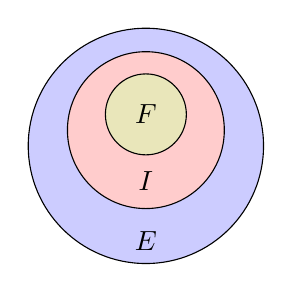
\begin{tikzpicture}[scale=1.0,transform shape]
\node[set,fill=blue!20,text width=3cm,label={[below=70pt of rea]$E$}] 
  (nat) at (0,-0.4)  (rea) {};
\node[set,fill=red!20,text width=2cm,label={[below=40pt of int]$I$}] 
  (int) at (0,-0.2)  {};
\node[set,fill=olive!20,text width=1cm] (nat) at (0,0) {$F$};
\end{tikzpicture}
\end{center}
\caption{Field extensions $E \supset I \supset F$.}
\end{figure}

Since $\alpha \in E$ has degree of $n$ over $F$, the minimal polynomial $p(x)$ of $\alpha$ over $F$ has degree of $n$.

Assume the minimal polynomial of $\alpha$ over $I$ is $p_1 (x)$, it has degree of $s$. $p(x)$ is also a polynomial over $I \supset F$ with $p(\alpha)=0$, but since $p_1(x)$ is minimal polynomial of $\alpha$ over $I$, this implies $s \leq n$. 

Assume the degree of $I(\alpha)$ over $F(\alpha)$ is $t$. Then
\begin{align*}
& (I(\alpha) : F) = (I(\alpha) : F(\alpha) ) (F(\alpha): F) = t n \\
& (I(\alpha) : F) = (I(\alpha) : I) (I: F) = sm
\end{align*}
This implies that $tn = sm$, thus $n | sm$. Note that $(n,m)=1$, so $n |s$. From $s \leq n$, this gives $s = n$. Thus, $\alpha$ has degree of $n$ over $I$. 

\end{proof}



\begin{exercise}
Suppose a field with $char(F) \neq 2$. $E$ is a field extension of $F$, with
\begin{align*}
(E:F) = 4 .
\end{align*}

Prove that there exists a $2$-degree field extension $I$ of $F$, with $F \subseteq I \subseteq E$ \underline{iff} $E=F(\alpha)$ with the minimal polynomial of $\alpha$ over $F$ is
\begin{align*}
p(x) = x^4 + ax^2 + b
\end{align*}

\end{exercise}

\begin{proof}
\begin{itemize}
\item{Assume $E=F(\alpha)$ with the minimal polynomial of $\alpha$ over $F$ is
\begin{align*}
p(x) = x^4 + ax^2 + b
\end{align*}

Consider $I = F(\alpha^2)$. Obviously, $F \subseteq I \subseteq E$.

{\color{red} $?:$ $p(x) = x^4 + ax^2 + b $ is irreducible over $F$, so $x^2 + ax + b$ is also irreducible over $F$.}

But then
\begin{align*}
(\alpha^2)^2 + a (\alpha^2) + b = \alpha^4 + a \alpha^2 + b = 0, \quad \mbox{by } p(\alpha) = 0
\end{align*}

So $x^2 + a x + b $ is the minimal polynomial of $\alpha^2$ over $F$. Thus, $I = F(\alpha^2)$ is the 
$2$-degree field extension of $F$.
}
\item{On the other direction, assume 
\begin{align*}
F \subseteq I \subseteq E, \quad (I:F)=2, \quad (E:F)=4 .
\end{align*}


\begin{enumerate}
\item{Obviously, $(I:F)=2$ and $(E:F)=4$ imply that $(E:I) = 2$. We can find $\theta \in E$ and $\theta \not \in I$. $\theta $ has degree of $2$ over $I$, with its minimal polynomial over $I$ having the form:
\begin{align*}
x^2 + \beta x + \gamma , \quad \theta ^2 + \beta \theta + \gamma = 0, \quad \beta, \, \gamma \in I
\end{align*}

Since $char(F) \neq 2$, we can write $\dfrac{\beta}{2}$.
\begin{align*}
(\theta + \frac{\beta}{2})^2 = \theta^2 + \beta \theta + \frac{\beta^2}{4} + \gamma - \gamma = \frac{\beta^2}{4} - \gamma .
\end{align*}

Denote $\omega = \theta + \dfrac{\beta}{2}$ and $\delta = \dfrac{\beta^2}{4} - \gamma$. Then $E = E(\omega)$ and $\omega$ has minimal polynomial over $I$ as 
\begin{align*}
x^2 - \delta , \quad \delta \in I
\end{align*}
}
\item{\label{exercise_4_3_3_step2}If $\delta \in I$ but $\delta \not \in F$, then by $(I:F)=2$, $\delta$ has minimal polynomial over $F$ 
\begin{align*}
x^2 + a x + b, \quad a, \, b \in F .
\end{align*}

Since $(\theta + \dfrac{\beta}{2})^2 = \dfrac{\beta^2}{4} - \gamma$, which is $\\omega^2 = \delta $, the minimal polynomial of $\delta $ over $F$ shows $\omega^4 + a \omega^2 + b = 0$.

Notice $I = F(\delta)$ ({\color{red} by $\delta$ degree of $2$ over $F$?}), so $E = I(\omega)= F(\delta, \omega) = F(\omega)$ ({ \color{red} since $\delta$ is a polynomial of $\omega$, $\delta = \omega^2$?}).

By assumption, $(E:F)=4$, so $\omega$ has minimal polynomial over $F$ with degree of $4$, which is
\begin{align*}
x^4 + a x^2 + b
\end{align*}
}
\item{If $\delta \in F \subseteq I$, then since $(I:F)= 2$, we can find $\lambda \in I$ and $\lambda \not \in F$. Take
\begin{align*}
\omega' = \omega ( 1 + \lambda)
\end{align*}
Then,
\begin{align*}
\omega'^2 = \omega^2 ( 1+ 2 \lambda + \lambda^2 )
\end{align*}
Since $\lambda \not \in F$, $( 1+ 2 \lambda + \lambda^2 ) \not \in F$, with $\omega^2 = \delta \in F$, we derive $\omega' \not \in F$. Denote $\delta ' := \omega'^2 \not \in F$. So $\delta'$ has minimal polynomial over $F$ as
\begin{align*}
x^2 + a x + b
\end{align*}
Apply the same argument as in Step \ref{exercise_4_3_3_step2}, we have $E = F(\omega')$ and $\omega'$ has minimal polynomial over $F$ as
\begin{align*}
x^4 + ax^2 + b .
\end{align*}
}
\end{enumerate}
}
\end{itemize}
\end{proof}

\begin{exercise}
$E$ is a finite field extension of $F$. There exists finite number of elements $\alpha_1$, $\alpha_2$, $\ldots$, $\alpha_m \in E$ such that 
\begin{align*}
E = F(\alpha_1, \alpha_2, \ldots, \alpha_m ) .
\end{align*}
\end{exercise}

\begin{soln}
Assume $(E:F)=m$, and consider $E$ as a vector space over $F$. Then there exists basis of $E$ as $\alpha_1$, $\alpha_2$, $\ldots$, $\alpha_m$. Obviously,
\begin{align*}
E = F(\alpha_1, \alpha_2, \ldots, \alpha_m ) .
\end{align*}
\end{soln}

\begin{exercise}
$F$ is a field of rational numbers. Add complex number for field extension:
\begin{align*}
& E_1 = F(2^{\frac{1}{3}}, 2^{\frac{1}{3} i}) \\
& E_2 = F(2^{\frac{1}{3}}, 2^{\frac{1}{3}} \omega i), \quad \omega = \frac{-1 + \sqrt{3} i}{2}, \mbox{ with } \omega^3 = 1 .
\end{align*}

Prove that
\begin{align*}
& (E_1, F(2^{\frac{1}{3}}) ) = 2, \quad (E_1, F) = 6 \\
& (E_2, F(2^{\frac{1}{3}}) ) = 4, \quad (E_2, F) = 12
\end{align*}


\end{exercise}

\begin{proof}
$F \subseteq F(2^{\frac{1}{3}}) \subseteq F(2^{\frac{1}{3}}, i) = F(2^{\frac{1}{3}}, 2^{\frac{1}{3}} i) = E_1$.

$i \not \in F(2^{\frac{1}{3}})$. $i $ is a root of $x^2 + 1$, so $(E_1: F(2^{\frac{1}{3}}) = 2$.

$2^{\frac{1}{3}} \not \in F$, $2^{\frac{1}{3}}$ is a root of the irreducible polynomial $x^3 -2$ over $F$, so $(F(2^{\frac{1}{3}}): F) = 3$.

Thus,
\begin{align*}
(E_1 :F) = \big( E_1: F(2^{\frac{1}{3}} \big) \big( F(2^{\frac{1}{3}}): F \big) = 2 \times 3 = 6 .
\end{align*}

On the other hand, $E_2 = F(2^{\frac{1}{3}}, 2^{\frac{1}{3}} \omega i)$. So $\omega i \in E_2$, and $- (\omega i )^3 = - 1 i^3 = i \in E_2$. Then again by $\omega i = \frac{-1}{2} i - \sqrt{3}{2} \in E_2$, this implies $\sqrt{3} \in E_2$. 

Therefore,
\begin{align*}
E_2 = F(2^{\frac{1}{3}}, 2^{\frac{1}{3}} \omega i) = F(2^{\frac{1}{3}}, \sqrt{3}, i) \supseteq F(2^{\frac{1}{3}}, \sqrt{3}) \supseteq F(2^{\frac{1}{3}}) \supseteq F
\end{align*}

$\big( E_2 : F(2^{\frac{1}{3}}, \sqrt{3}) \big) = \big( F(2^{\frac{1}{3}}, \sqrt{3}, i) :  F(2^{\frac{1}{3}}, \sqrt{3})  \big)  = 2$.

$\sqrt{3} \not \in F(2^{\frac{1}{3}}) $, otherwise $F(2^{\frac{1}{3}}) \supseteq F(\sqrt{3})  $ makes contradiction with $ \big( F(2^{\frac{1}{3}}) : F \big) = 3$ and $ \big( F(\sqrt{3}) : F \big) = 2$ by Theorem \ref{theorem_4_3_1_finite_extension_transitivity}.

Thus, $\big( F(2^{\frac{1}{3}}, \sqrt{3}) :  F(2^{\frac{1}{3}})  \big) = 2$.

With $\big( F(2^{\frac{1}{3}}) : F \big) = 3$, we know
\begin{align*}
& \big( E_2 : F \big) = \big( E_2 : F(2^{\frac{1}{3}}, \sqrt{3}) \big) \, \big( F(2^{\frac{1}{3}}, \sqrt{3}) :  F(2^{\frac{1}{3}})  \big) \, \big( F(2^{\frac{1}{3}}) : F \big) \\
& = 2 \times 2 \times 3 = 12
\end{align*}

\end{proof}

\section{Splitting Field (分裂域)}

\begin{theorem}
\label{theorem_4_4_1_fundamental_thm_algebra}
Every $n$ degree polynomial in $\mathbb{C}[x]$ over complex number field $\mathbb{C}$ has $n$ roots.
\end{theorem}

In other words, any polynomial in $\mathbb{C}[x]$ has roots.

\begin{definition}
\label{def_algebraic_closed_1}
Given a field $E$ and its polynomial ring $E[x]$ over $E$. If every polynomial $f(x) \in E[x]$ factors as a product of linear factor $(x + a_i)$, then $E$ has no further algebraic field extension. We call $E$ \textbf{algebraic closed}.
\end{definition}

We can have alternative definition for algebraic closure.

\begin{definition}
\label{def_algebraic_closed_2}
Given a field $F$, and its field extension $E$, we define \textbf{algebraic closure of $F$ in $E$} as a field with all elements in $E$ are algebraic over $F$.

That is, a field $F$ is \textbf{algebraically closed} if every non-constant polynomial in $F[x]$ has a root.
\end{definition}


\begin{theorem}
\label{theorem_4_4_extra_1_algebraic_close_iff}
A field $F$ is algebraically closed \underline{iff} every non-constant polynomial in $F[x]$ factors into linear factors over $F[x]$.
\end{theorem}

\begin{proof}
Assume $F$ is algebraically closed. Then, for any non-constant polynomial $p(x) \in F[x]$ has $p(\alpha) = 0$, for some $\alpha \in F$.

Assume the form of $p(x)$ with $p(\alpha)$ as
\begin{align*}
& p(x) = a_n x^n + a_{n-1} x^{n-1} + \ldots + a_1 x + a_0 \\
& p(\alpha) = a_n \alpha^n + a_{n-1} \alpha^{n-1} + \ldots + a_1 \alpha + a_0 = 0
\end{align*}

Obviously, $p(x) = p(x) - p(\alpha)$, which gives
\begin{align*}
p(x) &= a_n (x^n - \alpha^n) + a_{n-1} (x^{n-1} - \alpha^{n-1} ) + \ldots + a_1 (x - \alpha) \\
&=(x-\alpha) (\ldots )
\end{align*}

That is $(x-\alpha)$ is a linear factor of $p(x)$. We can write
\begin{align*}
p(x) = (x-\alpha)q_1(x)
\end{align*}
with $deg(q_1(x)) < deg(p(x))$.

Since $deg(p(x))$ is finite, this process will stop after finite steps with
\begin{align*}
p(x) = (x-\alpha) (x - \beta) \ldots
\end{align*}
Thus, we have $p(x)$ as a product of linear factors.

Conversely, assume for any non-constant polynomial $p(x) \in F[x]$, $p(x)$ can be factored as the product of linear factors, such as
\begin{align*}
p(x) = (x-\alpha) \ldots, \quad \alpha \in F
\end{align*}

Obviously, $p(\alpha)=0$. Thus, $\alpha \in F$ is a root of $p(x)$. So by Definition \ref{def_algebraic_closed_2} of a field being algebraically closed, $F$ is algebraically closed.


\end{proof}


\begin{corollary}
\label{corollary_4_4_1_alge_closed_field_no_proper_extension}
An algebraically closed field $F$ has no proper algebraic extension $E$.
\end{corollary}

\begin{proof}
Suppose $E$ is field extension of $F$. Then $F \subseteq E$.

Take any element $\alpha \in E$. The minimal polynomial of $\alpha$ over $F$ is $p(x) \in F[x]$. $p(x)$ factors into linear factors by Theorem \ref{theorem_4_4_extra_1_algebraic_close_iff} since $F$ is algebraically closed.

Note that minimal polynomial is irreducible, this implies that $p(x) \in F[x]$ is linear, with the form
\begin{align*}
p(x) = x- \alpha .
\end{align*}

Since $p(x) \in F[x]$, $\alpha \in F$.

This means $\forall \alpha \in E \implies \alpha \in F$. This is $E \subseteq F$.

Therefore, we show $E = F$.
\end{proof}

We have the Fundamental Theorem of Algebra in different form.

\begin{theorem}
\label{theorem_4_4_1_alternative_fundamental_thm_algebra}
The field of complex numbers is algebraically closed.
\end{theorem}


We use the concept of splitting field for a weaker version of Fundamental Theorem of Algebra.

\begin{definition}
\label{def_splitting_field}
Suppose a field $F$ with its field extension $E$. Give a $n$-degree polynomial $f(x) \in F[x]$, $E$ is \textbf{a splitting field of $f(x)$ over $F$} if:

\begin{enumerate}
\item{$f(x)$ factors into product of linear factors in $E[x]$ with
\begin{align*}
f(x) = a_n (x-\alpha_1)(x-\alpha_2) \ldots (x-\alpha_n), 
\quad \alpha_i \in E ;
\end{align*}
}
\item{In a field $I$ with $F \subseteq I \subseteq E$, $f(x)$ can not factor into product of linear factors in $I[x]$.}
\end{enumerate}

\end{definition}

\begin{memo}
$E$ is a minimal field that $f(x)$ factors into product of linear factors.

Splitting field is a weaker concept in the sense that it goes from $\forall f(x) $ in Fundamental Theorem of Algebra to $\exists f(x)$.
\end{memo}


\begin{theorem}
\label{theorem_4_4_1_orig_splitting_field_extension}
If $E$ is a splitting field of $f(x) \in F[x]$ over $F$, with
\begin{align*}
f(x) =  a_n (x-\alpha_1)(x-\alpha_2) \ldots (x-\alpha_n), 
\quad \alpha_i \in E ;
\end{align*}

then, 
\begin{align*}
E = F(\alpha_1, \alpha_2, \ldots, \alpha_n) .
\end{align*}
\end{theorem}

\begin{proof}
$E$ is field extension of $F$, $F\subseteq E$, and $\alpha_i \in E$. So,
\begin{align*}
F(\alpha_1, \alpha_2, \ldots, \alpha_n) \subseteq E
\end{align*}

On the other hand, $f(x)$ in $F(\alpha_1, \alpha_2, \ldots, \alpha_n) $ has roots $\alpha_1$, $\alpha_2$, $\ldots$, $\alpha_n$, since $f(\alpha_i) = 0$ with $\alpha_i \in F(\alpha_1, \alpha_2, \ldots, \alpha_n)$

Then,
\begin{align*}
f(x) = f(x) - f(\alpha_1) = (x- \alpha_1) q_1 (x)
\end{align*}

\begin{align*}
& f(\alpha_2) = (\alpha_2 - \alpha_1) q_1 (\alpha_2) = 0 \\
\implies & q_1 (\alpha_2) = 0, \mbox{  since }( \alpha_2 \neq \alpha_1 \iff \alpha_2 - \alpha_1 \neq 0)
\end{align*}

So,
\begin{align*}
& q_1 (x) = q_1 (x) - q_1 (\alpha_2) = (x-\alpha_2) q_2 (x) \\
\implies & f(x) = (x- \alpha_1) (x-\alpha_2) q_2 (x) 
\end{align*}
and 
\begin{align*}
& f(\alpha_3) = 0 \implies q_2 (\alpha_3) =0, \mbox{ with } \\
& q_2 (x) = q_2 (x) - q_2 (\alpha_3) = (x - \alpha_3) q_3 (x) \\
\implies & f(x) = (x- \alpha_1) (x-\alpha_2) (x-\alpha_3) q_3 (x)
\end{align*}
and so on.

Since $f(x)$ has finite degree, the process above stops after finite steps and we have
\begin{align*}
f(x) =  (x- \alpha_1) (x-\alpha_2) \ldots (x-\alpha_n) .
\end{align*}

This means $f(x)$ factors as product of linear factors in $F (\alpha_1, \alpha_2, \ldots, \alpha_n) = F[\alpha_1, \alpha_2, \ldots, \alpha_n]$.

By definition of splitting field, $E$ is the minimal field that $f(x)$ factors as product of linear factors. This implies $E \subseteq F (\alpha_1, \alpha_2, \ldots, \alpha_n) $.

Therefore, in summary, it shows $E = F (\alpha_1, \alpha_2, \ldots, \alpha_n) $.

\end{proof}

The following theorem tells the existence of a splitting field.

\begin{theorem}
\label{theorem_4_4_2_existence_splitting_field}
Given a $n$-degree polynomial $f(x) \in F[x]$ over a field $F$, there exists a splitting field $E$ of $f(x)$ over $F$.
\end{theorem}


\begin{proof}
Note that $F$ is a field, so $F[x]$ is a UFD. Thus, $f(x) \in F[x]$ has unique factorization. We can write as
\begin{align*}
f(x) = f_1 (x) g_1 (x), \quad f_1 (x), \, g_1 (x) \in F[x]
\end{align*}
where $f_1 (x) $ is an irreducible monic polynomial (with leading coefficient $=1$). By Theorem \ref{theorem_4_2_3_existence_simple_alge_extension}, $f_1(x)$ has simple algebraic extension $E_1 = F(\alpha_1)$ of $F$, where the minimal polynomial of $\alpha_1$ is $f_1(x) \in F[x]$.  

This implies that $f(\alpha_1 ) =0 $ in $E_1$, thus we have in $F[x]$ that
\begin{align*}
(x-\alpha_1) | f(x) .
\end{align*}

Thus, we can write in $E_1[x] \supseteq F[x]$ 
\begin{align*}
f(x) = (x- \alpha_1) f_2 (x) g_2 (x), \quad f_2 (x) , g_2 (x) \in E_1 [x]
\end{align*}
where $f_2(x)$ is an irreducible monic polynomial in $E_1 [x]$.

Apply again Theorem \ref{theorem_4_2_3_existence_simple_alge_extension} for $f_2 (x)$, $f_2(x)$ has simple algebraic extension $E_2 = E_1 (\alpha_2) = F(\alpha_1) (\alpha_2) = F(\alpha_1, \alpha_2)$ where the minimal polynomial of $\alpha_2$ is $f_2 (x) \in E_1 [x]$ with $f_2 (\alpha_2) = 0$.

Then, in $E_2 [x]$ we can write
\begin{align*}
f(x) = (x-\alpha_2) (x - \alpha_2) f_3 (x) g_3(x),\quad  f_3(x), g_3(x) \in E_2 [x]
\end{align*}
where $f_3(x)$ is an irreducible monic polynomial in $E_2 [x]$.

Apply again Theorem \ref{theorem_4_2_3_existence_simple_alge_extension} for $f_3(x) $, $f_3(x)$ has simple algebraic extension $E_3 = E_2 (\alpha_3) = F(\alpha_1, \alpha_2, \alpha_3)$ where the minimal polynomial of $\alpha_3$ is $f_3(x) \in E_2 [x]$ with $f_3 (\alpha_3)=0$.

This process continues after finite step, up to:
\begin{align*}
f(x) = (x- \alpha_1 ) (x - \alpha_2 ) \ldots (x - \alpha_n)
\end{align*}
in $E[x]$ with
\begin{align*}
E = F(\alpha_1, \alpha_2 , \ldots, \alpha_n).
\end{align*}


\end{proof}


Now we investigate the question: Given a polynomial $f(x)$, its splitting field is isomorphic or not?


\begin{lemma}
\label{lemma_4_4_1_poly_field_iso}
Suppose $L$ and $\overline{L}$ are fields, $ L \cong \overline{L}$. Then
\begin{align*}
L[x] \cong \overline{L} [x] .
\end{align*}
\end{lemma}

\begin{proof}
Consider the isomorphic mapping
\begin{align*}
a \in L \cong \overline{a} \in \overline{L} .
\end{align*}

From there, we construct
\begin{align*}
\phi : L[x] \mapsto \overline{L}[x], \quad \phi( \sum_{i=0} ^n a_i x^i ) = \sum_{i=0} ^n \overline{a_i} x^i
\end{align*}

We want to show $\phi$ is isomorphism between $L[x]$ and $\overline{L} [x]$:
\begin{enumerate}
\item{$\phi$ is well-defined: every element $\sum_{i=0} ^n a_i x^i \in L[x]$ maps to one element $\sum_{i=0} ^n \overline{a_i} x^i \in \overline{L}[x]$. }
\item{$\phi$ is surjective: every element $\sum_{i=0} ^n \overline{a_i} x^i \in \overline{L}[x]$ has one corresponding element $\sum_{i=0} ^n a_i x^i \in L[x]$;}
\item{$\phi$ is injective: Suppose $\overline{f} (x) = \overline{g} (x)$ for $\overline{f}(x)$, $\overline{g}(x) \in \overline{L}[x] $, this implies their coefficients $\overline{a_i} = \overline{b_i}$ where $\overline{a_i}$ are coefficients of $\overline{f}(x)$ and $\overline{b_i}$ are coefficients of $\overline{g}(x)$. By isomorphism between $L$ and $\overline{L}$, we have $a_i = b_i$, and thus $f(x) = g(x)$ for $f(x)$ is the preimage of $\overline{f}(x)$ in $L[x]$ and $g(x)$ is the preimage of $\overline{g}(x)$ in $L[x]$.
}
\item{$\phi$ is homomorphism: Suppose
\begin{align*}
& f(x) = \sum_{i=0} ^n a_i x^i  \mapsto \overline{f} (x) = \sum_{i=0} ^n \overline{a} x^i \\
& g(x) = \sum_{i=0} ^n b_i x^i  \mapsto \overline{g} (x) = \sum_{i=0} ^n \overline{b} x^i  
\end{align*}

\begin{align*}
\phi \big(f(x) + g(x) \big) &= \phi\big( \sum_{i=0} ^n (a_i + b_i) x^i   \big) \\
&= \sum_{i=0} ^n \big( \overline{a_i + b_i} \big) x^i \\
&=  \sum_{i=0} ^n \big( \overline{a}_i + \overline{b}_i \big) x^i , \quad  \mbox{ by additio on $\overline{L}$} \\
&= \sum_{i=0} ^n \overline{a} x^i + \sum_{i=0} ^n \overline{b} x^i  \\
&= \overline{f} (x) + \overline{g} (x)
\end{align*} 

\begin{align*}
\phi\big( f(x) g(x) \big) &= \phi \big( \sum_k \big( \sum_{i+j = k} a_i b_j \big) x^k \big) \\
&= \sum_k \big( \sum_{i+j = k} \overline{a_i b_j } \big) x^k \\
&= \sum_k \big( \sum_{i+j = k} \overline{a}_i \overline{b}_j  \big) x^k \\
& = \overline{f}(x) \overline{g}(x)
\end{align*}
}
\item{Summing up, $\phi$ is isomorphic between $L[x]$ and $\overline{L}[x]$.}
\end{enumerate}

Therefore, we just show $L[x] \cong \overline{L}[x]$.

\end{proof}

\begin{lemma}
\label{lemma_4_4_2_simple_extension_field_iso}
Suppose $L$ and $\overline{L}$ are fields, $ L \cong \overline{L}$. $p(x) \in L[x]$ is irreducible monic polynomial. $p(x)$ has corresponding irreducible polynomial $\overline{p}(x) \in \overline{L}[x] $.

Assume $L(\alpha)$ is simple algebraic field extension of $\alpha$ of $L$, where the minimal polynomial of $\alpha$ over $L$ is $p(x) \in L[x] $ with $p(\alpha)=0$.

Assume $\overline{L}( \overline{\alpha} )$ is simple algebraic field extension of $\overline{\alpha}$ of $\overline{L}$, where the minimal polynomial of $\overline{\alpha}$ over $\overline{L}$ is $\overline{p}(x) \in \overline{L} [x] $ with $\overline{p} ( \overline{\alpha})=0$.

Then, there exists isomorphism between $L(\alpha)$ and $\overline{L} (\overline{\alpha})$. This isomorphism keeps the isomorphism between $L \subset L(\alpha)$ and $\overline{L} \subset \overline{L}(\overline{\alpha})$.

\end{lemma}

\begin{proof}
Suppose the isomorphism between $L$ and $\overline{L}$ with
\begin{align*}
\forall a \in L \iff \overline{a} \in \overline{L} .
\end{align*}

Assume the degree of $p(x)$ is $n$, thus $deg(\overline{p} (x) ) = n$..

Construct a mapping
\begin{align*}
\phi : L(\alpha) \longrightarrow \overline{L} (\overline{\alpha}), \quad \sum_{i=0} ^{n-1} a_i \alpha^i \in L(\alpha) \mapsto \sum_{i=0} ^{n-1} \overline{a}_i \overline{\alpha}^i \in \overline{L} (\overline{\alpha}).
\end{align*}

We want to show $\phi$ is isomorphism. Analogous to the reasoning in the proof of Lemma \ref{lemma_4_4_1_poly_field_iso}, we have
\begin{enumerate}
\item{$\phi$ is well-defined, and $\phi: a \mapsto \overline{a}$;}
\item{$\phi$ is surjective;}
\item{$\phi$ is injective.}
\end{enumerate}

We are left to show $\phi$ is homomorphism: Suppose
\begin{align*}
& f(\alpha) = \sum_{i=0} ^{n-1} a_i \alpha^i  \mapsto \overline{f} ( \overline{\alpha} ) = \sum_{i=0} ^{n-1} \overline{a}_i \, \overline{\alpha}^i \\
& g(\alpha) = \sum_{i=0} ^{n-1} b_i \alpha^i  \mapsto \overline{g} (\overline{\alpha}) = \sum_{i=0} ^{n-1} \overline{b}_i \, \overline{\alpha}^i  
\end{align*}

\begin{align*}
\phi \big(f( \alpha ) + g( \alpha) \big) &= \phi\big( \sum_{i=0} ^{n-1} (a_i + b_i) \alpha^i   \big) \\
&= \sum_{i=0} ^{n-1}\big( \overline{a_i + b_i} \big) \overline{\alpha}^i \\
&=  \sum_{i=0} ^{n-1} \big( \overline{a}_i + \overline{b}_i \big) \overline{\alpha}^i \\
&= \sum_{i=0} ^{n-1} \overline{a}_i \overline{\alpha}^i + \sum_{i=0} ^{n-1} \overline{b}_i \overline{\alpha}^i  \\
&= \overline{f} (\overline{\alpha} ) + \overline{g} ( \overline{\alpha})
\end{align*} 

On the other hand, $f(x) g(x)  \in L[x]$. This implies 
\begin{align*}
f(\alpha) g(\alpha) = r(\alpha) .
\end{align*}
where
\begin{align*}
f(x) g(x) = p(x) q(x) + r(x), \quad deg(r(x)) = 0, \mbox{ or } deg(r(x)) < deg(p(x)) .
\end{align*}

By Lemma \ref{lemma_4_4_1_poly_field_iso}, 
\begin{align*}
& f(x) g(x) = p(x) q(x) + r(x) \\
& \implies \overline{f} (x) \overline{g} (x) = \overline{p} (x) \overline{q} (x) + \overline{r} (x) \\
& \implies \overline{f}(\overline{\alpha}) \overline{g} (\overline{\alpha}) = \overline{p} ( \overline{\alpha} ) \overline{q} (\overline{\alpha}) + \overline{r} ( \overline{\alpha} ) =\overline{r} ( \overline{\alpha} )  , \quad \mbox{ since } \overline{p} (\overline{\alpha} ) = 0
\end{align*}

This means
\begin{align*}
f(\alpha) g(\alpha) = r(\alpha) \implies \overline{f}(\overline{\alpha}) \overline{g} (\overline{\alpha}) = \overline{r} ( \overline{\alpha} )
\end{align*}

Thus, we just show $\phi$ is a homomorphism, and therefore $\phi$ is isomorphic between $L(\alpha) $ and $\overline{L} (\overline{\alpha})$. Moreover, $\phi$ reserves the isomorphism between $L$ and $\overline{L}$.

\end{proof}

Now we prove the uniqueness of the splitting field.

\begin{theorem}
\label{theorem_4_4_3_uniqueness_splitting_field}
Suppose fields $F$ and $\overline{F}$, with $F \cong \overline{F}$. The $n$-degree polynomial $f(x) \in F[x]$ has the corresponding polynomial $\overline{f}(x) \in \overline{F}[x]$ in the sense of Lemma \ref{lemma_4_4_1_poly_field_iso}.

Further assume
\begin{itemize}
\item{$E= F(\alpha_1, \alpha_2, \ldots, \alpha_n)$ is a splitting field of $f(x)$ over $F$;}
\item{$\overline{E}= \overline{F} ( \beta_1, \beta_2, \ldots, \beta_n)$ is a splitting field of $\overline{f} (x)$ over $ \overline{F}$.}
\end{itemize}

Then, there exists a isomorphism
\begin{align*}
\phi : E \iff \overline{E}
\end{align*}
where
\begin{itemize}
\item{$\phi$ keeps isomorphism $F \cong \overline{F}$; }
\item{After proper rearrangement, 
\begin{align*}
\alpha_i \iff \beta_i .
\end{align*}
}
\end{itemize}

\end{theorem}

\begin{proof}
Prove by mathematical induction:

Note that by $F \cong \overline{F}$, there exists $a \in F \iff \overline{a} \in \overline{F}$.

\begin{enumerate}
\item{If $k=0$, then $E = F$ and $\overline{E} = \overline{F}$. So $F \cong \overline{F} \implies E \cong \overline{E}$.}
\item{Suppose if $k < n$, there exists
\begin{align*}
L := F(\alpha_1, \alpha_2, \ldots, \alpha_k) \cong \overline{L} := \overline{F}(\beta_1, \beta_2, \ldots, \beta_k) , \quad \alpha_i \iff \beta_i 
\end{align*}
by proper rearrangement of $\beta_1$, $\beta_2$, $\ldots$, $\beta_k$.

Then, $L$ and $\overline{L}$ are fields. So we can consider $L[x]$ and $\overline{L}[x]$. Suppose $f(x) \in L[x]$, we can factor $f(x)$ as
\begin{align*}
f(x) = (x- \alpha_1) (x - \alpha_2) \ldots (x - \alpha_k) p_k (x) q_k (x)
\end{align*}
where $p_k (x)$ is irreducible monic polynomial of $L[x]$.

By Lemma \ref{lemma_4_4_1_poly_field_iso}, there exists the corresponding polynomial $\overline{f} (x) \in \overline{L}[x]$ such that
\begin{align*}
\overline{f}(x) = (x - \beta_1) (x - \beta_2) \ldots (x - \beta_k) \overline{p_k} (x) \overline{q_k} (x)
\end{align*}
where $\overline{p_k} (x)$ is irreducible monic polynomial of $\overline{L}[x]$.

Consider in the field extensions $F(\alpha_1, \alpha_2, \ldots , \alpha_n)$ and $\overline{F}(\beta_1, \beta_2, \ldots , \beta_n$, we can factor
\begin{align*}
p_k(x) q_k(x) = (x- \alpha_{k+1}) \ldots (x - \alpha_{n} ) \\
\overline{p_k} (x) \overline{q_k} (x) = (x - \beta_{k+1} ) \ldots (x - \beta_{n}) .
\end{align*}

After rearragement of $\alpha_{k+1}$, $\ldots$, $\alpha_{n}$ and $\beta_{k+1}$, $\ldots$, $\beta_{n}$, we can have
\begin{align*}
p_k (\alpha_{k+1} ) = 0, \quad \overline{p_k} (\beta_{k+1} ) = 0.
\end{align*}

Apply Lemma \ref{lemma_4_4_2_simple_extension_field_iso}, there exists isomorphism between $L(\alpha_{k+1}$ and $\overline{L}(\beta_{k+1}$, which is
\begin{align*}
L(\alpha_{k+1}) = F(\alpha_1, \alpha_2, \ldots, \alpha_{k+1}) \cong \overline{L} (\beta_{k+1}) = \overline{F}(\beta_1, \beta_2, \ldots, \beta_{k+1}),
\end{align*}
with $\alpha_i \iff \beta_i$, $i = 1, \ldots, k+1$.
}
\end{enumerate}

\end{proof}


\begin{memo}
By Corollary \ref{corollary_3_6_1_n_degree_n_roots}, $n$-degree polynomial over some field has at most $n$ roots.

Theorem \ref{theorem_4_4_2_existence_splitting_field} tells there exists some field extension where $f(x)$ has $n$ roots.

Theorem \ref{theorem_4_4_3_uniqueness_splitting_field} tells $f(x)$ via different field extension has the same $n$ roots in the sense of isomorphism.

So, this means that given any polynomial $f(x)$ over any field $F$, the roots of $f(x)$ is 'fixed'.

In some sense, if given the polynomial $f(x)$, we can use splitting field extension to replace the Fundamental Theorem of Algebra.

\end{memo}


Here below shows an important property of splitting field.

\begin{theorem}
\label{theorem_4_4_4_linear_factoring_splitting_field}
Suppose $E$ is a splitting field of some polynomial $f(x) \in F[x]$ over $F$. 

Given any element $\beta \in E$, then the minimal polynomial of $\beta$ over $F$ factors into a product of linear factors in $E$. 
\end{theorem}

\begin{proof}
Let the splitting field of $f(x)$ over $F$ is
\begin{align*}
E = F(\alpha_1 , \alpha_2, \ldots, \alpha_n).
\end{align*}
where $f(\alpha_i) = 0$. (Obviously, $\alpha_i$ is algebraic over $F$.)

Prove by contradiction: Assume $\beta$ has the minimal polynomial $g(x)$ over $F$, with $g(\beta)=0$. Further assume $g(x)$ can not be factored as product of linear factors. Thus, we can write
\begin{align*}
g(x) = (x- \beta) p(x) g_1 (x), \quad p(x), g_1 (x) \in F[x] \subseteq E[x].
\end{align*}
where $p(x)$ is irreducible monic polynomial.

By our assumption, $deg(p(x)) = m > 1$.

Let $p(x)$ be the minimal polynomial of $\beta'$ over $E$, with $p(\beta') = 0$. 

Note that
\begin{align*}
g(\beta') = (\beta' - \beta) p(\beta') g_1 (\beta') = 0, \quad \mbox{by } p(\beta') = 0 .
\end{align*}

By Theorem \ref{theorem_4_2_iso_simple_alge_extension}, $F(\beta)$ and $F(\beta')$ are simple algebraic extension of $F$. $\beta$ and $\beta'$ has the same minimal polynomial over $F$, $p(x)$, then we have
\begin{align*}
F(\beta) \cong F(\beta') .
\end{align*}

By Lemma \ref{lemma_4_4_1_poly_field_iso}, $F(\beta) \cong F(\beta')$ implies $F(\beta)[x] \cong F(\beta')[x]$. 

Also, this isomorphism keeps $f(x) \longleftrightarrow f(x)$.

By Theorem \ref{theorem_4_4_3_uniqueness_splitting_field}, the splitting field of $f(x)$ over $F(\beta)$ is isomorphic to the splitting field of $f(x)$ over $F(\beta')$.

Note that $F(\beta, \alpha_1, \alpha_2, \ldots, \alpha_n)$ is the splitting field of $f(x)$ over $F(\beta)$, while $F(\beta', \alpha_1, \alpha_2, \ldots, \alpha_n)$ is the splitting field of $f(x)$ over $F(\beta')$. Thus,
\begin{align*}
& F(\beta, \alpha_1, \alpha_2, \ldots, \alpha_n) \cong F(\beta', \alpha_1, \alpha_2, \ldots, \alpha_n) \\
\implies & \big( F(\beta, \alpha_1, \alpha_2, \ldots, \alpha_n) : F\big)  = \big( F(\beta', \alpha_1, \alpha_2, \ldots, \alpha_n) : F \big) .
\end{align*} 

Obviously, we have
\begin{align*}
\big( F(\beta', \alpha_1, \alpha_2, \ldots, \alpha_n) : F \big)  = \big( E(\beta') : E \big) \big( E: F \big) = m \big( E:F \big)
\end{align*}

Since $\beta \in E $, we have
\begin{align*}
\big( F(\beta, \alpha_1, \alpha_2, \ldots, \alpha_n) : F\big) = \big( F(\beta, \alpha_1, \alpha_2, \ldots, \alpha_n) : E \big) \big( E : F \big) =  \big( E : F \big)
\end{align*}

Because $deg(p(x)) = m > 1$ from our assumption, we obtain contradiction. 

\end{proof}


\begin{exercise}
Prove that in the field of rational numbers, the splitting field of the polynomial $x^4 + 1 $ is a simple field extension $F(\alpha)$, where $a$ is one of the roots of $x^4 + 1$. 
\end{exercise}

\begin{proof}
Consider the field of complex numbers $\mathbb{C}$ where polynomial has roots. The polynomial $x^4 + 1$ in $\mathbb{C}$ has $4$ roots:
\begin{align*}
\alpha_1 = \frac{sqrt{2}}{2} ( 1 + i), \quad \alpha_2 = \frac{sqrt{2}}{2} ( 1 - i), \\
\alpha_3 = - \alpha_1, \quad \alpha_4 = - \alpha_2 .
\end{align*}

Note that $\alpha_2 = - \alpha_1 ^3$, which implies 
\begin{align*}
F(\alpha_1, \alpha_2, \alpha_3, \alpha_4) = F(\alpha_1).
\end{align*}

This simple field extension $F(\alpha_1)$ is the splitting field of the polynomial $x^4 + 1$ over $F$.
\end{proof}


\begin{exercise}
Suppose $F$ is a field of rational numbers. the irreducible polynomial $x^3 - a$ over $F$, with $\alpha$ is one of the roots of $x^3 - a$. Prove that $F(\alpha)$ is \underline{not} the splitting field of the polynomial $x^3 - a$ over $F$.
\end{exercise}

\begin{proof}
$x^3 - a$ has $3$ roots:
\begin{align*}
a^{\frac{1}{3}}, \quad a^{\frac{1}{3}}\omega, \quad a^{\frac{1}{3}} \omega^2, 
\end{align*}
where
\begin{align*}
\omega = \frac{-1 + \sqrt{3} i }{2}, \quad \omega^3 = 1.
\end{align*}

The splitting field of $x^3 - a$ over $F$ is
\begin{align*}
E := F\big(  a^{\frac{1}{3}}, \, a^{\frac{1}{3}}\omega, \, a^{\frac{1}{3}} \omega^2 \big) = F \big( a^{\frac{1}{3}} , \,   \omega \big)
\end{align*}

Thus, we have
\begin{align*}
 F \big( a^{\frac{1}{3}} , \,   \omega \big) \supseteq  F \big( a^{\frac{1}{3}} \big) \supseteq F .
\end{align*}

Note that $\omega \not \in  F \big( a^{\frac{1}{3}} \big) $, and $\omega $ is the root of the polynomial $x^2 + x + 1$ over $F \big( a^{\frac{1}{3}} \big) $, thus,
\begin{align*}
\big( F \big( a^{\frac{1}{3}}, \omega \big) : F \big( a^{\frac{1}{3}} \big)  \big) = 2 .
\end{align*} 

Note that $a^{\frac{1}{3}}$ is the root of irreducible polynomial $x^3 - a$ over $F$. Thus,
\begin{align*}
\big( F \big( a^{\frac{1}{3}} \big) : F \big) = 3 .
\end{align*}

Therefore,
\begin{align*}
& \big( E : F \big) \\
=& \big( F \big( a^{\frac{1}{3}} , \,   \omega \big) : F\big) \\
=& \big( F \big( a^{\frac{1}{3}} , \,   \omega \big) : F \big( a^{\frac{1}{3}} \big)  \big) \big( F\big(  a^{\frac{1}{3}} \big)  : F\big) = 2 \times 3 = 6 .
\end{align*}

$\alpha$ is a root of $x^3 - a$. Then,
\begin{align*}
\big(F(\alpha) : F  \big) = 3 .
\end{align*}
Therefore, $E \neq F(\alpha)$, which is $F(\alpha)$ is not the splitting field of the polynomial $x^3 - a$ over $F$.

\end{proof}


\begin{exercise}
Suppose the following $m$ irreducible monic polynomials over $F$:
\begin{align*}
p_1(x), \, p_2 (x), \, \ldots , \, p_m(x) .
\end{align*}

Prove that there exists a finite field extension 
\begin{align*}
F(\alpha_1, \alpha_2, \ldots, \alpha_m)
\end{align*}
where the minimal polynomial of $\alpha_i$ over $F$ is $p_i (x)$.
\end{exercise}

\begin{proof}
Consider
\begin{align*}
F(x) = p_1 (x) p_2 (x) \ldots p_m (x) .
\end{align*}

Construct $E$ as the splitting field of $f(x)$ over $F$.

$E$ has all the roots of $f(x)$, which means $\alpha_1, \alpha_2, \ldots, \alpha_m \in E$ where $\alpha_i$ is the root of $p_i (x)$. Thus,
\begin{align*}
F(\alpha_1, \alpha_2, \ldots, \alpha_m) \subseteq E .
\end{align*}

Since $p_i (x)$ is irreducible monic polynomial over $F$, they are the minimal polynomial of $\alpha_i$ over $F$. That is $\alpha_i$ is algebraic over $F$, thus $ F(\alpha_1, \alpha_2, \ldots, \alpha_m)  $ is a finite field extension of $F$.

\end{proof}


\begin{exercise}
Suppose $P$ is a field with $char(P) = p$ where $p$ is prime number. $F = P (\alpha)$ is a simple field extension of $P$. Suppose $\alpha$ is a root of the polynomial $x^p - a \in P[x]$. Is $P(\alpha)$ a splitting field of $x^p -a$ over $P$?

\end{exercise}

\begin{soln}
Since $\alpha$ is a root of $x^p -a$, thus $\alpha^p = a$. The field $P$ and thus the field $F \supset P$ has characteristic of the prime number $p$. So in $F[x]$,
\begin{align*}
x^p -a = x^p - \alpha^p  = (x - \alpha)^p .
\end{align*}

Thus, $P(\alpha)$ can be considered as the field extension by adding $p$ roots of $x^p -a$. Thus, $P(\alpha)$ is the splitting field of the polynomial $x^p -a $ over $P$.


\end{soln}





\end{document}
